% NOTE: remember to makeglossary after compile to make lists of symbol appear

\documentclass[12pt,space=onehalf,version=final,mainlanguage=english]{yathesis}
\usepackage[T1]{fontenc}
\usepackage[utf8]{inputenc}
\usepackage{lipsum} % À proscrire dans un vrai mémoire de thèse !
\usepackage{kpfonts}
\usepackage{booktabs}
\usepackage{siunitx}
\usepackage{pgfplots}
\usepackage{floatrow}	
\usepackage{caption}
\usepackage{listings}
\usepackage{microtype}
\usepackage{varioref}
\usepackage[xindy,quiet]{imakeidx}
\usepackage[autostyle]{csquotes}
\usepackage{hyperref}
\usepackage[acronyms,symbols,nonumberlist,sort=standard]{glossaries}

\usepackage{geometry}
\usepackage{tikz}
%\usepackage{graphicx}
\usepackage{subfigure}

\usepackage{algorithmicx}
\usepackage[ruled]{algorithm}
\usepackage{algpseudocode}

\usepackage{amsmath}
\usepackage{txfonts}
\usepackage{amsfonts}
\usepackage[mathscr]{euscript}
\usepackage{amsfonts}
\usepackage{dsfont}

\usepackage{colortbl}
  \newcommand{\myrowcolour}{\rowcolor[gray]{0.925}}
\usepackage{booktabs}
\usepackage{siunitx}
\usepackage{tabularx}
\usepackage{tabulary}
\usepackage{multirow}
\usepackage{morewrites}%Always room for a new write stream, permet de creer de nouveau glossaire avec la commande newglossary sinon ca ne marche pas

\usepackage[backend=bibtex,safeinputenc,style=authoryear-comp, maxnames=2, natbib=true, dashed=false]{biblatex}

% DEFINE MATH OPERATORS


% Génération de l'index :
\makeindex

% (Facultatif) Spécification de la ou des ressources terminologiques :

%\loadglsentries{auxiliaires/acronymes}
%\loadglsentries{auxiliaires/symboles}

\addbibresource{auxiliaires/bibliographie.bib}

% % % % GLOSSARIES
\renewcommand*{\glspostdescription}{}
\newglossary[slg1]{gloss-abbre}{sls1}{slo1}{Abbreviations}
\newglossary[slg2]{gloss-latin}{sls2}{slo2}{Latin symbols}
\newglossary[slg3]{gloss-math}{sls3}{slo3}{Math symbols}

\makeglossaries
\newcommand{\mynewglssymbol}[6][]{%
  \ifthenelse{\isempty{#1}}{%
    \newglossaryentry{#2}{%
      type={#6},%
      symbol={#5},%
      name={#3},%
      description={#4},%
      sort={#2}%
    }%
  }{%
    \newglossaryentry{#2}{%
      type={#6},%
      symbol={#5},%
      name={#3},%
      description={#4},%
      sort={#1}%
    }%
  }%
}

\everymath{\displaystyle}
\DeclareMathOperator*{\argmax}{\arg\!\max}
\DeclareMathOperator*{\argmin}{\arg\!\min}

\DeclareMathOperator{\sign}{sign}
\DeclareMathOperator{\prox}{prox}

\newcommand{\mybold}[1]{\ensuremath{\operatorname{\boldsymbol{#1}}}}
\newcommand{\mydef}{\triangleq}
\newcommand{\mytrans}{\intercal}
\newcommand{\mypseudo}{\dagger}
\newcommand{\myhat}[1]{\ensuremath{\operatorname{\hat{#1}}}}
\newcommand{\myexp}[1]{\ensuremath{\operatorname{\exp{ \left(#1\right)}}}}
\newcommand{\mysign}[1]{\ensuremath{\operatorname{\sign{\left(#1\right)}}}}
\newcommand{\mydot}{\cdot} 

\newcommand{\R}{{\rm I\!R}}
\newcommand{\subjectto}{\:\:\:\:\:\: s.t. \:\:\:\:\:\:}
\newcommand{\Df}{D_f}
\newcommand{\dimsh}{P}
\newcommand{\dimsl}{Q}
\newcommand{\dimth}{N}
\newcommand{\dimtl}{M}
\newcommand{\dimpsh}{p}
\newcommand{\dimpsl}{q}
\newcommand{\dimpth}{n}
\newcommand{\dimptl}{m}
\newcommand{\dimdict}{K}
\newcommand{\dimtrunc}{L}

\newcommand{\dimpacc}{r} % accumulative patch size
\newcommand{\dimpsr}{s} % searching region size
\newcommand{\nlmfilparam}{\sigma} % accumulative patch size \tau

\newcommand{\neighbor}{\mathcal{N}}
\newcommand{\mymapto}{\longmapsto}
\newcommand{\mymapfrom}{\mathrel{\reflectbox{\ensuremath{\mymapto}}}}

\newcommand{\z}{\mybold{z}}
\newcommand{\y}{\mybold{y}}
\newcommand{\x}{\mybold{x}}
\newcommand{\Z}{\mathbf{Z}}
\newcommand{\Y}{\mathbf{Y}}
\newcommand{\X}{\mathbf{X}}
\newcommand{\B}{\mathbf{B}}
\newcommand{\I}{\mathbf{I}}
\newcommand{\Diag}{\mathbf{D}}
\newcommand{\Umat}{\mathbf{U}}
\newcommand{\Vmat}{\mathbf{V}}

\newcommand{\LR}{\y}
\newcommand{\HR}{\z}
\newcommand{\LF}{\z_{lf}}
\newcommand{\HF}{\z_{hf}}
\newcommand{\HFest}{\hat{\z }_{hf}}

\newcommand{\h}{\mybold{h}}
\newcommand{\n}{\mybold{n}}
\newcommand{\boundHF}{\mybold{b}}

\newcommand{\knot}{{\circ}}
\newcommand{\ext}{{e}} % denote the generalization data for prediction

\newcommand{\Interp}{\varmathbb{I}}
\newcommand{\Sub}{\varmathbb{S}}
\newcommand{\LPF}{\varmathbb{L}}

\newcommand{\distr}{\mathscr{N}} 
\newcommand{\loss}{\mathcal{L}}

\newcommand{\normtwo}[1]{\ensuremath{\operatorname{\Arrowvert  \mathit{#1} \Arrowvert^2_2 }}}
\newcommand{\Mdist}[2]{\ensuremath{\operatorname{\Arrowvert \mathit{#1} \Arrowvert^2_{\mathit{#2}} }}}
\newcommand{\normone}[1]{\ensuremath{\operatorname{\Arrowvert \mathit{#1} \Arrowvert_1 }}}
\newcommand{\normzero}[1]{\ensuremath{\operatorname{\Arrowvert  \mathit{#1} \Arrowvert_0 }}}
\newcommand{\normp}[1]{\ensuremath{\operatorname{\Arrowvert  \mathit{#1} \Arrowvert_p }}}

\newcommand{\detmat}[1]{\ensuremath{\operatorname{\left|  \mathit{#1} \right| }}}
\newcommand{\cov}[1]{\ensuremath{\operatorname{cov \left\lbrace  \mathit{#1} \right\rbrace }}}
\newcommand{\E}[1]{\ensuremath{\operatorname{E \left[  \mathit{#1} \right] }}}
\newcommand{\tr}[1]{\ensuremath{\operatorname{tr \left\lbrace  \mathit{#1} \right\rbrace }}}
\newcommand{\Conv}{\mathop{\scalebox{1.5}{\raisebox{-0.2ex}{$\ast$}}}}

\newcommand{\pinv}[1]{\ensuremath{\operatorname{  \mathit{#1} ^\dagger}}}
%\newcommand{\featmap}[1]{\ensuremath{\operatorname{  \mathcal{F} \left(#1\right)}}}
\newcommand{\featmap}[1]{\ensuremath{\operatorname{ \varphi \left(\mathit{#1}\right)}}}

%\newcommand{\dict}{\mathds{D}}
%\newcommand{\dictco}{\mathds{A}}
\newcommand{\dict}{\mathbf{D}}
\newcommand{\dictco}{\mathbf{A}}
\newcommand{\adict}{\boldsymbol{d}}
\newcommand{\adictco}{\boldsymbol{a}}

\newcommand{\patchlow}[1]{\ensuremath{\operatorname{\mathit{\mybold{p}_{\ell}^{#1}}}}}
\newcommand{\patchhigh}[1]{\ensuremath{\operatorname{\mathit{\mybold{p}_h^{#1}}}}}
\newcommand{\dictlow}{\dict_\ell}
\newcommand{\dicthigh}{\dict_h}
\newcommand{\adictcolow}[1]{\ensuremath{\operatorname{\boldsymbol{a}_\ell^{\mathit{#1}}}}}
\newcommand{\adictcohigh}[1]{\ensuremath{\operatorname{\mathit{\boldsymbol{a}_h^{#1}}}}}
\newcommand{\adictlow}[1]{\ensuremath{\operatorname{\boldsymbol{d}_\ell^{\mathit{#1}}}}}
\newcommand{\adicthigh}[1]{\ensuremath{\operatorname{\mathit{\boldsymbol{d}_h^{#1}}}}}

\newcommand{\extractlow}[1]{\ensuremath{\operatorname{\mathcal{R}_{\ell}^{\mathit{#1}}}}}
\newcommand{\extracthigh}[1]{\ensuremath{\operatorname{\mathit{\mathcal{R}_h^{#1}}}}}
\newcommand{\extract}[1]{\ensuremath{\operatorname{\mathcal{R}^{\mathit{#1}}}}}


\newcommand{\mytrace}[1]{\ensuremath{\operatorname{\text{Tr} \left( #1 \right)}}}

% Shift+Alt+F1 before to compile glossary

% % % % % % % % % % % % % % % % ABBREVIATIONS % % % % % % % % % % % % % % % % % %
\mynewglssymbol{dns}{DNS}{\textbf{D}irect \textbf{N}umerical \textbf{S}imulation}{}{gloss-abbre}
\mynewglssymbol{piv}{PIV}{\textbf{P}article \textbf{I}mage \textbf{V}elocimetry}{}{gloss-abbre}
\mynewglssymbol{spiv}{SPIV}{\textbf{S}tereo \textbf{P}article \textbf{I}mage \textbf{V}elocimetry}{}{gloss-abbre}
\mynewglssymbol{stb}{STB}{\textbf{S}hake-\textbf{T}he-\textbf{B}ox PIV calibration}{}{gloss-abbre}
\mynewglssymbol{hwa}{HWA}{\textbf{H}ot \textbf{W}ire \textbf{A}nemometer}{}{gloss-abbre}
\mynewglssymbol{hr}{HR}{\textbf{H}igh \textbf{R}esolution}{}{gloss-abbre}
\mynewglssymbol{lr}{LR}{\textbf{L}ow \textbf{R}esolution  }{}{gloss-abbre}
\mynewglssymbol{hf}{HF}{\textbf{H}igh \textbf{F}requency}{}{gloss-abbre}
\mynewglssymbol{lf}{LF}{\textbf{L}ow \textbf{F}requency  }{}{gloss-abbre}
\mynewglssymbol{hths}{HTHS}{\textbf{H}igh-\textbf{T}ime-\textbf{H}igh-\textbf{S}pace resolution}{}{gloss-abbre}
\mynewglssymbol{lths}{LTHS}{\textbf{L}ow-\textbf{T}ime-\textbf{H}igh-\textbf{S}pace resolution}{}{gloss-abbre}
\mynewglssymbol{htls}{HTLS}{\textbf{H}igh-\textbf{T}ime-\textbf{L}ow-\textbf{S}pace resolution}{}{gloss-abbre}
\mynewglssymbol{nlm}{NLM}{\textbf{N}on- \textbf{L}ocal \textbf{M}eans}{}{gloss-abbre}
\mynewglssymbol{dl}{DL}{\textbf{D}ictionary \textbf{L}earning}{}{gloss-abbre}
\mynewglssymbol{sr}{SR}{\textbf{S}uper- \textbf{R}esolution}{}{gloss-abbre}
\mynewglssymbol{nrmse_symbol}{NRMSE}{\textbf{N}ormalized \textbf{R}oot \textbf{M}ean \textbf{S}quare \textbf{E}rror}{}{gloss-abbre}
\mynewglssymbol{rmse}{RMSE}{\textbf{R}oot \textbf{M}ean \textbf{S}quare \textbf{E}rror}{}{gloss-abbre}
\mynewglssymbol{mse}{MSE}{\textbf{M}ean \textbf{S}quare \textbf{E}rror}{}{gloss-abbre}
\mynewglssymbol{lse}{LSE}{\textbf{L}inear \textbf{S}tochastic \textbf{E}stimation or  \textbf{L}east \textbf{S}quare \textbf{E}stimation  }{}{gloss-abbre}
\mynewglssymbol{rr}{RR}{\textbf{R}idge \textbf{R}egression }{}{gloss-abbre}
\mynewglssymbol{krr}{KRR}{\textbf{K}ernel \textbf{R}idge \textbf{R}egression \textbf{}  }{}{gloss-abbre}
\mynewglssymbol{lasso}{LASSO}{\textbf{L}east \textbf{A}bsolute \textbf{S}hrinkage and \textbf{S}election \textbf{O}perator }{}{gloss-abbre}
\mynewglssymbol{re}{Re}{\textbf{Re}ynolds number}{}{gloss-abbre}
\mynewglssymbol{ns}{N-S}{\textbf{Navier}-\textbf{S}tokes}{}{gloss-abbre}
\mynewglssymbol{svd}{SVD}{\textbf{S}ingular \textbf{V}alue \textbf{D}ecomposition}{}{gloss-abbre}
\mynewglssymbol{pod}{POD}{\textbf{P}roper \textbf{O}rthogonal \textbf{D}ecomposition}{}{gloss-abbre}
\mynewglssymbol{cv}{CV}{\textbf{C}ross \textbf{V}alidation}{}{gloss-abbre}
\mynewglssymbol{loocv}{LOOCV}{\textbf{L}eave \textbf{O}ne \textbf{O}ut \textbf{C}ross \textbf{V}alidation}{}{gloss-abbre}
\mynewglssymbol{mle}{MLE}{\textbf{M}aximum \textbf{L}ikelihood \textbf{E}stimator}{}{gloss-abbre}
\mynewglssymbol{map}{MAP}{\textbf{M}aximum \textbf{A} \textbf{P}osteriori}{}{gloss-abbre}

\mynewglssymbol{pca}{PCA}{\textbf{P}rincipal \textbf{C}omponent \textbf{A}nalysis}{}{gloss-abbre}
\mynewglssymbol{odl}{ODL}{\textbf{O}nline \textbf{D}ictionary \textbf{L}earning}{}{gloss-abbre}
\mynewglssymbol{dct}{DCT}{\textbf{D}iscrete \textbf{C}osine \textbf{T}rainsform}{}{gloss-abbre}
\mynewglssymbol{lars}{LARS}{\textbf{L}east \textbf{A}ngle \textbf{R}egre\textbf{S}sion}{}{gloss-abbre}
\mynewglssymbol{sr1}{SR1}{\textbf{Super}-\textbf{R}esolution: coupling low and high resolution patches}{}{gloss-abbre}
\mynewglssymbol{sr2}{SR2}{\textbf{Super}-\textbf{R}esolution: coupling interpolated low and high resolution patches}{}{gloss-abbre}
\mynewglssymbol{sr3}{SR3}{\textbf{Super}-\textbf{R}esolution: coupling derivatives with residuals patches}{}{gloss-abbre}






% % % % % % % % % % % % % % % % LATIN SYMBOLS % % % % % % % % % % % % % % % % % % 
\mynewglssymbol{A_coor_z}{$ z $}{(coordinate in) spanwise direction}{}{gloss-latin}
\mynewglssymbol{A_coor_y}{$ y $}{(coordinate in) vertical direction}{}{gloss-latin}
\mynewglssymbol{A_coor_x}{$ x $}{(coordinate in) streamwise direction}{}{gloss-latin}
\mynewglssymbol{A_coor_t}{$ t $}{(coordinate in) time}{}{gloss-latin}
\mynewglssymbol{A_coor_loc_z}{$ \beta $}{(local coordinate in) spanwise direction}{}{gloss-latin}
\mynewglssymbol{A_coor_loc_y}{$ \alpha $}{(local coordinate in) vertical direction}{}{gloss-latin}
\mynewglssymbol{A_coor_loc_t}{$ \tau $}{(local coordinate in) time}{}{gloss-latin}

\mynewglssymbol{A_dim_loc_t}{$ \Delta T $}{the size of the element block in time direction}{}{gloss-latin}
\mynewglssymbol{A_dim_loc_y}{$ \Delta y $}{the size of the element block in vertial direction}{}{gloss-latin}
\mynewglssymbol{A_dim_loc_z}{$ \Delta z $}{the size of the element block in spanwise direction}{}{gloss-latin}

\mynewglssymbol{A_dims_h}{$ \dimsh $}{spatial dimension of one high resolution field}{}{gloss-latin}
\mynewglssymbol{A_dims_l}{$ \dimsl $}{spatial dimension of one low resolution field}{}{gloss-latin}
\mynewglssymbol{A_dim_feature}{$ \Df $}{dimension of the feature vectors}{}{gloss-latin}
\mynewglssymbol{A_dimt_h}{$ \dimth $}{total number of snapshots at high temporal resolution}{}{gloss-latin}
\mynewglssymbol{A_dimt_l}{$ \dimtl $}{total number of snapshots at low temporal resolution}{}{gloss-latin}

\mynewglssymbol{A_channel_height}{$ H $}{haft the channel size (for channel flow)}{}{gloss-latin}
\mynewglssymbol{A_ext}{$ (.)^\ext $}{superscript for samples outside the training data}{}{gloss-latin}

\mynewglssymbol{B_vel_z}{$ \z $}{velocity vector at HTHS resolution of size $ \dimsh\dimth \times 1$ }{}{gloss-latin}
\mynewglssymbol{B_vel_y}{$ \y $}{velocity vector at HTLS resolution of size $ \dimsl\dimth \times 1$}{}{gloss-latin}
\mynewglssymbol{B_vel_x}{$ \x $}{velocity vector at LTHS resolution of size $ \dimsh\dimtl \times 1$}{}{gloss-latin}
\mynewglssymbol{B_velmat_z}{$ \Z $}{velocity at HTHS resolution of size $ \dimth \times \dimsh $ }{}{gloss-latin}
\mynewglssymbol{B_velmat_y}{$ \Y $}{velocity at HTLS resolution of size $ \dimth \times \dimsl $}{}{gloss-latin}
\mynewglssymbol{B_velmat_x}{$ \X $}{velocity at LTHS resolution of size $ \dimtl \times \dimsh $}{}{gloss-latin}
\mynewglssymbol{B_velsnap_z}{$ \z_t $}{a velocity snapshot of $ \Z $ at time $ t $ of size $ \dimsh \times 1 $ }{}{gloss-latin}
\mynewglssymbol{B_velsnap_y}{$ \y_t $}{a velocity snapshot of $ \Y $ at time $ t $ of size $ \dimsl \times 1 $ }{}{gloss-latin}
\mynewglssymbol{B_velsnap_x}{$ \x_t $}{a velocity snapshot of $ \X $ at time $ t $ of size $ \dimsh \times 1 $ }{}{gloss-latin}
\mynewglssymbol{B_noise_t}{$ \n_t $}{a white Gaussian noise term at time $ t $ }{}{gloss-latin}


\mynewglssymbol{C_interp_t}{$ \Interp_t $}{1D cubic spline interpolator in time}{}{gloss-latin}
\mynewglssymbol{C_interp_s}{$ \Interp_s $}{ 2D cubic spline interpolator in space}{}{gloss-latin}
\mynewglssymbol{C_sub_t}{$ \Sub_t $}{subsampling in time from $ \dimth $ to $ \dimtl $ snapshots, $ \Sub_t \z = \x$}{}{gloss-latin}
\mynewglssymbol{C_sub_s}{$ \Sub_s $}{subsampling in space from $ \dimsh $ to $ \dimsl $ snapshots, $ \Sub_s \z = \y$}{}{gloss-latin}
\mynewglssymbol{C_lowpass_t}{$ \LPF_t $}{1D low-pass filter, either ideal Fourier or 5th-order least-square spline}{}{gloss-latin}
\mynewglssymbol{C_lowpass_s}{$ \LPF_s $}{2D low-pass filter, either ideal Fourier or 5th-order least-square spline}{}{gloss-latin}
\mynewglssymbol{C_sub_loc}{$ \Sub_s^{loc} $}{subsampling operator on local patches}{}{gloss-latin}
\mynewglssymbol{C_lowpass_loc}{$ \LPF_s^{loc} $}{low-pass filter operator on local patches}{}{gloss-latin}
\mynewglssymbol{C_extractlow}{$ \extractlow{k} $}{operator to extract a low-resolution patch centered at $ k- $th pixel}{}{gloss-latin}
\mynewglssymbol{C_extracthigh}{$ \extracthigh{k} $}{operator to extract a high-resolution patch centered at $ k- $th pixel}{}{gloss-latin}
\mynewglssymbol{C_extractsim}{$ \mathcal{R}_s^k $}{operator to extract a patch centered at $ k- $th pixel to estimate the similarity (non-local means filter)}{}{gloss-latin}
\mynewglssymbol{C_extractacc}{$ \mathcal{R}_a^k $}{operator to extract a patch centered at $ k- $th pixel to accumulate the estimate (non-local means filter)}{}{gloss-latin}



\mynewglssymbol{D_loss_energy}{$ \Delta\kappa $}{loss of kinetic energy due to the subsampling or downsampling}{}{gloss-latin}
\mynewglssymbol{D_nrmse_latin}{$ \epsilon $}{normalized root mean square error}{}{gloss-latin}

\mynewglssymbol{LR_lambda}{$ \lambda $}{regularization parameter}{}{gloss-latin}
\mynewglssymbol{LR_gamma}{$ \gamma $}{KRR kernel parameter}{}{gloss-latin}
\mynewglssymbol{LR_loss}{$ \loss(f) $}{a loss function of $ f $ to minimize}{}{gloss-latin}

\mynewglssymbol{T_DL_dict}{$ \dict $}{A dictionary}{}{gloss-latin}
\mynewglssymbol{T_DL_dictco}{$ \dictco $}{a sparse matrix to represent data via a dictionary}{}{gloss-latin}
\mynewglssymbol{T_DL_adict}{$ \adict_i $}{the $ i- $th atom of dictionary $ \dict $}{}{gloss-latin}
\mynewglssymbol{T_DL_adictco}{$ \adictco_i $}{the sparse coefficient corresponding to $ \adict_i $}{}{gloss-latin}
\mynewglssymbol{T_DL_numatoms}{$ K $}{number of atoms in a dictionary}{}{gloss-latin}
\mynewglssymbol{T_DL_numpatches}{$ \dimptl $}{number of extracted patches to train the dictionary}{}{gloss-latin}
\mynewglssymbol{T_DL_dimps_l}{$ \dimpsl $}{dimension of a low-resolution patch}{}{gloss-latin}
\mynewglssymbol{T_DL_dimps_h}{$ \dimpsh $}{dimension of a high-resolution patch}{}{gloss-latin}
\mynewglssymbol{T_DL_nonzero}{$ L $}{number of nonzero coefficients in the sparse coefficient vector $ \adictco_i $ used to reconstruct a vector via a dictionary $ \dict $, $ L = \normzero{\adictco_i} $}{}{gloss-latin}
\mynewglssymbol{T_DL_patchhigh}{$ \mathbf{P}_h $}{a matrix of high-resolution patches}{}{gloss-latin}
\mynewglssymbol{T_DL_patchlow}{$ \mathbf{P}_\ell $}{a matrix of low-resolution patches}{}{gloss-latin}
\mynewglssymbol{T_DL_apatchhigh}{$ \patchhigh{k} $}{a high-resolution patch centered at $ k- $th pixel}{}{gloss-latin}
\mynewglssymbol{T_DL_apatchlow}{$ \patchlow{k} $}{a low-resolution patch centered at $ k- $th pixel}{}{gloss-latin}



\mynewglssymbol{U_NLM_sigma}{$ \sigma $}{NLM global filter parameter}{}{gloss-latin}
\mynewglssymbol{U_NLM_boundHF}{$ \boundHF_{t_\knot} $}{small scales at $ t_\knot$-th key frame to propagate via NLM model}{}{gloss-latin}
\mynewglssymbol{U_NLM_accsize}{$ \dimpacc $}{size of accumulation patches in NLM-based propagation model}{}{gloss-latin}
\mynewglssymbol{U_NLM_search}{$ \dimpsr $}{size of searching region in NLM-based propagation model}{}{gloss-latin}
\mynewglssymbol{U_NLM_weight}{$ w[k,i,t] $}{weight (intepreted as the probability) of $ k-th $ pixel of $ \hat{\h}_t $ coming from the $ i $-th pixel of $ \boundHF_{t_\knot} $}{}{gloss-latin}
\mynewglssymbol{U_NLM_neighbor_s}{$ \neighbor_k $}{set of neighboring pixels of $ k- $th pixel in a 2D}{}{gloss-latin}
\mynewglssymbol{U_NLM_neighbor_t}{$ \neighbor_{t_\knot} $}{set of neighboring snapshots in time of the $ t_\knot$-th one}{}{gloss-latin}

\mynewglssymbol{V_BF_Sigma}{$ \Sigma $}{covariance matrix}{}{gloss-latin}
\mynewglssymbol{V_BF_sigma}{$ \mybold{\sigma} $}{vector form of the covariance matrix $ \Sigma $}{}{gloss-latin}
\mynewglssymbol{V_BF_ht}{$ \h_t $}{small scales at time $ t $ to estimate (chapter \ref{chap_NLM}) or conjugate part of the term $ \Interp_t \x $ in time (chapter \ref{chap_BayesianFusion})}{}{gloss-latin}
\mynewglssymbol{V_BF_hs}{$ \h_s $}{conjugate part of the term $ \Interp_s \y $ in space}{}{gloss-latin}
\mynewglssymbol{V_BF_lambda1}{$ \lambda_1 $}{regularization parameter in the learning stage}{}{gloss-latin}
\mynewglssymbol{V_BF_lambda2}{$ \lambda_2 $}{regularization parameter in the reconstruction stage}{}{gloss-latin}




% % % % % % % % % % % % % % % % MATH SYMBOLS % % % % % % % % % % % % % % % % % % 
\mynewglssymbol{det}{$ \detmat{.} $}{matrix determinant}{}{gloss-math}
\mynewglssymbol{trans}{$ \mybold{u}^\mytrans $}{transpose of vector $ \mybold{u} $}{}{gloss-math}
\mynewglssymbol{pseu_inv}{$ \mybold{u}^{\dagger} $}{pseudo-inverse of $ \mybold{u} $, defined as $ \mybold{u}^\mytrans(\mybold{u}\mybold{u}^\mytrans)^{-1} $ }{}{gloss-math}
\mynewglssymbol{argmax}{$ \argmax_{x}(f(x)) $}{argument of the maximum,  which is $ x $ for which the function $ f(x) $ attains its maximum}{}{gloss-math}
\mynewglssymbol{argmin}{$ \argmin_{x}(f(x)) $}{argument of the minimum,  which is $ x $ for which the function $ f(x) $ attains its minimum}{}{gloss-math}

\mynewglssymbol{normp}{$ \Vert \mybold{u} \Vert_p $}{ $ L^p $ norm, defined as $ \left( \sum_i |\mybold{u}_i|^p \ \right)^{1/p} $}{}{gloss-math}
\mynewglssymbol{normEdist}{$ \normtwo{\mybold{u}} $}{square of a Euclidean distance: $ \Arrowvert \mybold{u} \Arrowvert^2_2 = \mybold{u}^\mytrans \mybold{u}$}{}{gloss-math}
\mynewglssymbol{normMdist}{$ \Vert \mybold{u} \Vert_\Sigma^2 $}{square of a Mahalanobis distance: $ \Vert \mybold{u} \Vert_\Sigma^2 = \mybold{u}^\mytrans \Sigma^{-1} \mybold{u}$}{}{gloss-math}

\mynewglssymbol{timecompl}{$ \mathcal{O}(d)$}{Time complexity as the order of $ d $}{}{gloss-math}

\mynewglssymbol{prob}{$ p(\mybold{u}) $}{Probability of a variable $ \mybold{u} $}{}{gloss-math}
\mynewglssymbol{probcond}{$ p(\mybold{u}|\mybold{v}) $}{Conditional probability of $\mybold{u} $ given $ \mybold{v} $}{}{gloss-math}
\mynewglssymbol{probGauss}{$ \mybold{u} \sim \distr (\mybold{\mu}_{\mybold{u}},\Sigma_{\mybold{u}}) $}{Gaussian distribution of variable $ \mybold{u} $ that takes the mean $\mybold{\mu}_{\mybold{u}} $ and fluctuates due to covariance $ \Sigma_{\mybold{u}} $}{}{gloss-math}
\mynewglssymbol{probposterioridist}{$ \distr (\mybold{u}|\mybold{v}) $}{distribution of $ \mybold{u} $ conditioning on $ \mybold{v} $}{}{gloss-math}
\mynewglssymbol{probexpectation}{$ \E{.} $}{expectation value}{}{gloss-math}

%%%%%%%%%%%%%%%%%%%%%%%%%%%%%%%%%%%%%%%%%%%%%%%%%%%%%%%%%%%%%%%%%%%%%%%%%%%%%%%
%%%%%%%%%%%%%%%%%%%%%%%%%%%%%%%%%%%%%%%%%%%%%%%%%%%%%%%%%%%%%%%%%%%%%%%%%%%%%%%
% Début du document
%%%%%%%%%%%%%%%%%%%%%%%%%%%%%%%%%%%%%%%%%%%%%%%%%%%%%%%%%%%%%%%%%%%%%%%%%%%%%%%
%%%%%%%%%%%%%%%%%%%%%%%%%%%%%%%%%%%%%%%%%%%%%%%%%%%%%%%%%%%%%%%%%%%%%%%%%%%%%%%
\begin{document}
%%%%%%%%%%%%%%%%%%%%%%%%%%%%%%%%%%%%%%%%%%%%%%%%%%%%%%%%%%%%%%%%%%%%%%%%%%%%%%%
% Caractéristiques du document
%%%%%%%%%%%%%%%%%%%%%%%%%%%%%%%%%%%%%%%%%%%%%%%%%%%%%%%%%%%%%%%%%%%%%%%%%%%%%%%
%
% Préparation des pages de couverture et de titre
%%%%%%%%%%%%%%%%%%%%%%%%%%%%%%%%%%%%%%%%%%%%%%%%%%%%%%%%%%%%%%%%%%%%%%%%%%%%%%%
% Les caractéristiques de la thèse sont saisies dans le fichier
% « characteristics.tex » (situé dans le dossier « configuration »).

% Production des pages de couverture et de titre
%%%%%%%%%%%%%%%%%%%%%%%%%%%%%%%%%%%%%%%%%%%%%%%%%%%%%%%%%%%%%%%%%%%%%%%%%%%%%%%
\maketitle

%%%%%%%%%%%%%%%%%%%%%%%%%%%%%%%%%%%%%%%%%%%%%%%%%%%%%%%%%%%%%%%%%%%%%%%%%%%%%%%
% Début de la partie liminaire de la thèse
%%%%%%%%%%%%%%%%%%%%%%%%%%%%%%%%%%%%%%%%%%%%%%%%%%%%%%%%%%%%%%%%%%%%%%%%%%%%%%%
% \makekeywords
\makelaboratory

%% Dédicace(s) :
\dedication{To my supervisors Jean-Philippe and Pierre}
\dedication{To my mother San, my father Vinh}
\dedication{To my beloved wife Ngoc}
% Production de la page de dédicace(s) :
\makededications

%\input{liminaires/epigraphes}
% Résumés (de 1700 caractères maximum, espaces compris) dans la
% langue principale (1re occurrence de l'environnement « abstract »)
% et, facultativement, dans la langue secondaire (2e occurrence de
% l'environnement « abstract ») :

% English

\begin{abstract}
This work lies in between the research domains of turbulence and image processing. The main objectives are to propose new methodologies to reconstruct small-scale turbulence from measurements at large-scale only. One contribution of this work is a review of existing methods. We also propose new models inspired from recent works in image processing to adapt them to the context of turbulence. We address two different problems. The first problem is to find an empirical mapping function between large and small scales for which regression models are a common approach. We also introduce the use of ``dictionary learning'' to train coupled representations of large and small scales for reconstruction. The second problem is to reconstruct small-scale information via the fusion of complementary measurements. The non-local means propagation model exploit the similarity of structures in the flow, while the Bayesian fusion model estimates the most probable fields given the measurements thanks to a maximum a posteriori estimate. All methods are validated and analyzed using numerical databases where fully resolved velocity fields are available. Performances of the proposed approaches are also characterized for various configurations. These results can be considered under the co-conception design framework where different experimental setups are designed to maximize the level of useful information after post-processing.
\end{abstract}

% French
\begin{abstract}
Ce travail est à la jonction de deux domaines de recherche que sont la turbulence et le traitement d'image. L'objectif principal est de proposer de nouvelles méthodologies pour reconstruire les petites échelles de la turbulence à partir de mesures grande échelle. Ce travail revisite des méthodes conventionnelles et propose de nouveaux modèles basés sur les travaux récents en traitement d'image pour les adapter à une problématique de turbulence. Le premier problème consiste à trouver une fonction de correspondance empirique entre les grandes et les petites échelles, une approche classique pour les modèles de type regression. Nous introduisons également une méthode appelée ``apprentissage de dictionnaire'' pour laquelle une représentation couplée des grandes et des petites échelles est déduite par apprentissage statistique. Le deuxième problème est de reconstruire les informations à petites échelles par fusion de plusieur mesures complémentaires. Le modèle de type ``propagation de la moyenne non-locale'' exploite la similarité des structures de l'écoulement alors que les modèles bayesiens de fusion proposent d'estimer le champ le plus probable en fonction d'informations données, on parle d’estimateur maximum a posteriori. 
Les performances des différentes approches sont validées et analysées sur des bases de données numériques pour lesquelles les informations sont disponibles à toutes les échelles. Ces résultats peuvent être utilisés dans une approche de type co-conception où il s’agit d'imaginer différents dispositifs expérimentaux définis conjointement avec les traitements numériques pour maximiser la qualité des informations obtenues après traitement.
\end{abstract}

% Production de la page de résumés :

\makeabstract

%\chapter{Remerciements}
First and foremost I would like to express my special appreciation and thanks to my advisors, Dr. Jean-Philippe LAVAL and Dr. Pierre CHAINAIS. You have always been wonderful mentors.
%\include{liminaires/avertissement}


%\printacronyms
\glsaddall
\printglossary[type=gloss-abbre,style=super2]% imprime symb1 seul
\printglossary[type=gloss-latin,style=super2]% imprime symb1 seul
\printglossary[type=gloss-math,style=super2]% imprime symb2 seul


\tableofcontents[depth=section,name=Table of contents]
\listoftables
\listoffigures
% \lstlistoflistings

%%%%%%%%%%%%%%%%%%%%%%%%%%%%%%%%%%%%%%%%%%%%%%%%%%%%%%%%%%%%%%%%%%%%%%%%%%%%%%%
% Début de la partie principale (du « corps ») de la thèse
%%%%%%%%%%%%%%%%%%%%%%%%%%%%%%%%%%%%%%%%%%%%%%%%%%%%%%%%%%%%%%%%%%%%%%%%%%%%%%%
\newgeometry{bottom=1in}
\mainmatter

\chapter*{Introduction}
\label{chap_motivation}

Turbulence is very common in daily life, science and technology. Understanding its nature and increasing our prediction capability is crucial for many applications. One of the main engineering tasks is to calculate and predict the behaviors of turbulent flows. This is essentially done with numerical simulations, since experiments are much more expensive or sometimes even impossible. Exact simulations of turbulent flows without modeling are possible only in academic contexts and limited to simple cases due to huge computational demands. Approaches with turbulence models, i.e. approximate solutions, are used more often in industries. Some only calculate mean quantities, while others approximate only large scales and model the effects of small ones. However, they are not yet satisfactory, mainly due to their incapability of predicting several flow configurations, for instance flow separation. All fails due to the ignorance or crude modeling of small scales.

Small-scale turbulence is very important but not yet fully accessible. Despite advancements of computational resources and experimental techniques, having access to small-scale turbulence remains very challenging. Understanding its physics is the key to propose realistic models by parameterizing its effects on the large scales, reducing the simulation efforts to much coarser grids. The physical properties of the flow at small-scale are also important in many applications such as combustion or biology. Unfortunately, accessing those information remains very difficult. Progressing further in experimental tools is one solution but will take very long time. It requires also advancements of infrastructure to handle such tremendous amount of data. Theoretical models generating small scales from large ones could help to progress in another direction. However, as discussed later, such a model is difficult to build from turbulence theories. Despite many efforts, all theories are not yet satisfactory to fully model the behaviors of small scales. 

This thesis approaches the problem of estimating small-scale information from a different perspective. Empirical models and learning algorithms are used to propose computational methods to reconstruct full-scale information from available sparse measurements. They are further adapted or developed from works in signal and image processing, taking into account the key similarities and differences between turbulence and natural images. This can be viewed as the inverse problem of seeking a higher information level out of available measurements.

Outcomes of this work may improve our understandings of turbulence by giving access to information that can not be directly measured. Further demonstrations of the empirical relation between scales are shown, demonstrating how far the model can reconstruct small scales given the large ones. This is beneficial for turbulence modeling, since models can be trained from available datasets and give access to small scales in new situations. Follow-up works may use those information and improve the prediction of large scales, avoiding the use of crude turbulence models.

This work is also beneficial for data compression or compressive sensing purposes. It deals with the quality of approximate reconstruction of physical quantities given a certain amount of measurements. This is directly connected to another active research domain of 3D data compression of large databases in fluid mechanics. This work characterizes the expected information level given a certain amount of measurements. Reversely, it also characterizes how many measurements are required for a certain level of desired information.
 
\subsection{Organization and contributions} 
The following parts of the thesis will be organized as follows:

\textbf{Chapter 1}. \textit{Problem definition}: This chapter shortly reviews the importance of turbulence studies, especially the challenging problem of understanding and modeling small-scale turbulence. The shortage of research tools to access those information is addressed, leading to the main motivation of this thesis: \textit{to propose computational methods to reconstruct small scales from available measurements}. Two problems are addressed and solved in this thesis: estimating small scales from large scales; and fusing available measurements to access higher information level. For each problem, a spectrum of potential methods are reviewed/proposed and compared to facilitate the usage in new situations.
	
\textbf{Chapter 2 and 3}. \textit{Estimating small scales from large scales}: These two chapters tackle the problem of seeking a mapping function that permits to estimate small-scale information from measurements of large scales. 

Chapter 2 discusses the family of regression models. It reviews conventional methods such as ordinary least squares and other regularized regression models such as ridge regression, LASSO and kernel methods. Parameter optimization via cross-validation is also discussed as the way to choose the optimal set of parameters for each model.

Chapter 3 introduces the approach based on \textit{dictionary learning} method, which generalizes principal component analysis to permit sparsity and redundancy properties. To find the mapping, coupled dictionaries are learned to represent large and small scales. When only large-scale information are accessible, its representation is estimated and then combined with the dictionary of small scales learned \textit{a priori} to reconstruct those unknown details.

\textbf{Chapter 4 and 5}. \textit{Fusion of complementary measurements}: These two chapters aim at proposing fusion models to combine information from multi-source measurements to estimate small-scale information. We will focus on the situation where two sources of measurements are available: the high-temporal-low-spatial and low-temporal-high-spatial resolution data. 

Chapter 4 proposes a model to propagate small scales from the low-temporal-high-spatial planes to other instants in time. The model is based on a non-local means filter, where small scales are propagated in time based on the similarity between larger scales from different planes. The estimation is done using a patch-based overlapping approach.

Chapter 5 proposes a Bayesian fusion model to combine the measurements in space and time. This model is constructed based on a Bayesian framework where a prior knowledge about the flow can be introduced into the estimation. Bayesian estimators are used to find the most probable high-resolution fields given the measurements. The final model is a simplified version, leading to a linear fusion model. This model contains two important ingredients, the local structures of the flow and the statistical parameters learned from data to encode the flow physics. 
	
\textbf{Chapter 6} compares performances of proposed models on various datasets. Detailed analyses are performed to demonstrate benefits of each models compared to simple interpolations. The configuration of complementary measurements in space and time are studied, which permit to investigate all proposed models.

This work has been resulted in the following publication:
\begin{quote}
\citet{van2015bayesian}. ``A Bayesian fusion model for space-time reconstruction of finely resolved velocities in turbulent flows from low resolution measurements''. In: \emph{Journal of Statistical Mechanics: Theory and Experiment} 2015.10, P10008.
\end{quote}
and has presented at the following international/national conferences:
\begin{itemize}
	\item \emph{15th European Turbulence conference}, Delft, Netherlands (August 2015)
	\item \emph{GDR Turbulence}, Grenoble, France (June 2015)
\end{itemize}
All codes to reproduce the results of this work are available at \url{https://github.com/linhvannguyen/PhDworks/}
% Chapter 1
\chapter{Problem definition} 
\label{chap_problem_definition}
This chapter presents the context of the thesis, which aims at proposing empirical models to estimate small-scale information of turbulent flows from low resolution measurements. This work is addressed due to the shortage of research tools that could give a complete view of turbulent flows, with information at both large and small scales. The thesis brings forth two problems being solved. The first one is to find functions to estimate high-resolution fields, containing both large and small scales, from low-resolution measurements, essentially large-scale information. The second problem is to find fusion models to combine multiple sources of low-resolution measurements to reconstruct fully resolved velocity fields. The proposed methods will be tested on two direct numerical simulation datasets of either isotropic turbulence or turbulent channel flow at a moderate Reynolds number. The data give access to the full information and permit to conduct various numerical experiments and study the performances of the reconstructions.

\section{Background}
This section briefly reviews the importance of turbulence studies. The main properties of turbulent flows are discussed, notably as a multi-scale phenomenon. The section further emphasizes the importance of studying small scales, which leads to the main motivation of the thesis. 

\subsection{Turbulence}
Turbulence occurs very often in both nature and engineering applications. It appears in our surroundings, since most fluid flows are turbulent. Turbulence scales can be as extremely small as interior of biological cells or as large as flows in geophysics, astrophysics, oceans or atmospheres. In engineering applications, it dominates most flows around vehicles such as cars, ships or airplanes. It also plays key roles in energy production and transformation or inside combustion chambers. A nice review on these applications of turbulence is given by \citet{tennekes1972first, mcdonough2004introductory, george2009lectures}.

Turbulence brings both desirable and undesirable effects. On the one hand, it enhances mixing and transporting matter, momentum and heat. This property is beneficial since it improves fuel-air mixing and accelerates cooling process in combustion chamber for instance. In civil engineering, turbulence helps releasing pollutant streams into the air or ocean more rapidly. It also enhances mass and heat transfer at solid-fluid or fluid-air interface. In aerospace engineering, it helps increasing wall shear stress on aircraft wing and therefore contributes to avoid separation. On the other hand, turbulence also causes serious consequences. Aerodynamics drag is one of the most troublesome problems. Airbus estimates that 10 $ \% $ reduction of drags caused by turbulent boundary layer would result in one billion Euros fuel saving worldwide per year, along with the contribution to reduce pollution. Turbulence is also the main source of aircraft noises. Better knowledge will help to propose strategies of controlling turbulence in beneficial ways and reduce energy footprint in transportation.

Turbulence studies have mainly focused on theoretical aspects after the discovery of Navier-Stokes equations. The experimental researches on fluid flows have only started since O. Reynolds experiment \citep{reynolds1883experimental}, motivating later works on non-dimensional parameters, closure models, and similarity theories for homogeneous and isotropic turbulence. More recent works have mainly focused on large-scale coherent structures and vortex organizations \citep{hutchins2007evidence}. These works are only possible thanks to the rapid progresses in experimental techniques (mostly optical devices using micro and nano technologies) and computing power. These new results help in increasing our knowledge on turbulence nature, hence improving predictive capacity and proposing more accurate turbulence models for commercial software.
	
Despite constant efforts in the last two centuries, turbulence remains very challenging. The problem has been tackled by many great scientists such as Boussinesq, O. Reynolds (19th), Prandtl, Taylor, Kolmogorov (20th), to name only a few. However, it remains one of the last unsolved problems of classical mathematical physics. Analytical solutions are usually not accessible. The most recent works on N-S equations still discuss the existence of the solution \citep{gallagher2003asymptotics, chemin2009wellposedness, gallagher2015some}. The efforts to measure, calculate or model turbulence are also not fully successful in most practical problems due to its properties as a random, multi-scale and three-dimension irregular phenomenon.

\subsection{Importance of small-scale turbulence}

\begin{figure}
\centering
	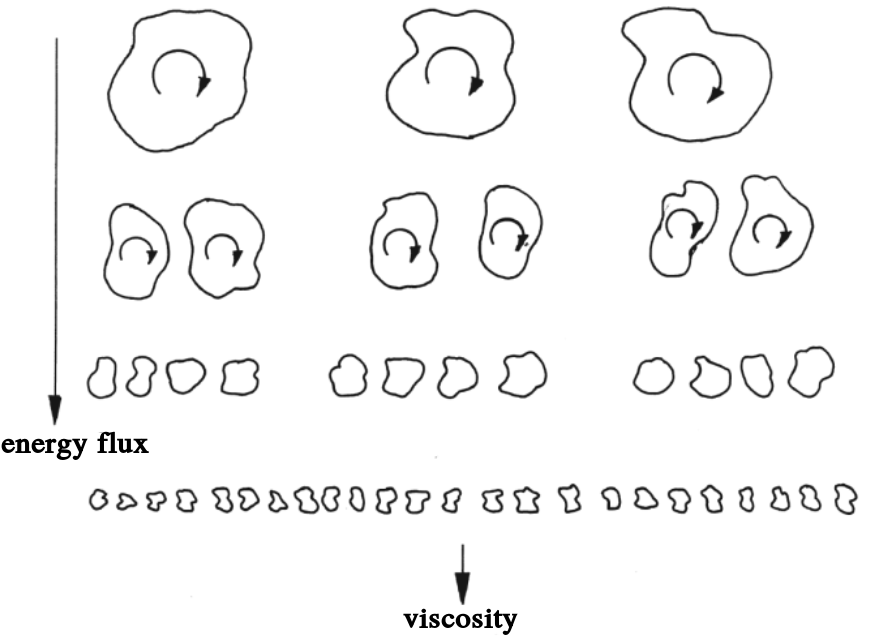
\includegraphics[width=0.75\columnwidth]{./images/probdef/turbulence/energycascade.png}
	\caption{\label{fig:energycascade} Schematic representation of turbulence energy cascade \citep{davidson2015turbulence}, following the sketch by \citet{frisch1995turbulence}.}
\end{figure}

Turbulence is a multi-scale phenomenon, involving scales from the size of the domain till the Kolmogorov dissipative micro-scales. These scales co-exist and interact with each other. Large scales usually contain most of the kinetic energy of the flow, therefore responsible for the transportation of matter, momentum and heat. Small-scale turbulence contains less energy and is strongly involved in the dissipation. Turbulence kinetic energy usually cascades from large to small scales, as schematically represented in figure \ref{fig:energycascade}. The range of scales is continuous, and the width of this range depends on Reynolds number of the flow. 
 
All scales are important to characterize turbulent flows. For instance, an accurate description of all scales is required to estimate full Reynolds stress tensor to validate numerical simulations, turbulence models and scaling theories. This validation is usually performed at very low frequencies, demanding measurements with large field-of-view and long time records. Unsteady flow simulations resolve very small scales in space and time, predict the sharp gradient in the shear layer or near-wall turbulence. Validating these simulations requires small-scale information up to the Kolmogorov length scale.

Small-scale turbulence is crucial to understand the physics of the flow, since they are responsible for the breaking and reconnection of vortices. They are also more likely universal/quasi-universal compared to large scales. A good understanding could lead to turbulence models where the presence of small scales can be parametrized by more universal mathematical models. The efforts to simulate flows could be simplified to large-scale turbulence only, reducing significantly computation costs.  Moreover, small scales are crucial in some contexts such as combustion where matters are brought together at the molecular scales.

\section{Limitations of turbulence research tools}
Despite the constant progress in experiments and numerical simulations, a full access to small-scale turbulence remains impossible for flows at high Reynolds numbers. The section reviews briefly recent advancements and critical limitations. 

\subsection{Numerical simulations}
In academic context, direct numerical simulation (DNS) is the only available tools to directly solve N-S equations without any additional model. It yields all information of the flow via the numerical simulation using an extremely fine grid to resolve all range of scales, from the largest (of the domain size) to the smallest eddies (of the order of the Kolmogorov micro scales). Higher order schemes such as compact finite difference or spectral methods are used to discretize and solve the equations with a very high accuracy.

Constant progress in computational resources permits DNS of higher Reynolds number ($ Re $) and more complex flows. The first attempt of DNS was to simulate isotropic turbulence on a very coarse grid of $ 32^3 $ \citep{fox1972numerical,orszag1972numerical}, while recent simulations of the same flows were performed at $ 4096^3 $ \citep{ishihara2009study,kaneda2003energy}. More complex geometries are also studied, such as channel flows \citep{sillero2013one,lee2014direct}, flat-plate boundary layer under zero and favorable pressure gradients \citep{spalart1986numerical,spalart1988direct} and backward facing step \citep{le1997direct}, among many others.

DNS is limited uniquely to academic context due to computational constraints. The required number of grid points is $ \mathcal{O}\left(Re^{9/4}\right) $ in space and $ \mathcal{O}\left(Re^{3/4}\right) $ in time to resolve the smallest scales. This becomes a real burden for most engineering flows at high $ Re $ and with complex geometries. One of the largest DNS is a channel flow simulation at $ Re_{\tau}\approx 5200 $ \citep{lee2015direct} with the same domain sizes as the well-known simulation by \citet{hoyas2006scaling} at $ Re_{\tau}\approx 2000 $. This is close to $ Re $ of most engineering flows, about $ Re_{\tau}\approx 10^3 $ \citep{smits2013wall}. However, many flows are at $ Re $ one order of magnitude higher and in much more complex geometries. Even when computers become fast enough to simulate those flows, running DNS for engineering flows could produce petabytes of data, which may exceed our capability to analyze and draw useful conclusions.

\subsection{Experimental techniques}
Experiments can provide some information that are not as complete as numerical simulations but for more realistic flows at high $ Re $ and more complex geometries. The most common techniques are hot wire anemometry (HWA) and particle image velocimetry (PIV).

\subsubsection{Hot Wire Anemometry}  
Hot Wire Anemometry (HWA), first proposed by \citet{king1914convection}, is a simple yet accurate technique to measure one-point velocities. The anemometer uses a thin wire at very high temperature submerged into the flow. The flow changes the heat equilibrium around the wire, altering the temperature of the wire. The electronic circuit of the device provide to the wire a controlled amount of electrical current to keep the wire temperature constant. The velocity is deduced from the voltage change. Since the change is analog without any information loss, the temporal frequency of velocity measurements can reach about 100 kHz, which corresponds to Kolmogorov time scale of most realistic flows. The main constraint is the spatial discretization, since only point-wise measurements are possible, and a rake of hot wires soon becomes intrusive.

\subsubsection{Particle Image Velocimetry}  
Particle Image Velocimetry (PIV) is currently the best technique to measure global/topological view of flows. The method aims at recording images of tracers seeded in the flow, which are necessarily light and neutrally buoyant, to measure instantaneous velocity fields \citep{adrian2005twenty,keane1992theory}. Laser light sheets pulsed at a fixed time interval are used to  illuminate a slice of the flow, and pairs of images are recored at the same interval by CCD cameras. Velocity at one point is estimated as the averaged displacement of its neighboring tracers within a so-called ``interrogation window''. The most likely position of a group of tracers inside this window at the next time step is estimated using a correlation technique \citep{sutton1983determination}. Final velocity fields are computed knowing the displacements and the interval between two images of the same pair.

The conventional PIV technique measures two-dimension two-component (2D-2C) velocity fields. \textit{Stereo-PIV (SPIV)} measures two-dimension-three-component (2D-3C) fields \citep{prasad2000stereoscopic}. It uses a system of two synchronized cameras to capture images of a seeded flow. These images are simultaneously taken but with distinct off-axis views so that ``out-of-plane'' velocities can be extracted. These two cameras are usually set up in an angular configuration where the axes of the two cameras are rotated while assuring that they intersect with the object plane along the same axis following the Scheimpflug principle.

\textit{Tomographic PIV} can measure 3D-3C velocity fields. It gives the most complete view of a flow, including the velocity gradient tensor, a crucial measure to validate numerical approaches. Proposed recently by \citet{elsinga2005assessment,elsinga2006tomographic}, the main principles remain analogous to SPIV with important modifications. The illumination of the 3D volume is done with a thicker laser sheet, and 3D velocities are estimated using 3D cross-correlations. Recent measurements can reach 3D-3C fields of a volume of about 200 $ cm^3 $ in water or 50 $ cm^3 $ in air at a frequency of 3 kHz \citep{scarano2013tomographic}. 

\textit{``Shake-The-Box''} (STB) calibration technique aims at improving further the spatial resolution by combining Lagrangian and Eulerian views of a flow. The setup resembles tomographic PIV. The time spacing is required to be of the order of the Kolmogorov time scale to ensure an accurate tracking of particle trajectories. From the time-resolved sequence of tomographic images, STB uses particle image matching to find the Lagrangian trajectory of each particles. Interpolation is used to get velocities on the Euclidean regular grid. This technique ideally reaches the resolution till particle sizes. A recent work using STB permits a resolution of 21 pixels per $ mm^2 $ in a cube of $ 10cm \times 10cm \times 2cm $ at 1 kHZ for a flow at $ Re = 33000$ \citep{schroder2015advances}.

Despite above advancements, PIV is still limited in measuring realistic flows due to optical devices and data processing constraints. The state-of-the-art measurements are still a question of finding compromises among high temporal frequency, high spatial resolution and large field of view. This is due to the following critical limitations. 

The spatial resolution of PIV measurements is limited due to the correlation-based calibration technique. The maximum resolution is constrained by \textit{image density} \citep{keane1992theory}, which is the average number of tracers in an integral window (or interrogation cell). This parameter is very important to determine the measurement quality. Too high image density causes the problem of multiple correlation peaks, while too low image density reduces the possibility to find an image pair for each interrogation window. The optimal choice of image density is about 8-10 tracers per interrogation window, which is a compromise between good spatial resolution and quality of autocorrelation estimate. 

STB can overcome the spatial resolution limits by resolving the fields down to the particle size, but requires a system with a very high sampling frequency. Current PIV systems only reach low frequencies compared to the smallest time scales. State-of-the-art systems can capture up to 10000 frames per second (fps) at a resolution of one mega-pixel \citep{willert2015high}. This fps is very large but still not sufficient for most engineering flows in air. These flows sometimes require measurements at frequencies at least one order of magnitude higher. Moreover, a high speed PIV requires a laser that combines extremely high pulsing frequencies and high power.

\section{Problem definition}
Complete views of turbulent flows at both large and small scales are desired. However, current facilities are not yet available to measure such information. Large-scale  information are gradually available, but small-scale turbulence remains out-of-reach. This work addresses the problem of empirically estimating small-scale information from large-scale measurements. It aims at exploiting available measured data and propose computational methods to reconstruct full fields in new situations. Such methods may permit to go beyond what one can measure, compute or store. The idea of the co-conception approach can be studied, where results from this work potentially paves the way to design experiments or simulations in such way that facilitates the post-processing to recover a maximum level of information.

Though out this thesis, cubic spline interpolation is used to go from low to high resolution. It is used also as the benchmark to compare with the proposed models. Interpolated fields contain no small scales with the frequency higher than the cut-off associated with the grid of measured points, neglecting the aliasing effects due to the subsampling. For this reason, through out this thesis, the term \textit{small-scale} is referred also as \textit{high-frequency} (HF) or \textit{high-resolution} (HR), while \textit{large-scale} has the same meaning as \textit{low-frequency} (LF) or \textit{low-resolution} (LR).

\subsection{Estimating high-resolution turbulent fields from low-resolution measurements}
\label{sec:probdef1}

\begin{figure}
\centering
	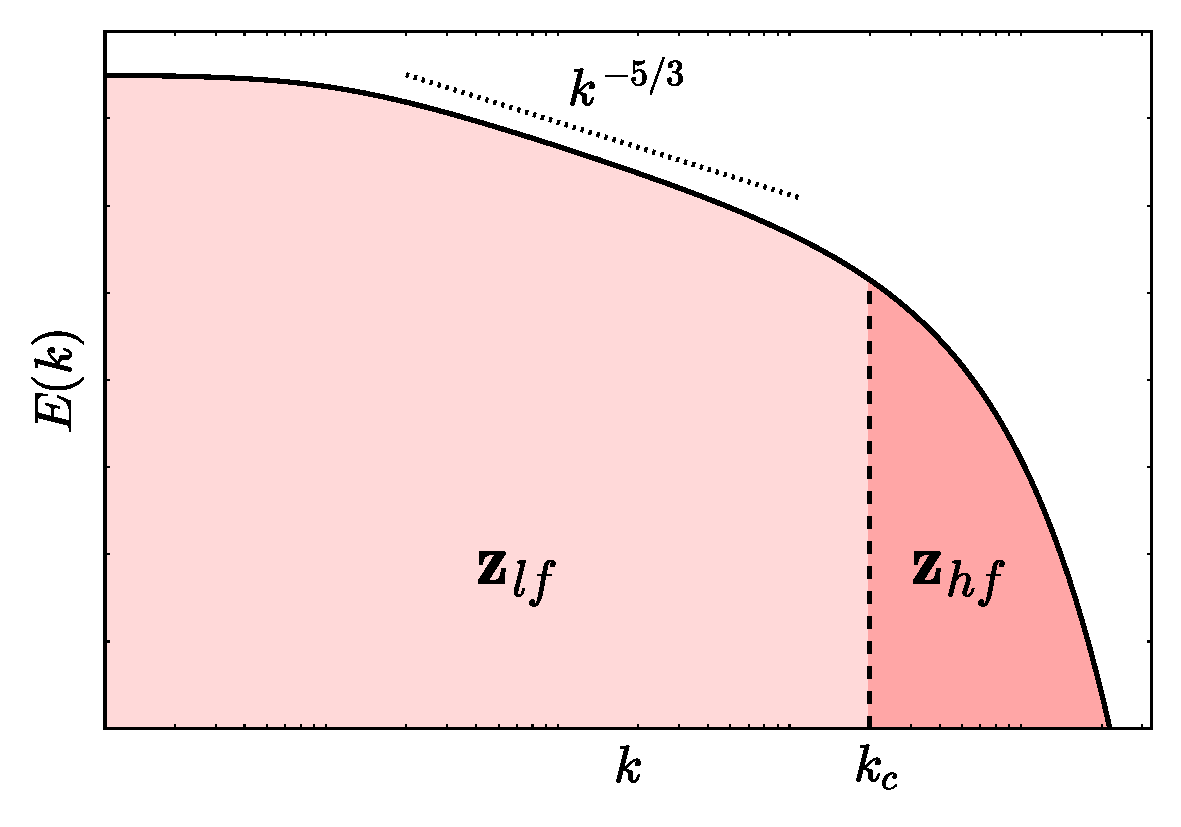
\includegraphics[width=0.6\columnwidth]{./images/probdef/turbulence/turbulence_spectra_long.eps}
	\caption{\label{fig:turbulence_spectra} Turbulence energy spectrum with relative separation between large and small scales by a cutoff wave number $ k_c $.}
\end{figure}

Structures in a turbulent flow can be relatively separated into large and small scales as shown in figure \ref{fig:turbulence_spectra}. Energy content $ E(k) $ is shown as a function of each wave number $ k $ in log-log scale. This Fourier spectrum is continuous, and under certain conditions it has a $ k^{-5/3} $ region. The ranges of scales and their energy contents are very wide depending on $ Re $. Large scales $ \LF $ and small scales $ \HF $ are separated at the cutoff wavenumber $ k_c $. We consider the situation where $ \LF $ - the low spatial resolution or low temporal frequency fields- is measured while $ \HF $ is not accessible. 

The question is \textit{can small scales be estimated from large-scale measurements}? This can be considered as whether a mapping function $ f $ exists such that, given LF measurements, the HF contents $ \HF $ of the flow can be predicted by:
\begin{equation}
f:  \LF \mapsto  \HFest  = f \left(\LF\right)
\end{equation}
No theoretical mapping function exists, although turbulent flows are governed by N-S equations. Despite constant attempts, researchers have not succeeded in proposing turbulence models to represent universal relations between large and small scales.

This thesis aims at proposing empirical functions, either linear and nonlinear, to estimate small-scale information given the large scales. The use of ``empirical'' models is in the sense of learning, where data at all scales are available \textit{a priori}. The proposed algorithms learn from the training data a empirical relation between large and small scales. This relation is presented in the form of a function $ f(.) $, which permits to estimate small-scale information in new situations.

\begin{figure}
\centering
	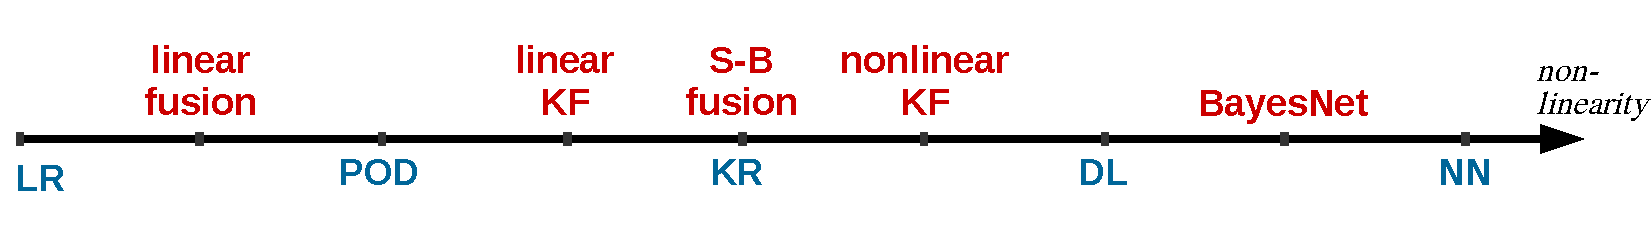
\includegraphics[width=\columnwidth]{./images/probdef/turbulence/models_spectrum.pdf}
	\caption{\label{fig:models_spectrum} Spectrum of models ordered by their level of nonlinearity (from left to right). Methods for mapping large-small scales are in blues, while those for fusion of measurements are in reds. Notations: linear regression (LR), proper orthogonal decomposition (POD), Kalman filter (KF), kernel regression (KR), similarity-based (S-B), dictionary learning (DL), Bayesian network (BayesNet), neural network (NN).}
\end{figure}

A large spectrum of methodologies is discussed and compared. Figure \ref{fig:models_spectrum} lists such methods (in blue) as a function of the order of their nonlinearity. Pure linear models are conventional regression and dimensionality reduction (POD)-based methods. Nonlinearity level grows with model complexity. Simple nonlinear models, the so-called kernel regression, work in a fixed kernel space. The family of dictionary learning methods provides sparse representation of high dimensional data. Neural network, a broader and very active research field, finds nonlinear mapping functions with a more adaptive kernel space. A ``deep'' network permits to model highly nonlinear phenomena. However, we will leave this approach for future works.

\subsection{Fusion of large-scale measurements}
\label{sec:probdef2} 
Turbulence is multi-scale both in space and in time. Usually large or small scales refer to either space (up to three dimensions) or time. However, LF measurements in space potentially contain some HF information in time and vice-versa. One idea is to measure those LF information by different measurement techniques and combine them to infer some HF contents. Such a fusion model takes benefit from each measurement by capturing all possible detailed information. The fused fields contain some small scales that are not accessible from each single measurement. 

\begin{figure}
\centering
	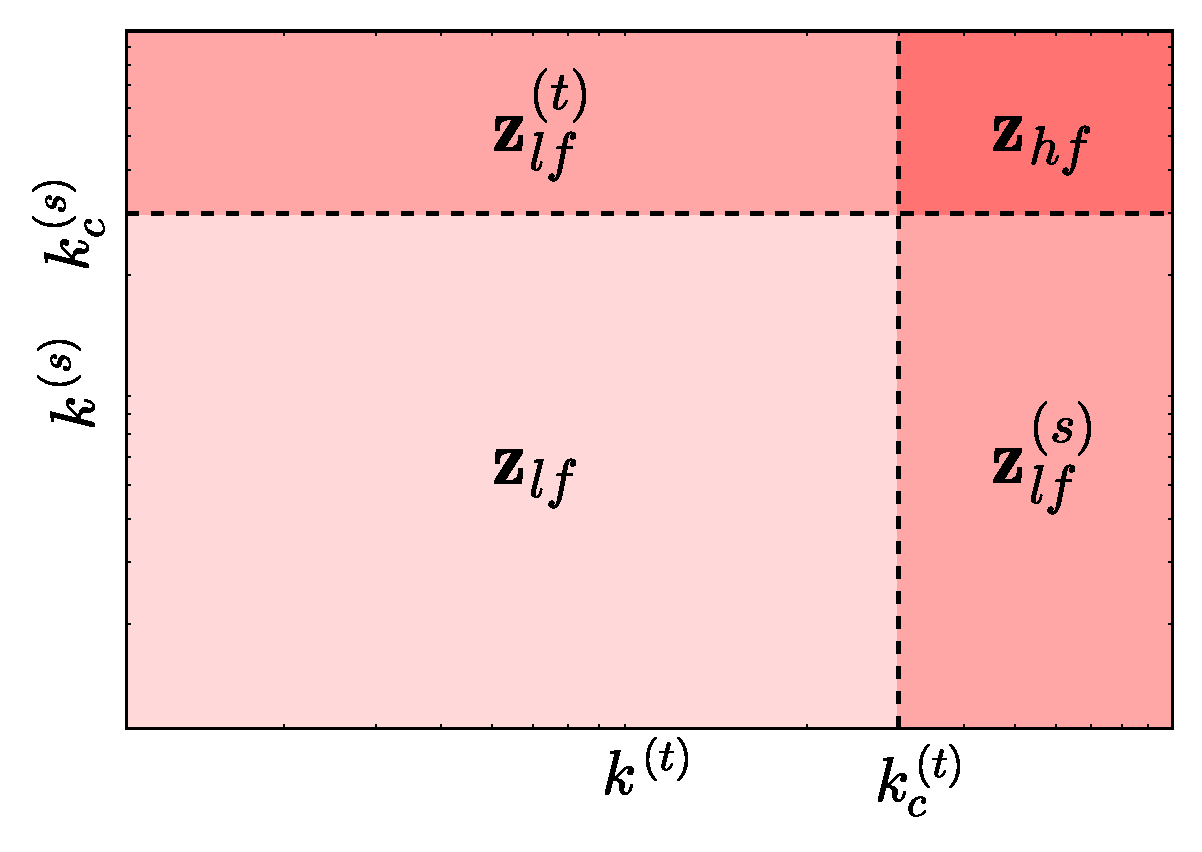
\includegraphics[width=0.5\columnwidth]{./images/probdef/turbulence/space_time_wavedomain_long.eps}
	\caption{\label{fig:space_time_wavedomain} Turbulence energy spectrum with relative separation between large and small scales at wave number $ k_c $.}
\end{figure}

Figure \ref{fig:space_time_wavedomain} depicts schematically the above idea, where LF measurements in space and time are illustrated. In space, two sources of information $ \left\lbrace \LF, \LF^{(s)} \right\rbrace$ are available, where $ \LF $ contains purely LF information in space-time, and $ \LF^{(s)} $ captures LF in space but over the full range of temporal frequencies. An analogous interpretation is for $ \left\lbrace \LF, \LF^{(t)} \right\rbrace $ in time, where $ \LF^{(t)} $ potentially gives some detailed information of the flow in space. By combining two sources of LF measurements in space and time, ideally one can hope to predict all scales in three blocks $ \LF $, $ \LF^{(t)} $ and $ \LF^{(s)} $, while those within $ \HF $ are unreachable. 

\begin{figure}
\centering
	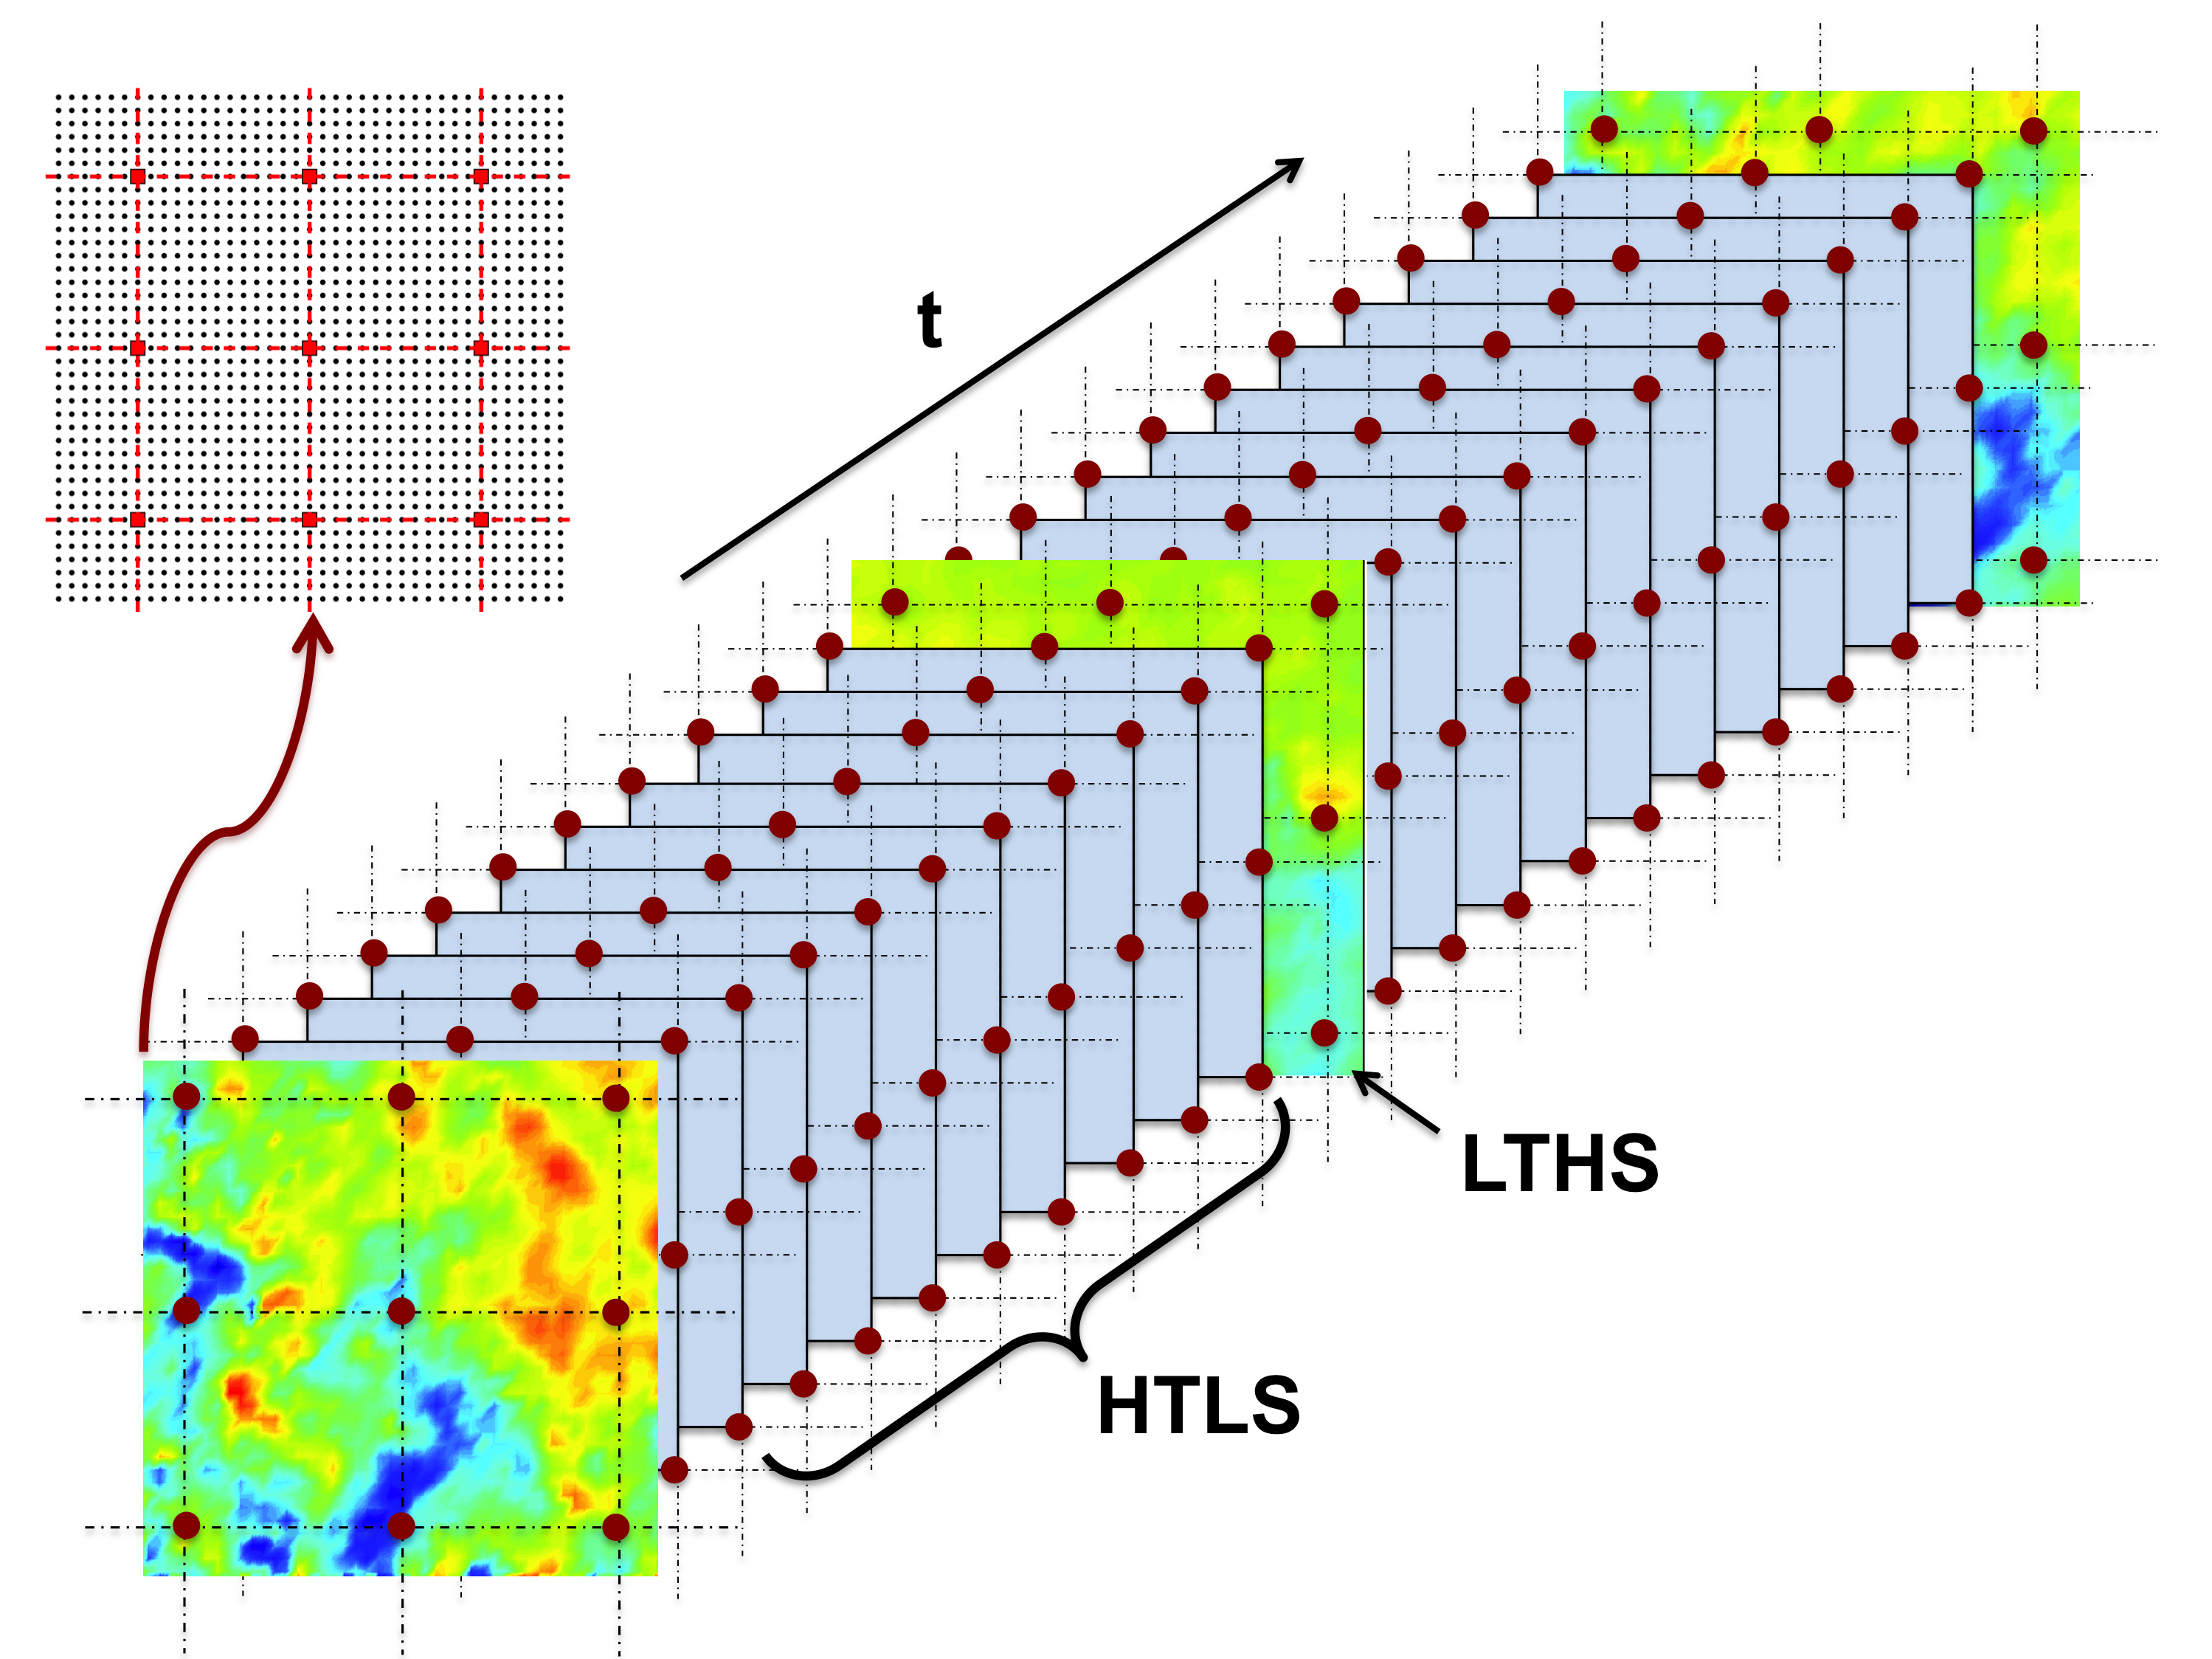
\includegraphics[width=0.5\columnwidth]{./images/probdef/setups/problem_config.png}
	\caption{\label{fig:space-time_measurements} Sketch of the inverse problem, with the two sources of measurements: the LTHS (color images) and a coarse grid of HTLS (red dots among black ones of LTHS). The inverse problem of HTHS data reconstruction is to fill in the space-time data-cube.}
\end{figure}

This work addresses a configuration as in figure \ref{fig:space-time_measurements} where two sources of measurements, the high-temporal-low-spatial (HTLS) and low-temporal-high-spatial (LTHS) resolution velocity fields are available. LTHS measurements (black dots) at the three colorful planes are synchronized with HTLS measured positions at LR (red dots). HTLS captures HF contents of the flow dynamics, while LTHS measures highly resolved information in space. By combining these two sources, one hopes to capture more small-scale information in space and time. 

This idea has been studied at LML in an European joint experiment \citep{coudert2011double}. A database of a boundary layer flow at high $ Re $ was measured using SPIV synchronized with a rake of HWA probes. PIV measurements (LTHS) are with a large field-of-view ($ 30 \times 30 cm $) and a high spatial resolution ($ 143 \times 167 $) but at a low acquisition frequency ($ 4 Hz $). HWA measurements in a rake of probes (HTLS) of the same field-of-view are sampled at an extremely high rate ($ 50 kHz $). However, the spatial discretization is very coarse ($ 11 \times 13 $) compared to the smallest scale. The post-processing step is to estimate velocity fields at the frequency $ 50 kHz$ and the resolution $ 143 \times 167 $.

This work studies computational methods to combine HTLS and LTHS measurements to maximize the information level. The spectrum of possible methods as the order of nonlinearity is shown (in red) in figure \ref{fig:models_spectrum}. For completeness, the idea of data assimilation using linear/nonlinear Kalman filter is mentioned, but further discussion is outside the scope of this work. A fusion approach based on local similarity, the so-called similarity-based (S-B) scales propagation model, is proposed. This method further exploits the local information of the flow, with certain advantages and limitations compared to the linear fusion model. Another fusion method based on Bayesian framework is also proposed, which is further simplified as a linear model.

\section{Datasets}
Experimental data are available from the WALLTURB project \citep{coudert2011double}. However, there is no HR reference data in space-time to qualify and compare different reconstructions. This is the reason why DNS data are used in the present study to access fully resolved velocity fields. Data acquire the true properties of turbulent fields, since DNS simulates flows without any turbulence modeling. The data are also free from measurement uncertainties and noises, making possible a fair comparison of different models. LR measurements are virtually extracted from HR data. The proposed models are learned from these training data to reconstruct fully resolved fields, which are used to estimate the accuracy of different approaches by comparing to reference DNS data.

Two DNS datasets are used . The first data is from the DNS of a turbulent channel flow at a moderate $ Re $. The designed numerical experiments on this data very well imitate the database from LML experiment. However, due to the problem of non-homogeneity, it is challenging for some models to perform. Data of isotropic turbulence is used as well, with further assumptions of isotropy, periodicity and homogeneity, but still retains the principal properties of turbulence.

For both data, the configuration of HTLS and LTHS measurements as in figure \ref{fig:space-time_measurements} is studied, with the following notations to describe. HTHS, HTLS and LTHS snapshots at the $ t-$th time step are denoted as $ \z_t \in \R^{\dimsh} $, $ \y_t \in \R^{\dimsl} $ and $ \x_t \in \R^{\dimsh} $, respectively. The dimension of HR fields ($ \z_t $ and $ \x_t $) is $ \dimsh $, higher than the LR dimension $ \dimsl $ of $ \y_t $. There are $ \dimth $ HTHS and HTLS snapshots, and only $ \dimtl $ LTHS ones ($ \dimtl < \dimth $) sampled at $ t=1,1+1 \times \dimth/\dimtl,1+2 \times \dimth/\dimtl,...,1+(\dimtl-1)\times \dimth/\dimtl $. The matrix form of $ \{\z_t\} $, $ \{\y_t\} $ and $ \{\x_t\} $ are $ \Z $, $ \Y $ and $ \X $ of sizes $ \dimth \times \dimsh $, $ \dimth \times \dimsl $ and $ \dimtl \times \dimsh $ respectively. 

\begin{figure}[t]
\centering
	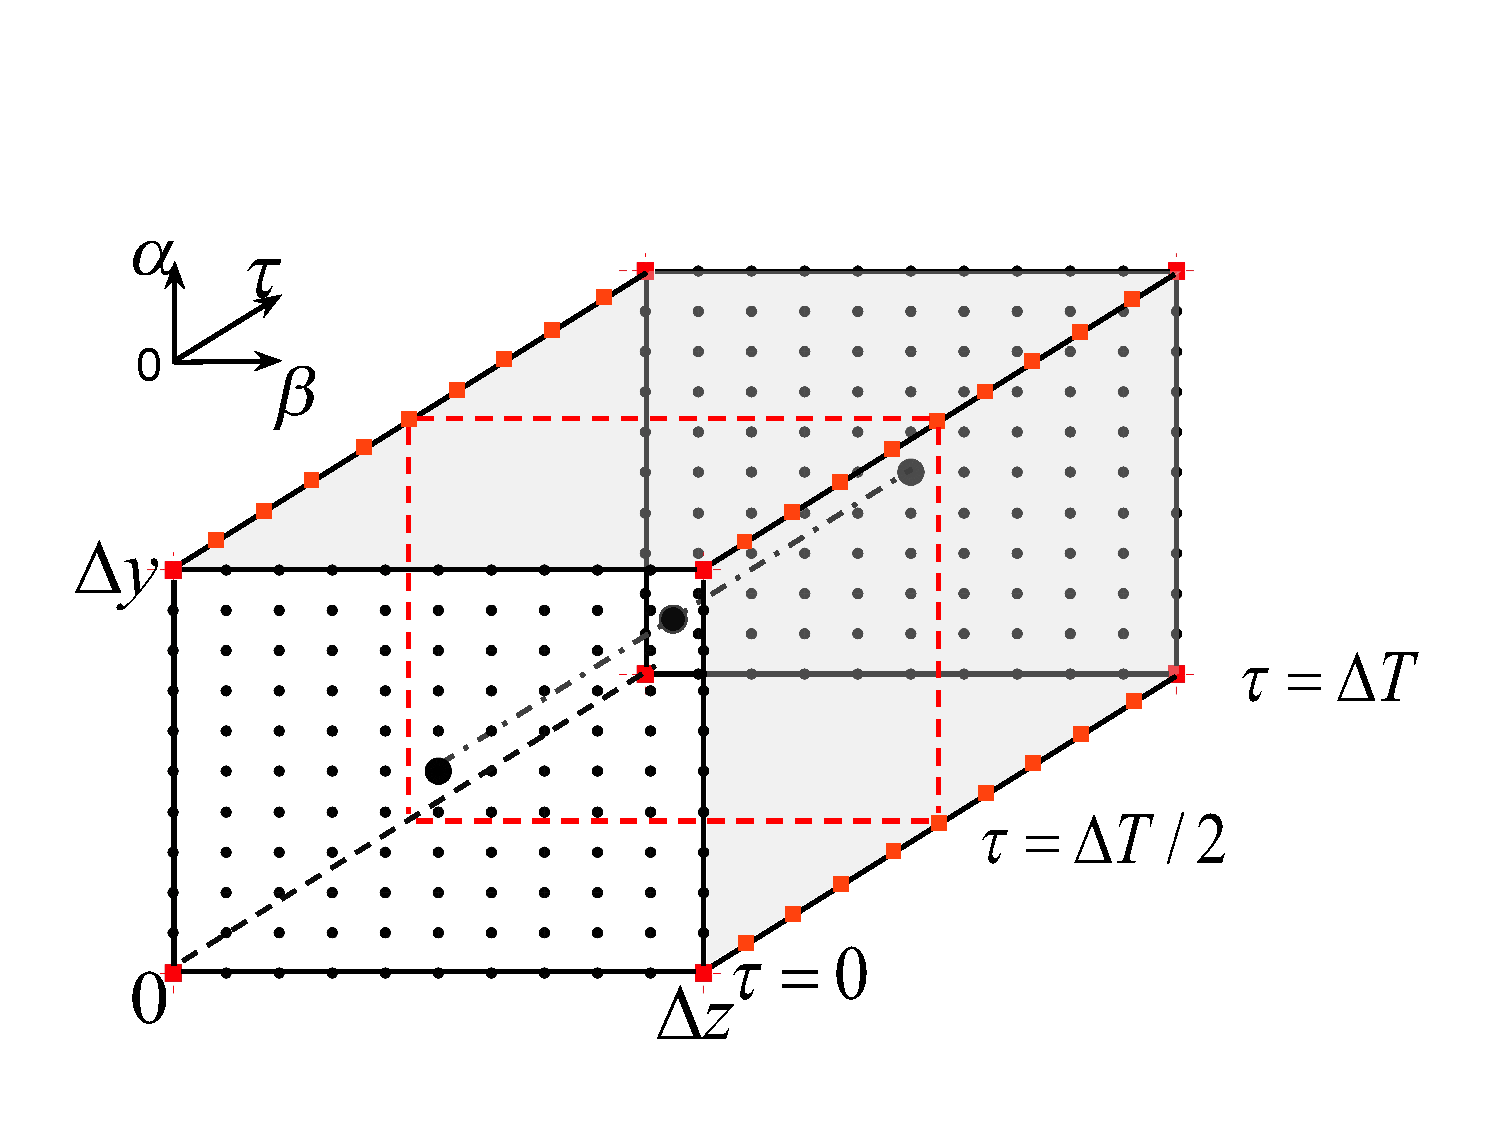
\includegraphics[width=0.6\columnwidth]{./images/probdef/setups/element_block.pdf}
	\caption{\label{fig:element_block} Sketch of an element block with local coordinates $ (\alpha,\beta,\tau) $. LTHS time steps are at $ \tau/\delta t=0 $ and $ \tau/\delta t=\dimth/\dimtl $. HTLS measurements are represented by red dots and LTHS measurements by black ones. }
\end{figure}

To describe all numerical experiments, it is useful also to introduce a sketch of an \textit{element block} bounded by the measurements as in figure \ref{fig:element_block}. This sketch is also used later to characterize performances of all models, since reconstruction accuracies depends on the relative positions in this block. A local coordinate system is introduced. The time position $ \tau $ is defined as a relative distance to two bounded LTHS snapshots (black dots) at $ \tau =0 $ and $ \tau = \Delta T = \dimth\delta t/\dimtl  $ ($ \delta t $ is the time distance between two neighboring HTLS planes). In space, each plane at $ \tau $ is bounded by the four HTLS measurements at the four corners (red points). The distances between two neighbors are $ \Delta y  = \delta y\sqrt{\dimsh/\dimsl} $ in vertical and $ \Delta z = \delta z\sqrt{\dimsh/\dimsl} $ in spanwise direction. $ \delta y $ and $ \delta z $ are spatial grid sizes in vertical and spanwise direction respectively. We assumed also the sampling ratio are equally $ \sqrt{\dimsh/\dimsl} $ in both directions. The most difficult positions to estimate are at local coordinate $ (\alpha, \beta, \tau) = (\Delta y/2,\Delta z/2,\Delta T/2)  $.

The following parts describe the two datasets in detail.

\subsection{DNS data of channel flow}
\label{sec:data_channel} 
\begin{table}
	\caption{\label{tab:energyloss_chanel}
	Configuration parameters of three subsampling cases in space and three in time for DNS channel flow data. The subsampling ratios of HTLS measurements are $ \sqrt{\dimsh /\dimsl } $ and equal in both spatial directions. The ratios of LTHS measurements in time are $ \dimth/\dimtl $. The equivalent spacing in spanwise direction is normalized by half channel height as $ \Delta z/H $ and the spacing in time is $\Delta t$. The normalized energy losses in space $\Delta\kappa_s$ and in time $\Delta\kappa_t$ are defined in equation \ref{eq:RMS_losses}.}
	\vspace{.5cm}
	\centering
	\begin{tabular}{lcS[table-format=1.2]S[table-format=1.2]S[table-format=1.2]cS[table-format=1.2]S[table-format=1.2]S[table-format=1.2]} 
		\toprule
		& & \multicolumn{3}{c}{Space} & & \multicolumn{3}{c}{Time} \\
		\cmidrule{1-1} \cmidrule{3-5} \cmidrule{7-9} 
		Subsampling ratio &  & 5  & 10 & 20 & & 4 & 10 & 20\\ %\addlinespace
		Spacing &  & 0.05  & 0.11 & 0.22 & &  0.10 & 0.25 & 0.50\\ %\addlinespace
		\myrowcolour
		Energy loss $\Delta\kappa$ $ (\%) $ &  & 1.23  & 7.08 & 20.83 & & 01.88 & 9.02 & 24.31 \\ %\addlinespace
		\bottomrule
	\end{tabular}
\end{table}

\begin{figure}[t]
	\centering
	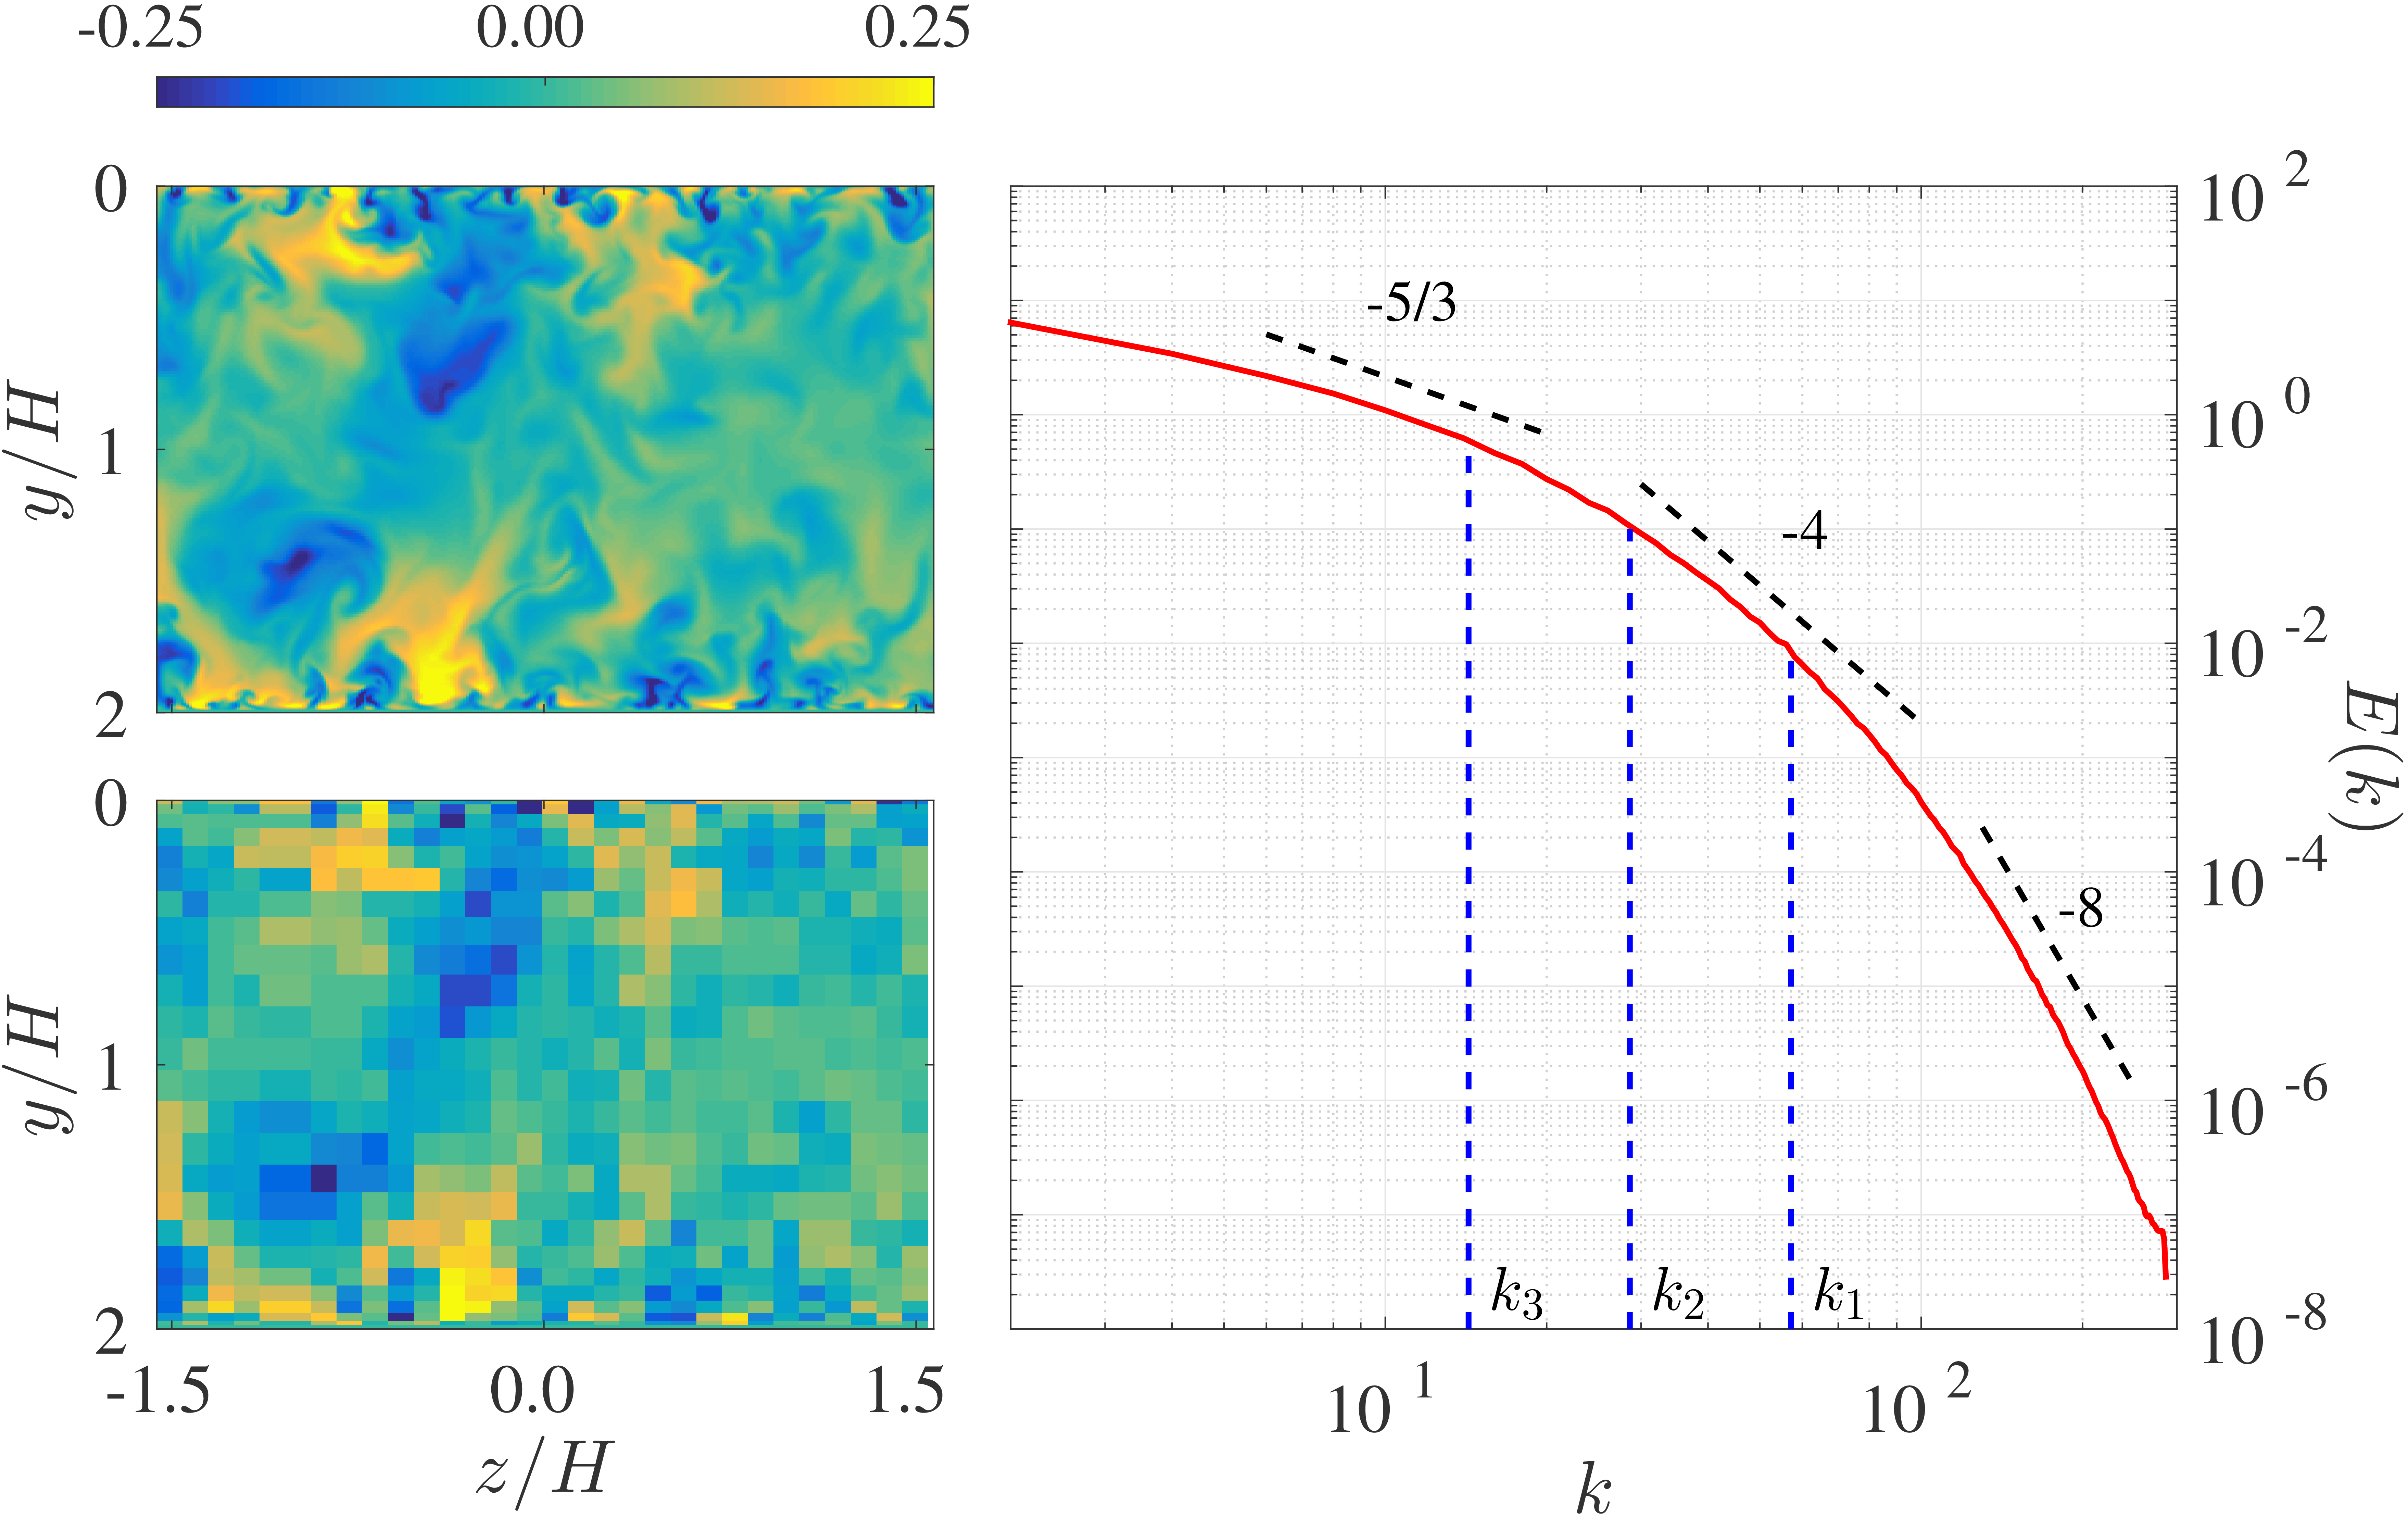
\includegraphics[width=\columnwidth]{./images/datstats/channel/samplevels_spectrum_spanwise_refDNS.png}
	\caption{\label{fig:channel_samplesnap_2D} A sample 2D streamwise velocity of simulated channel and its subsampled field by a factor of 10 (left). This subsampling ratio corresponds to the cut-off wave number $ k_2 $in the plot of spectrum (right) for horizontal lines at the center of the channel. Other wave number $ k_1 $ and $ k_3 $ correspond to the subsampling ratio in space of $ 5 $ and $ 10 $ respectively. }
\end{figure}

DNS database of a turbulent wall-bounded flow is designed the same way as experimental ones. The simulation uses the numerical procedure described in \cite{marquillie2008direct}.
The flow is at a Reynolds number $ Re_{\tau}=550 $ based on the friction velocity $ u_{\tau} $. Cartesian coordinates of the simulation in space are $ (x,y,z) $ for streamwise, vertical and spanwise directions respectively. The domain size normalized by half the channel height $ H $ is $ 2\pi \times 2 \times \pi $. Fully resolved fluctuating streamwise velocities in a plane normal to the flow direction are considered as HTHS data. This data includes $ \dimth=10000 $ snapshots over a grid of $ \dimsh = 288 \times 257 $ points and at a sampling frequency of $ f=\frac{H}{\delta t U_{max}} = 40 $, subsampled from the original simulation at $ f = 200  $. $ U_{max} $ is the central velocity of the flow. LTHS and HTLS measurements subsampled from HTHS data are used to train different prediction models. HTHS is used as the ground truth to estimate reconstruction errors. The extension to spanwise and vertical velocity components follows the same procedure.

Various subsampling ratios both in space and time are considered. In space, the LR fields are obtained by applying a direct subsampling ratio of $ \sqrt{\dimsh /\dimsl } = 5, 10 $ or $ 20 $ in both spatial directions. These ratios correspond to a number $ \dimsl  $ of virtual HTLS sensors of $ 51 \times 57 $, $ 26 \times 29 $ and $ 13 \times 15 $ respectively. Each ratio has a spacing between two successive HTLS points in spanwise and vertical directions of $ \Delta z $ and $ \Delta y $. To test the idea of combining space-time sparse measurements, these subsamplings in space are used together with subsamplings in time of ratios $ \Delta T = \dimth/\dimtl = 4, 10$ or $ 20 $, corresponding to the total number of snapshots $ \dimtl  = 2500, 1000 $ and $500 $ respectively. Each ratio, both in space and time, corresponds to a certain amount of kinetic energy loss. This is essentially the energy of small scales separated from the large ones by a low pass filter (LPF) $ \LPF $. In practice $ \LPF $ will be the $ 5^{th}-$order least square spline filter, either 1D in time ($ \LPF_t $) or 2D in space ($ \LPF_s $), using measurements as knots. This spline filter has the advantage of a sharp cutoff response with a finite support. The energy loss is defined by comparing the filtered field $ \LPF\z  $ to the original field $ \z  $: 
\begin{equation}
	\Delta\kappa=\frac{\displaystyle \sum\limits_{j\in \varmathbb{J}} \z _j^2-\sum\limits_{j\in \varmathbb{J}}{[\LPF\z ]_j^2}}{\displaystyle \sum\limits_{j\in \varmathbb{J}}\z _j^2}
	\label{eq:RMS_losses}
\end{equation} 
where $ \varmathbb{J}$ is the considered set of points. Table~\ref{tab:energyloss_chanel} gathers the energy loss in time ($ \Delta\kappa_t $) and in space ($ \Delta\kappa_s $) estimated with $ \LPF_t $ and $ \LPF_s $ respectively. The set $ \varmathbb{J}$ here contains all points at the center line of the channel, i.e. $ y/H=1 $.

\subsection{DNS data of isotropic turbulence}
\label{sec:data_isotropic}
\begin{figure}[t]
	\centering
	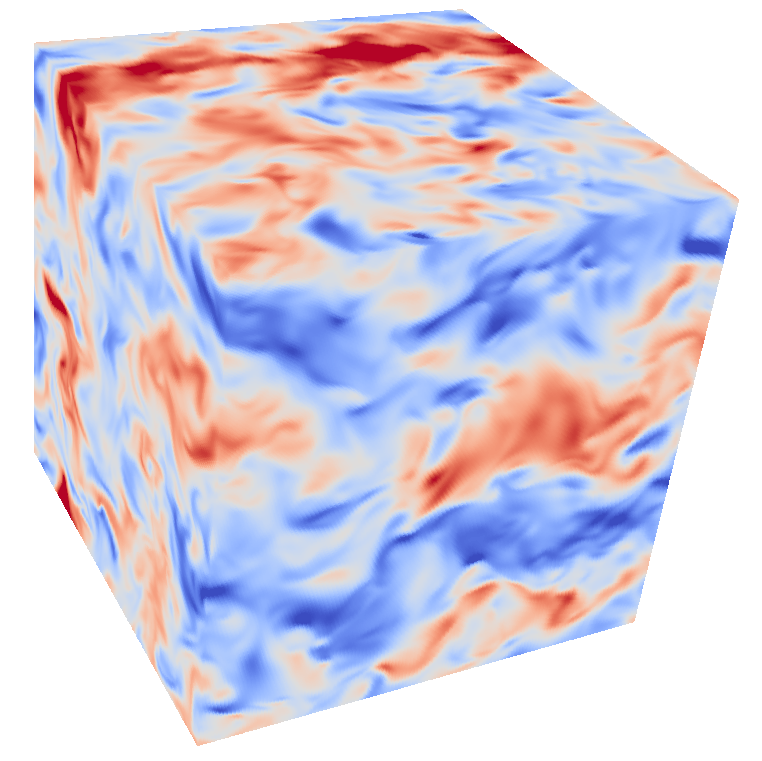
\includegraphics[width=0.45\columnwidth]{./images/datstats/isotropic/velocity_x_3D.png}
	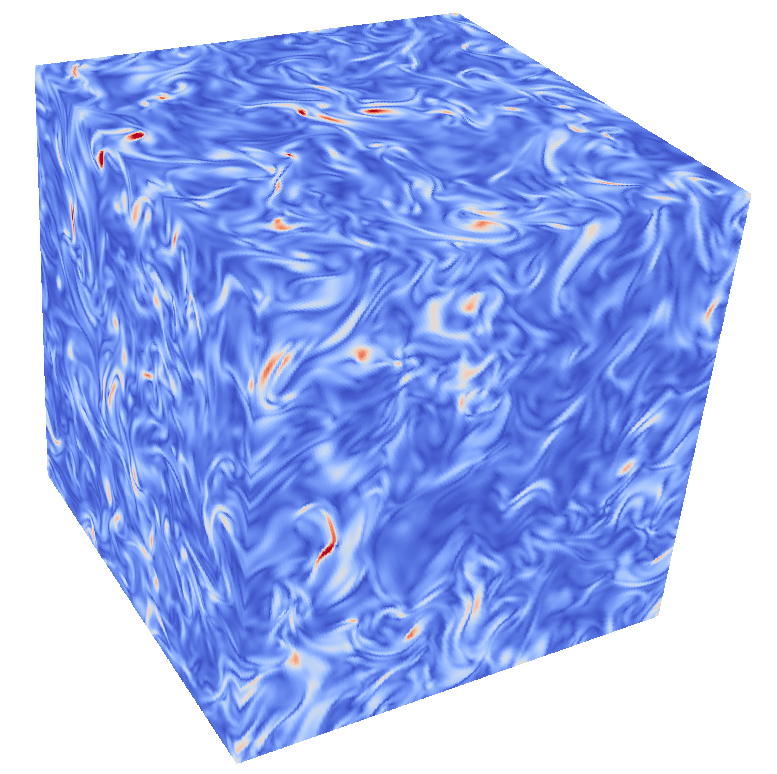
\includegraphics[width=0.45\columnwidth]{./images/datstats/isotropic/vortices3D.png}
	\caption{\label{fig:vortices3D} A sample 3D streamwise velocities (left) and vortices magnitude (right) of DNS isotropic turbulence at $ 384^2 $. The streamwise direction is considered as ``time'' dimension in this case. }
\end{figure}

Channel flows with strong nonhomogeneity in vertical direction yields varying statistics in this direction. Numerical tests of different methods and comparisons of results are more challenging. This nonhomogeneity also calls for a very large database, since all the averaging can be done only in spanwise direction (roughly at the center of the channel) and time. The DNS database of \textit{homogeneous isotropic turbulence} is used for simplifications yet retaining essential properties such as three-dimensionality, intermittency and multi-scale vortices. This flow is assumed to be incompressible inside a periodic box with nearly homogeneous and isotropic statistics. The data are recorded from a simulation over a $ 384^3 $ grid using the Fourier spectral method as originally proposed by \citet{orszag1972numerical}. Figure \ref{fig:vortices3D} shows a sample of a 3D streamwise velocity and vorticity magnitude. $ Re $ is relatively low compared to the state-of-the-art  $ 4096^3 $ simulations by \citep{kaneda2003energy,ishihara2009study}. However, for the purpose of this work, the position of the cut-off frequency is the key parameter and the width of the inertial range is not crucial. Reconstruction accuracy is expected to depend more on the energy loss due to subsampling rather than on $ Re $. Also, the accuracy depends on the slope of the energy spectra at the cut-off frequency, which represents the physics of the flow and implies the level of correlation between neighboring scales

A total of 37 blocks of 3D fields at resolution $ 384^3 $ is recorded. Since a long record of time-resolved data is not available, the streamwise direction is virtually considered as the ``time'' dimension to homogenize the notations for the two datasets. These data are then downsampled by a factor of 4 in every dimension using an ideal Fourier filter, resulting in 3D fields on a $ 96^3 $ grid. The objective is to avoid working within the dissipative range where energy content is very low, leading to a too small energy loss for a given subsampling ratio. Also, the slope of the spectrum is rather high, implying very weak level of correlation between the measured scales and the ones to be reconstructed. Only a small subsampling ratio will now lead to a significant loss, therefore avoiding to work with large ratios and corresponding large numbers of uncertainty. The cubes of $ 96^3 $ are now considered as the reference HTHS fields. Only streamwise velocities in a plane normal to the flow direction are extracted. LR fields will be obtained by virtually subsampling from reference HR ones. A completely analogous procedure is applied to other velocity components.

\begin{figure}[t]
	\centering
	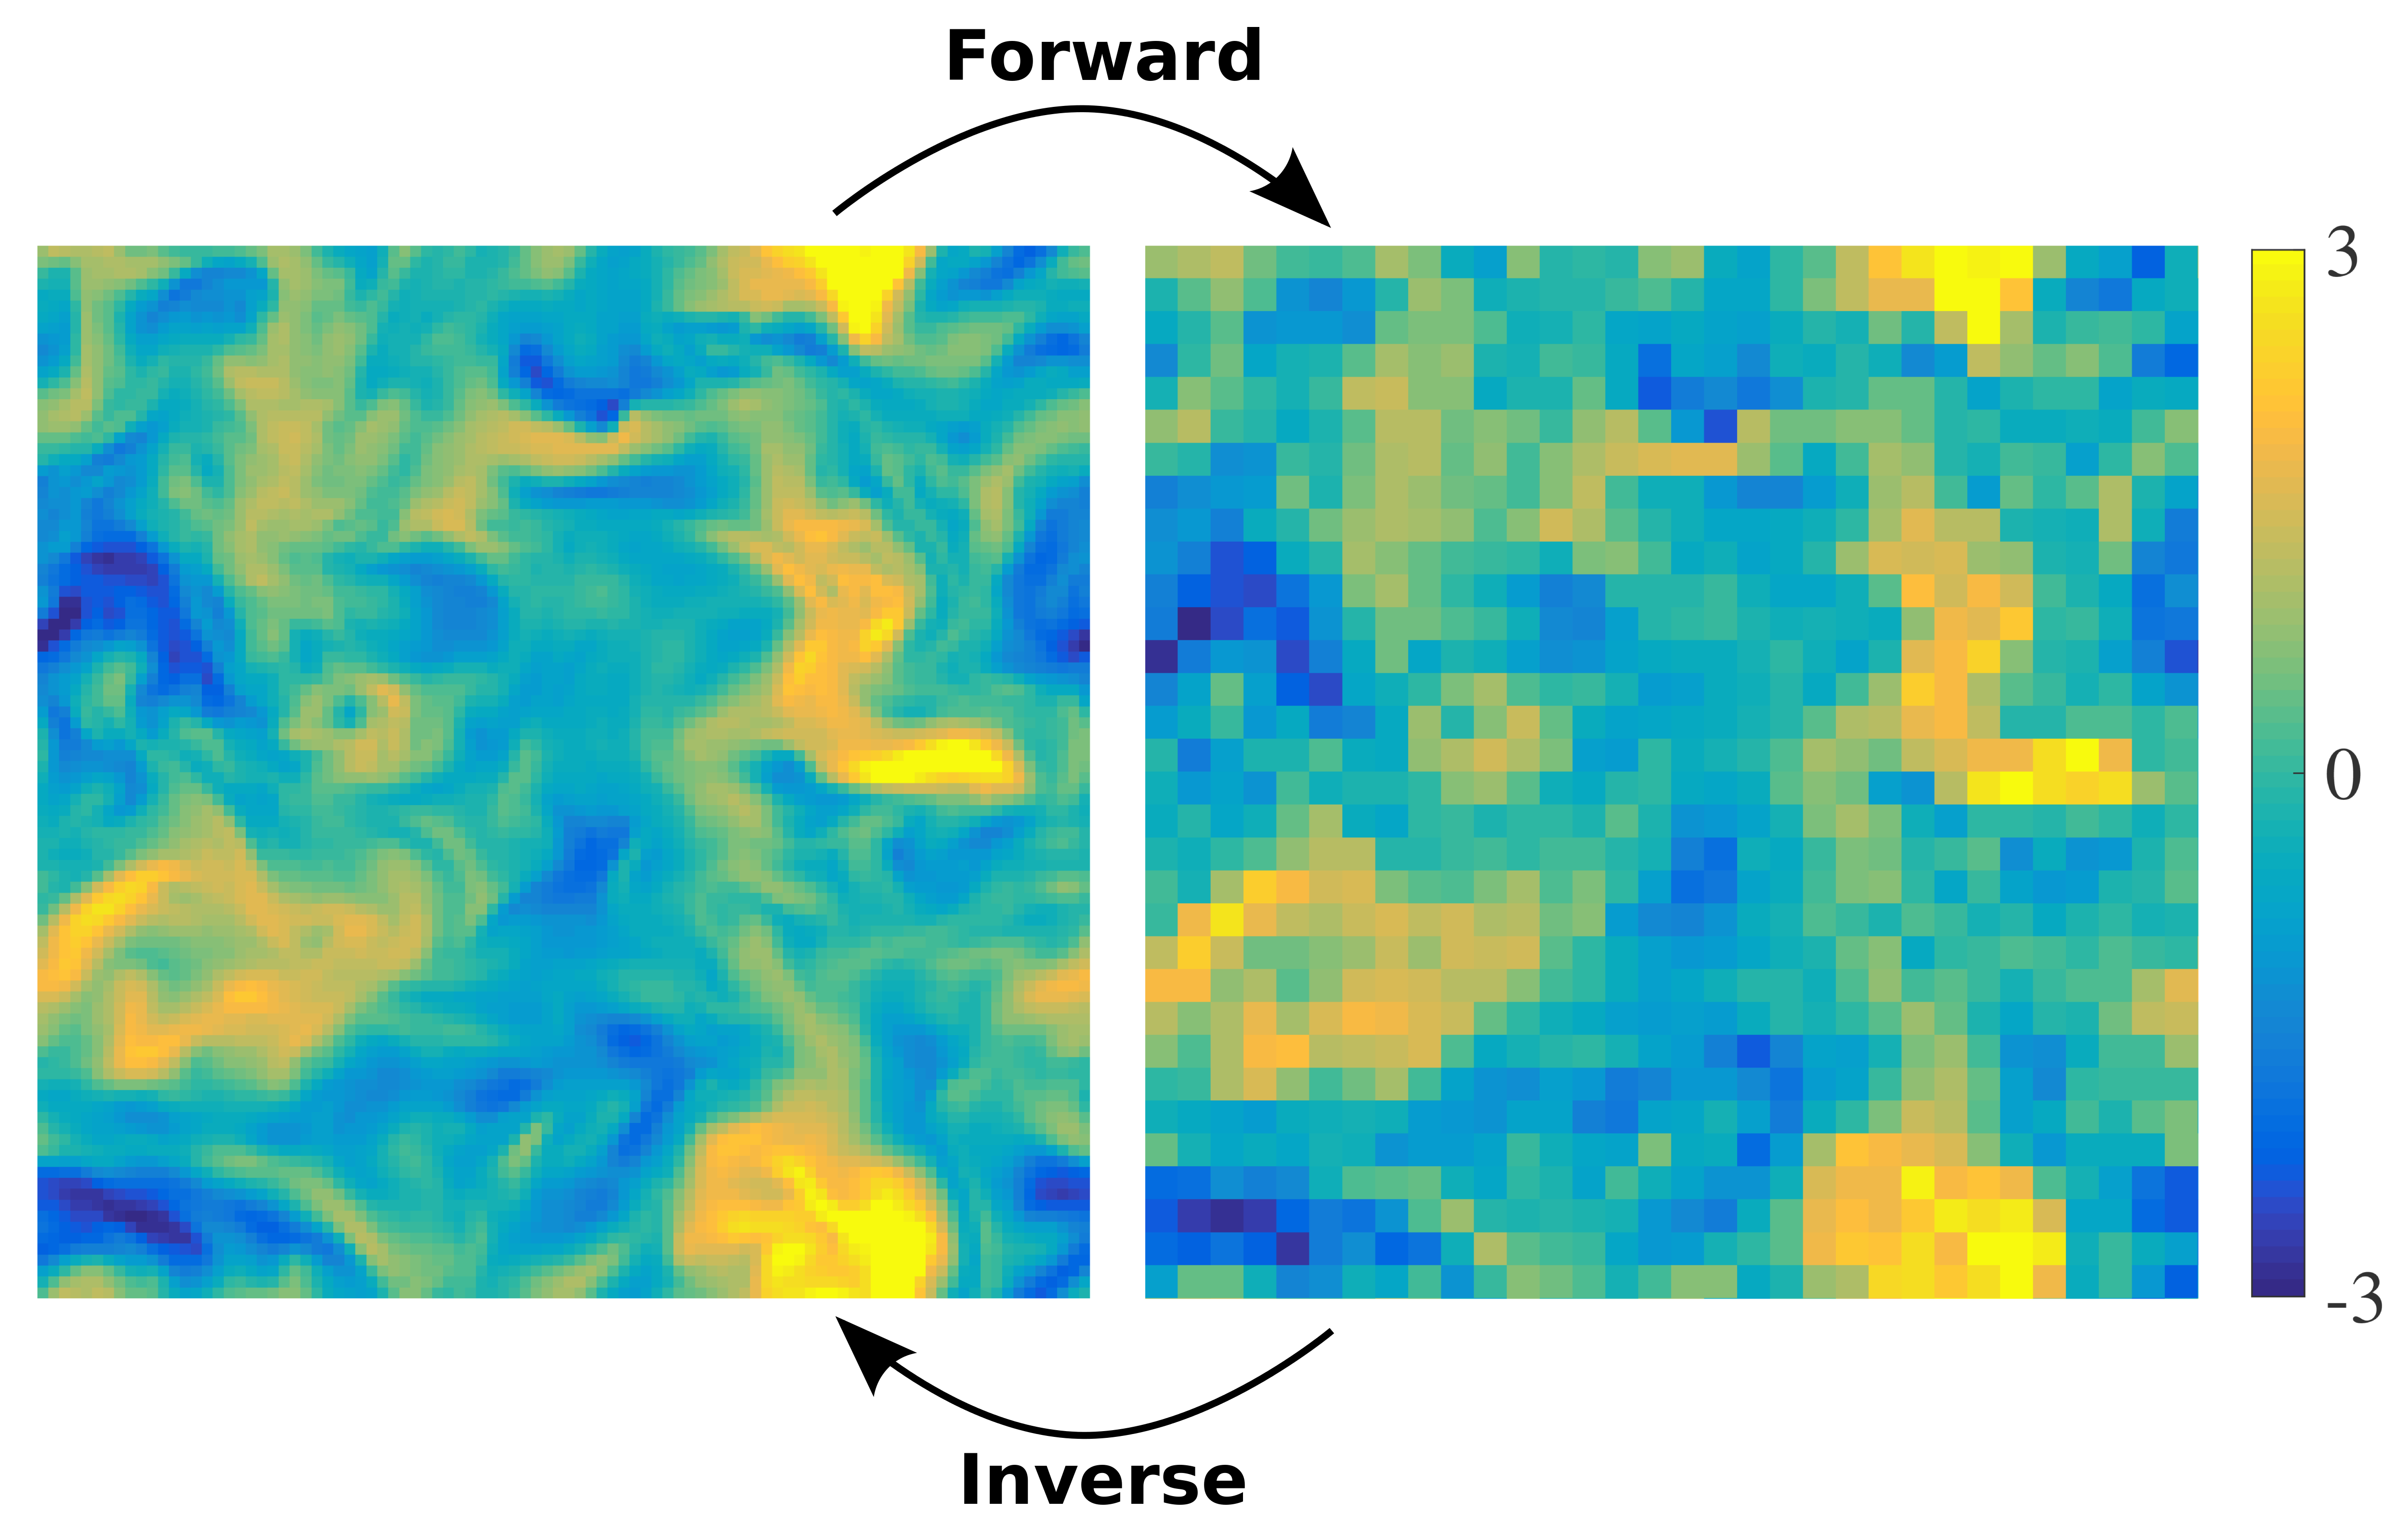
\includegraphics[width=0.8\columnwidth]{./images/datstats/isotropic/u_HR_2D_2.png}
	\caption{\label{fig:u_HR_2D} A sample isotropic 2D streamwise velocity (left) and its subsampled field by a factor of 3 (right) on the plane normal to flow direction. The subsampling is a forward problem, while going from a subsampled to fully-resolved field is an inverse problem.}
\end{figure}

\begin{table}
	\caption{\label{tab:energyloss_isotropic}
		Configuration parameters of three subsampling cases in space (spanwise+vertical direction) and three in time (streamwise direction) for isotropic turbulence data. The subsampling ratios of HTLS measurements are $ \sqrt{\dimsh /\dimsl } $ and equal in both spatial directions. The ratios of LTHS measurements in time (spanwise in this case) are $ \dimth/\dimtl $. The normalized energy losses in space $\Delta\kappa_s$ and in time $\Delta\kappa_t$ are defined in equation \ref{eq:RMS_losses}. The slopes are purely to qualify the steepness of the spectrum and have no physical meaning.}
	\vspace{.5cm}
	\centering
	\begin{tabular}{lcS[table-format=1.2]S[table-format=1.2]S[table-format=1.2]cS[table-format=1.2]S[table-format=1.2]S[table-format=1.2]} 
		\toprule
		& & \multicolumn{3}{c}{Space} & & \multicolumn{3}{c}{Time} \\
		\cmidrule{1-1} \cmidrule{3-5} \cmidrule{7-9} 
		Subsampling ratio &  & 3  & 4 & 6 & & 4 & 6 & 8\\ %\addlinespace
		\myrowcolour
		Energy loss $\Delta\kappa$ $ (\%) $ &  & 1.03  & 2.63 & 7.29 & & 1.23 & 3.56 & 6.53 \\ %\addlinespace
		\bottomrule
	\end{tabular}
\end{table}

\begin{figure}[t]
	\centering
	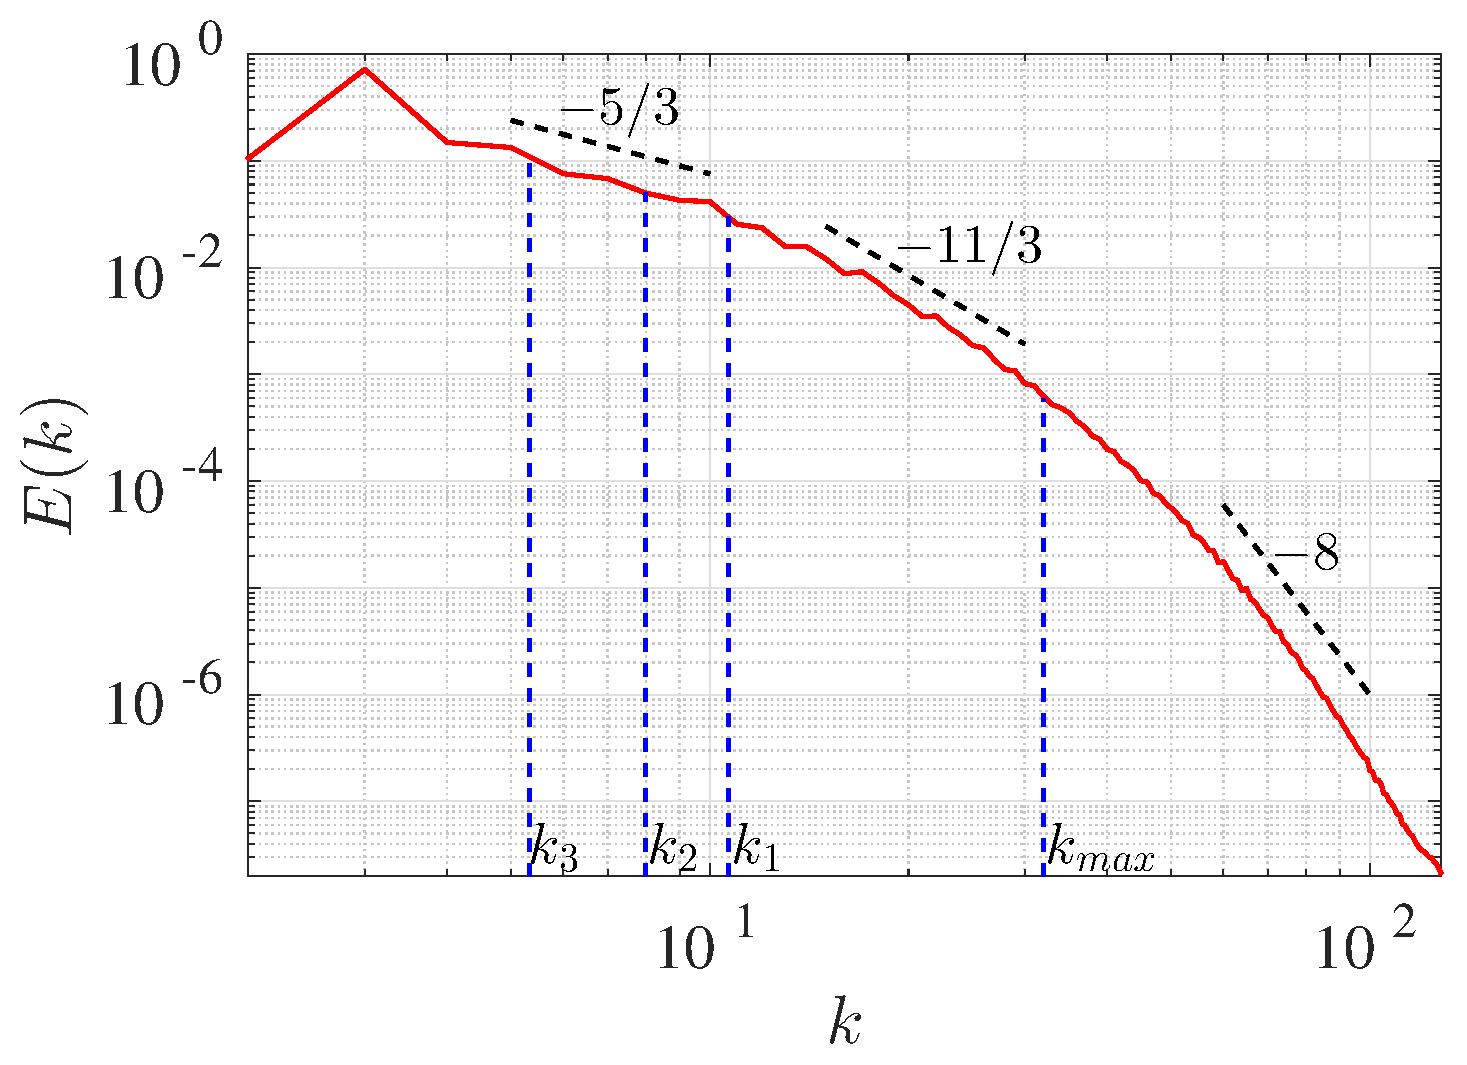
\includegraphics[width=0.65\columnwidth]{./images/datstats/isotropic/spectrum2d_DNS.eps}
	\caption{\label{fig:spectrum2d_DNS} 2D energy spectral of the reference DNS of resolution $ 396^3 $. The maximum real wave number is $ k=128 $ after removing the aliasing contents. Different cutoff wave numbers are shown: $ k_{max} =128/4$ corresponding to the pre-downsampling,  $ k_1 = k_{max}/3 $,  $ k_2 = k_{max}/4 $ and ,  $ k_3 = k_{max}/6 $ for subsampling ratios of $ \sqrt{\dimsh /\dimsl }=3,4 $ and $ 6 $ respectively.}
\end{figure}

Various cases with different ratios are investigated. The subsampling ratios $ \sqrt{\dimsh /\dimsl } $ applied in each direction of space are 3, 4 and 6. These ratios correspond to a number $ \dimsl  $ of HTLS sensors  of $ 32 \times 32 $, $ 24 \times 24 $ and $ 16 \times 16 $ respectively. A sampled HR field with its corresponding subsampled LR field of ratio $ 3 \times 3 $ is shown in figure \ref{fig:u_HR_2D}. Subsampling ratios $ \dimth/\dimtl $ in spanwise direction are 4 , 6 and 8, corresponding to the number of training planes (or key frames) of $ \dimtl =24 $, $ \dimtl =18 $ and $ \dimtl =12 $. Each ratio corresponds to a certain amount of energy loss due to small scales filtered out by an ideal Fourier filter. The energy loss is defined by comparing the filtered fields to the reference ones as in equation \ref{eq:RMS_losses}. The set $ \varmathbb{J}$ now consists of all points thanks to isotropy and homogeneity properties. Table~\ref{tab:energyloss_isotropic} gathers the energy loss due to the 2D or 1D subsamplings.

\section{Concluding remarks}
This chapter has briefly presented the context of the thesis, with the shortage of research tools to measure and compute small scales of turbulence. This problem call for computational methods that permit to estimate such scales from available measurements. We will tackle this problem by seeking: (i) empirical mapping functions between large and small scales, and (ii) fusion models to combine complementary measurements. A wide spectrum of methodologies will be discussed, and their performances will be analyzed using two DNS datasets of either channel flow or isotropic turbulence. Both sets give access to fully resolved fields and permit to design different numerical experiments of various subsampling ratios to obtain virtual measurements. Each configuration is characterized via the kinetic energy loss due to the subsampling. 
\chapter{Velocity reconstruction using regression} 
\label{chap_linearregression} 

This chapter presents regression models to address the problem of estimating high resolution fields from low resolution measurements as defined in section \ref{sec:probdef1}. It reviews the basic ordinary least squares model, regularized linear regression with the common L2 penalty as well as the L1 penalty, and kernel regression. These models are presented in matrix forms, which are more compact than previous works on turbulence. The problem of selecting model complexity and optimizing model parameters, a fundamental topic in learning theory, are also discussed. 

The models are used to reconstruct high-resolution fields from low-resolution measurements. The DNS database of isotropic turbulence presented in section \ref{sec:data_isotropic} are used for illustration. Only partial results on selecting the models and optimizing parameters are shown in this chapter. Optimal models will be used in chapter \ref{chap_comparisons} when comparing performances of all proposed models. 

\section{Regression in turbulence studies}
Regression is probably the earliest method in statistics for prediction. It aims at learning the relation between input variables and corresponding output targets. The model is learned from training samples where both input and output variables are available. the learned model will be used for prediction in situations where only input variables are given. Nice reviews can be found in \citet{bishop2006pattern} and \citet{hastie2009elements}. 

Least squares regression has been applied widely in turbulence studies under the name ``\textit{linear stochastic estimation}'' (LSE) \citep{adrian1977role,adrian1979conditional}. It has been further investigated \citep{guezennec1989stochastic,adrian1992stochastic,ewing1999examination} to estimate conditional eddies from the measurements. Later works introduced various extensions such as multi-time, nonlinear or higher-order LSE \citep{mokhasi2009predictive,durgesh2010multi,nguyen2010proper,meyer2014provide}, which reconstruct velocity fields from pressure or shear-stress measurements. LSE can be also linked to proper orthogonal decomposition (POD), known also as ``principle component analysis'', to reduce the order of reconstruction problems \citep{bonnet1994stochastic}. 

The idea of combining LR velocity measurements to obtain HR fields using regression has not been addressed until recently \citep{melnick2012experimental,tu2013integration}. \citet{melnick2012experimental} used a POD-LSE model to get fully resolved 3D velocities of a flow over a flat plate by combining 3D smoke intensity and 2D PIV measurements. The POD-LSE model has been developed further by \citet{tu2013integration} with a multi-time LSE reconstruction model. Kalman filter or Kalman smoother are used as real time estimation or data post-processing respectively. The model is tested using time-resolved PIV measurements of a bluff-body wake at a low $ Re $.

Regression models in previous works remains rather simple, with the use of POD to reduce the order of the model. However, simple linear regression models suffer from certain limitations. The use of POD, acting as a low-pass filter, neglects certain small scales \textit{a priori}. This work discusses further extensions of simple linear regression based on different regularizations or kernel methods. We aim at maximizing the amount of information that each method can recover, so POD is left aside throughout the thesis. Detailed analysis of reconstruction results such as spectra and errors will assess the performances of regression models as mapping functions between large and small scales. 

\section{Ordinary least squares (OLS)}
Given a set of $ \dimtl $ training samples $ \left\lbrace \left(\y_t, \z_t\right)\right\rbrace, t= 1,2,...,\dimtl $ corresponding to pairs of inputs $ \y_t \in \R^{\dimsl}$ and outputs $ \z_t \in \R^{\dimsh}$, regression models estimate $ \z_t $ as a function of $\y_t $ via a mapping function $ f $: 
\begin{equation}
	f:  \y_t \mapsto  \myhat{\z }_t = f(\y_t) + \n_t
\end{equation}
where $ \n_t \sim \mathscr{N}(0,\sigma^2_{\n_t})$ is usually a white Gaussian noise. $ f $ is learned from the $ \dimtl $ pairs of training samples. This function should minimize the loss $ \loss(f) $, which measures how far the prediction $ f(\y) $ and the reference $ \z $ are different within the training data.

The ordinary least squares model (OLS) assumes that $ f $ is a empirical linear function of $ \y_t $. This model is widely used for its simplicity yet efficiency in situations where only a small training set with low signal-to-noise ratio is given. Assuming that $ \{\z_t\} $ and $ \{\y_t\} $ are mean-free and pre-normalized to one-standard deviation, OLS is expressed as:
\begin{equation}
\myhat{\z }_t = f(\y_t) = \B^{\mytrans}\y_t
\end{equation}
where  $ \B $ is the coefficient matrix of size $ \dimsl \times \dimsh $. The $ i- $th column of $ \B $ tells how to weight each measurement  $ \y_{t,j} $ to get an estimate of $ \z_{t,i} $. The unknown $ \B $ is learned from training data by minimizing the empirical loss:
\begin{equation}
\loss(\B) = \sum^{\dimtl}_{t=1}{ \normtwo{\z_t-\B^{\mytrans}\y_t}	}
\end{equation}
or rearranged in the matrix form as:
\begin{equation}
\loss(\B) = \normtwo{\Y\B-\Z} = \left(\Y\B-\Z\right)^{\mytrans}\left(\Y\B-\Z\right)
\label{eq:LSE2}
\end{equation}
where $ \Y^{\mytrans} \mydef \{\y_t\} $ of size $ \dimsl \times \dimtl $ and $ \Z^{\mytrans} \mydef \{\z_t \} $ of size $\dimsh \times \dimtl$. $ \normtwo{.} $ is the Euclidean distance, also called ``\textit{L2 norm}''. $ \mydef $ is the notation of ``\textit{define as}''. The loss $ \loss(\B) $ is the square of errors, which is purely data-dependent. The optimization problem is to finds $ \B $ such that:
\begin{equation}
\B= \argmin_B{ \left\lbrace \loss(\B) \right\rbrace} = \argmin_B{ \left\lbrace\Vert \Y\B-\Z\Vert^2_2 \right\rbrace}
\end{equation}
$ \argmin{ \{ . \}} $ is the argument of the minimum seeking $ \B $ such that $ \loss(\B) $ attains its minimum. The least square error solution of $ \B $ is by differentiating equation \ref{eq:LSE2} with respect to $\B$ and set to zero:
\begin{equation}
\B= \pinv { \Y } \Z= \left( \Y^{\mytrans}\Y \right)^{-1} \Y^{\mytrans}\Z
\label{eq:LSE5}
\end{equation}
where $ (.)\pinv{} $ is Moore-Penrose pseudo inverse. Then, the output $ \z^\ext  $ of any new input vector $ \y^\ext$ out of the training set is estimated as:
\begin{equation}
\z^\ext = \B^{\mytrans}\y^\ext
\label{eq:LSE6}
\end{equation} 

\section{Regularized linear regression}
\label{sec:regularized_linear_regression}
OLS suffers from critical problems. It requires the inverse of matrix $ \Y^{\mytrans}\Y $ that can be singular or almost singular. The iterative solver can overcome this problem, but may result in a high-variance model with many large coefficients: a small change of $\y^\ext$ leads to very different predictions of $\z^\ext$. Since learned purely from the training data, it often fits very well the training data but poorly performs otherwise. This phenomena is called \textit{overfitting} and will be discussed later in this chapter. Regularized least squares are proposed to overcome this problem. The idea is to add a regularization term $ g(\B) $ on $ \B $ to the data-dependent error term:
\begin{equation}
	\loss(\B, \lambda) = \Vert \Y\B-\Z\Vert^2_2 +\lambda g(\B)
	\label{eq:regularized_linear_regression1}
\end{equation}
where the regularization parameter $ \lambda $ controls the balance between the two terms. Different terms lead to different regression models.

\subsection{Ridge Regression (RR): L2 penalty}
\label{sec:l2_penalty}
The most common and simple regularization is L2 penalty, also called ``weight decay'', which leads to the formulation of ridge regression (RR). The regularization term is on the norm of OLS coefficients, i.e. $ g(\B) = \Vert \B \Vert^2_2$. The loss function becomes:
\begin{equation}
\loss(\B, \lambda) = \Vert \Y\B-\Z\Vert^2_2 +\lambda\Vert \B \Vert^2_2 
\label{eq:RR1}
\end{equation}
The parameter $\lambda $ controls the balance between the data misfit and regularization term, which is the sum of squares of all coefficients. It controls how far $ \B $ are shrunk towards zero, the larger $ \lambda $ the further. Setting the derivative with respect to $ \B $ to zero, the closed form to estimate $ \B $ is:
\begin{equation}
\B=\left( \Y ^{\mytrans}\Y+\lambda \I \right)^{-1}  \Y ^{\mytrans}\Z 
\label{eq:RR2}
\end{equation}
This formula is similar to that of OLS except that some positive value $ \lambda $ is added to the diagonal elements of $ \Y^{\mytrans}\Y $ to ensure $ \Y^{\mytrans}\Y +\lambda \I$ is always invertible.

The mechanism of RR can be analyzed via the singular value decomposition (SVD) of $ \Y $: 
\begin{equation}
\Y= \Umat\Diag\Vmat^{\mytrans}
\label{eq:RR3}
\end{equation}
where $ \Umat=(\mybold{u}_1, \mybold{u}_2,... ,\mybold{u}_{\dimsl}) $ is a $ \dimtl \times \dimsl $ orthogonal matrix, $ \Diag = diag(d_1, d_2, ... , d_{\dimsl} )$ is a $ \dimsl \times \dimsl $ diagonal matrix $ (d_1 \geq d_2 \geq ... \geq d_{\dimsl}) $, and $ \Vmat^{\mytrans}=(\mybold{v}_1^{\mytrans}, \mybold{v}_2^{\mytrans},... ,\mybold{v}_{\dimsl}^{\mytrans}) $ is a $ \dimsl \times \dimsl $ orthogonal matrix. The orthogonality implies that $ \Umat^{\mytrans}\Umat = \I $ or $ \Umat^{\mytrans}=\Umat^{-1} $, similarly for $ \Vmat $ and $ \Vmat^{\mytrans} $. The formula to estimate RR coefficients becomes:
\begin{equation}
\B =\left(\Y^{\mytrans} \Y + \lambda \I\right)^{-1}\Y^{\mytrans}\Z = \Vmat \, diag \left( \frac{d_j^2}{d_j^2+\lambda} \right) \, \Umat^{\mytrans} \Z
\label{eq:RR6}
\end{equation}
Re-estimating training output variables $ \Z $ as a function of inputs, one obtains:
\begin{equation}
\myhat{\Z} = \Y\B = \sum\limits_{j=1}^{\dimsl} \left( \mybold{u}_j \frac{d_j^2}{d_j^2 + \lambda} \mybold{u}^{\mytrans}\right)\Z
\label{eq:RR8}
\end{equation}
This implies that RR projects $ \Z $ onto the principal components of $ \Y^{\mytrans}\Y $ with large energy content (large $ d_j $) and shrinks the coefficients of low energy (small $ d_j $). This makes RR close to the \textit{principal component regression} model discussed in \citet{jolliffe1982note}, where one decomposes $ \Y^{\mytrans}\Y $ using SVD and then set components with low energy content (small $ d_j $) to zeros in a handy manner. The approach also avoids matrix inversion and plays a role similar to regularization.

\subsection{LASSO: L1 penalty}
\label{sec:l1_penalty}
The nature of L2 penalty  is to reduce model variance by shrinking coefficients corresponding to irrelevant events toward zero. However, they are not exactly zero. L1 penalty will precisely force some coefficients to zero. The model is called least absolute selection and shrinkage operator (LASSO) \citep{tibshirani1996regression} in statistics, or basis pursuit denoising (BPDN) \citep{chen1998atomic} in signal processing. It is considered as an implicit subset selection step, where irrelevant events are neglected from the reconstruction. This property favors sparsity - output is estimated as a combination of some input variables only- that is beneficial in many applications.

\begin{algorithm}[t]
\caption{Iterative shrinkage-thresholding algorithm (ISTA)}\label{algo_ISTA}
\begin{algorithmic}[1]
\State Set k=0 and initialize $ \B^{(0)} $; 
\While{not convergence}
	\State $ \bigtriangledown f(\B^{(k)}) = \Y^{\mytrans}(\Z-\Y\B^{(k)})$ \Comment{Residual from step k}
	\State $\B^{(k+1)} \gets \prox_{\lambda \normone{.}} \left[ \B^{(k)} - t^{(k)} \bigtriangledown f(\B^{(k)}) \right] $
	\State k = k + 1 
\EndWhile
\State \textbf{return} $\B^{(k+1)}$
\end{algorithmic}
\end{algorithm}
 
The LASSO cost function is similar to that of RR with a subtle but very important modification:
\begin{equation}
F(\B)= \Vert \Y\B-\Z\Vert^2_2 +\lambda \normone{\B}
\label{eq: LASSO1}
\end{equation}
The data-dependent term is the same as OLS or RR. The different penalty term $ \lambda \normone{\B}$ imposes a constraint on the sum of absolute values of coefficients. This modification leads to sparsity, the key difference between LASSO and RR. It also makes the problem nonlinear and there exits no closed-form solution. Gradient-based methods are usually used to solve this optimization problem. Iterative shrinkage-thresholding algorithms (ISTA) is one of them, where $ \B $ is solved iteratively by \textit{soft-thresholding} as in Algorithm \ref{algo_ISTA} \citep{daubechies2004iterative}. In the pseudo code, $ prox $- the shrinkage operator- is the element-wise soft-thresholding: 
\begin{equation}
\left(\prox_{\lambda \normone{.}}[\B]\right)_i =
\begin{cases}
b_i-\lambda \mysign{b_i} & \text{if } |b_i|>\lambda,
\\
0 & \text{otherwise }
\end{cases}
\end{equation}
where $ t^{(k)} $ is the gradient step size, $ b_i $ is the $ i- $th coefficient of $ \B $. The \textit{sign function} $ \mysign{b_i} $ is defined as:
\begin{equation}
 \mysign{b_i} =
\begin{cases}
-1 & \text{if } b_i<0,
\\
0 & \text{if } b_i=0,
\\
1  & \text{if } b_i>0.
\end{cases}
\end{equation}
Faster schemes have been proposed to accelerate the convergence time \citep{vonesch2008fast,beck2009fast}, but further discussions are outside the scope of this work.

LASSO often outperforms RR and subset selection methods for several reasons. Compared to RR, LASSO takes most of the advantages, including the stability of the solution and the shrinkage feature. These features give a low-variance model compared to subset selection method. Moreover, LASSO favors sparsity, which can be considered as an implicit subset selection \citep{hastie2005elements, hastie2009unsupervised}. By forcing some of the coefficients to zeros, the irrelevant predictors are suppressed in final estimation.

\section{Nonlinear regression}
\label{sec:nonlinear_regression}
Linear regression aims at mapping the output as a linear combination of input variables. This implies a real constraint on performances of this family of models. In many cases including turbulence, linear functions are too simple to describe the undergoing phenomenon. Nonlinear regression models are beneficial, and kernel feature mapping is often used.

\subsection{Feature mapping}
Kernel methods are used to introduce nonlinearity into the model. The idea is to project the original input vector $ \y  $ onto a fixed feature space:
\begin{equation}
\y_t \mymapto \mybold{\phi}_t = \featmap{\y_t}
\end{equation}
and perform least square regression in this space. $ \y_t \in \R^{\dimsl}$ is the $ t- $ input vector. The feature vector $ \mybold{\phi}_t \in \R^{\Df} $, where $ \Df \gg \dimsl $ is the dimension in feature space. The least square problem becomes: 
\begin{equation}
\B = \argmin_B{ \left\lbrace \normtwo{ \Z- \mathbf{\Phi}\B} \right\rbrace}
\end{equation}
where $ \mathbf{\Phi} = \{\mybold{\phi}_t \} $ ($ t = 1, ..., \dimtl $), the so-called \textit{design matrix}, is of size $ \dimtl \times \Df $. Adding L2 regularization term $ \normtwo{\B} $ and deriving analogously as RR model, the solution is:
\begin{equation}
\B=\left(\mathbf{\Phi}^{\mytrans}\mathbf{\Phi} + \lambda \I\right)^{-1}\mathbf{\Phi}^{\mytrans}\Z
\end{equation}
Then the prediction of a new input variable $ \y^\ext $ is:
\begin{equation}
\z^\ext=\B^{\mytrans} \featmap{\y^\ext}
\end{equation} 

\subsection{Kernel ridge regression}
Involving nonlinearity via feature mapping significantly increases computational costs. The kernel trick is proposed \citep{saunders1998ridge} to overcome this problem, resulting in the so-called kernel ridge regression (KRR) model. This trick appears when solving ridge regression using Lagrange dual optimization.

\subsubsection*{Dual form of ridge regression}
RR in equation \ref{eq:RR1} can be re-expressed as a dual Lagrangian optimization problem:
\begin{equation}
\B=\argmin_B{ \left\lbrace \sum\limits_{t=1}^{\dimtl}\normtwo{\mybold{e}_t} + \lambda \normtwo{\B} \right\rbrace } \subjectto \z_t - \B^{\mytrans}\y_t = \mybold{e}_t, \:\:\:\:\:\: t = 1, 2, ..., \dimtl
\label{eq:RRdual1}
\end{equation}
where $ s.t $ stands for ``\textit{subject to}''. Introducing Lagrange multipliers $ A[\dimtl \times \dimsh] \mydef \{\mybold{a}_t^{\mytrans} \} (t = 1, 2, ..., \dimtl), \mybold{a}_t \in \R^{\dimsh}$, the optimization problem \ref{eq:RRdual1} is equivalent to the problem of finding the saddle point of the function:
\begin{equation}
\sum\limits_{t=1}^{\dimtl}\normtwo{\mybold{e}_t} + \lambda \normtwo{\B} + \sum\limits_{t=1}^{\dimtl} \mybold{a}_t^{\mytrans}\left( \z_t - \B^{\mytrans}\y_t - \mybold{e}_t\right)
\end{equation}
The solution as shown in \citet{saunders1998ridge} is:
\begin{equation}
\mathbf{A}  = \left(\mathbf{K} + \lambda \I\right)^{-1}\Z
\end{equation}
where $ \mathbf{K} \mydef \Y\Y^{\mytrans} $ is the matrix of dot products, $ \mathbf{K}_{m,n} = \y _m^{\mytrans} \y _n $. The prediction for a new input variables $ \y^\ext $ is:
\begin{equation}
\myhat{\z }^\ext = \left(\sum\limits_{t=1}^{\dimtl}\mybold{a}_t^{\mytrans}\y_t\right)\y^\ext = \mathbf{A}^{\mytrans} \mybold{k}^{\ext}
\end{equation}
where $ \mybold{k}^{\ext} \mydef \{k_t\} = \{ \y_t^{\mytrans} \y^\ext \} \in \R^{\dimtl}$.
 
\subsubsection*{Kernel trick}

\begin{table}
\centering
\begin{tabular}{lc} \toprule
	Function name  & $ k (\mybold{u}, \mybold{v}) $ \\ \midrule
	Linear  & $ \mybold{u}^{\mytrans} \mybold{v} $ \\ \midrule
	Polynomial  & $ (r + \mybold{u}^{\mytrans} \mybold{v})^d $ for $ r,d \geq 0 $\\ \midrule
	Radial basis function (RBF)  & $ \myexp{-\gamma \normtwo{\mybold{u} - \mybold{v}}}$, $ \gamma > 0 $ \\
	\bottomrule
\end{tabular}
\caption{Common basis functions for kernel methods.}
\label{tab_basisfunctions}
\end{table}

Solving RR in the dual form offers no improvement of accuracy, speed or stability. However, the beauty of this approach is the presence of only dot products among input variables in the final prediction step. This implies an analogous procedure when working in a nonlinear feature space. The transformation into such a space is unnecessary if the dot products of the transformed variables can be estimated using the kernel: 
\begin{equation}
k (\mybold{u}, \mybold{v}) = \featmap{\mybold{u}}^{\mytrans} \featmap{\mybold{v}}
\end{equation}
This explicit transformation is computed in time $ \mathcal{O}(\dimsl^2) $, where $ \dimsl $ is the dimension of the input vectors. The \textit{kernel trick} permits to estimate directly $ k (\mybold{u}, \mybold{v}) $ without computing $ \featmap{\mybold{u}} $ and $ \featmap{\mybold{v}} $, reducing the computational time into $ \mathcal{O}(\dimsl) $ only. Not every kernel has this property. Table \ref{tab_basisfunctions} gathers three common functions.

\section{A framework to select model and parameters}
A model is assessed via its generalization performance, i.e. the prediction capability on a new dataset independent from the training set. In all above models, there exists one or more hyper-parameters that are directly linked to model performances. The arising question is how to optimize those parameters using training data only in a systematic manner. This step is the so-called \textit{parameter optimization}, while the step to test performances of the model on independent data is the so-called \textit{model assessment}. 

It is worth also mentioning the definition of different datasets: \textit{training}, \textit{validation} and \textit{test} sets. The training set contains data from which a model is learned. The validation set is used to estimate prediction errors, and from which the best model is chosen. This model is the one that gives the most accurate prediction on the validation set. The testing set is finally used to give an estimate of the prediction error of this optimal model. This error is approximately the generalization error on independent datasets.

To optimize the generalization capability of a model, one needs to understand the idea of \textit{bias} and \textit{variance}. Next sections will discuss this topic, with the technique called ``\textit{cross-validation}'' to find the trade-off between bias and variance using the training data only. 

\subsection{Bias-variance trade-off}
The above regression models can be interpreted as seeking a mapping function $ f $: 
\begin{equation}
	f:  \y  \mapsto  \myhat{\z } = f(\y ) + \n
\end{equation}
where $ \n \sim \mathscr{N}(0,\sigma^2_{\n})$ is assumed to be a white Gaussian noise. The expected prediction error of this model for an input vector $ \y_\knot $ is:
\begin{equation}
\begin{split}
\epsilon(\y_\knot) & =\E{\left(\z_\knot - f(\y_\knot)\right)^2} \\
  & = \underbrace{\sigma_{\n}^2}_{\text{Irreducible Error}} + \underbrace{\left(\E{\myhat{\z }_\knot} - \z_\knot\right)^2}_{\text{Bias}^2} + \underbrace{\E{\left( \myhat{\z }_\knot -  \E{\myhat{\z }_\knot} \right)^2}}_{Variance}
\end{split}
\end{equation}
where $ \E{.} $ is the expectation of a variable. The first term comes from the noise, which depends only on the data and is irreducible. The second term is the square bias, showing how far the average of the estimates is different from the true mean. The last term is the expected variance of the estimate around its mean. We can interpret the bias as the average prediction error over different data sets from the true mean, and the variance as how this error is sensitive to a particular choice of data set.

After the decomposition, a model is said to be \textit{underfitting} or \textit{overfitting} depending on the contribution of each term in the total error. An underfitting model is too simple to capture all details of the underlying phenomenon. This model is high-bias and low-variance: it poorly fits the training data and performs similarly in the testing data. An overfitting model is over-complex: it closely fits the training data, including noises, and gives poor performance on new testing data. This model has low bias and high variance. Ideal models should have both low bias and variance. In practice, a good model must satisfy its \textit{bias-variance trade-off} when it does not suffer from either the problems of overfitting or underfitting.  

\begin{figure}
\centering
	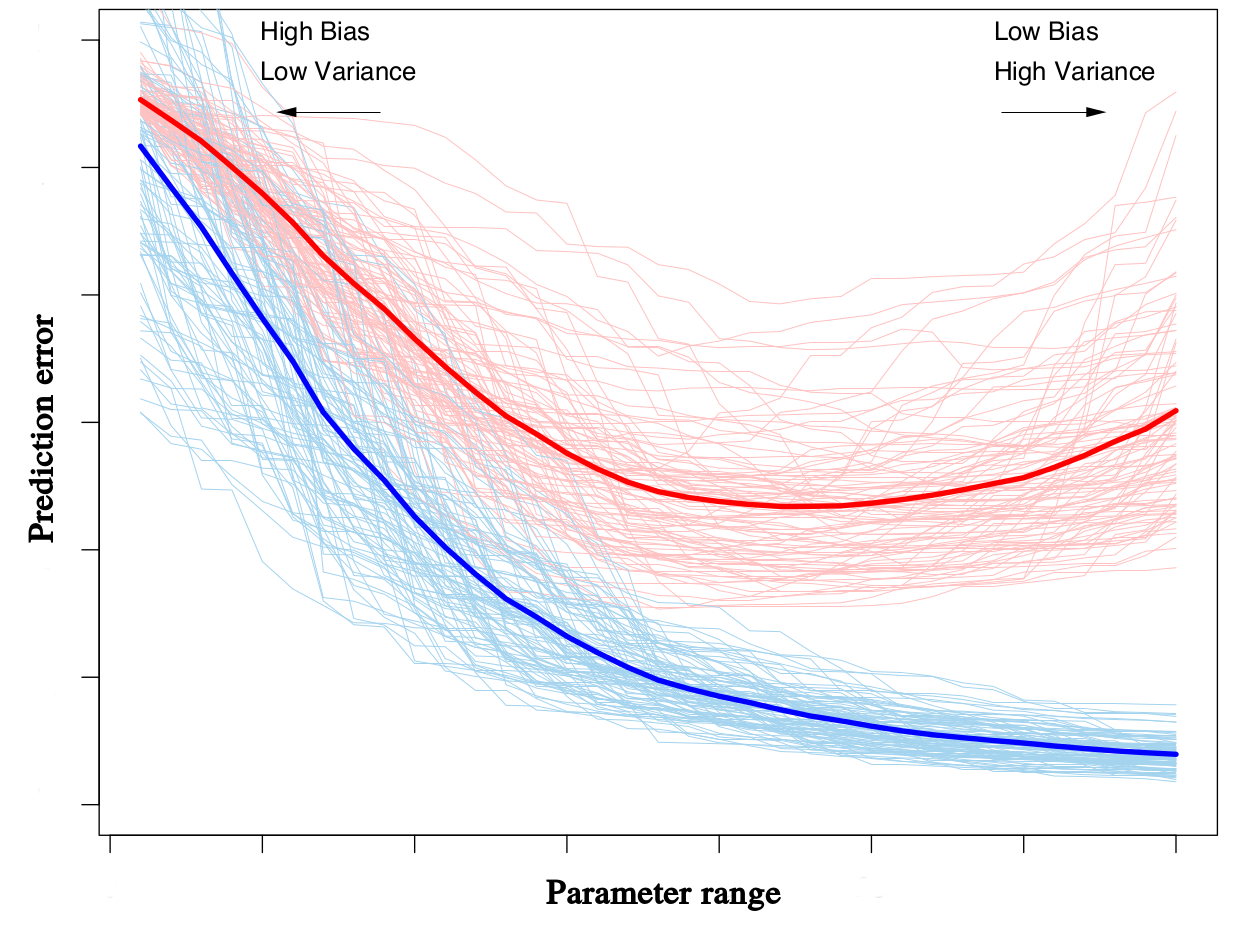
\includegraphics[width=0.7\columnwidth]{./images/regression/bias-variance_tradeoff.png}
	\caption{\label{fig:bias-variance_tradeoff} Typical behavior of prediction error for testing (red) and training (blue) dataset as a function of a hyper-parameter \citep{hastie2009elements}. Different curves are for various datasets. The solid ones are expected errors (average of all curves). From left to right can be the direction of decreasing regularization or increasing model complexity.}
\end{figure}

The idea of underfitting and overfitting can be visualized in figure \ref{fig:bias-variance_tradeoff} as modified from \citet{hastie2009elements}. It shows the prediction errors for training and testing datasets as a function of a parameter. This parameter can be either the model complexity in an increasing order or the regularization parameter $ \lambda $ in a decreasing order. Models toward the left (low complexity model, or regression with a strong regularization) are underfitting. It does not fit well both the training and testing data. Toward the right, errors on the training set decrease, while those of the testing set decrease and then increase again. Models in the far right are overfitting. They fit well the training set but not the testing set. The desired model is the one such that the error on the testing set is the lowest. At this point, the model reaches its bias-variance trade-off: bias and variance do not necessarily reach their minima, but a compromise ensures the minimal error on testing data.

The idea of bias-variance trade-off can be further visualized schematically as in figure \ref{fig:bias-variance} \citep{hastie2009elements}. The blue-shaded region shows the irreducible error $ \sigma_{\n}^2 $ (due to random noise) of the training set, where the truth is at the center and all realizations are within. To fit the model, the non-regularized model space (red curve) contains all possible models, while the magenta one shows the restricted space of regularized models. Model variances are depicted as yellow curves centered at the so-called ``closest fit''. The model bias is the distance of the closest fit and the truth, which can only be reduced as increasing the model complexity or adding more features. Regularized models add estimation bias on top of the model bias but reduce the variance. The benefit of the trade-off is only when the variance is reduced more than the squared estimation bias.

\begin{figure}
\centering
	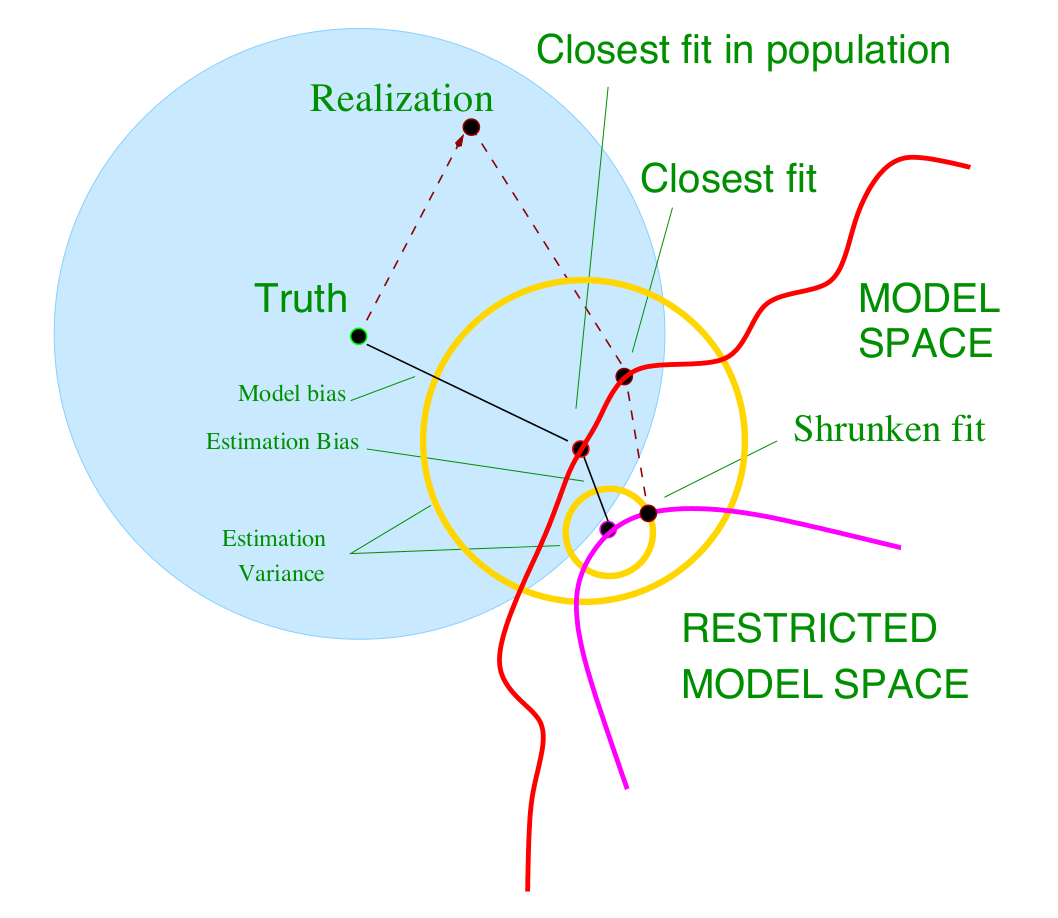
\includegraphics[width=0.6\columnwidth]{./images/regression/bias-variance.png}
	\caption{\label{fig:bias-variance} Schematic view of the behavior of bias and variance \citep{hastie2009elements}. The blue-shaded, centered at the truth, is the realization space, where maximum distance is the irreducible error. All possible models are bounded by the red/magenta model space curves. Bias is shown by the black lines as the distance to the truth. Best models are shown as black dots, and circled by model variances. }
\end{figure}

The bias-variance trade-off is essentially estimated from the training data. If this set is large enough, it can be virtually divided into training, cross-validation and testing sets. A general advice for the size of these three sets is $ 50 \% $, $ 25 \% $ and $ 25 \% $ respectively \citep{hastie2009elements}. However, learned models are usually improved when using more data. Cross-validation is another idea to find the trade-off while keeping the whole training data for learning the model. 

\subsection{Cross-validation}
In many cases, the training data is limited. Setting aside $ 50 \% $ the data to quantify the model might lose all the benefits from regularization and nonlinearity compared to OLS. Cross validation (CV) is commonly used to select the model and optimize parameters using all given data. 

The most popular CV technique is \textit{k-fold} CV. The dataset is randomly split into $ K $ subsets of approximately equal size. For each $ K $-th subset to estimate the prediction error, the model is trained on the remaining $ K-1 $ subsets. This procedure is repeated $ K $ times for all the subset, and the model error for the current setting is the average of its $ K $ estimates. A summary of k-fold CV is presented in algorithm \ref{algo_kfold}. $ K $ is at most the number of training samples (\textit{leave one out cross validation}). When $ K $ is high, the selected model tends to have lower bias but higher variance, since many training samples are similar. A much heavier computation is also required, since the training/predicting is repeated $ K $ times. The popular choice of $ K $ is from 5 to 10 \citep{breiman1992submodel, kohavi1995study}. 

\begin{algorithm}[t]
\caption{K-fold cross-validation for set of L parameters $ \gamma_1, \gamma_2, ..., \gamma_L $} \label{algo_kfold}
\begin{algorithmic}[1]
	\State Divide the training samples into k folds randomly
	\For {$ i = 1, 2, ..., L$}
		\For {$ j = 1,2,... K $}
			\State Train the model with $ \gamma_i $ using all data set except the $ j^{th} $
			\State Estimate prediction error $ \epsilon(i,j) $ of the model on the $ j^{th} $ set
		\EndFor
	\EndFor
	\State Estimate averaged error $ \epsilon(i) = \frac{1}{K}\sum\limits_{j=1}^{K}\epsilon(i,j)$
	\State Return optimal parameter $ \gamma_m $ where $ \epsilon(m) = min \{\epsilon(i)\}$.
\end{algorithmic}
\end{algorithm}

\section{Regression models for reconstruction of isotropic turbulence}
We now apply regression models to reconstruct HR velocity fields from LR measurements. The data from DNS isotropic turbulence discussed in section \ref{sec:data_isotropic} is used. Streamwise velocities from $ 37 $ data cubes of fully resolved data $ 96^3 $ are used as the reference. In each data cube, only the streamwise velocity component is considered. The training examples are the HR fields (in spanwise-vertical directions) and equivalent LR ones subsampled by a factor of $ \sqrt{\dimsh/\dimsl} = 3 $ in both vertical and spanwise directions. This ratio is equivalent to an energy loss of $ \Delta \kappa_s = 1.03 \% $ (see table \ref{tab:energyloss_isotropic}). In streamwise direction, the training planes are selected every 4 snapshots, corresponding to an energy loss of $ 1.23 \% $. This configuration is chosen to mimic other problems investigated later in chapters \ref{chap_NLM} and \ref{chap_BayesianFusion}. 

Regression models are learned from $ 37 \times 24 $ pairs of LR ($ \dimsl = 32 \times 32 $) and corresponding HR ($\dimsh = 96 \times 96 $) fields. The learned models are then used to reconstruct all $ 37 \times 96 $ HR fields from $ 37 \times 96 $ measured LR planes. These results are presented latter in chapter \ref{chap_comparisons} when comparing various methods. Following sections only discuss the optimization of model parameters.

\subsection{Regularization parameter and shrinkage effect}
Ordinary least squares model inverses directly $ \Y^{\mytrans}\Y $, which is usually ill-conditioned, leading to high variance models. A slight change of input variables can lead to very different predictions. Regularization is introduced to reduce this effect by imposing different penalty terms on regression coefficients. RR seeks a model with small sum-of-square coefficients, LASSO imposes a penalty of their absolute values (see section \ref{sec:regularized_linear_regression}). 

\begin{figure}
\centering
	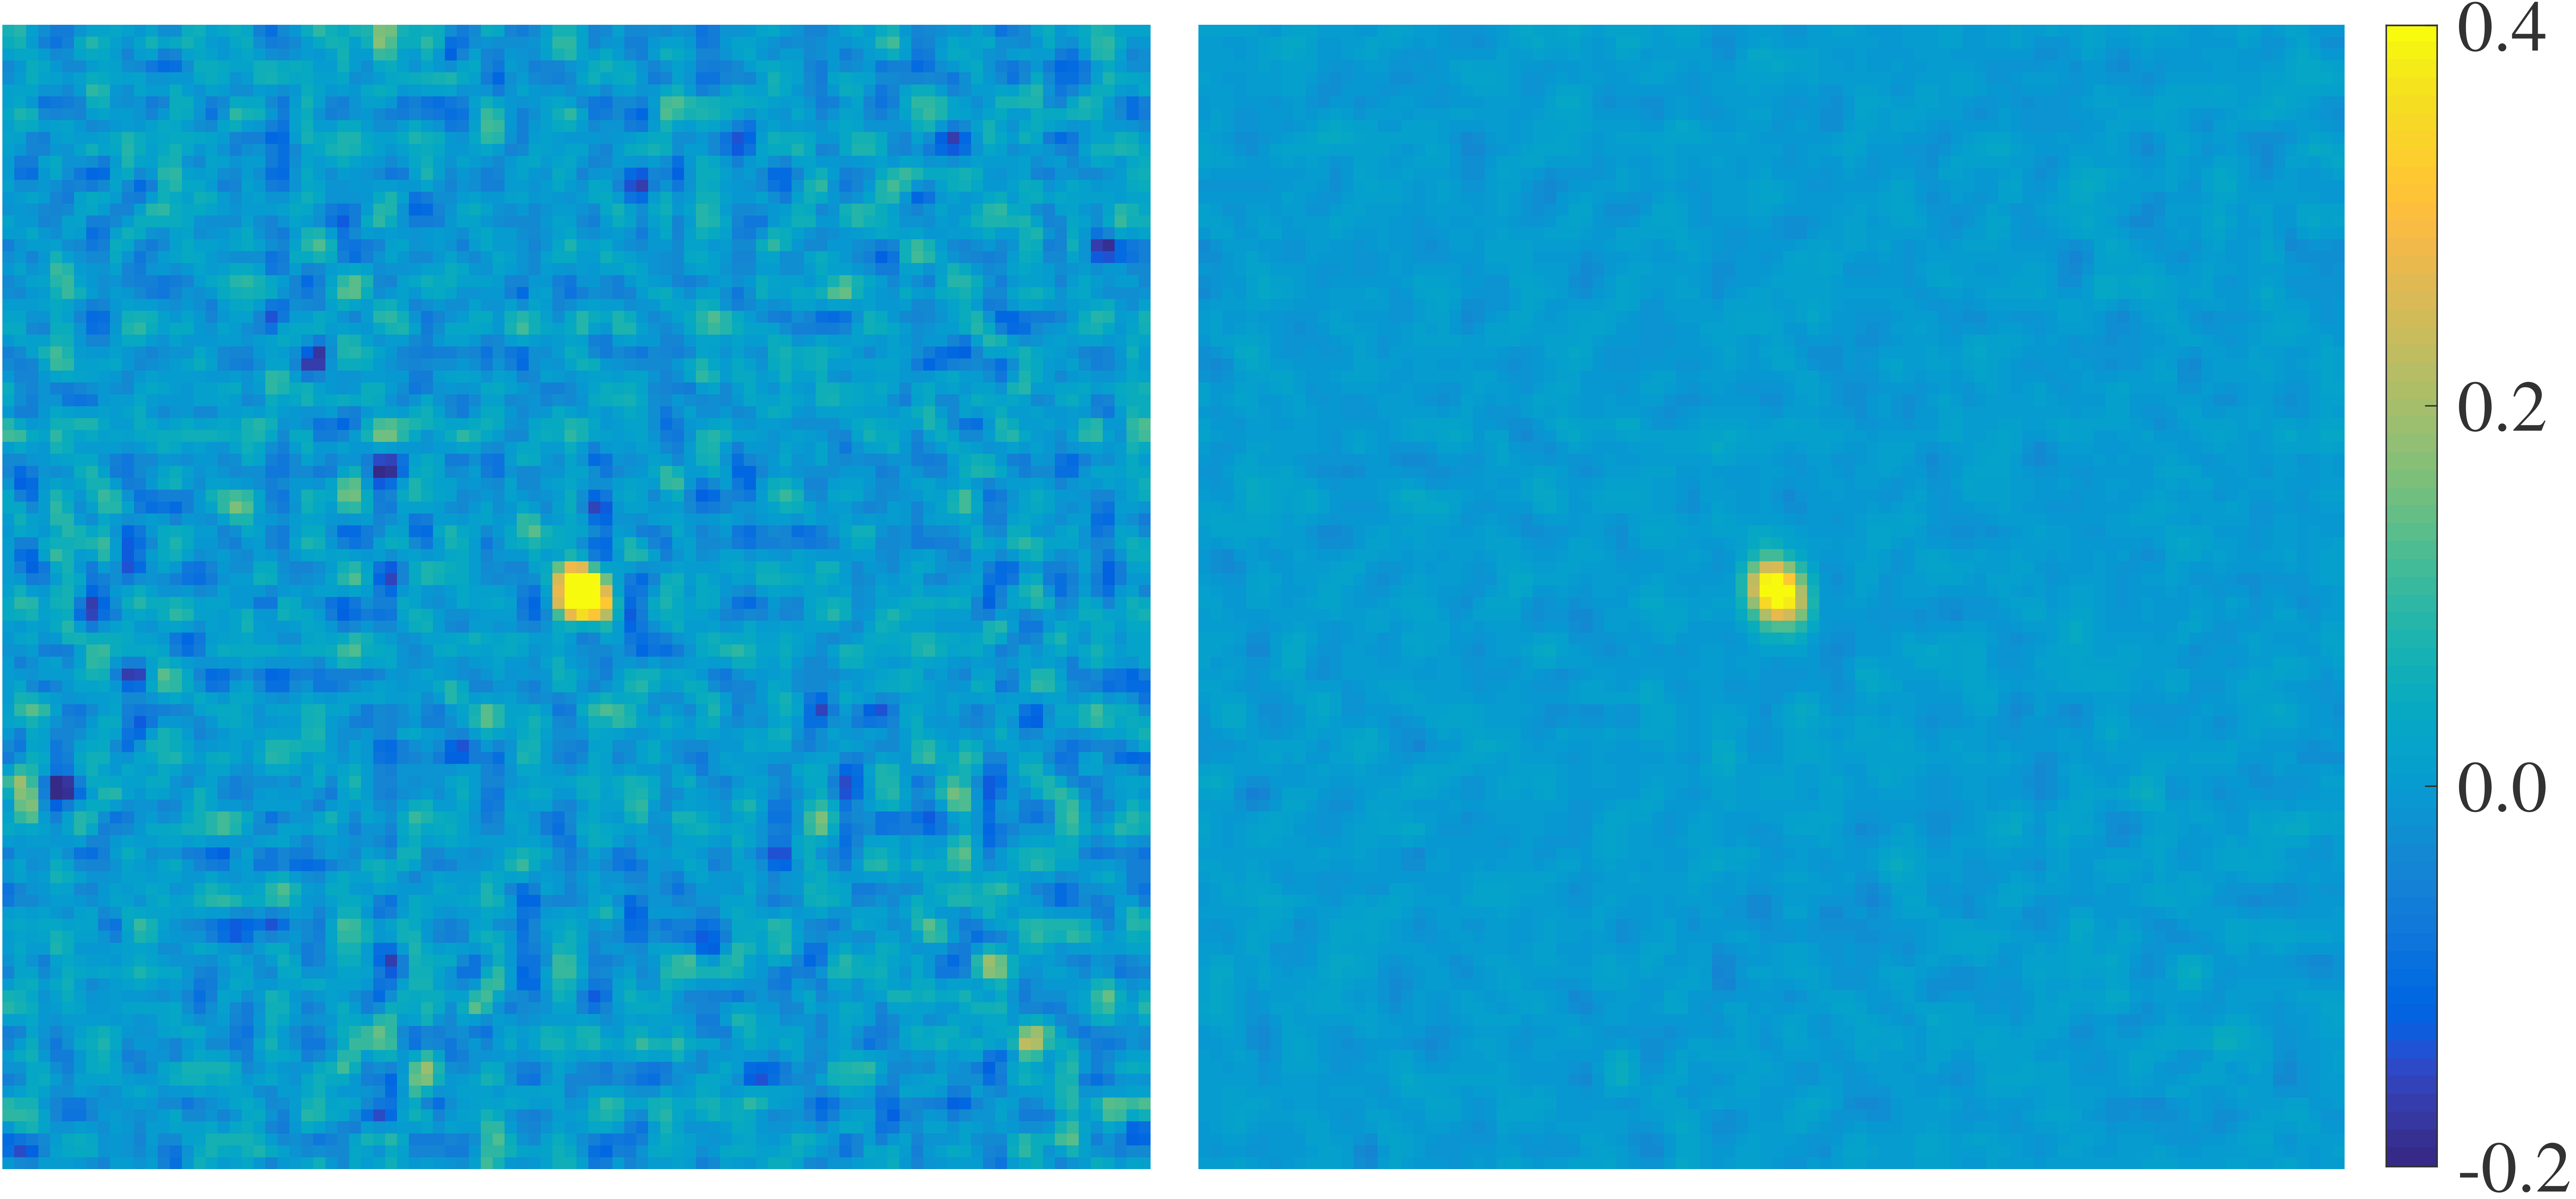
\includegraphics[width=0.8\columnwidth]{./images/regression/RR_LSE_coefficients.png}
	\caption{\label{fig:RR_LSE_coefficients} Shrinkage effect: coefficients of OLS (left) vs RR (right) models correspond to an input LR measurement at the center of the field. The coefficients, which are rearranged in a 2D field of the size $ 96 \times 96 $, can be interpreted as the contributions of this input to the reconstruction of all other high-resolution points. The higher the coefficient, the stronger the impact.}
\end{figure}

Figure \ref{fig:RR_LSE_coefficients} shows the weight of the input variable at the center of the field in reconstructing all other HR points by OLS and RR. These are the coefficients $ \mybold{b}_j \mydef [b_{j1}, b_{j2}, ..., b_{j\dimsh}]^{\mytrans}$ computed in equation \ref{eq:LSE5} for OLS or equation \ref{eq:RR2} for RR. Recall that $ \B $ is of size $ \dimsl \times \dimsh $. The figures are $ \mybold{b}_j$ of OLS and RR models, where index $ j $ corresponds to the central point. $ \mybold{b}_j $ is then rearranged to recover the 2D shape of size $ \sqrt{\dimsh} \times \sqrt{\dimsh} $ of the 2D velocity fields. In both plots, the weights remain significant in a neighborhood of several pixels. The coefficients drop very quickly when moving away from the center. This is due to the rapid decay of correlation between the central point and its neighbors. The difference between the two methods is that OLS (using direct inversion) gives large coefficients almost everywhere whereas RR shrinks the contributions of irrelevant points to small values.

\begin{figure}[t]
\centering
	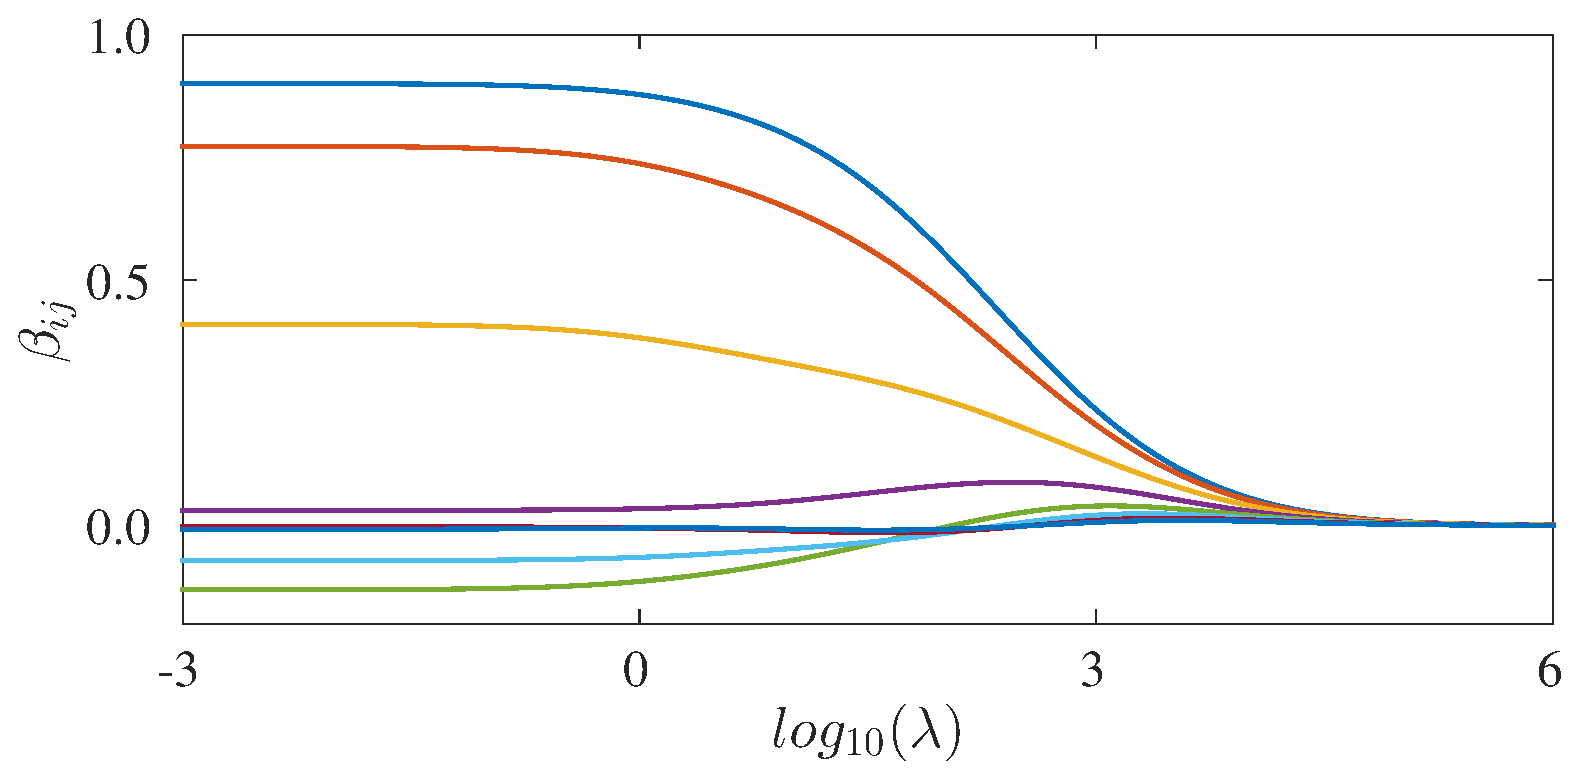
\includegraphics[width=0.8\columnwidth]{./images/regression/RR_coeffs_lambda.eps}
	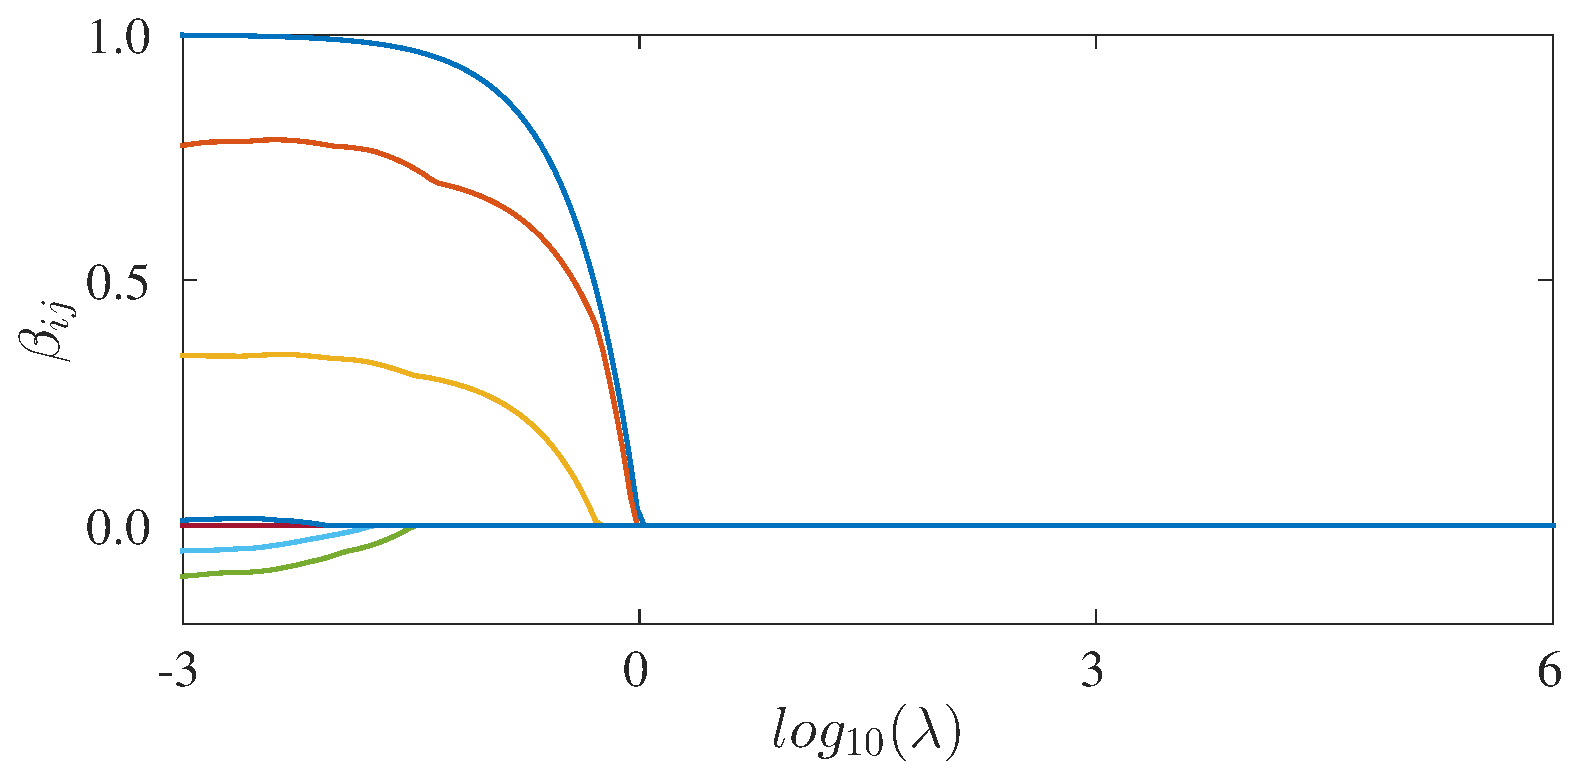
\includegraphics[width=0.8\columnwidth]{./images/regression/Lasso_coeffs_lambda.eps}
	\caption{\label{fig:coeffs_lambda} Shrinkage effects of L2 (top) and L1 (bottom) penalty: coefficients corresponding to eight high-resolution outputs (in eight different colors) as functions of regularization parameters $ \lambda $. Higher $ \lambda $ shrink the coefficients toward zeros differently depending on the penalty terms.}
\end{figure}

The different shrinkage behaviors of RR and LASSO are visualized in figure \ref{fig:coeffs_lambda}. This figure shows the eight different coefficients corresponding to eight HR outputs as a function of the regularization parameter presented in equation \ref{eq:regularized_linear_regression1}. It confirms the effect of the penalty term, which shrinks coefficients associated with irrelevant inputs to zeros. RR coefficients do not reach exact zeros even for extremely high $ \lambda $, while LASSO rapidly shrinks some coefficients to exact zeros.

\subsection{Optimizing regularization parameters and model complexity via ten-fold cross-validation}	

All regression models (except OLS) are parametric, i.e. at least one hyper-parameter controls the construction of the model and its performances. With RR, LASSO or KRR, the regularization parameter $ \lambda $ controls the balance between data misfit and regularization term. KRR model is also a function of the kernel parameter, which is the standard deviation of the distribution when using RBF kernel, or the polynomial order. All hyper-parameters are chosen from the training samples using ten-fold CV (see algorithm \ref{algo_kfold}). The plot of the error as a function of model parameters is called the ``validation curve'', from which the best model or parameter is selected.

Another important test is to see whether the training dataset is sufficient or not. This is examined via the so-called ``learning curve''. To estimate this curve, a small subset of data is drawn out randomly from the training set. This set is retained to estimate the error at the last step. For the remaining data, models are optimized using different portions. Trained models are assessed by computing prediction errors on the testing data. The curve of errors as a function of different data size, the ``learning curve'', will tell whether the current training data is sufficiently large to guarantee an accurate learning.

\begin{figure}
\centering
	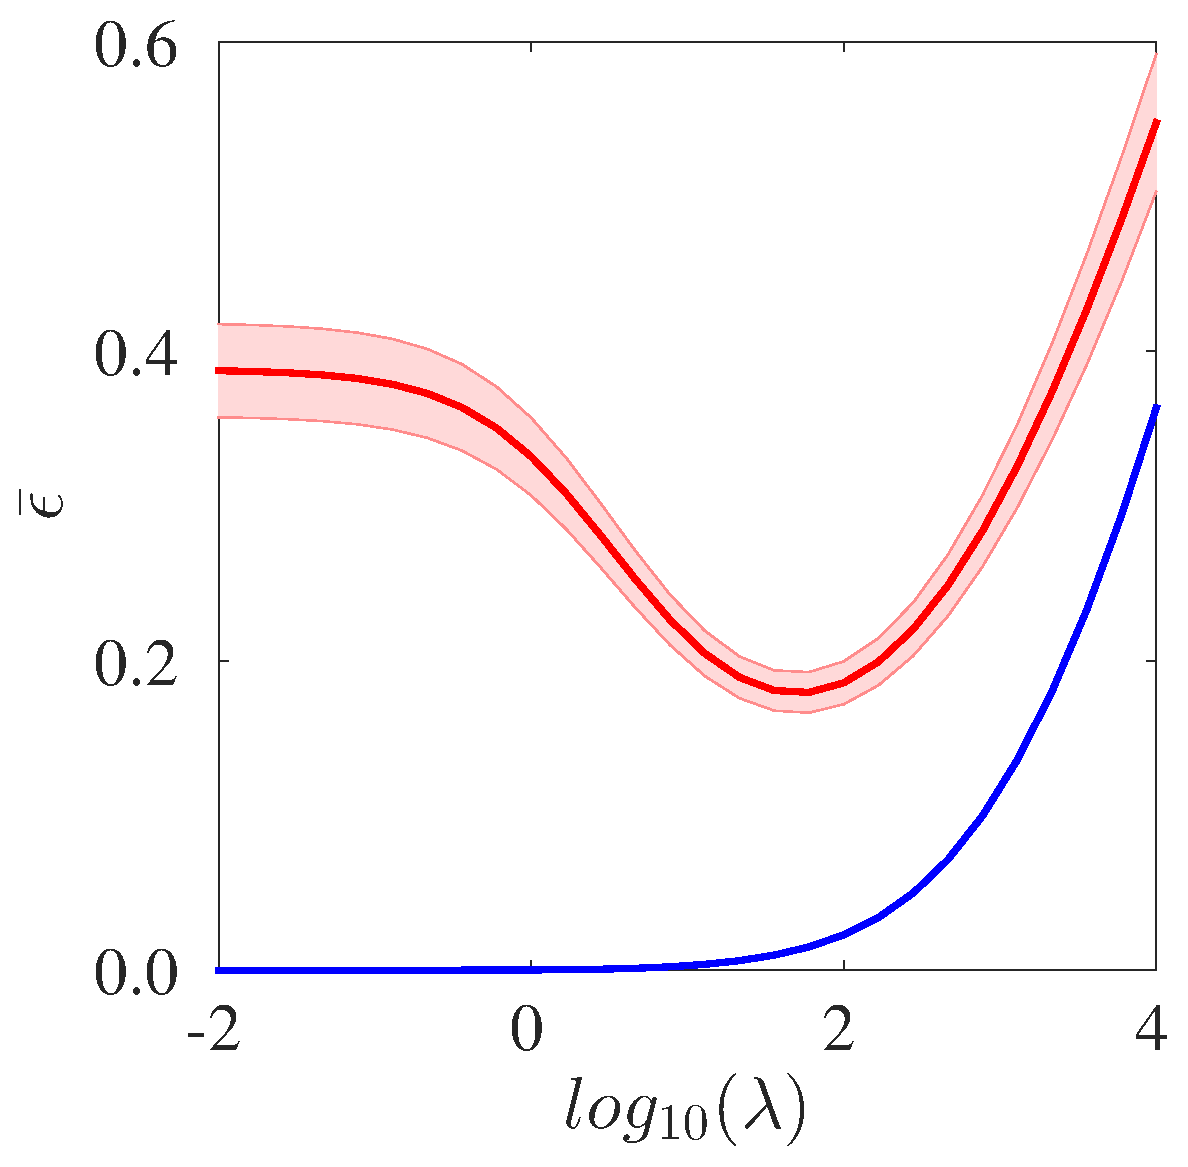
\includegraphics[height=6.75cm]{./images/regression/RR_validationcurve.eps}
	\hspace{0.3cm}
	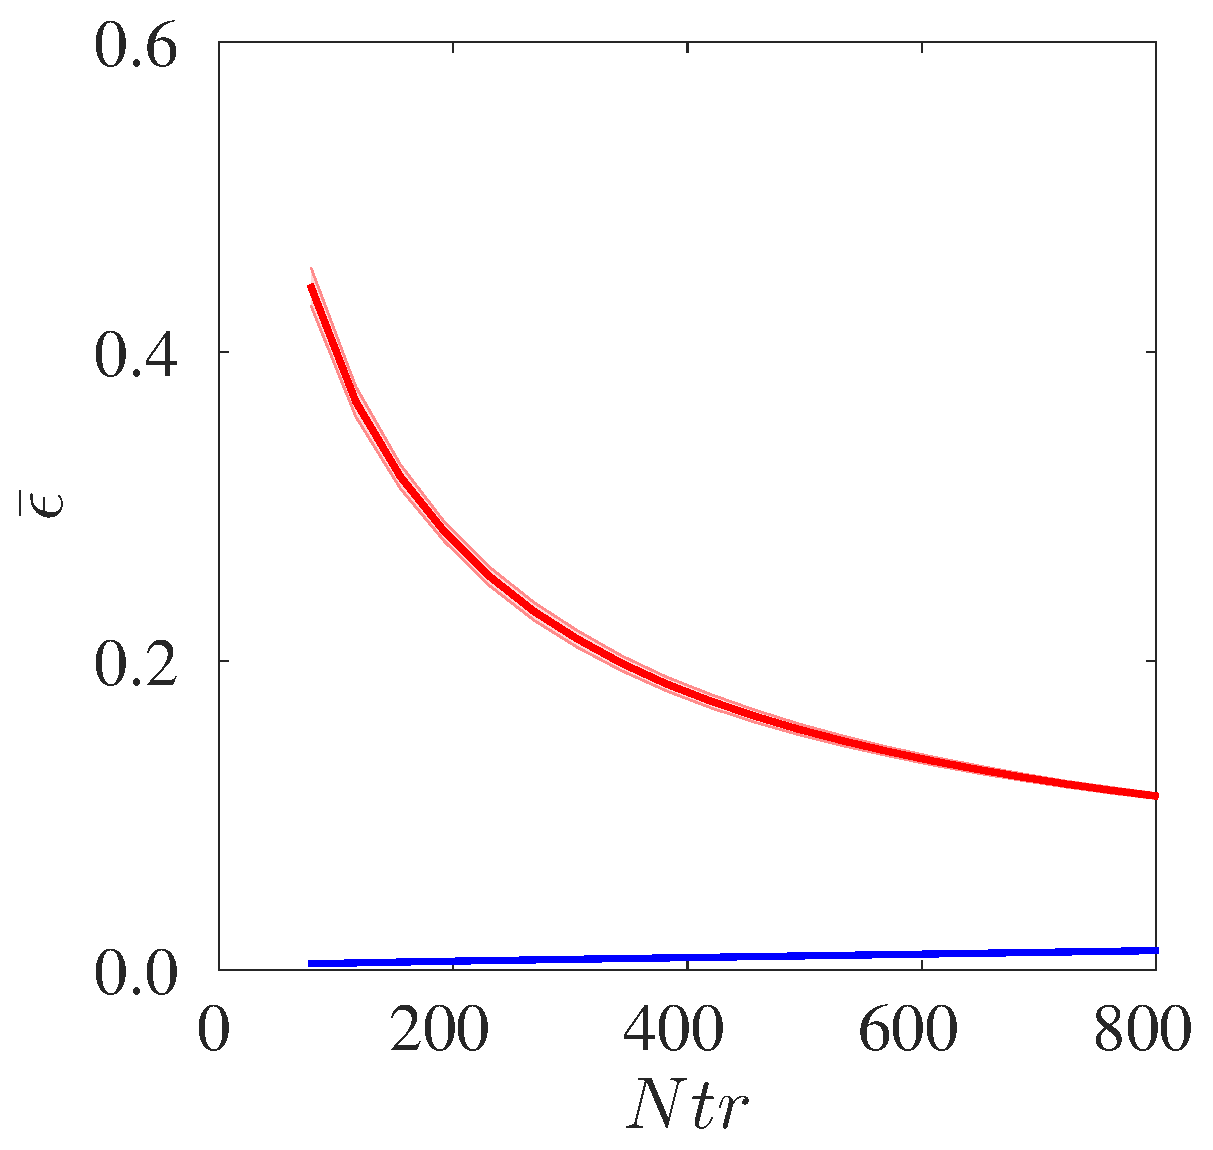
\includegraphics[height=6.75cm]{./images/regression/RR_learningcurve.eps}	
	\caption{\label{fig:RR_validationcurve} RR validation curve: errors as functions of regularization parameter $ \lambda $ (left), and learning curve: errors as functions of training data size (right). Red curves are for the prediction, while blue ones are for the training data}
\end{figure}
\begin{figure}
	\centering
	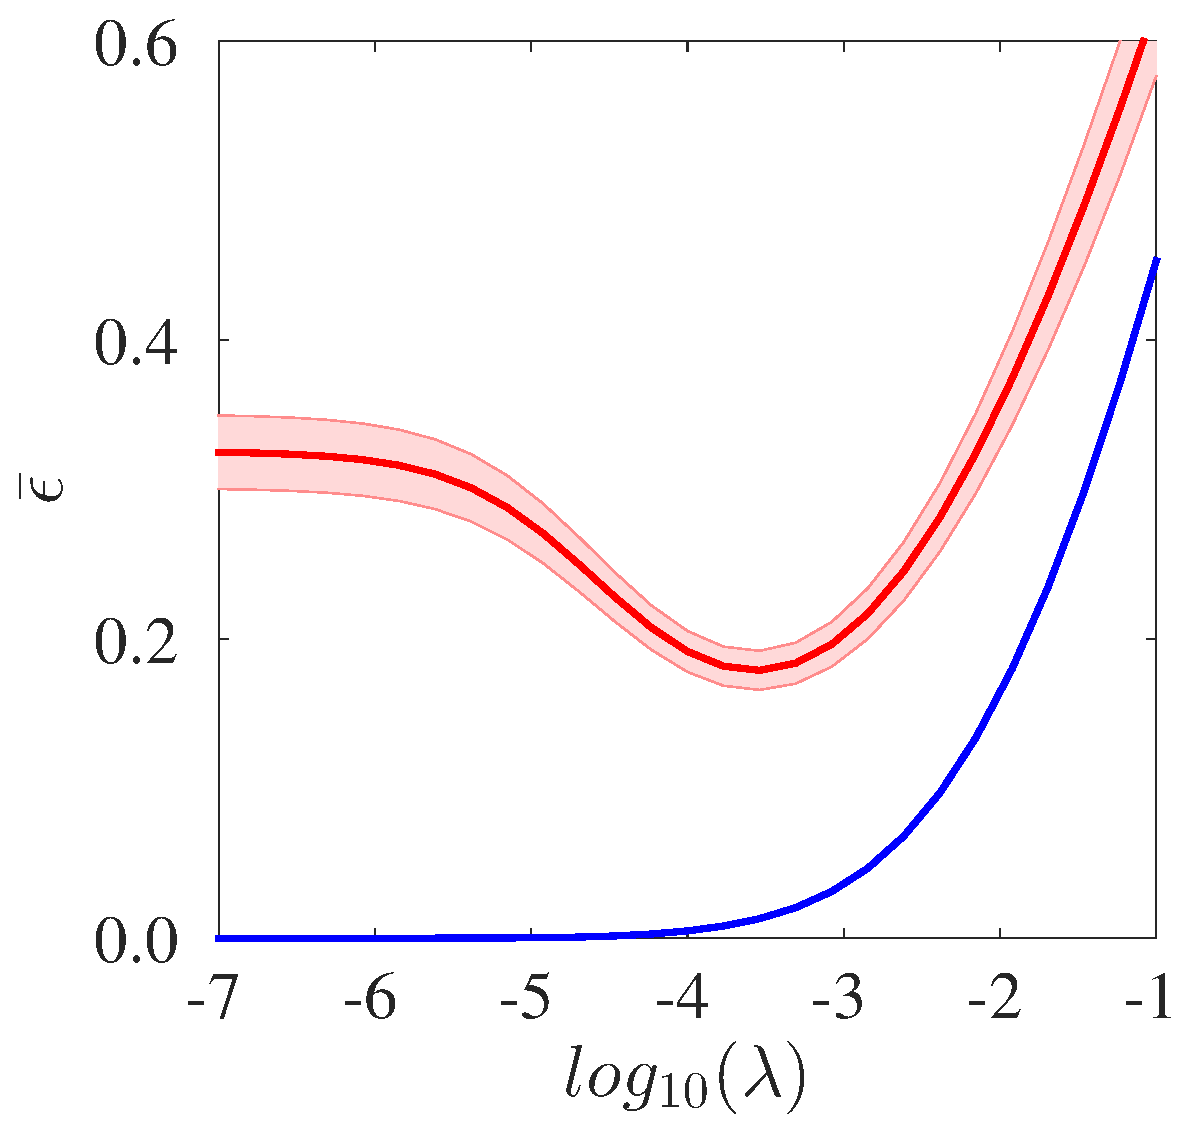
\includegraphics[height=6.75cm]{./images/regression/KRR_validationcurve_lambda.eps}
	\hspace{0.3cm}
	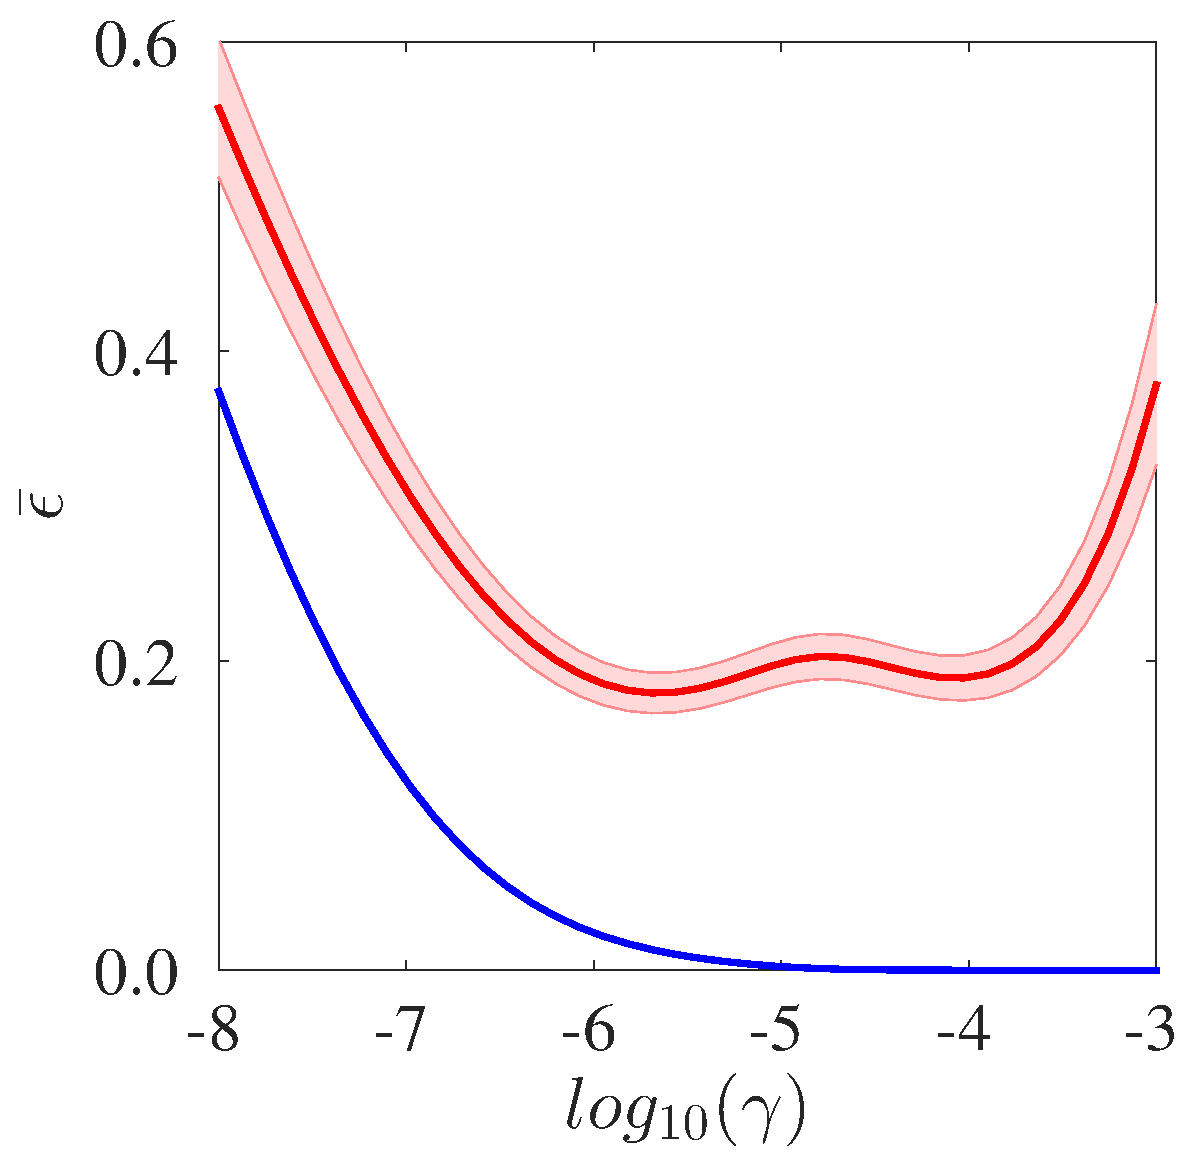
\includegraphics[height=6.75cm]{./images/regression/KRR_validationcurve_gamma.eps}	
	\caption{\label{fig:KRR_validationcurve} KRR validation curve (RBF kernel), with parameters are kernel parameter $ \gamma $ and regulartization parameter $ \lambda $. Red curves are for the prediction, while blue ones are for the training data}
\end{figure}

To plot validation and learning curves, the average normalized root mean square error (NRMSE) $ \bar{\epsilon} $ is used as the prediction error. $ \bar{\epsilon} $ represents an overall measure of the reconstruction accuracy. NRMSE is estimated between the reconstructed ($ \hat{\z}_t $) and reference ($ \z_t $) fields
\begin{equation}
\bar{\epsilon} = \left(\frac{ \sum\limits_{t} \sum\limits_{j\in \varmathbb{J}}(\hat{\mybold{z}}_{t,j}-\mybold{z}_{t,j})^2}{\sum\limits_{t} \sum\limits_{j\in \varmathbb{J}}\mybold{z}_{t,j}^2}\right)^{1/2}
\label{eq:NRMSE}
\end{equation} 
$ \varmathbb{J} $ is the considered set of points used to estimate the error. In the present case of isotropic turbulence, $ \varmathbb{J} $ contains all points in each plane.

Figure \ref{fig:RR_validationcurve} shows the validation and learning curve of RR model on the training set (blue) and validation set (red). The solid lines are the means, while a band of colors show the standard deviations of ten estimates of $ \bar{\epsilon} $ from ten folds. The validation curve (left) shows the model behavior for different $ \lambda $. For the training set, the model fits accurately the data when no or small regularization is imposed. This effect of overfitting is shown on the validation set, where higher errors are obtained. The model has also high variance, i.e. prediction errors vary strongly from one set to the other. The optimal value of $ \lambda \approx 100 $ is reached where the validation error is minimum. When a very strong regularization is imposed, errors on both training and validation sets increase, since all coefficients are shrunk toward zero. Errors will grow till their maximum value, which is the variance of the HR data. The learning curve (right) shows the effect of the training data size on the performance of the model (with optimal $ \lambda $). The figure shows that with larger training data, the prediction error on the validation set decrease sharply while this error on the training set gradually increase. With a good model and sufficiently large training data, these two curves will be very close. The curves also suggest that a larger dataset will lead to a better model in this case. 

KRR model parameters are optimized using the same validation curve. Different models come with different kernel parameters (recall table \ref{tab_basisfunctions}), together with the regularization parameter $ \lambda $. For RBF kernel, $ \gamma $ represents the kernel shape. Figure \ref{fig:KRR_validationcurve} shows that the optimal values of both $ \lambda $ and $ \gamma $ are both of the order of $ 10^{-5} $. For polynomial kernel, the polynomial order is to be tuned. The model with higher polynomial order will have lower bias but higher variance. An analogous procedure is used to find the optimal order of the polynomial fit, which is either 2 or 3 in general. 

\section{Concluding remarks}
In this chapter, regression models are used to reconstruct high resolution fields of an isotropic turbulence from low resolution measurements. The models seek a mapping function between low and high resolved fields. This function is learned from given training samples and used for prediction when only low-resolution measurements are available. 

Both linear and nonlinear models have been discussed. The ordinary least squares model is the simplest one and is widely used in the literature of turbulence. Since suffering from some critical limitations, notably overfitting and ill-conditioning, various regularization methods have been introduced. Both L2 and L1 penalty have been discussed. While L2 penalty reduces model variance by shrinking coefficients of irrelevant events, L1 forces them to zeros by slightly change the penalty term and offers some potential benefits. Nonlinear regression is another approach to improve OLS. Instead of assuming the underlying phenomenon is linear, it introduces nonlinearity by projecting input vectors to a fixed feature space before performing standard OLS. This nonlinearity helps in improving reconstruction accuracy, since assuming a linear relation between large and small scales of turbulence implies a big constraint on model performances. 

We have presented the procedure to optimize hyper-parameters of regression models. This step is crucial to ensure accurate predictions, since performances of all regression models (except OLS) depend on at least one parameter. The models are learned from the training data, but the performances are assessed on independent data only. Cross-validation is used to seek a compromise, the so-called bias-variance trade-off, from training data only. The dataset is virtually split into many subsets. The models are trained within some subsets, and their prediction generalized errors are estimated using the remaining sets. 

The optimal set of parameters is found using the validation curve and ten-fold cross validation technique. This curve shows the prediction errors on the validation set as a function of model parameters. It gives an idea of the optimal parameter range. Through all the tests, it is shown that the gradient of this curve near its minima is not very sharp, implying that a good estimate of these parameters can be achieved from the training data only. 

All model parameters are investigated. RR model is optimal when its regularization parameter $ \lambda $ is about $ 100 $. KRR model with RBF kernel is constructed with the optimal values of both $ \lambda $ and $ \gamma $ are of the order of $ 10^{-5} $. For polynomial KRR takes 2 or 3 as the optimal order of the kernel.
All such models will be used later in chapter \ref{chap_comparisons} to reconstruct high-resolution fields from low-resolution measurements and compared to other proposed methods.
\chapter{Learning coupled dictionaries}
\label{chap_dictionarylearning} 
This chapter describes an alternative approach to learn the relation between large and small scales of turbulence based on \textit{dictionary learning} methods. The approach finds coupled dictionaries to represent the low and high resolution turbulent fields and to reconstruct the missing small-scale information. This method has been applied successfully in image processing, and remains a very active research subject. It potentially outperforms regression models, which are sometimes too simplistic to represent the underlying phenomenon in turbulence. Indeed learned dictionaries could encode part of the physics of the flow. 

This chapter is organized as follows. First, different data representations are discussed, from predefined bases such as Fourier or wavelets to learned bases such as principal component analysis (PCA). Second, dictionary learning, a generalization of PCA, is discussed for the first time as a representation for turbulent fields. This section reviews also two algorithms to learn the dictionaries. Third, different approaches to learn coupled dictionaries of low and high resolution fields are presented. Last, the approach is tested on the DNS database of an isotropic turbulence presented in section \ref{sec:data_isotropic}. 

\section{From bases to dictionaries}
This section briefly reviews conventional representations of turbulent signals. Given a vector $ \x_t $, the main idea of all representation methods is to find a ``\textit{dictionary}'' $ \dict $, a set of basis functions or the so-called ``\textit{atoms}'' from which $ \x_t $ can be represented via a linear combination. This representation by coefficients $ \adictco_t $ is called a ``\textit{code}''. The representation can be exact:
\begin{equation}
\x_t = \dict \adictco_t
\end{equation}
or approximate:
\begin{equation}
 \x_t = \dict \adictco_t +\n_t
\end{equation}
where $ \n_t $ is an estimation noise term. Seeking the representation of the signal is an optimization problem to estimate the dictionary $ \dict $ and the code $ \adictco_t $. The dictionary can be mathematically predefined or learned from the data. The estimation of the coefficients $ \adictco_t $ can be very simple with very fast algorithms for predefined or orthogonal bases, or more complex with redundant dictionaries. 

\subsection{Predefined dictionaries}
Various types of dictionaries are studied to represent the data. They can be predefined \textit{a priori} such as the well-known Fourier transform, the group of \textit{wavelets} or \textit{curvelets} \citep{mallat1989theory,mallat1999wavelet}. These predefined transforms are easy to compute thanks to fast algorithms. Fourier transform aims at describing the signal via its frequency content by decomposing signals as an infinite series of sines and cosines. This transformation is localized in frequency but not in space/time. The constraint is overcome using wavelet transforms, replacing the sines and cosines by wavelet functions localized both in space/time and frequency. This property permits wavelets to better represent the signal with discontinuities or sharp spikes. In such cases, the representations are much more compact with wavelet functions than sines and cosines. This makes wavelets standard in signal compression, for example JPEG 2000 for images, while Fourier transform is mainly used for spectral analysis.

Representations using predefined bases suffer from some limitations. Fourier transform is limited to spectral analysis due to its localization in frequency. Wavelet transforms overcome this constraint by its carefully designed functions, which permit the localization both in space/time and frequency domain. The aim is to optimize the ``\textit{sparsity}'' of the representation, which is to minimize the number of basis functions to accurately represent the data. However, despite the large family of wavelets, all kinds of signals cannot be represented with high level of sparsity. Analogously for turbulence data, different flows or a single flow at various positions with respect to a wall can have significantly different physics, leading to signals with completely different properties.

\subsection{Adaptive dictionaries}
To further optimizing the representation, it is more appealing to learn dictionaries adaptively from the data \citep{bengio2013representation}. The first and most common method is the \textit{principal component analysis} (PCA). This approach learns a basis that maximizes the variance of the projected values. This is interesting for turbulence studies, since large scales of higher variances are of interest. This representation imposes orthogonal bases, which implies that the number of atoms is limited by the dimension of the input vectors. PCA is potentially subject to certain limitations due to this constraint. This chapter discusses the generalized version of PCA, which permits to learn a ``\textit{redundant}'' dictionary. The method is called \textit{dictionary learning}, which is widely used and remains an active research topic in image processing. It will be discussed further in this section before applying to the problem of turbulent field reconstruction. 

Adaptive dictionaries are useful in many applications \citep{tovsic2011dictionary}. The first one is \textit{dimension reduction} \citep{burges2010dimension}, which is useful to build models or visualize large amount of data. For modeling, high dimensional input variables potentially causes the problem of high variance as discussed in chapter \ref{chap_linearregression}, or intractable computation complexity. For visualization, it is a real constraint since the maximum number of dimensions one can observe and analyze is probably no more than three. The core idea is to project data onto a set of atoms in a dictionary. This projection is lossy, meaning that a certain amount of less informative variance is discarded. Another important application is to solve inverse problems such as super-resolution or denoising. These problems are very ill-posed and can not be solved directly by least-squares methods. A good representation of the data can play the role as a regularization term, making the problem easier to solve. The choice of a dictionary defines the space in which we search for solutions.

\section{Proper Orthogonal Decomposition (POD) as a representation of turbulent fields}
PCA \citep{jolliffe2002principal}, known also as \textit{Karhunen–Loève} transform, is commonly used in many fields of signal and image processing. It was first introduced in turbulence studies by \citet{lumley1967} under the name ``\textit{proper orthogonal decomposition}'' (POD). It is then used as a standard approach for dimensionality reduction, which is largely beneficial in large scales reconstruction, flow control and coherent structure studies. PCA decomposes a sequence of snapshots into a dictionary $ \dict $ to represent spatial structures, and a coefficient matrix $ \dictco $, to capture temporal dynamics. The works on coherent structures and flow information extraction focus on the dictionary $ \dict $ \citep{bonnet1994stochastic, gordeyev2000coherent}. Each atom $ \adict_i $, as ranked by its variance (an equivalent measure of the kinetic energy), represents the most energetic structures of the flow. Flow control and modeling works focus more on the use of projection coefficients $ \dictco $. After learning the fixed dictionary $ \dict $, independent of time, from given training fields, the temporal dynamics of the flow is presented in the projection coefficients $ \dictco $ only. The efforts to model and control the flow are reduced tremendously by considering only several coefficients of high-variance atoms. This property is beneficial for reduced-order modeling works in flow control and reconstruction of large-scale velocity fields \citep{ravindran2000reduced, ly2001modeling, taylor2004towards}.

To derive POD or PCA, let first denote a data matrix $ \X $ of size $ \dimsh \times \dimtl $ containing a sequence of $ \dimsh- $dimensional input vectors $ \x_t, t=1,2,...,\dimtl $,
\begin{equation}
\X \mydef \begin{bmatrix} \x_1, \x_2, ..., \x_\dimtl \end{bmatrix},
\end{equation} 
assumed centered \textit{a priori}:
\begin{equation}
\sum\limits_{t=1}^{\dimtl}\x_t = \mybold{0}
\end{equation}
From $ \X $, a dictionary $ \dict $ of size $ \dimsh \times \dimsh $ is estimated, which contains $ \dimsh $ atoms $ \adict_i \in \R ^\dimsh, i=1,2,...,\dimsh  $. The objective is to project $ \x_t $ onto a reduced-order subspace of dimension $ \dimtrunc \leq \dimsh $ while maximizing the amount of variance. This idea, when applying to turbulent fields where variance represents the kinetic energy, is interpreted as determining the most energetic structures among a sequence of snapshots. 

The first step is to find the most dominant basis function $ \adict_1  \in \R^\dimsh$, assuming $ \normtwo{\adict_1} = 1 $. Each input vector is projected onto this direction as $ \adict_1^\mytrans \x_t $. The variance of this projection is:
\begin{equation}
s_1 = \frac{1}{\dimtl} \sum\limits_{t=1}^{\dimtl}\left( \adict_1^\mytrans \x_t\right)^2 =  \adict_1^\mytrans \Sigma \adict_1
\end{equation}
where $ \Sigma  $ is the covariance matrix:
\begin{equation}
\Sigma = \frac{1}{\dimtl} X X^\mytrans
\end{equation}
The aim now is to find  $ \adict_1 $ such that $ s_1 $ is maximum, with the constraint that $ \normtwo{\adict_1} = 1$:
\begin{equation}
\adict_1 = \argmax_{\adict_1}{ \left\lbrace \adict_1^\mytrans \Sigma \adict_1 \right\rbrace } \:\:\:\:\:\: s.t \:\:\:\:\:\: \normtwo{\adict_1} = 1
\end{equation}
This optimization problem can be rewritten in an unconstrained manner by introducing a Lagrange multiplier $ \lambda_1 $:
\begin{equation}
\adict_1 = \argmax_{\adict_1}{ \left\lbrace \adict_1^\mytrans \Sigma \adict_1 + \lambda_1 \left(1-\adict_1^\mytrans \adict_1\right) \right\rbrace } 
\end{equation}
Setting the derivative with respect to $ \adict_1 $ to zero, one obtains:
\begin{equation}
\Sigma \adict_1 = \lambda_1 \adict_1
\end{equation}
which implies that $ \adict_1 $ is an eigenvector of $ \Sigma $, and $ \lambda_1 $ is the equivalent eigenvalue. Also, multiplying both side with $ \adict_1^\mytrans $, using $ \adict_1^\mytrans\adict_1=1 $, one has:
\begin{equation}
\adict_1^\mytrans \Sigma \adict_1 = \lambda_1
\end{equation}
The above expression implies that $ \lambda_1 $ is the variance of the projection onto $ \adict_1 $. This variance is maximized by selecting the maximum eigenvalue of the covariance matrix $ \Sigma $. This process is repeated to find the second basis of the dictionary $ \adict_2 $ such that it is orthogonal to the first one, i.e. $ \adict_1^{\mytrans}\adict_2=0 $. This is identical to find the second eigenvector corresponding to the second largest eigenvalue $ \lambda_2 $. The procedure of seeking all $ \dimsh $ bases is identical to eigenvalue decomposition and SVD of the covariance matrix $ \Sigma $. Sorting $ \dimsh $ eigenvalues in a descending order as $ \lambda_1 \geq \lambda_2 \geq ... \geq \lambda_\dimsh \geq 0 $, one obtains the dictionary, or codebook, learned from the training samples $ \X $ by putting the equivalent eigenvectors together as $ \dict \mydef \left[ \adict_1, \adict_2, ..., \adict_\dimsh \right] $. The projection matrix $ \dictco $ is found such that:
\begin{equation}
\X = \dict \dictco
\end{equation}


\section{Dictionary learning as a new representation}
Due to the orthogonality and variance maximization properties, PCA gains its success in many problems such as dimensionality reduction, low-order modeling and lossy compression. However, in solving different inverse problems, PCA is subject to several limitations. The number of atoms is at most the dimension of input vectors, leading to the ``limited expressiveness'' property \citep{tovsic2011dictionary}. The representation learned by PCA can be efficient for training data, but a good generalization is not guaranteed. It is desirable to ignore the constraint on the number of basis functions and learn a redundant dictionary. Due to the redundancy, the sparsity constraint can be imposed and play the role of the regularization to solve ill-posed inverse problems.

\subsection{Redundant dictionary and sparse representation}
Dictionary learning (DL) ignores the constraint on the number of basis functions, or atoms, permitting to find a \textit{redundant} (or \textit{overcomplete}) dictionary $ \dict \in \R^{\dimsh \times \dimdict} $ to represent the data. $ K $ is the number of atoms, and redundancy means that $ \dimdict $ is potentially larger than $ \dimsh $. These vectors are therefore not necessarily orthogonal. The companion of redundancy is sparsity, where the linear transformation matrix $ \dictco $ contains only a few nonzero coefficients. The representation then relies on the duality between redundancy and sparsity, which will be discussed further in this section. With more atoms, the representation using dictionary learning is expected to be more adaptive to the signal and to better represent new data. This is the reason why the approach often gives the state-of-the-art results in most inverse problems in image processing \citep{elad2010on,yang2010image}.

The problem of representing data $ \X $ using the redundant dictionary $ \dict $ and sparse coefficients $ \dictco $ includes two alternating optimization problems. The first one is to estimate the projection coefficients $ \dictco $. PCA, with the orthogonality among atoms, simply estimates $ \dictco $ by dot products. Dictionaries, which are not necessarily orthogonal, can have more atoms than the dimension ($ \dimdict > \dimsh $). There are potentially many matrices $ \dictco $ such that $ \X = \dict \dictco $. The sparsity constraint, meaning that $ \dictco $ has a minimal number of nonzero coefficients, is imposed to make the solution unique. The representation of $ \X $ becomes approximate, i.e. $ \X \approx \dict \dictco $. Finding $ \dictco $ becomes an optimization problem of the form:
\begin{equation}
\dictco = \argmin_{\dictco}{\normp{\dictco}} \quad s.t. \quad \X = \dict \dictco
\end{equation}
or re-arranged in the form of a regularized cost function as in chapter \ref{chap_linearregression}:
\begin{equation}
\dictco = \argmin_{\dictco}{\normtwo{\X - \dict \dictco} + \lambda \normp{\dictco}}
\end{equation}
The common \textit{$ \ell^p $ norm} $ \normp{.} $ is with $ 0 \leq p \leq 1 $. Solving the problem with the $ \ell^0 $ norm, i.e. counting the number of nonzero coefficients, leads to orthogonal matching pursuit (OMP) \citep{tropp2007signal}, while solving with the $ \ell^1 $ norm, summing the absolute values of the coefficients, leads to LASSO as discussed in chapter \ref{chap_linearregression}. Least Angle Regression (LARS) \citep{efron2004least} is sometimes used as another efficient algorithm to solve $ \ell^1 $ penalty problems and gives results very similar to LASSO. These regularizations help selecting a limited number of atoms that best approximate the input $ \X $. The second problem is the choice of the dictionary, which is solved by efficient algorithms discussed in the next section.

\subsection{Dictionary learning methods}
Many algorithms have been proposed to learn the dictionary from data, starting with gradient descend method \citep{olshausen1996emergence}, then K-SVD \citep{aharon2006ksvd}, feature-sign approach \citep{lee2006efficient} and online dictionary learning \citep{mairal2010online}. This section reviews some of those that are used later in this chapter. 

\subsubsection{Alternate optimization}
Dictionary learning is an alternate optimization problem to search the redundant dictionary $ \dict $ and the sparse matrix $ \dictco $. The approach has started by using a gradient descent approach \citep{olshausen1996emergence}. It has recently gained popularity thanks to the progress in solving regularized optimization problems with $ \ell^p $ penalty \citep{tibshirani1996regression, donoho2003optimally, efron2004least, donoho2012sparse}. One of the first efficient dictionary learning approach is the \textit{method of optimal directions} (MOP) \citep{engan1999method} where $ \dict $ and $ \dictco $ are estimated by solving:
\begin{equation}
(\dict, \dictco) = \argmin_{\dict, \dictco} \normtwo{\X - \dict \dictco} \subjectto \normzero{\adictco_t} < \dimtrunc \quad \forall t
\end{equation}
$ \dimtrunc $ is the sparsity constraint- the maximum number of nonzero coefficients. This optimization problem is  combinatorial and highly non-convex. The search for a local minimum is done by alternating two steps. With a fixed dictionary $ \dict $, the \textit{sparse coding} step finds the representation of the input vectors by solving:
\begin{equation}
\dictco = \argmin_{\dictco} \left\lbrace \normtwo{\X - \dict\dictco} + \lambda \normp{\dictco}\right\rbrace
\end{equation}
This step uses OMP for $ \ell^0 $ penalty and LASSO or LARS for $ \ell^1 $ penalty. The \textit{dictionary update} step re-estimates $ \dict $ with fixed $ \dictco $ via the Moore-Penrose pseudo-inverse:
\begin{equation}
\dict = \X \dictco^\mypseudo = \X \dictco^\mytrans (\dictco \dictco^\mytrans)^{-1}
\end{equation}
This scheme converges rapidly after some iterations, but requires complex matrix inversion, which is not efficient in most cases \citep{aharon2006ksvd}. 
\subsubsection{K-SVD}
The \textit{K-SVD} algorithm was proposed later by \citet{aharon2006ksvd} and rapidly gained its popularity. The \textit{dictionary update} is done by a block-relaxation approach. Instead of inversing the matrix, the algorithm updates each atom in an efficient way by generalizing the \textit{k-means} clustering method \citep{bishop2006pattern}. The $ k- $th atom is estimated by minimizing a quadratic error:
\begin{equation}
	\left\lbrace \adict_k, \adictco_k \right\rbrace = \argmin_{\adict_k, \adictco_k} \normtwo{E_k \: - \: \adict_k \adictco_k^\mytrans}
\end{equation} 
where $  E_k $ is defined as the residual matrix:
\begin{equation}
E_k \mydef \X_k \: - \: \sum_{j\neq k} \left(\adict_j \adictco_j^\mytrans \: - \: \adict_k \adictco_k^\mytrans\right)
\end{equation}
where $ \X_k $ gathers examples $ \x_t $ using $ \adict_k $ in their representation. The update of both $ \adict_k $ and $ \adictco_k $ is done simultaneously via a rank-1 approximation, i.e. considering only the first eigenvector of $ E_k $ after performing a SVD.

\subsubsection{Online dictionary learning (ODL)}
K-SVD algorithm has certain constraints, mainly with a potential local minimum while iteratively learning the dictionary \citep{rubinstein2010dictionaries}. The algorithm is also limited to small numbers of samples due to its computational cost. Online dictionary learning (ODL) has been proposed by \citet{mairal2010online} to learn $ \dict $ from massive datasets. The use of stochastic gradient descent to update the dictionary for each example (or a group of them), and LARS algorithm for sparse coding, permits the learning over millions of samples. Algorithm \ref{algo_ODL} summarizes this approach.

\begin{algorithm}[t]
\caption{Online dictionary learning algorithm by  \citet{mairal2010online}} \label{algo_ODL}
\begin{algorithmic}[1]
	\State Input: 
	\begin{itemize}
		\item a set of $ \mathcal{S}(\x) $ of $\dimtl $ input variable $ \x_t \in \R^\dimsh$;
		\item $\lambda \in \R $ : regularization parameter ($ \lambda \geq 0 $)
		\item $ \dict_0 \in \R^{\dimsh \times K}$: initial dictionary
	\end{itemize}
	\State $ \mathbf{G}_0 \gets  0$, $ \mathbf{H}_0 \gets 0 $
	\For {$ t = 1, 2, ..., \dimtl$}
		\State Draw $ \x_t $ from $\mathcal{S}(\x)$
		\State Sparse coding:
		\begin{equation}
			\adictco_t = \argmin_{\adictco \in \R^K} \left\lbrace \x_t - \dict_{t-1}\adictco +\lambda \normone{\adictco}\right\rbrace
		\end{equation}
		\State $ \mathbf{G}_t \gets \mathbf{G}_{t-1}+\adictco_t \adictco_t^\mytrans$
		\State $ \mathbf{H}_t \gets \mathbf{H}_{t-1}+\adictco_t \x_t^\mytrans$
		\State Update $ \dict_t $:
		\begin{equation}
			\begin{split}
			\dict_t = & \argmin_{\dict \in \mathcal{C}} \left\lbrace \frac{1}{t} \sum\limits_{i=1}^{t}\frac{1}{2} \normtwo{\x_i - \dict\adictco_i} + \lambda \normone{\adictco_i} \right\rbrace \\
			=& \argmin_{\dict \in \mathcal{C}} \left\lbrace \frac{1}{t} \sum\limits_{i=1}^{t}\frac{1}{2} \mytrace{\dict^\mytrans\dict \mathbf{G}_t} - \mytrace{\dict^\mytrans \mathbf{H}_t} \right\rbrace
			\end{split}
		\end{equation}
	\EndFor
	\State Return $ \dict_\dimtl $
\end{algorithmic}
\end{algorithm}

\section{Learning coupled dictionaries}
\label{joint_learning}
In this section, DL is used to solve the problem of reconstructing HR fields from LR ones. The approach is inspired by the \textit{single image super-resolution} application \citep{yang2010image,yang2012coupled,zeyde2012single}, i.e. estimating HR images with finer details from LR ones. The approach jointly learns coupled dictionaries at LR and HR from given training samples. These dictionaries are forced to represent the data using the same coefficients. In the prediction phase, the projection coefficients are estimated from the LR images and then combined with the learned HR dictionary to reconstruct the HR images. 

\subsection{Patch-based approach}
\label{subsec:patch_based_estimation}
\begin{figure}
\centering
	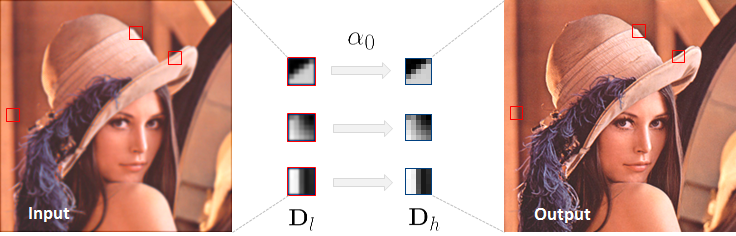
\includegraphics[width=0.9\textwidth]{./images/DL/ScSR.png}
	\caption{\label{fig:ScSR} An example of single image super-resolution using coupled dictionary learning and patch-wise approach. Photo credit: \citet{yang2010image}.}
\end{figure}

DL requires a sparse coding step, i.e. solving the $ l^1 $-penalty optimization problem. The computation complexity is $ \mathcal{O}(\dimsh^3+\dimtl\dimsh^2) $ \citep{efron2004least}, where $ \dimsh $ is the dimension of the fields and $ \dimtl $ is the number of samples. Since $ \dimsh \gg \dimtl$ in most cases, the complexity is $ \mathcal{O}(\dimsh^3) $, which is a very heavy procedure. The computation is therefore intractable with the whole field. To overcome this difficulty, the ``\textit{patch-wise}'' approach uses small patches instead of the whole fields. These patches are extracted from the original fields at all positions by moving pixel-by-pixel in both horizontal and vertical directions. Let $ \dimptl $ be the total number of patches, and $ \dimpsh $ be their dimension ($\dimptl \gg \dimpsh $), the computation complexity becomes $ \mathcal{O}(\dimptl\dimpsh^2) $, which is tractable when $ \dimpsh $ is small. In the reconstruction phase, since one pixel belongs to several intersecting patches, the estimated field is reconstructed by aggregating all possible estimates of each pixel after putting them back into the whole scene.

The path-wise approach comes with several advantages. First, it localizes the information. A shared dictionary can be learned to represent all type of images with different contents. Second, it reduces tremendously the computation. Standard images are of dimension few millions, while typical patch sizes are around $ 8 \times 8 $, which is a few orders of magnitude smaller. Last, since the learning is on small patches, the number of samples required for the algorithm to converge is much smaller. From a single image, millions of small patches can be extracted for learning. Working with the original image, the number of training samples is necessary at least one order of magnitude higher than its dimension, which is already millions of pixels. 

To formulate the patch-based approach, let $ \z_t \in \R^{\dimsh} $ be a snapshot of a high-resolution field as a column vector. The operator $ \extracthigh{k}:\R^{\dimsh} \mapsto \R^{\dimpsh} $ is to extract the 2D patch and put them in a lexicographical order to form a column vector $ \patchhigh{k} \mydef \extracthigh{k} \z_t \in \R^\dimpsh $, where $ \dimpsh $ is the size of 2D patches $ \patchhigh{k} $. If the overlapping is such that all patches are translated pixel-by-pixel, the total number of patches is $ \left( \sqrt{\dimsh} - \sqrt{\dimpsh} + 1 \right)^2 $. The reconstruction of the whole image is done as:
\begin{equation}
\hat{\z}_t= \left[ \sum\limits_{k} \left(\extracthigh{k}\right)^{\mytrans}\extracthigh{k}\right]^{-1}\sum\limits_{k} \left(\extracthigh{k}\right)^{\mytrans}\hat{\mybold{p}}_h^k
\end{equation}
where $ \hat{\mybold{p}}_h^k $ and $ \hat{\z}_t $ are the estimates of the reference $ \patchhigh{k} $ and $ \z_t $ respectively. The term $ \left(\extracthigh{k}\right)^{\mytrans}: \R^{n} \mapsto \R^{\dimsh}$ puts the equivalent patch into the global 2D scene and zero-pad elsewhere. The term $ \left(\extracthigh{k}\right)^{\mytrans}\extracthigh{k} $ just counts the number of estimates for each pixels. Its inversion plays the role of a normalization factor. In practice, the whole process is done by estimating each pixel as its mean or median of all estimates from all patches that it belongs to. 

\subsection{The approach}
\label{sec:chap3_theapproach}
Let assume that small patches from the field can be represented as a linear combination of several atoms from the learned dictionary. This assumption is the so-called ``\textit{Sparse-Land}'' prior \citep{zeyde2012single}. The idea is to learn coupled dictionaries by imposing that the representation coefficients are the same at low and high resolution. The following section recalls the main ideas. More details can be found in \citet{zeyde2012single}.

Suppose that $ \z_t \in \R^{\dimsh}$ is the true high resolution velocity field. The corresponding low-resolution field $ \y_t \in \R^{\dimsl} $ $(\dimsl < \dimsh) $ is obtained as:
\begin{equation}
\y_t = \Sub_s\LPF_s\z_t + \mybold{v}_t
\label{eq:DL_approach1}
\end{equation}
where $ \mybold{v}_t $ is a random noise, $ \LPF_s $ is an anti-aliasing low-pass filter, and $ \Sub_s $ is a subsampling operator. The presence of $ \LPF_s $ is to avoid the problem of aliasing when subsampling the field. In the case of direct subsampling, this filter is omitted from the above model. The goal is to find a HR estimate $ \hat{\z}_t $ containing both large and small scales. The most naive and simple idea is to interpolate from $ \y $, i.e. $ \hat{\z}_t = \Interp_s\y_t \in \R^{\dimsh}$. However, it will give no access to small-scale information above the cutoff frequency defined by the low-resolution grid. The coupled dictionary approach permits to learn small scales from training data and uses it for the reconstruction. 

DL uses the patch-based approach, where the couples of LR and HR patches are extracted from the LR and HR fields respectively. Let $ \patchhigh{k} = \mathcal{R}_h^k \z_t \in \R^\dimpsh $ be the $ k-${th} HR patch. By assuming the Sparse-Land model for high and low resolution training fields, each patch can be estimated as a linear combination of atoms in a dictionary:
\begin{equation}
\patchhigh{k} = \dict_h \adictco^k + \mybold{\epsilon}^k
\label{eq:DL_approach2}
\end{equation} 
where $ \dict_h  \in  \R^{\dimpsh \times K}$ is the HR dictionary, $ \adictco^k \in \R^K$ is the coefficient vector and $ \mybold{\epsilon}^k $ is the reconstruction error. The dictionary is redundant ($ K > \dimpsh $) and the coefficients are sparse ($ \Arrowvert \adictco^k \Arrowvert_0 < \dimtrunc $), with the sparsity constraint $ \dimtrunc \ll K $. The corresponding LR patch $ \patchlow{k} \in \R^\dimpsl $ is: 
\begin{equation}
	\patchlow{k} = \extractlow{k} \y_t = \extractlow{k} \Sub_s\LPF_s\z_t + \extractlow{k}\mybold{v}_t
\label{eq:DL_approach3}
\end{equation}	
$ \extractlow{k} $ is just an extraction operator, and $ \Sub_s\LPF_s $ is a transformation operator going from HR to LR fields. Since $ \Sub_s $ and $ \LPF_s $ are spatially independent operators, there exit local $ \Sub_s^{loc} $ and $ \LPF_s^{loc} $ that transform HR to LR patches:
\begin{equation}
	\patchlow{k} =  \Sub_s^{loc}\LPF_s^{loc}\patchhigh{k} + \mybold{v}_\ell^k
	\label{eq:DL_approach4}
\end{equation}  
where $ \mybold{v}_\ell^k $ is a random noise of the same dimension as the LR patches. From equations \ref{eq:DL_approach2} and \ref{eq:DL_approach4}, one can write:
\begin{equation}
\begin{split}
	\patchlow{k} &= \Sub_s^{loc}\LPF_s^{loc}\dicthigh \adictco^k + \Sub_s^{loc}\LPF_s^{loc}\mybold{\epsilon}^k + \mybold{v}_\ell^k \\
				 &= \Sub_s^{loc}\LPF_s^{loc}\dicthigh \adictco^k + \tilde{\mybold{v}}_\ell^k
\end{split}
\label{eq:DL_approach5}	
\end{equation}
where $ \tilde{\mybold{v}}_\ell^k \mydef \Sub_s^{loc}\LPF_s^{loc}\mybold{\epsilon}^k + \mybold{v}_\ell^k$ is also a random noise term. Denoting $ \dictlow \mydef \Sub_s^{loc}\LPF_s^{loc}\dicthigh  $, the above equation illustrates that there exists also a Sparse-Land model for LR patches. These models for LR and HR patches also share the same sparse coefficient $ \adictco^k $. The LR dictionary is also a downsampled version of the HR one.

\subsection{Joint learning methods}
\label{sec:joint_learning_methods}
In practice, $ \Sub_s\LPF_s $ or $ \Sub_s^{loc}\LPF_s^{loc} $ are usually not given. \citet{yang2010image} has addressed this problem by proposing the approach to jointly learn coupled dictionaries. \citet{zeyde2012single} follow the main idea with some modifications. All approaches contains two main steps: \textit{learning phase} and \textit{reconstruction phase}. The learning phase can be done \textit{offline}, i.e. training \textit{a priori} from the data. With learned dictionaries, the reconstruction phase can be \textit{online}.

Given the training HR velocity fields $ \z_t \in \R^{\dimsh} $, corresponding LR fields are virtually extracted as $ \y_t=\Sub_s\LPF_s\z_t \in \R^{\dimsl}$. Couples of LR and HR patches $ \left\lbrace  \patchlow{k},\patchhigh{k}  \right\rbrace $ are extracted from the training fields as $ \patchlow{k}= \extractlow{k} \y_t\in  \R^\dimpsl $ and $ \patchhigh{k}= \extracthigh{k} \z_t\in  \R^\dimpsh $, where $ \dimpsl $ and $ \dimpsh $ are the size of LR and HR patches respectively, and $ \dimpsh/\dimpsl = \dimsh / \dimsl $. Let $ \mathbf{P}_\ell $ and $ \mathbf{P}_h $ denote matrices of all LR and HR patches:
\begin{equation}
	\begin{split}
		\mathbf{P}_\ell&=\left[\patchlow{1} \:\: \patchlow{2} \:\: ... \:\: \patchlow{\dimptl}\right]_{\dimpsl \times \dimptl} \\
		\mathbf{P}_h&=\left[\mybold{p}_h^1 \:\: \mybold{p}_h^2 \:\: ... \:\: \mybold{p}_h^{\dimptl}\right]_{\dimpsh \times \dimptl}
	\end{split}
	\label{eq:jointlearning1}
\end{equation}
where $ \dimptl $ is the total number of patches, and $ \dimptl = \left(\sqrt{\dimsl} - \sqrt{\dimpsl} + 1\right)^2 \times \dimtl$ at most, where $ \dimtl $ is the number of training planes. The LR patches are collected by one-pixel overlapping, while HR ones are obtained by overlapping $ \dimpsh/\dimpsl $ pixels to ensure the same number of LR and HR patches. Coupled dictionaries $ \left\lbrace \dicthigh ,\dictlow  \right\rbrace $ are learned from the coupled training patches $ \left\lbrace \mathbf{P}_h ,\mathbf{P}_\ell  \right\rbrace $ imposing to share the same sparse representation:
\begin{equation}
\begin{cases}
	\mathbf{P}_h \approx \dicthigh \dictco\\
	\mathbf{P}_\ell \approx \dictlow \dictco\\
\end{cases}
\end{equation}            
The first learning approach is proposed by \cite{yang2010image}, which aims at solving an optimization problem:
\begin{equation}
\left\lbrace \dicthigh ,\dictlow, \dictco  \right\rbrace = \argmin_{\dicthigh ,\dictlow ,A} \left\lbrace \frac{1}{\dimpsh} \Vert \mathbf{P}_h-\dicthigh \dictco\Vert^2_2 + \frac{1}{\dimpsl} \Vert \mathbf{P}_\ell-\dictlow \dictco\Vert^2_2 + \lambda_1 \left( \frac{1}{\dimpsh}+\frac{1}{\dimpsl} \right) \Vert \dictco \Vert_1 \right\rbrace
\label{eq:jointlearning2}
\end{equation}
$ \dictco $ is the shared sparse coefficients, which ensures a compromise between small reconstruction errors of patches and sparsity constraint. The two normalization terms $ 1/\dimpsl  $ and $ 1/\dimpsh $ are to balance the two mean-square error terms. The above cost function can be re-written as:
\begin{equation}
\dict = \argmin_{\dict,\dictco} \left\lbrace \Vert \mathbf{P}-\dict \dictco\Vert^2_2 + \lambda_1 \Vert \dictco \Vert_1 \right \rbrace
\label{eq:jointlearning3}
\end{equation}
where
\begin{equation}
\mathbf{P}= \begin{bmatrix} \frac{1}{\sqrt{\dimpsh}}\mathbf{P}_h \\ \frac{1}{\sqrt{\dimpsl}}\mathbf{P}_\ell \end{bmatrix}, \:\: \dict= \begin{bmatrix} \frac{1}{\sqrt{\dimpsh}}\dicthigh  \\ \frac{1}{\sqrt{\dimpsl}}\dictlow  \end{bmatrix}
\label{eq:jointlearning4}
\end{equation}
This problem can be solved using the standard DL algorithms.

The second approach is proposed by \citet{zeyde2012single}, which contains a direct model to estimate the HR dictionary. The LR dictionary is first learned from LR patches:
\begin{equation}
\left\lbrace \dictlow ,\dictco \right\rbrace =\argmin_{\dictlow, \dictco}  \left\lbrace \normtwo{\mathbf{P}_\ell-\dictlow \dictco} + \lambda_1\Vert \dictco \Vert_1 \right \rbrace
\label{eq:jointlearning5}
\end{equation}
Assuming that the representation of HR patches $ \mathbf{P}_h $ via the HR dictionary $ \dicthigh  $ will share the same sparse code $ \dictco $, HR dictionary is estimated as:
\begin{equation}
\dicthigh  = \argmin_{\dicthigh } \left\lbrace \Vert \mathbf{P}_h-\dicthigh \dictco\Vert^2_2  \right \rbrace
\label{eq:jointlearning6}
\end{equation}
for which the solution is easy to obtain by a pseudo-inverse:
\begin{equation}
\dicthigh =\mathbf{P}_h \dictco^{\dagger}=\mathbf{P}_h\dictco^{\mytrans}(\dictco\dictco^{\mytrans})^{-1}
\label{eq:jointlearning7}
\end{equation}

As originally proposed for image super-resolution where sharp edges are important, \citet{yang2010image,yang2012coupled,zeyde2012single} use different pre-processing techniques before learning coupled dictionaries. Interpolated images $ \Interp_s\y_t $ of the same dimension as HR ones are considered as LR images. \citet{yang2010image,yang2012coupled} couple HR patches, i.e. $ \patchhigh{k}=\extracthigh{k}\z_t$,  with the derivatives of interpolated LR images $ \varmathbb{F} \Conv \Interp_s\y_t $. The operator $ \Conv $ is the convolution operator. These derivatives are obtained from the convolution of four different 1D kernels $ \varmathbb{F} $ of first and second order:
\begin{equation}
	\left[ \begin{matrix} -1 & 0 & 1 \end{matrix} \right] , \:\: \left[ \begin{matrix} -1 & 0 & 1 \end{matrix} \right]^{\mytrans} , \:\: \left[ \begin{matrix} 1 & 0 & -2 & 0 & 1 \end{matrix} \right] , \:\: \left[ \begin{matrix} 1 & 0 & -2 & 0 & 1 \end{matrix} \right]^{\mytrans}
\label{eq:jointlearning8}
\end{equation}
LR patches are then extracted as $\patchlow{k}= \extracthigh{k}(\varmathbb{F} \Conv \Interp_s\y_t) $. \citet{zeyde2012single} couples the same features $ \varmathbb{F} \Conv \Interp_s\y $, but with the residual between HR and interpolated images, i.e. $ \patchhigh{k}=\extracthigh{k}(\z_t-\Interp_s\y_t) $. Moreover, the dimension is reduced using PCA, which corresponds to an adaptive low-pass filter. This step in practice is important, since applying the four filters to low resolution fields bring redundant and superfluous information and lead to unnecessary heavy computation. 

\begin{table}
	\caption{\label{tab:DLapproaches}
	Notations for three different methods of coupled dictionaries learning as proposed by \citet{yang2010image,zeyde2012single}. The dimension of LR and HR patches are $ \dimpsl $ and $ \dimpsh $ respectively.}
	\vspace{.5cm}
	\centering
	\begin{tabular}{ccccccc} 
		\toprule \multirow{2}{*}{Notation}&\multicolumn{1}{c}{}&\multicolumn{2}{c}{Patch extraction}&\multicolumn{1}{c}{}&\multicolumn{2}{c}{Patch dimension}\\
		\cmidrule{3-4} \cmidrule{6-7}
	 & & {LR} & {HR} & & {LR} & {HR} \\
		\midrule 
		SR1  &&  $ \extractlow{k} \Sub_s\LPF_s\z_t $  & $ \extractlow{k} \z_t $ && $ \dimpsl $ & $ \dimpsh $\\
		SR2  &&  $ \extractlow{k} \Interp_s\Sub_s\LPF_s\z_t $  & $ \extractlow{k} \z_t $ && $ \dimpsh $ & $ \dimpsh $\\
		SR3  &&  $ \extractlow{k} \extracthigh{k}(\varmathbb{F} \Conv \Interp_s\y_t) $  & $ \extractlow{k} \left\lbrace \z_t - \Interp_s\y_t\right\rbrace$ && $ 4\dimpsh $ & $ \dimpsh $ \\
		\bottomrule
	\end{tabular}
\end{table}

Based on the above works by \citet{yang2010image,zeyde2012single}, we study three different approaches, namely ``\textit{SR1}'',``\textit{SR2}'' and ``\textit{SR3}'', to learn coupled dictionaries. Descriptions of LR and HR patches with their sizes are summarized in table \ref{tab:DLapproaches}. The dimension of LR patches when using derivatives is $ 4 \dimpsh $; However in practice, it is reduced significantly via PCA while retaining $ 99.9 \% $ of energy content.

\subsection{Reconstruction using learned dictionaries}
Having the coupled dictionaries at hand and given a LR field $ \y^\ext $, the objective is to reconstruct the HR $ \z^\ext $. The superscript ``$ \ext $'' stands for ``\textit{external}'', meaning outside of the training planes. First, all LR patches $ \mathbf{P}^\ext_\ell$ are extracted from $ \y^\ext $ with the overlapping of one pixel. $ \mathbf{P}^\ext_\ell$ is then centered by removing the mean of each patch $ m_l $. Next, the sparse code $ \dictco $ are estimated by solving the regularized least-squares problem:
\begin{equation}
\dictco^\ext =\argmin_{\dictco^\ext} \left\lbrace \Vert \mathbf{P}_\ell-\dictlow \dictco^\ext\Vert^2_2 + \lambda_2 \Vert \dictco^\ext \Vert_1 \right\rbrace 
\label{eq:DLrec1}
\end{equation}
HR patches are estimated using this shared code and putting back the mean $ m_l $:
\begin{equation}
\hat{\mathbf{P}}^\ext_h = \sqrt{\frac{\dimpsh}{\dimpsl}} \dicthigh \dictco^\ext + m_l
\label{eq:DLrec2}
\end{equation}
Finally, the HR field is reconstructed by solving an optimization problem:
\begin{equation}
\hat{\z}^\ext = \argmin_{\z^\ext} \left\lbrace\sum\limits_{k} \Arrowvert \extracthigh{k}\hat{\z}^\ext- \hat{\mybold{p}}_h^k\Arrowvert^2_2 \right\rbrace
\label{eq:DLrec3}
\end{equation}
This problem aims to find the best compromise between all estimates, and the closed-form least-squares solution is:
\begin{equation}
\hat{\z}^\ext= \left[ \sum\limits_{k} \left(\extracthigh{k}\right)^{\mytrans}\extracthigh{k}\right]^{-1}\sum\limits_{k} \left(\extracthigh{k}\right)^{\mytrans}\hat{\mybold{p}}_h^k
\label{eq:DLrec4}
\end{equation}
This is the overlapping procedure as discussed in section \ref{subsec:patch_based_estimation}. A pseudo algorithm of the whole process including the learning and reconstruction phases is summarized in algorithm \ref{algo_SR}.

\begin{algorithm}
\caption{Coupled dictionary learning for reconstruction of high-resolution fields from low-resolution ones} \label{algo_SR}
\begin{algorithmic}[1]
	\State \textbf{Input}:
	\begin{itemize}
		\item training high-resolution fields $ \left\lbrace \z_t \right\rbrace, t=1,2,...,\dimtl$
		\item testing low-resolution field $ \y^\ext $
	\end{itemize}
	\State \textbf{Step 1}: \textit{Learning phase} (offline)
	\begin{itemize}
		\item Extract virtual low-resolution fields the same way as $ \y^\ext $ is recorded: 
		\begin{equation}
			\label{eq:algo_SR_1}
			\y_t \mydef \Sub_s\LPF_s\z_t + \mybold{v}_t
		\end{equation}
		\item Extract and join coupled patches $ \left\lbrace \mathbf{P}_l,\mathbf{P}_h \right\rbrace $ from the fields $ \left\lbrace \y_t, \z_t \right\rbrace, t=1,2,...,\dimtl $:
		\begin{equation}
			\label{eq:algo_SR_2}		
			\mathbf{P} \mydef \left[ \frac{1}{\sqrt{\dimpsh}}\mathbf{P}_h ; \frac{1}{\sqrt{\dimpsl}}\mathbf{P}_\ell \right]
		\end{equation}
		\item Learn the joint dictionary $ \dict \mydef \left[\frac{1}{\sqrt{\dimpsh}}\dicthigh; \frac{1}{\sqrt{\dimpsl}}\dictlow \right] $ as:
		\begin{equation}
			\label{eq:algo_SR_3}		
			\left(\dict, \dictco\right) = \argmin_{\dict,\dictco} \left\lbrace \Vert \mathbf{P}-\dict \dictco\Vert^2_2 + \lambda_1 \Vert \dictco \Vert_1 \right\rbrace
		\end{equation}
	\end{itemize}	
	\State \textbf{Step 2}: \textit{Reconstruction phase} (online)
	\begin{itemize}
		\item Extract LR patches: $ \mathbf{P}_\ell ^\ext \in \R^{\dimpsl \times \dimptl}$ from $ \y^\ext $
		\item Estimate the sparse code:
		\begin{equation}
			\label{eq:algo_SR_4}		
			\dictco^\ext = \argmin_{\dictco^\ext} \left\lbrace \Vert \mathbf{P}_\ell^\ext-\dictlow \dictco^\ext\Vert^2_2 + \lambda_2 \Vert \dictco^\ext \Vert_1 \right\rbrace 
		\end{equation}
		\item Reconstruct HR patches $ \hat{\mathbf{P}}_h^\ext = \dicthigh\dictco^\ext  \in \R^{\dimpsh \times \dimptl} $
	\end{itemize}
	\State \textbf{Output:} Reconstruct HR field $ \z^\ext $ from $  \hat{\mathbf{P}}_h^\ext  $ by overlapping.
\end{algorithmic}
\end{algorithm}
 
\section{Dictionary learning for isotropic turbulence fields}
The section applies dictionary learning approach to the DNS database of the isotropic turbulence discussed in chapter \ref{sec:data_isotropic}. This data is chosen because the fields are periodic, isotropic and homogeneous. These properties will facilitate all computations and the handling of boundary conditions. Two main problems are addressed. First, the efficiency of the representation using dictionary learning will be studied, comparing with other approaches such as wavelet transform or PCA. Second, the coupled dictionaries approach is discussed to solve the problem of reconstructing HR velocity fields from LR measurements. 

To compare with other approaches, we consider a similar configuration as in chapter \ref{chap_linearregression} to study regression models. The reference HTHS data is subsampled to obtain the measurements of HTLS $ \{\y_t\} $ and LTHS $ \{\x_t\} $ (see figure \ref{fig:space-time_measurements}). The subsampling ratios are $ \dimsh/\dimsl = 4 \times 4$ in space and $ \dimth/\dimtl = 6 $ in time, corresponding to a moderate amount of energy losses in every directions. We will use $ \{\x_t\} $ only for the training, then uses $ \{\y_t\} $ to predict $ \{\z_t\} $.

\subsection{On the choice of parameters}
\label{subsec:DL_choice_params}
\begin{table} 
	\caption{\label{tab:DLparams}
	Set of parameters for coupled dictionaries approach (notations are consistent with Algorithm \ref{algo_SR}): sparsity constrains $ \lambda_1 $ for learning and $ \lambda_2 $ for reconstruction; dimension of LR patches $ \dimpsl $ and HR patches $ \dimpsh $; number of atoms $ \dimdict $; number of training patches $ \dimptl $ }
	\vspace{.5cm}
	\centering
	\begin{tabular}{cccccc} 
		\toprule
		{$\lambda_1$} & {$\lambda_2$} & {$\sqrt{\dimpsl}$} & {$\sqrt{\dimpsh}$} & {$\dimdict$} & {$ \dimptl $} \\ 
		\midrule 
		$ 0.1 \sim 0.2 $  &  $ 10^{-5} $  & 4  & 16 & $ 2(\dimpsl \times \dimpsh) $ & $~ 10^5 $ \\ %\addlinespace
		\bottomrule
	\end{tabular}
\end{table}

Results in the following sections are obtained with a consistent set of parameters presented in table \ref{tab:DLparams}. Notations are consistent with the algorithm \ref{algo_SR} to learn coupled dictionaries. This section briefly discusses these choices.

The first set of parameters are sparsity constraints $ \lambda_1 $ and $ \lambda_2 $. For the learning phase, $ \lambda_1 $ is about $ 0.1 \sim 0.2 $ to learn either the coupled dictionaries in equation \ref{eq:jointlearning2} or the LR dictionary in equation \ref{eq:jointlearning5}. This constraint imposes that the reconstruction of training patches uses only $ 10\sim15 $ nonzero coefficients in average, corresponding to the sparsity level of $ 0.90\sim0.95 $ (only $ 5 \sim 10\% $ coefficients are nonzero). As will be seen latter in figure \ref{fig:Sparsity_vs_NRMSE}, this is a strong constraint. However, decreasing $ \lambda_1 $, i.e. reducing the sparsity level, downgrades reconstruction results of coupled dictionaries. This is probably the \textit{overfitting} problem discussed in chapter \ref{chap_linearregression}. With small $ \lambda_1 $, the dictionaries represent well the training data but with a poor generalization capability. For reconstruction phase, $ \lambda_2 $ is chosen to be close to zero. In such case, the sparsity level of $ \dictco^\ext $ in equation \ref{eq:algo_SR_4} is very low, i.e. the maximum number of atoms is used to reconstruct $ \mathbf{P}^\ext_\ell $.

The second set of parameters are to describe the training patches. The sizes of the LR and HR patches are $ \dimpsl = 4 \times 4 $ and $ \dimpsh = 16 \times 16 $, respectively. The LR patch size is small compared to the whole LR field of size $ \dimsl = 16 \times 16 $, permitting to localize the information. Numerical experiments show a slight improvement when increasing this size, but it leads to a high computation requirements and a large number of training planes. Coupled patches are extracted from $ 37 \times 16 $ LTHS planes for training. From each snapshot, a total of $ (16-4+1) \times (16-4+1) =169$ LR patches can be extracted using one-pixel overlapping. The same number of corresponding HR patches are also extracted from HR training fields. Around $ m=10^5 $ couples of LR-HR patches are chosen randomly from the whole set of $ 37 \times 16 \times 169 $ patches in total and used to train the coupled dictionaries. The objective is to reduce the computational cost, since many patches are very similar. 

The last parameter is the number of atoms. There is no general rule, but new findings using non-parametric approaches of learning dictionaries with an adaptive number of atoms \citep{dang2016towards} show that the needed level of redundancy maybe not very high. Numerical experiments in this work show that a good size is about two times the dimension of input variables. For the case of coupled dictionary learning, the choice is $ K = 2(\dimpsh+\dimpsl) $, where $ (\dimpsh+\dimpsl) $ is the dimension of the coupled LR and HR patches.

\subsection{Efficiency of representations: a comparative study} 
Since the sparsity may play a key role, this section compares the efficiency of different representations. ``\textit{Efficiency}'' means the quality of the approximation with respect to different sparsity levels. Mathematical predefined representation using wavelets, learned bases using PCA and dictionary learning methods are compared. Both KSVD \citep{aharon2006ksvd} and ODL \citep{mairal2010online} are investigated. The representations are learned from the LTHS planes $ \left\lbrace \x_t \right\rbrace $ in the cases of PCA and DL. These representations are then tested on random subsampled fields from HTHS planes $ \z_t $ that are different from the set of $ \{\x_t\} $ used for learning. Reconstruction errors are estimated by comparing with reference fields. 

\begin{figure}[t]
\centering
	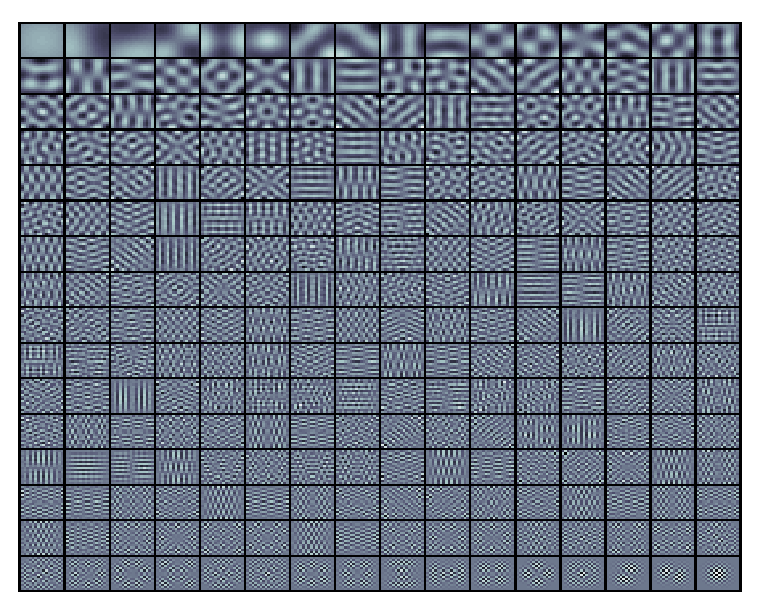
\includegraphics[width=0.45\textwidth]{./images/DL/DLstat/PCA_patchsize04.eps}
	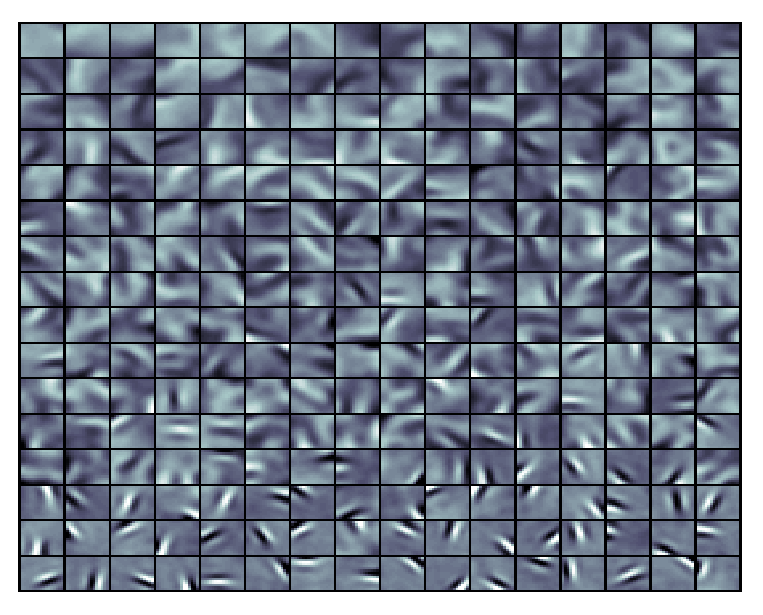
\includegraphics[width=0.45\textwidth]{./images/DL/DLstat/D_HR_lambda005.eps}
	\caption{\label{fig:PODvsDL} Dictionaries leaned by PCA and ODL from the set of HR patches of size $ \dimpsh = 16 \times 16 $. With ODL, only 256 atoms are chosen from 512 atoms.}
\end{figure}

Figure \ref{fig:PODvsDL} shows the adaptive dictionaries learned by PCA (left) and ODL (right) as ranked by their energy contents. The redundant dictionary by ODL has two times more atoms compared to PCA, which contains exactly $ \dimpsh = 16 \times 16 $ atoms as the dimension of the input patches. Only 256 over 512 atoms obtained by ODL are shown to be comparable with the PCA dictionary. The atoms are completely different in the two dictionaries. PCA dictionary has a sharp decline of variance content. Also, since the number of training patches is sufficiently large, the atoms look similar to discrete cosine transform (DCT) basis functions, which have modulated sine-wave patterns. The redundant dictionary from ODL contains more ``patterns'' for each level of scale, which is expected to be more adaptive to the data for sparse representation. 

Using a wavelet transform, there is no learning since the bases are predefined. The fields are decomposed into approximation and detail coefficients (horizontal, vertical and diagonal). The common Daubechies wavelet is used for its compact support and fast computation. The transform is performed on full fields. To test the sparsity effects, different thresholds are used. Detail coefficients larger than each threshold are retained while setting others to zeros, while approximation coefficients are kept unchanged. Inverse wavelet transform reconstructs the fields using these unchanged approximation and filtered detail coefficients. The sparsity is defined as the ratio of nonzero coefficients $ \dimtrunc $ (including both approximation and retained detail coefficients after filtering) and the dimension of the field $ \dimsh $. The NRMSE between reconstructed fields $ \hat{\z}_t $ and reference ones $ \z_t $ is estimated as in equation \ref{eq:NRMSE} to qualify the reconstruction for each level of sparsity $ (1- \dimtrunc/\dimsh )$.

With PCA, the dictionary $ \dict $ is learned from training patches $ \mathbf{P}_h $ extracted from all $ \left\lbrace \x_t \right\rbrace, t=1,...,\dimtl $. Its atoms  $ \left\lbrace \adicthigh{i} \right\rbrace $ are ranked by their variances $ \lambda_i $, i.e. $ \lambda_1 > \lambda_2 > ... > \lambda_{\dimsh} $. The dimensionality is reduced such that the retained information from only the first $ \dimtrunc $ principal components ($ \dimtrunc < \dimpsh $) is maximized. For a new field $ \z_t $, $ \mathbf{P}_h $ are extracted and projected onto the first $ \dimtrunc $ vectors:
\begin{equation}
	\adictco_i = \frac{\mathbf{P}_h \mydot  \adicthigh{i}}{\normtwo{\adicthigh{i}}} \:, i=1,2,...,\dimtrunc
	\label{eq:DL_efficiency3}	
\end{equation}
The filtered patches are estimated by combining the projected coefficients with the corresponding functions:
\begin{equation}
	\hat{\mathbf{P}}_h = \sum\limits_{i=1}^{\dimtrunc} {\adictco_i \adicthigh{i}}
	\label{eq:DL_efficiency4}
\end{equation}
Finally, the reconstructed field $ \hat{\z}_t $ is estimated by one-pixel overlapping as discussed in section \ref{subsec:patch_based_estimation}. The sparsity level is defined as $ 1-\dimtrunc/\dimpsh $, where the patch size at HR is $ \dimpsh = 16 \times 16 $. NRMSEs are estimated using equation \ref{eq:NRMSE}. 

KSVD and ODL learn $ \dict $ from $ \mathbf{P}_h $ \textit{a priori} with a high sparsity level ($ \lambda =0.2$, corresponding to about $ 15 $ non-zero coefficients). In the reconstruction step, all possible patches $ \mathbf{P}_h $ are extracted from each field $ \z_t $. The sparse code is estimated using LARS algorithm to solve:
\begin{equation}
	\dictco = \argmin_{\dictco} \left\lbrace \normtwo{\mathbf{P}_h - \dict \dictco_t} + \lambda \normone{\dictco} \right\rbrace
	\label{eq:DL_efficiency2}	
\end{equation}
The efficiency of the learned dictionary $ \dict $ is studied by varying $ \lambda $ in this step. For each $ \lambda $, $ \dictco $ is estimated and then used to re-estimate the patches $ \hat{\mathbf{P}}_h = \dict \dictco$ before reconstructing the global scene $ \hat{\z}_t $. Sparsity is measured as the average of $ 1- \normzero{\adictco_t}/\dimpsh $, where $ \adictco_t $ is the $ t- $th row of $ \dictco $. NRMSEs are estimated the same way as of wavelet transform or PCA.

\begin{figure}[t]
\centering
	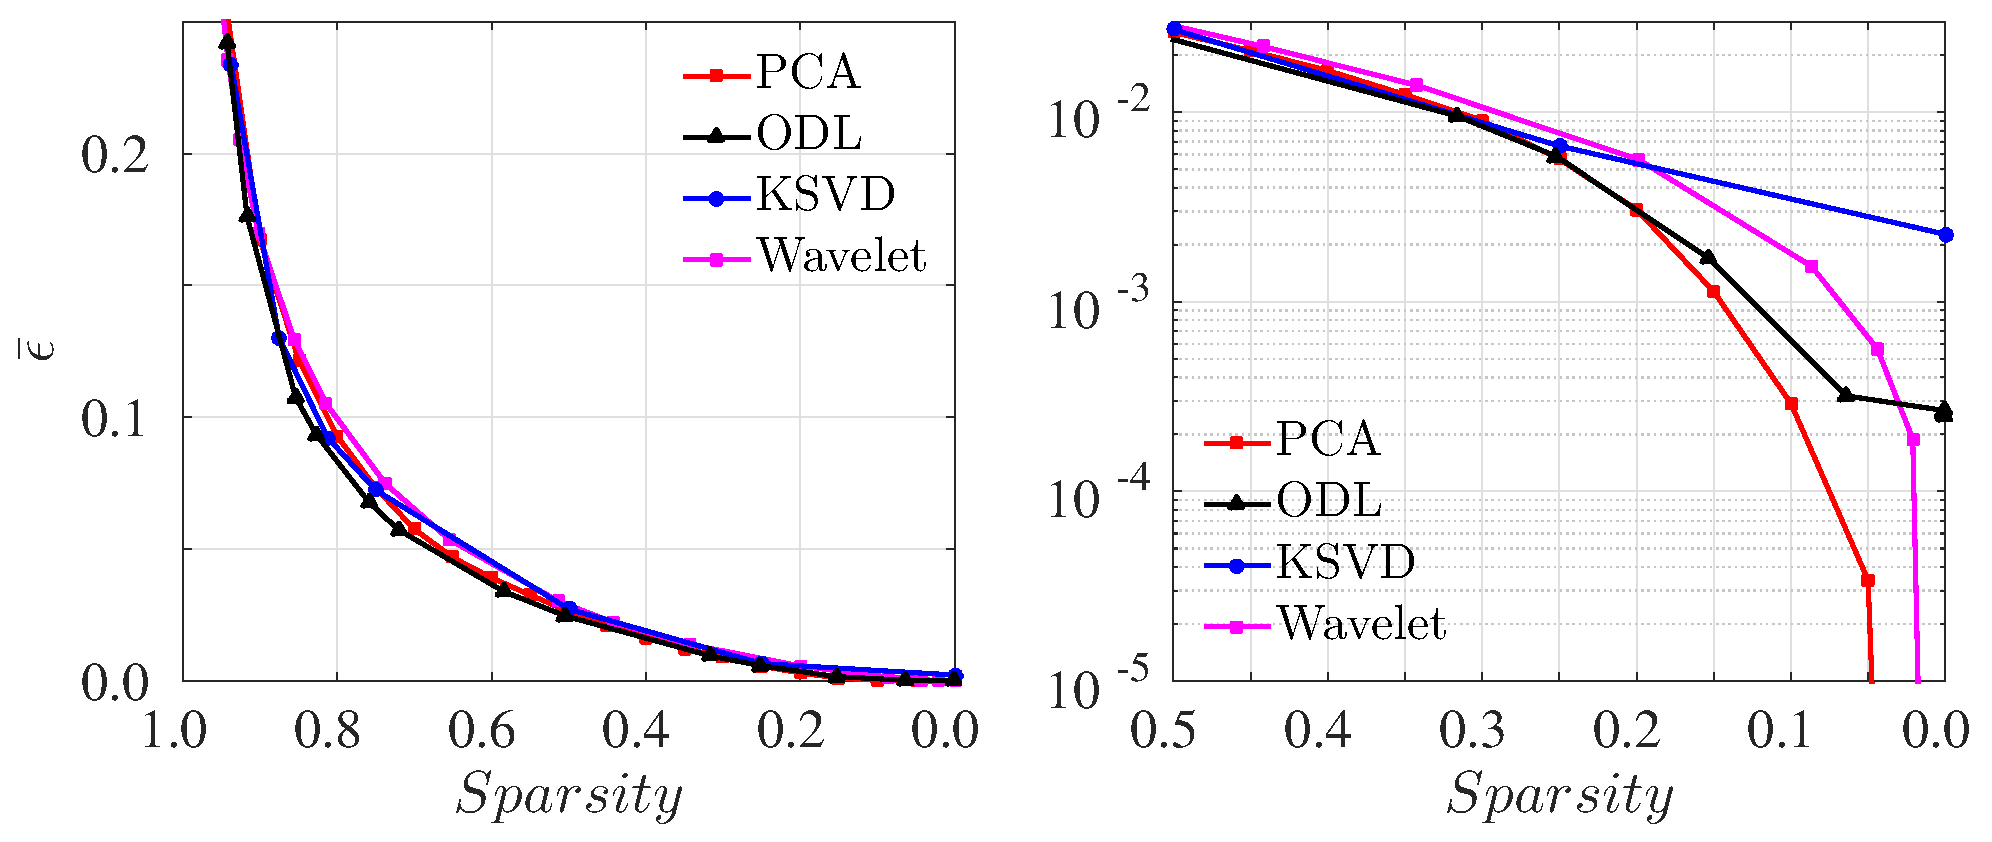
\includegraphics[width=\textwidth]{./images/DL/DLstat/Sparsity_vs_NRMSE_PCA_ODL_KSVD_WL_Dau_patchsize04.eps}
	\caption{\label{fig:Sparsity_vs_NRMSE} Sparsity vs error outside (left) and zoom in the region of low sparsity at semi-log scale (right) for different representations: wavelet (Daubechies), PCA, dictionary learning (ODL or KSVD). Wavelet transform is for the whole fields of size $ 96 \times 96$, while PCA and DL are for patches of size $ \dimpsh = 16 \times 16 $.}
\end{figure}

Figure \ref{fig:Sparsity_vs_NRMSE} shows the curves of NRMSE as functions of sparsity levels. These errors are estimated from five testing planes equally far from neighboring LTHS snapshots. All curves behave similarly as reducing the error when sparsity decreases. At high levels (larger than 0.5), there is a clear benefit of using DL. With the same number of non-zero coefficients, both ODL and KSVD give lower errors than PCA and wavelet transform. Few atoms from DL better represent the data than high variance principal components of PCA or predefined ones. Comparing the two DL methods, ODL is better than KSVD. When using more non-zero coefficients, errors by DL methods saturate at nonzero values. Since DL provides only an approximate solution. Wavelet transform and PCA give zero NRMSEs when using all coefficients because the transforms are exact.

The above comparisons demonstrate the advantages of representations using learned dictionaries over predefined ones. Comparing redundant and orthogonal representations, i.e. DL versus PCA, redundant dictionaries represent the fields more efficiently. They achieve the same level of error using less atoms. This suggests also that the sparsity and redundancy priors can be good candidates to help solving the ill-posed inverse problem of reconstructing HR fields from LR ones. Comparing the two common DL methods, ODL shows clear advantages both in term of efficient representation and computation effort and will be used in the rest of this chapter. 
 	
\subsection{Reconstruction of high resolution fields- subsampling cases}
To compare to other methods, LR fields are first subsampled from HR ones by a factor of $ 4 \times 4 $, i.e. $ \y_t = \Sub_s \z_t $, where $ \Sub_s: \R^\dimsh \mapsto \R^\dimsl $, $ \dimsh/\dimsl = 4 \times 4 $. Coupled LR and HR patches are extracted to train the dictionaries. Due to direct subsampling, the aliasing, which has not been addressed in previous works, will play an important role. This section investigates the ability of dictionary learning approaches to handle this aliasing problem.

\subsubsection*{Learning step}
\begin{figure}[t]
\centering
	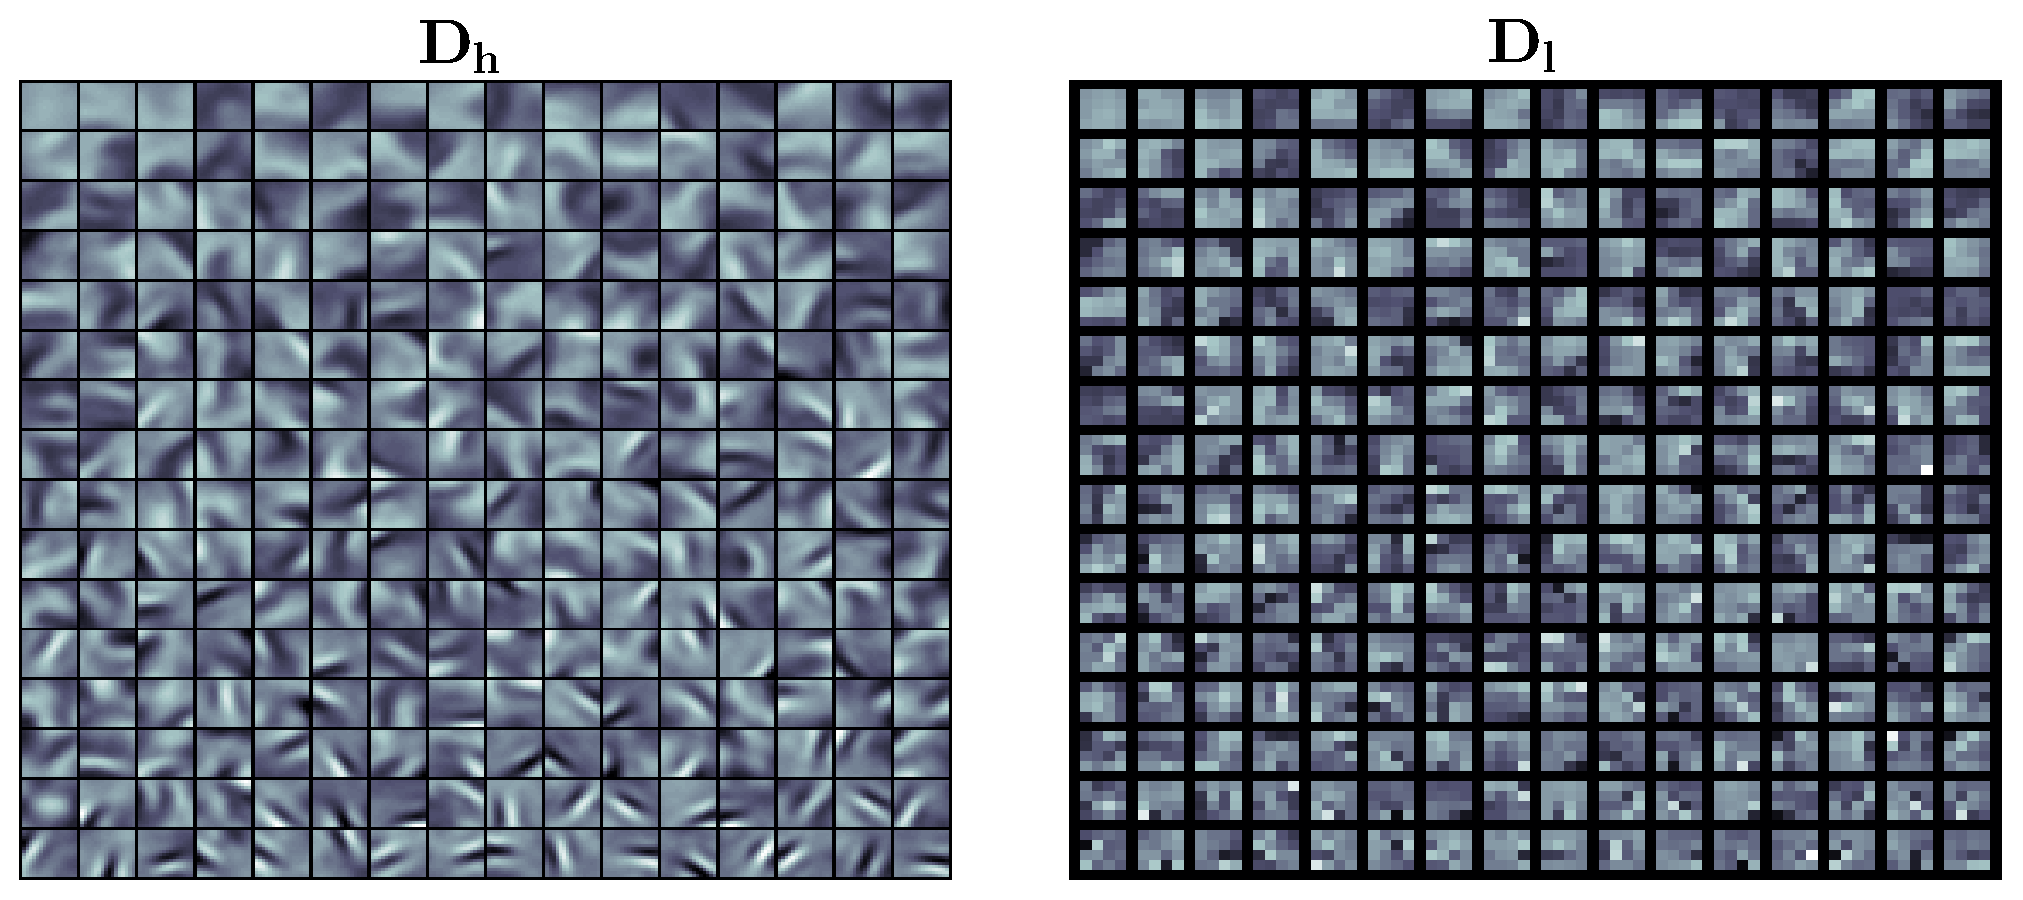
\includegraphics[width=\textwidth]{./images/DL/SR_sspacing04/subsampling/coupleddictionary_HRLR_lambda010.eps}
	\caption{\label{fig:D_HR_LR} Coupled dictionary of high and low resolution patches, with LR patches are of size $ 4\times 4 $, directly subsampled from their equivalent HR patches of size $ 16 \times 16 $. The regularization parameter $ \lambda $ for join learning are chosen such that about 16 non-zero coefficients are retained for reconstructing the joint patches of the training.}
\end{figure}

\begin{figure}[t]
\centering
	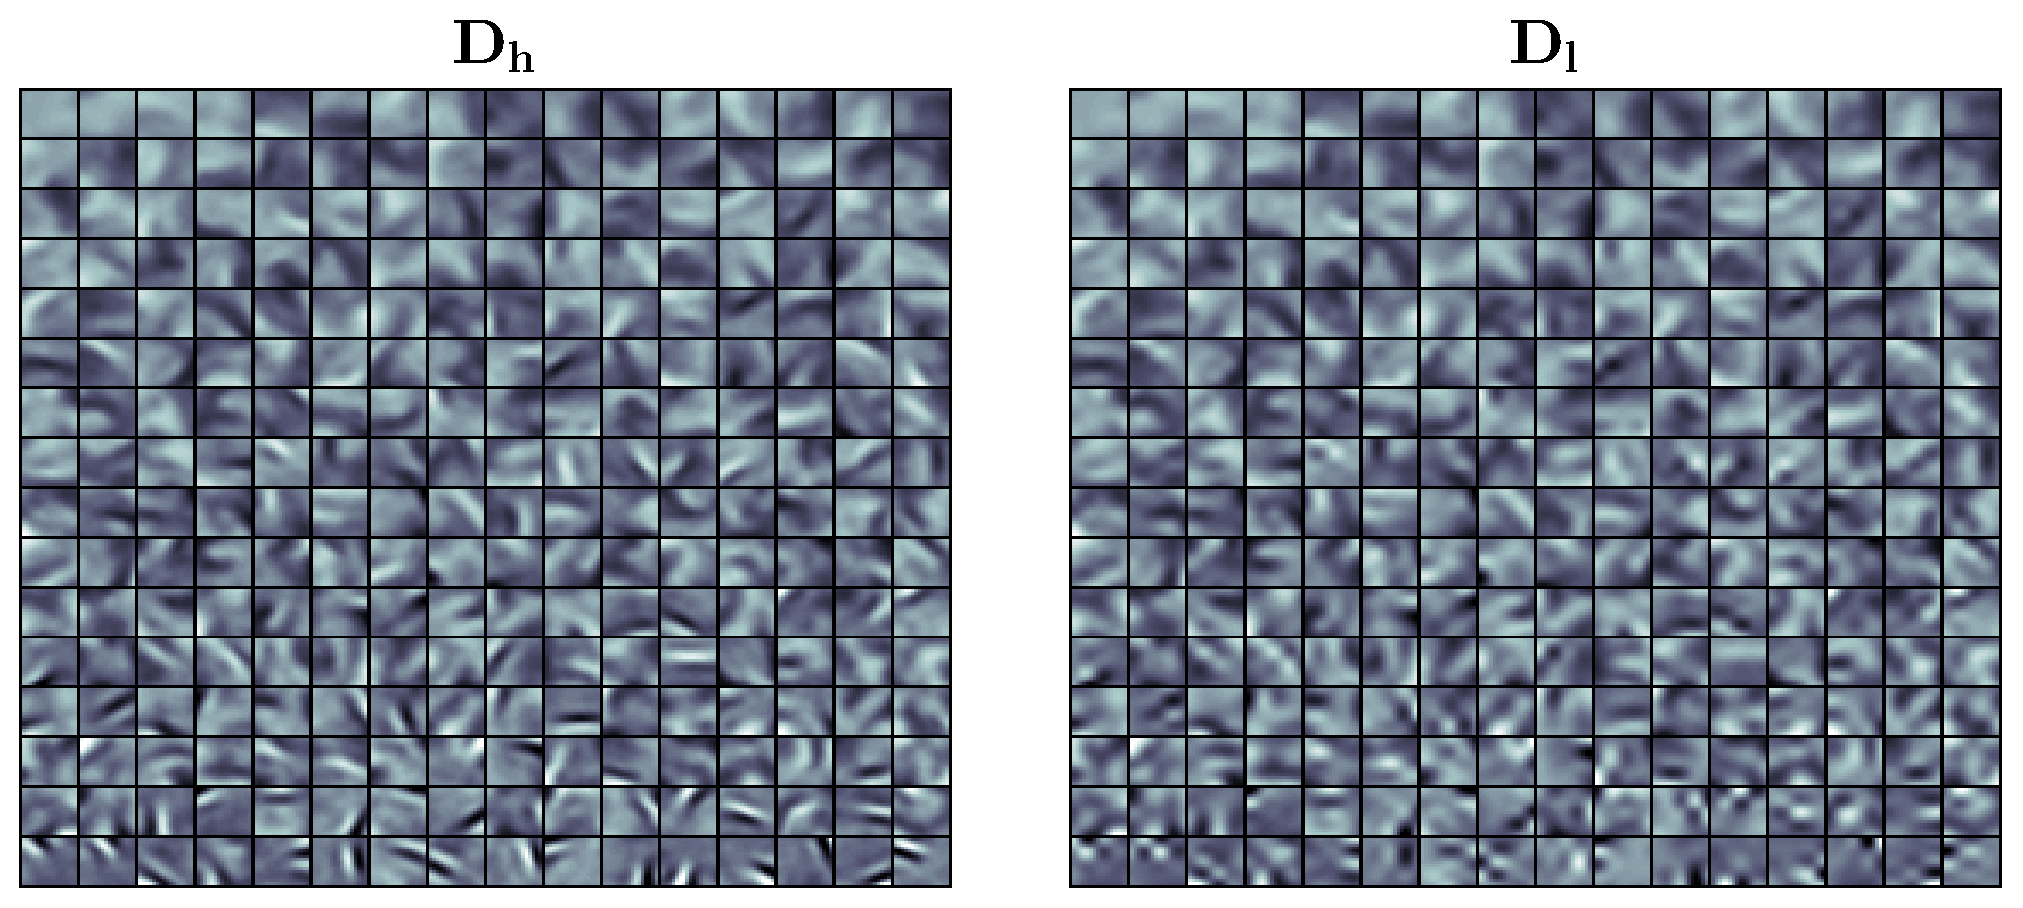
\includegraphics[width=\textwidth]{./images/DL/SR_sspacing04/subsampling/coupleddictionary_HRHRinterp_lambda010.eps}
	\caption{\label{fig:D_HR_HRinterp} Coupled dictionary of high and low resolution patches, where LR patches are of size $ 4\times 4 $, directly subsampled from their equivalent HR patches of size $ 16 \times 16 $. The regularization parameter $ \lambda $ for join learning are chosen such that about 16 non-zero coefficients are retained for reconstructing the joint patches of the training.}
\end{figure}

ODL \citep{mairal2010online} is used to learn a joint dictionary of HR and LR from the LTHS planes. The subsampling ratio in space is $ \dimsh/\dimsl = 4 \times 4 $, while the training samples are taken every $ \dimth/\dimtl = 6 $ snapshots in streamwise direction. From a total of $ 37 \times 16 $ training planes, small patches of size $ 4 \times 4 $ at LR are extracted via the extraction operator $ \extractlow{k} $, coupled with HR patches of size $ 16 \times 16 $ by $ \extracthigh{k} $. The choice of parameters is discussed in section \ref{subsec:DL_choice_params}.

Three approaches \textit{SR1}, \textit{SR2} and \textit{SR3} (table \ref{tab:DLapproaches}) are investigated. The interpolation step in \textit{SR2} plays only the role of transforming the field from LR to the same dimension as the HR one. The content should be rather the same, since the interpolation does not introduce any small-scale information. However, starting from the interpolated fields can bring the benefit of having a good large-scale information \textit{a priori}. The model will focus on small scales only. This approach have shown to be beneficial in many image processing problems.

Figure \ref{fig:D_HR_LR} shows dictionaries for HR and LR patches and figure \ref{fig:D_HR_HRinterp} shows dictionaries for HR and interpolated LR patches. In both figures, atoms are sorted according to their variances $ \normtwo{\adictco_i} $ when learning the dictionary (from the top-left). The most significant atoms contain mostly large scales, while less significant ones represent high-frequency contents. Coupled atoms show similar patterns. The relation between LR and HR patches are now encoded in the relation between LR and HR dictionaries. The assumption of coupled representations in this case also implies that LR atoms are approximately subsampled from the HR ones as shown in equation \ref{eq:DL_approach5}. 

\subsubsection*{Reconstruction step}
Having learned dictionaries $ \{\dicthigh,\dictlow \} $ at hand, from given $ \y^\ext $ different from the training data, the HR field $ \z^\ext $ is reconstructed by using algorithm \ref{algo_SR}. $ \y^\ext $ is also assumed to be directly subsampled from $ \z^\ext $ the same way as in the training data, i.e. $ \y^\ext = \Sub_s \z^\ext $. From $ \y^\ext $, all LR patches $ \mathbf{P}_l^\ext $ with one-pixel overlapping are extracted. The sparse code is estimated by solving the optimization problem in equation \ref{eq:algo_SR_4}. $ \dictco^\ext $ is then used to reconstruct HR patches as $ \hat{\mathbf{P}}_h^\ext = \dicthigh \dictco^\ext $ and put back into the global scene of $ \hat{\z}^\ext $. 

LR and HR patches of sizes $ \dimpsl = 4 \times 4 $ and $ \dimpsh = 16 \times 16$ respectively are extracted from all training planes. The sparse code $ \dictco^\ext $ is estimated from LR patches. Each row has at most $ \normzero{\dictco^\ext} = \dimpsl = 16 $ nonzero coefficients. It means that HR patches are reconstructed from maximum $ 16 $ atoms within $ \dicthigh $, a strong constraint on the reconstruction accuracy (see figure \ref{fig:Sparsity_vs_NRMSE}). The nature of the data also affects the accuracy in the sense how good is the Sparse-Land prior. Also, this constraint addresses the problem of designing more efficient representations of the data to reduce the error when using the same number of atoms. 

Using all three approaches presented in table \ref{tab:DLapproaches}, the models can reconstruct the fields in the same accuracy as the spline interpolation but not better. This is due to the severe situation where the presence of aliasing makes equation \ref{eq:DL_approach5} a very crude assumption. The subsampling of a small atoms brings a very strong aliasing effect that coupled dictionaries could not efficiently handle. The next section will study the capability of the present approach when the aliasing problem is absent from the LR data.

\subsection{Reconstruction of high resolution fields- the downsampling case}
\begin{figure}
	\centering
	
\includegraphics[width=0.6\textwidth]{./images/DL/SR_sspacing04/downsampling/dictionary_couplefeatures_patchesHR.eps}
	\caption{Dictionary of the residual between HR and interpolated LR.}
	\label{fig:SR_dictionary_residual}
\end{figure}

This section investigates the possibility of the current approach to estimate the HR fields given the LR ones in the case of downsampling, i.e. with anti-aliasing prefiltering:
\begin{equation}
\y_t = \Sub_s \LPF_s \z_t
\end{equation}
where $ \Sub_s $ and $ \LPF_s $ are the spatial subsampling and low pass filter respectively. Bicubic filter in Matlab built-in function \textit{imresize} is used for the prefiltering and interpolation step. It was shown also in section \ref{sec:chap3_theapproach} that the assumptions Sparse-Land model at HR also lead to the relation $ \mathbf{P}_\ell =  \Sub_s^\ext \LPF_s^\ext \mathbf{P}_h$ between LR and HR dictionaries. $ \Sub_s^\ext $ and $ \LPF_s^\ext $ are local versions of $ \Sub_s $ and $ \LPF_s $ applying to patches. 

We compare the three methods of coupled dictionary learning, the so-called \textit{SR1}, \textit{SR2} or \textit{SR3}, presented in table \ref{tab:DLapproaches}. To recall \textit{SR1} and \textit{SR2} couple either LR or interpolated LR patches with HR ones, while \textit{SR3} couples the residuals with the features of derivatives. The procedure follows the previous section of subsampled fields, with learning parameters in table \ref{tab:DLparams}. HR patches $ \mathbf{P}_h$ are extracted from LTHS fields and coupled with LR patches $ \mathbf{P}_\ell$. The dictionaries are trained \textit{offline} from $ \{\mathbf{P}_h, \mathbf{P}_\ell\}$, and used in \textit{online} reconstruction stage for all HTLS measurements to reconstruct HTHS fields. 

We use three quantities for comparisons: the average NRMSE between reconstructed and reference velocity fields estimated using equation \ref{eq:NRMSE}, the 2D energy spectra of the velocity fields and of the errors. These three quantities give a complete view to qualify different approaches. Only the most difficult planes, which are equally far from LTHS measurements, are used to estimate the errors. Error estimated using these planes will better represent the generalization capability of the approaches.

\begin{figure}
	\centering
	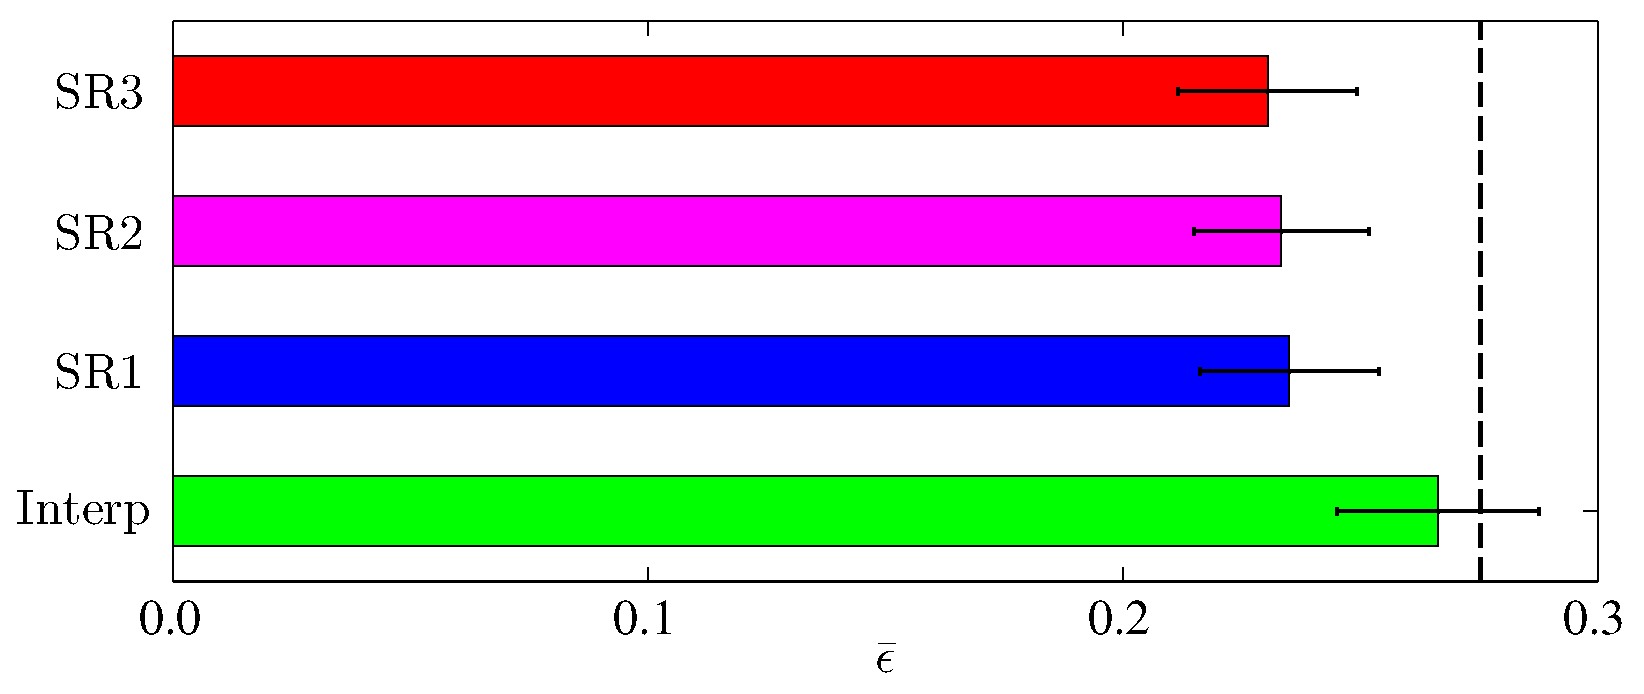
\includegraphics[width=0.9\textwidth]{./images/DL/SR_sspacing04/downsampling/NRMSE_compare_all_spacespacing_04.eps}
	\caption{Means and standard deviations of NRMSEs estimated between reference and reconstructed fields of all middle planes (at the center of blocks bounded by the two LTHS planes). The reconstructions are by spline interpolation and super-resolution using three different methods:: \textit{SR1}, \textit{SR2} and \textit{SR3} (see table \ref{tab:DLapproaches}). NRMSEs are $ 0.267 \pm 0.021 $, $ 0.235 \pm 0.019 $, $ 0.233 \pm 0.018 $ and $ 0.230 \pm 0.019 $ respectively. The NRSME of spline interpolation in the equivalent subsampling case is 0.276 (dashed black line).}
	\label{fig:NRMSE_compare_all_spacespacing_04}
\end{figure}

Figure \ref{fig:NRMSE_compare_all_spacespacing_04} shows the average NRMSEs of different reconstructions, either interpolation or reconstruction by coupled dictionaries using \textit{SR1}, \textit{SR2} or \textit{SR3} approaches. The three DL models reduce NRMSEs by $ 11.99 \% $, $ 12.73 \% $ and $ 13.86 \% $ respectively compared to the simple interpolation. \textit{SR3} gives the most accurate reconstructions by coupling the residuals, essentially contain only small scales, with derivatives of large-scale structures.

\begin{figure}
	\centering
	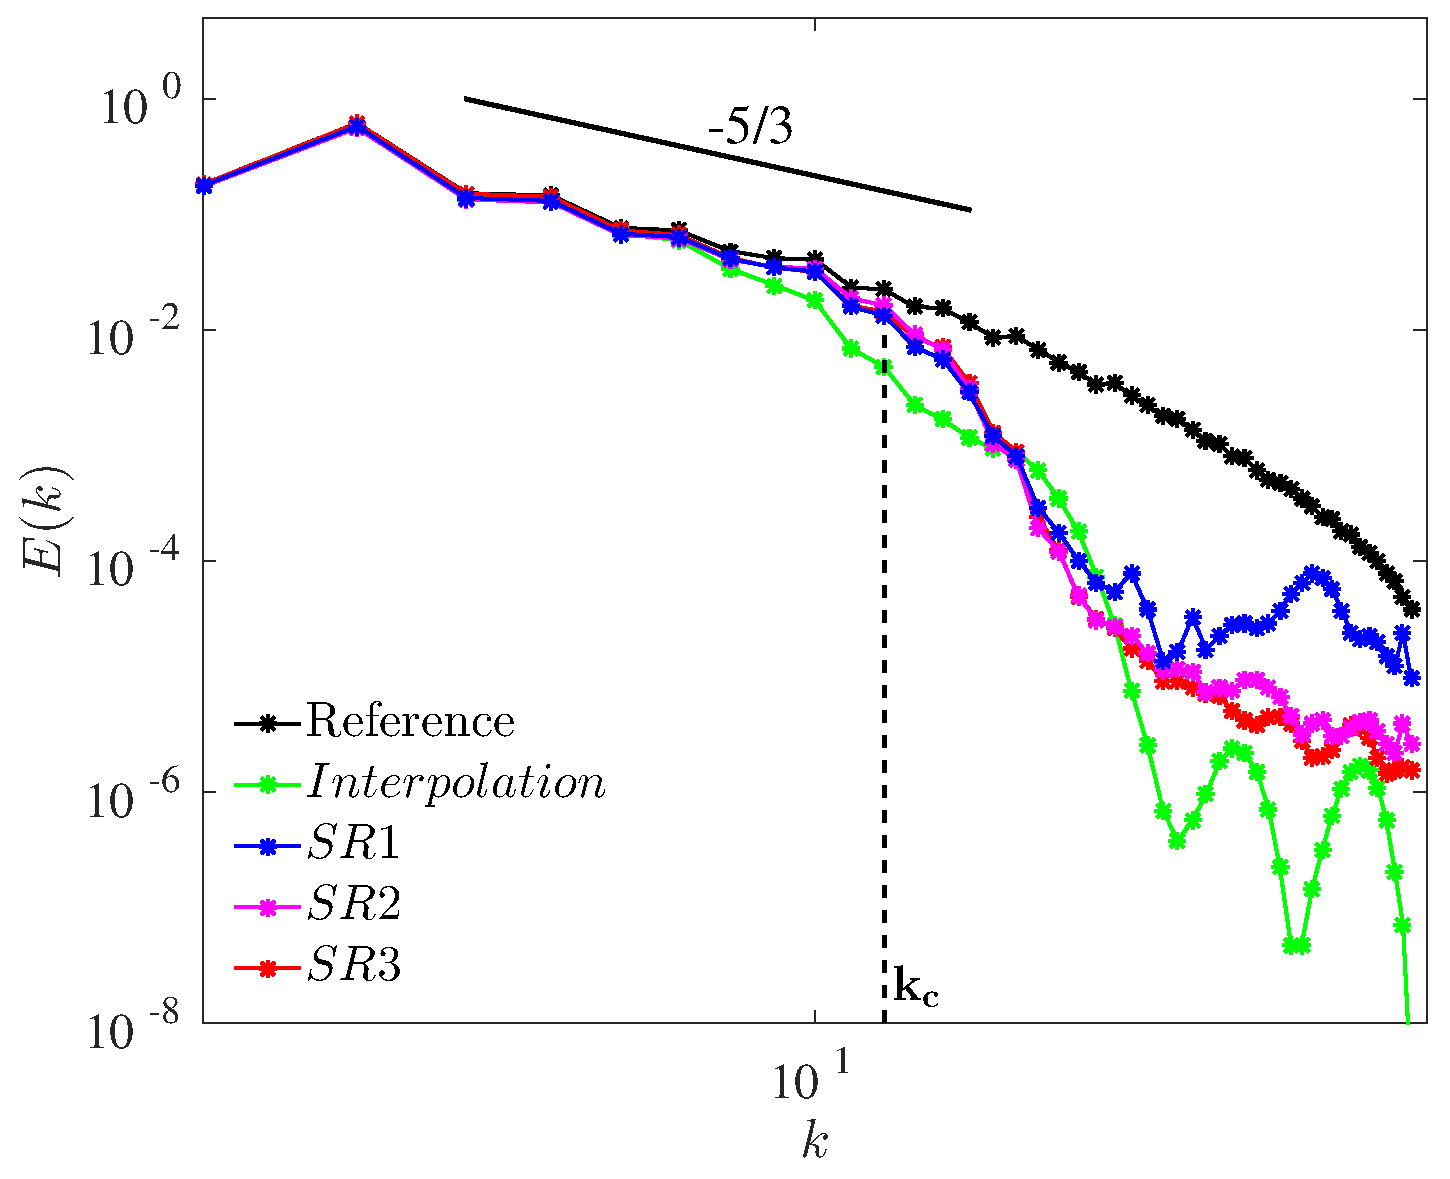
\includegraphics[width=0.75\textwidth]{./images/DL/SR_sspacing04/downsampling/spectra2d_spacespacing_04.eps}
	\caption{2D spectra of all planes used to computed the NRMSEs in figure \ref{fig:NRMSE_compare_all_spacespacing_04}, from reference, interpolation and SR by three different methods: \textit{SR1}, \textit{SR2} and \textit{SR3} (see table \ref{tab:DLapproaches}). For scales from $ 0.5k_c $ to $ 1.5 k_c$, energy losses of SR fields compared to reference ones is $ 24\% $, $ 22\% $ and $ 21\% $ respectively, while that of interpolation is $85 \% $.}
	\label{fig:spectra2d_spacespacing_04}
\end{figure}

To further understand the quality of the reconstructed fields at different scales, figure \ref{fig:spectra2d_spacespacing_04} shows the 2D spectra of reference fields and different reconstructed ones. All methods capture good large scales till about $ 0.5 k_c $, where $ k_c $ is the cutoff wave number defined by the subsampling ratio. The interpolation, starting from the downsampled fields with prefiltering step to avoid aliasing, loses already energy at large scales and capture almost no small scales. By coupling the dictionaries, the reconstructed fields recover the large-scale information with some small scales. If considering only the scales between $ 0.5k_c $ and $ 1.5k_c $, the energy loss of interpolated fields is $ 85\% $, while those are $ 24\% $, $ 22\% $ and $ 21\% $  for \textit{SR1}, \textit{SR2} and \textit{SR3} respectively. The benefit of SR is significant in this most interesting range of scales. Larger than $ 1.5k_c $, all reconstructions are not reliable. Smaller than $ 0.5 k_c $, spectra of all reconstructed fields are already very accurate. 

\begin{figure}
	\centering
	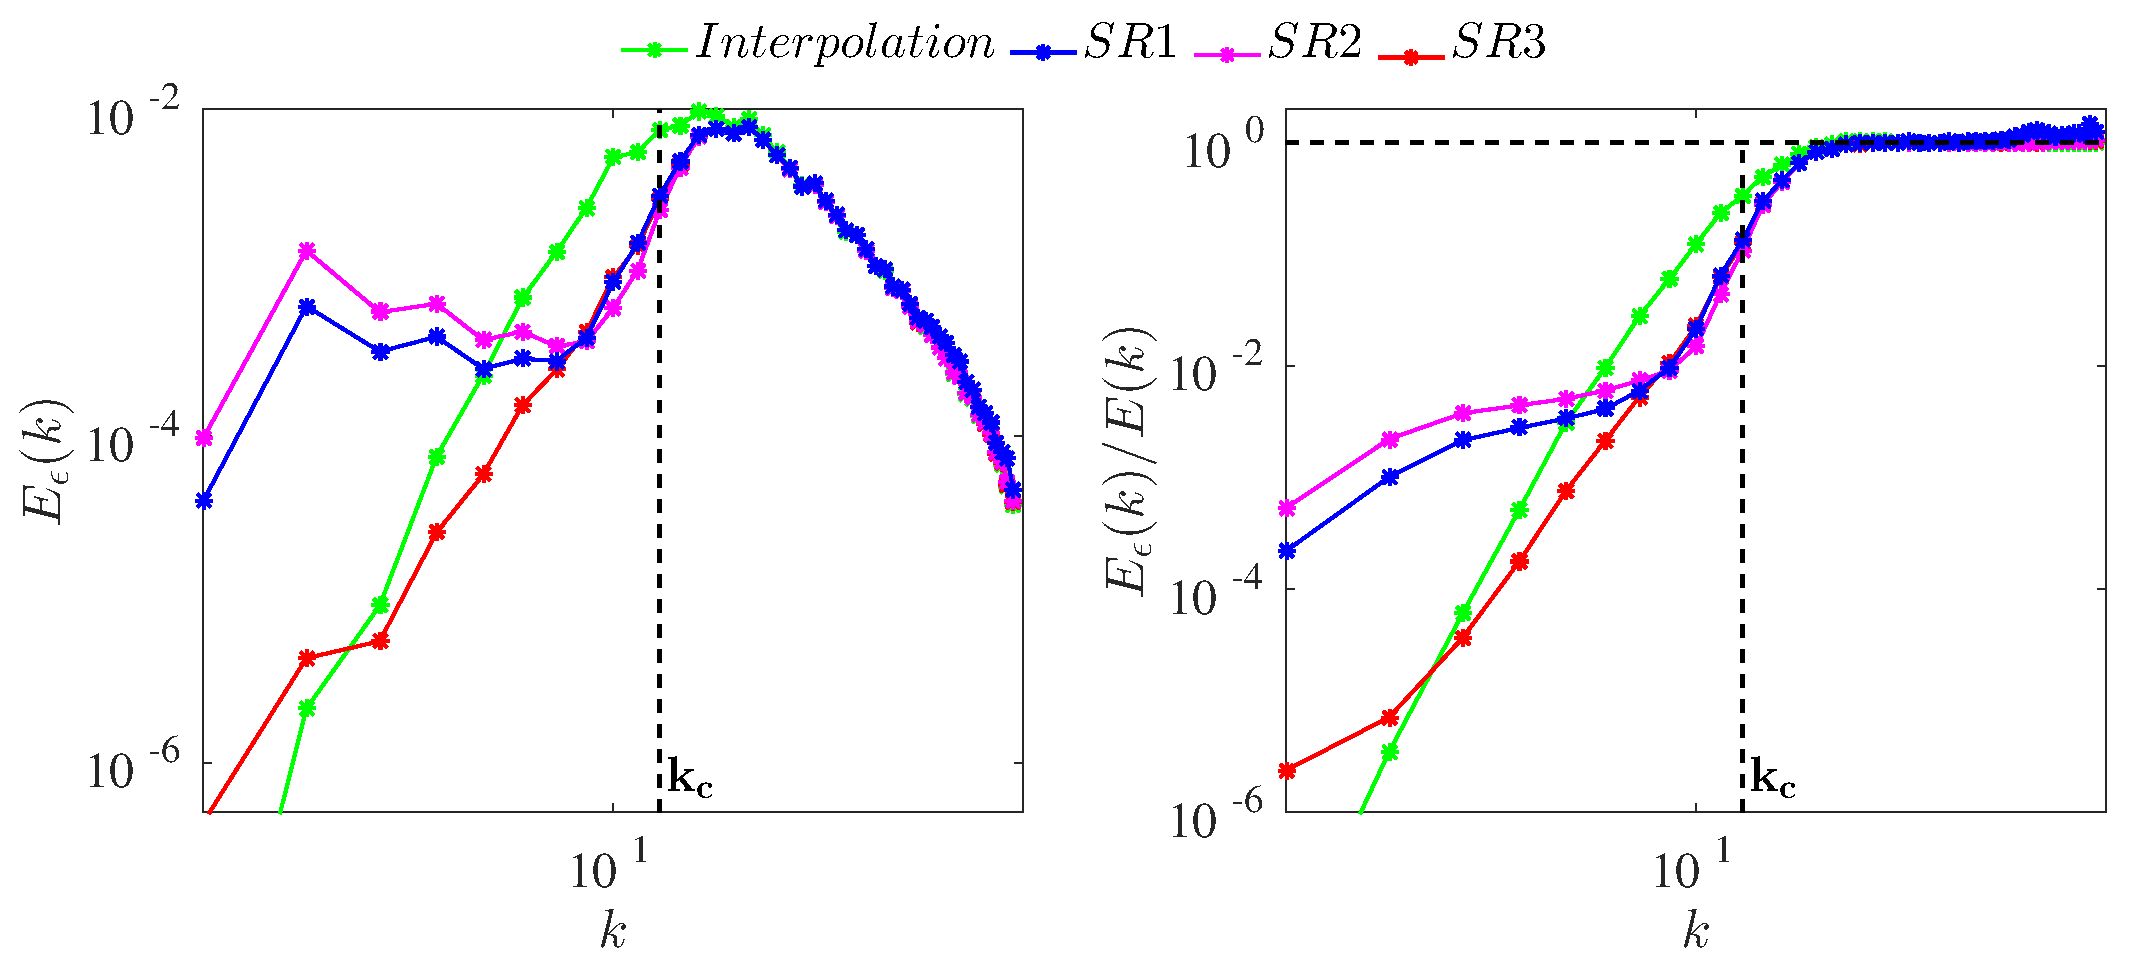
\includegraphics[width=\textwidth]{./images/DL/SR_sspacing04/downsampling/errspectra2d_nonnormalized_normalized_timespacing_06_spacespacing_04.eps}
	\caption{(Left) 2D spectra of errors, which are the different between the reference and reconstruction by interpolation and three different SR methods as described in \ref{sec:joint_learning_methods}. (Right) 2D spectra of errors normalized by the energy spectrum of the reference (the black curve in figure \ref{fig:spectra2d_spacespacing_04}).}
	\label{fig:errspectra2d_nonnormalized_normalized_timespacing_06_spacespacing_04}
\end{figure}

Figure \ref{fig:errspectra2d_nonnormalized_normalized_timespacing_06_spacespacing_04} (left) shows the spectra of the errors, which are the differences between the reference and reconstructed fields by all methods. Errors are very low at small wave numbers, reach a maximum around $ k_c $ and reduce at higher wave numbers. Integrals of these curves give the mean-square errors of each reconstruction method. To better qualify the error at each scale, the curves are normalized by the energy spectrum of the reference (the black curve in Figure \ref{fig:spectra2d_spacespacing_04}). The normalized spectra of errors are interpreted as the percentage of error at each scale. The interpolation gives very small relative errors at large scales, but grow rapidly near $ k_c $. Error spectra of all SR methods collapse at $ 0.5k_c $ and reach a maximum of $ 100 \% $ error at around $ 1.5k_c $. Smaller than $ 0.5k_c $, \textit{SR1} and \textit{SR2} gives slightly higher errors compared to \textit{SR3}. \textit{SR3} is more accurate since it starts from the interpolated large scales, while those information are re-estimated by \textit{SR1} and \textit{SR2}. Also, \textit{SR3} focuses more on the missing information of small scales by using derivatives as features and following the patterns of larger ones. 

From the above comparisons, coupled dictionary approaches demonstrate clear benefits compared to the simple interpolation, with errors reduced by about $ 15\% $. From the energy spectra or spectra of errors, the benefits mostly come from the range of scales between $ 0.5k_c $ and $ 1.5k_c $, where $ k_c $ is the cutoff defined by the grid of LR measurements. The loss of energy in this range is reduced from $ 80\% $ with interpolation to $ 20\% $ by DL approaches. The spectra of the errors also show that most of benefits come from this range of scales, before reaching $ 100\% $ at around $ 1.5k_c $.

\section{Concluding remarks}
This chapter has discussed the possibilities of applying dictionary learning, a successful approach in the field of signal and image processing, to turbulence studies. The method finds a representation for the data by generalizing principal component analysis to sparse representation in a redundant dictionary. \textit{Redundancy} means that the number of atoms can be larger than the dimension of input vectors, ignoring the orthogonality constraint of PCA. This implies the \textit{sparsity}, i.e. the representation is composed by a linear combination of only a few atoms. These properties make the learned dictionary a more adaptive representation of the data. Sparsity can also play the role of a prior about the system when solving the inverse problem of HR field reconstruction. 

To investigate the efficiency of DL in representing the data, the learned dictionaries by this approach have been compared against PCA and predefined wavelet dictionaries. Reconstruction errors as functions of sparsity, i.e. the number of atoms used, are shown as the measure of efficiency. Adaptive dictionaries show some superiority compared to the predefined ones. The benefits are mainly from the high sparsity levels, when less than half the number of coefficients are non-zero. 

DL is then used to reconstruct HR velocity fields from LR measurements. The approach is called \textit{coupled dictionary learning}, inspired from the single image super-resolution application \citet{yang2010image,zeyde2012single}. By learning coupled representations of LR and HR fields from the data, a nonlinear relation is established and generalized to perform the reconstruction task. With the same idea, different preprocessing techniques are tested. The coupling can be between HR and LR fields or their interpolation. Another approach focuses more on the small-scale information by coupling the small scales with the derivatives of interpolated fields. 

The first attempt is for the configuration where LR fields are directly subsampled from HR ones without any anti-aliasing prefiltering step. This is \textit{a priori} not a favorable case due to the presence of aliasing terms. However, it is worth studying since this setup mimics what would happen in a real experiment. It is interesting also to see how well learned dictionaries can handle aliasing. Results show that DL is inoperative to recover some small scales on top of the interpolated large-scale information. 

To understand whether the failure comes from the approach or from the aliasing, another case is investigated where LR fields are downsampled from the HR ones with a prefiltering step. The same approach with  identical parameters is used. Results show significant improvements of reconstruction accuracy, with about $ 15 \% $ reduction of NRMSEs compared to interpolation. Spectral analyses also show that most benefits are at the frequency range of $ 0.5 k_c$ to $ 1.5k_c $, where $ k_c $ is the cutoff wave number corresponding to the downsampling ratio. In term of energy, simple interpolation loses $ 85 \% $ in this range scales, while this loss is reduced to about $ 20 \% $ with DL approaches.

The above results demonstrate the capability and limitations of DL approaches in solving the reconstruction problem in turbulence. The corresponding prior, which is the duality between sparsity and redundancy, is robust. The first attempt has not succeeded to reconstruct HR fields from direct subsampled LR ones due to the aliasing problem. This attempt addresses also the question on designing a good sensing system or post-processing techniques to deal with aliasing terms if exist.

This chapter has presented a similar configuration as regression models to learn the mapping function between large and small scales. However, the learning is localized thanks to the patch-wise approach. This property of dictionary learning approach can be beneficial when applying to other configurations where the training and testing samples are of different scenes. For example, the training HR fields could be a small region of the whole field, while LR one can be larger. In such case, dictionary approach is the only candidate among all methods presented in this thesis. 



\chapter{Non-local similarity-based propagation model} 
\label{chap_NLM} 

This chapter proposes a novel model that combines low-resolution measurements in space and time in order to reconstruct fully resolved turbulent fields. This method tackles the problem of fusing high-time-low-space and low-time-high-space resolution measurements mentioned in section \ref{sec:probdef2}. The model exploits local structures in large scale measurements to reconstruct small scales. The idea is to assume that small scales are essentially advected by large scales. This is based on the scale similarity hypothesis, where information at adjacent ranges of scales are strongly correlated. The model is further developed from the non-local means (NLM) denoising filter \citep{buades2005review}, which is very simple but efficient, and widely used in image processing.

The proposed model is applied to the streamwise velocity fields from DNS data of isotropic turbulence as described in section \ref{sec:data_isotropic}. Due to the absence of time resolved fields, \textit{the streamwise direction is associated to the time dimension}, while the other two spatial directions are the spanwise and the vertical ones. Within this chapter, parameters of the model will be optimized. Model performances are also investigated by fixing one subsampling ratio in either space or time (spanwise) while varying the other. Detailed analysis of model performances are presented, but further comparisons with other methods will be investigated in chapter \ref{chap_comparisons}.

\section{Non-local means}
Non-local means (NLM) was originally proposed by \citet{buades2005review} to deal with the single image denoising problem. It has been then extended to solve other inverse problems of image reconstruction such as inpainting (to fill in missing pixels) or super-resolution (to increase image resolution). The model assumes that image content is likely to repeat in many regions. The estimate of each pixel is a weighted average of its neighbors assigned with different weights. These weights are estimated as the similarity of the denoised/inpainted/super-resolved pixel with its neighbors. By proposing several estimates of a single pixel, NLM yields redundancy by using several observations of similar scenes obtained from different locations within the same image. These multiple observations of underlying ground truth help in solving the ill-posed inverse problem.

\subsection{Non-local means filter for denoising}
\begin{figure}
	\centering
	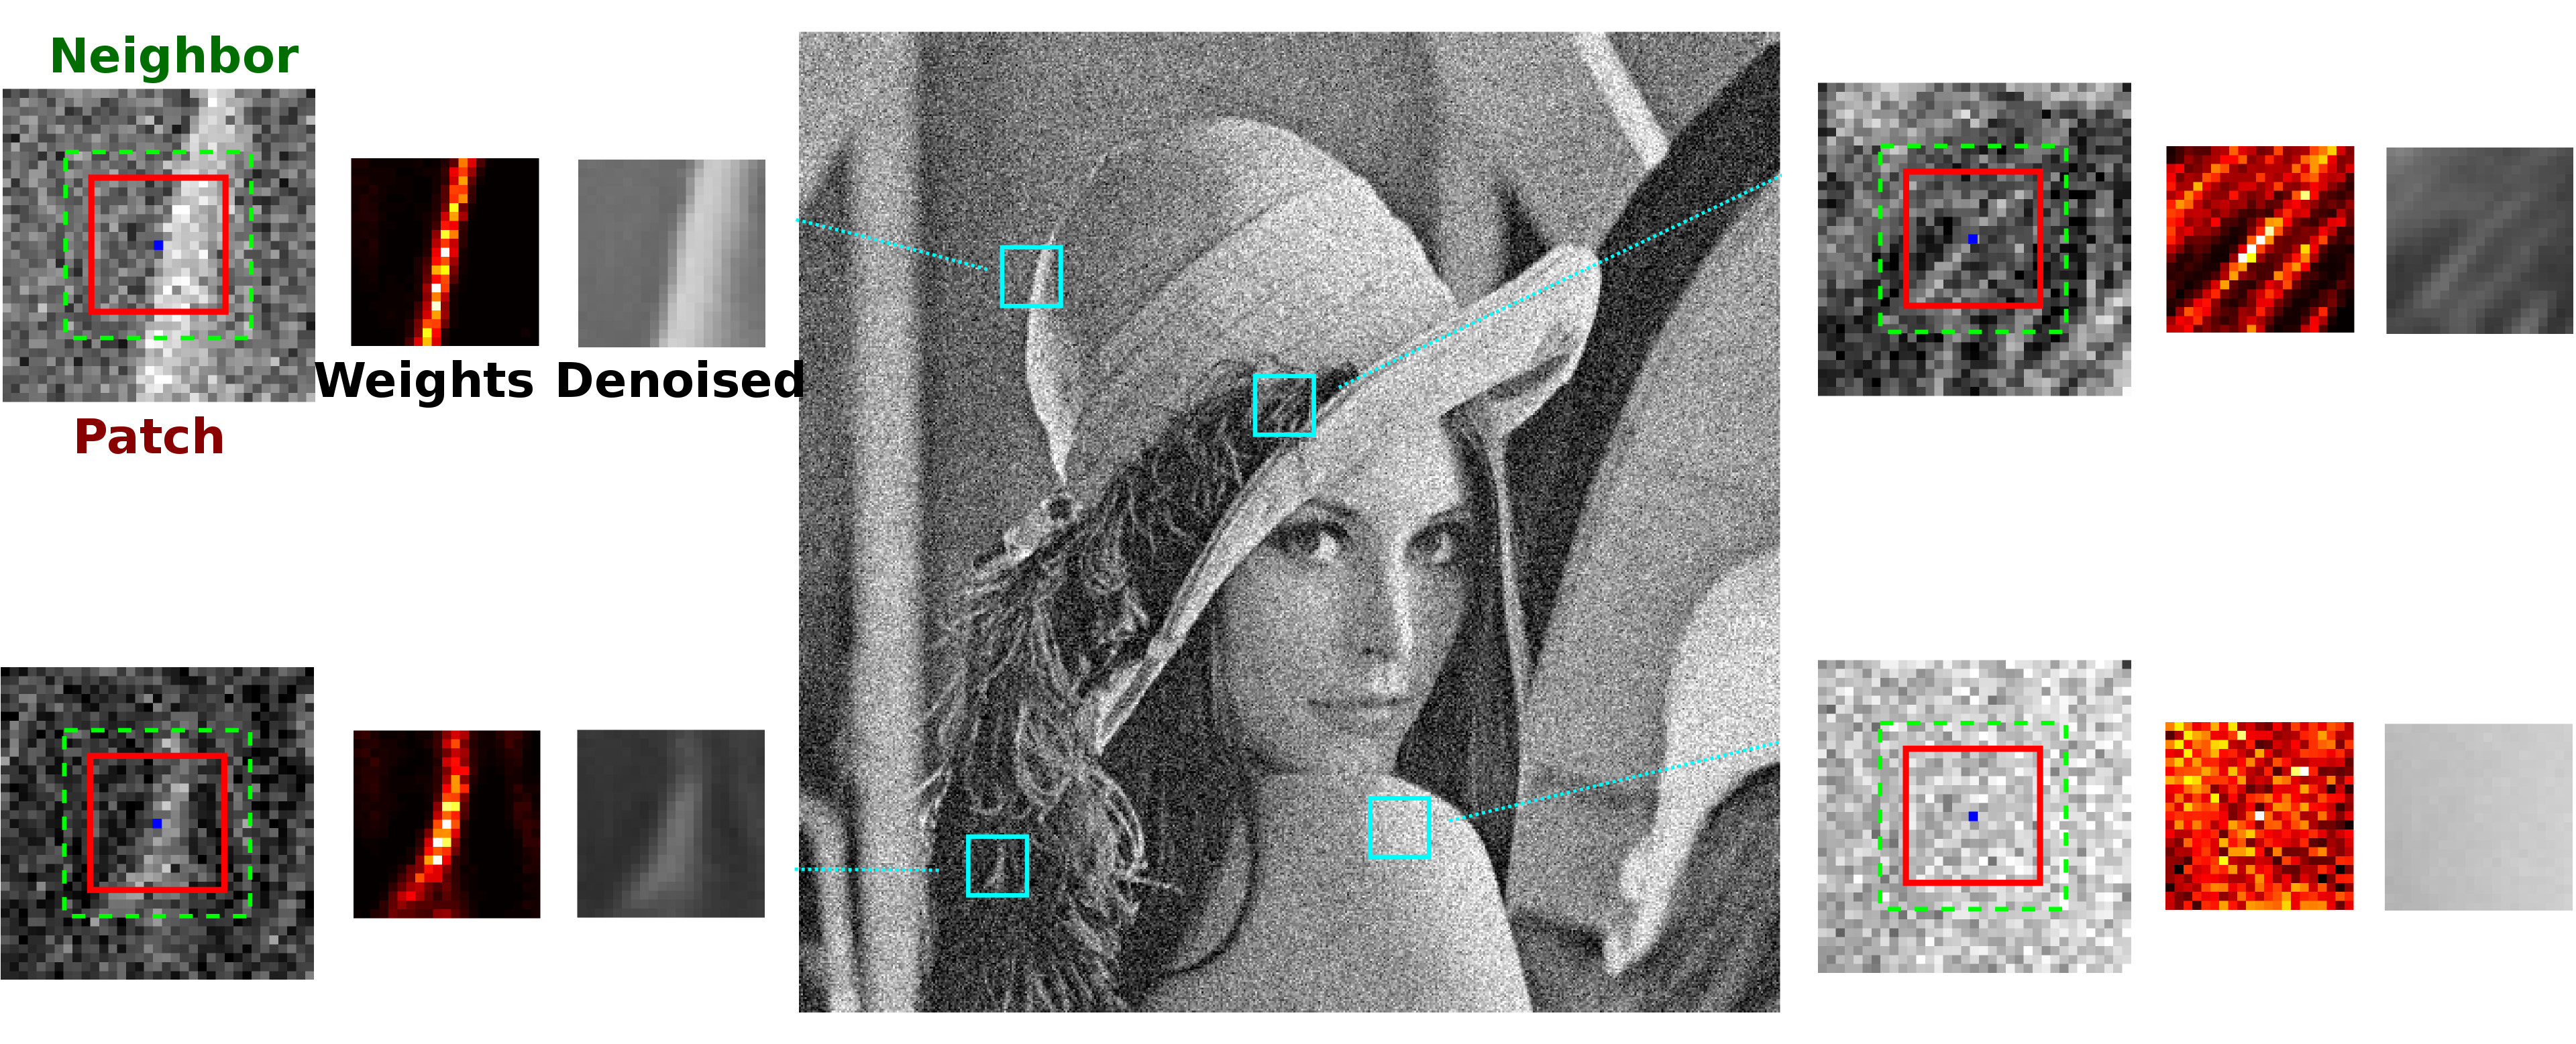
\includegraphics[width=\columnwidth]{./images/NLM/lena.png}		
	\caption{\label{fig:lena} Image denoising using non-local means. Four sample patches in red extracted from noisy image and centered at blue dots. The estimate of each point are weighted average of its neighbors, and weights are computed as the similarity of the moving patches compared to the reference patch. Photo credit: \citet{foi2016foveated}.}
\end{figure}

The NLM denoising filter is simple but rather robust. Figure \ref{fig:lena} illustrates how the NLM filter works on a sample image. Denoting $ \mybold{z}_t \in \R^{\dimsh} $ as the column vector of a 2D noisy image, the NLM filter denoises the $ k- $th pixel as a weighted average of its neighboring noisy pixels:
\begin{equation}
	\hat{\mybold{z}}_t[k]=\frac{\displaystyle \sum_{i\in\neighbor_k}w[k,i]\mybold{z}_t[i]}{\displaystyle \sum_{i\in\neighbor_k}w[k,i]}
\end{equation}
$ \neighbor_k $ is the set of neighboring pixels of the $ k- $th pixel. The local weight coefficient $ w[k,i] $ is the similarity between the $ k- $th and $ i- $th pixels:
\begin{equation}
	w[k,i] = \myexp{ -\frac{\|\mathcal{R}_s^k\mybold{z}_t-\mathcal{R}_s^i\mybold{z}_t\|^2_2}{2\nlmfilparam^2}}
\end{equation}
where the operator $ \mathcal{R}_s^k: \R^{\dimsh} \mymapto \R^\dimpsh$ extracts 2D patches of size $ \sqrt{\dimpsh}\times \sqrt{\dimpsh} $ centered at the $ k- $th pixel. These patches are then arranged in a column vector in lexicographical order. When $ \dimpsh=1 $, the NLM filter becomes a bilateral one. The global filter parameter $ \sigma $ regulates the decay of the exponential expression. It controls the contribution of the $ i- $th pixel on the estimation of the $ k- $th pixel. Geometrical priority can also be introduced, where high weights are given to closer neighbors than further ones.


\subsection{Generalized non-local means for super-resolution}
The idea of the NLM filter has been generalized to perform video super-resolution \citep{protter2009generalizing} by introducing time dimension. The aim is to estimate HR sequence of images $ \mybold{z}_t \in \R^{\dimsh}, t=1,2,...,\dimth , $ from corresponding LR sequence of images $ \mybold{y}_t \in \R^{\dimsl}$ ($ \dimsl <\dimsh $). NLM exploits the self-similarity property of natural images in the sequence. The model assumes that common scenes are shared by many snapshots in the sequence. Derivation and mathematical explanation can be found in \citet{protter2009generalizing}. The closed form solution is simplified, where each HR pixel is estimated as a weighted average of neighboring LR pixel in a space-time window:
\begin{equation}
	\hat{\mybold{z}}_{t_\knot}[k]=\cfrac{\displaystyle \sum_{t\in\neighbor_{t_\knot}}\sum_{i\in\neighbor_k}w[k,i,t]\mybold{y}_t[i]}{\displaystyle \sum_{t\in\neighbor_{t_\knot}}\sum_{i\in\neighbor_k}w[k,i,t]}
\end{equation}
where $ \neighbor_{t_\knot} $ is the set of neighboring snapshots in time of the $ t_\knot$-th one. The weight $ w[k,i,t] $, defined as the probability of the $ k- $th HR pixel estimation coming from the $ i $-th LR pixel, is estimated as:
\begin{equation}
	w[k,i,t] = \myexp{ -\frac{\normtwo{\mathcal{R}_s^k\mybold{y}_{t_\knot}-\mathcal{R}_s^i\mybold{y}_t}}{2\nlmfilparam^2}}
\end{equation}
This solution exits when there is at least one non-zero weight $ w[k,i,t] $.

It is natural to test this idea to reconstruct HTHS turbulent fields $ \Z $ of size $ \dimth \times \dimsh $ from the corresponding HTLS measurements $ \Y $ of size $ \dimth \times \dimsl $ ($ \dimsl < \dimsh $) subsampled directly from $ \Z $. However, the NLM model by \citet{protter2009generalizing} is not able to improve the reconstruction accuracy compared to the single interpolation of HTLS velocity fields. This is potentially due to the differences between video of natural images and turbulence. The generalized NLM was originally illustrated most successful for video of human with small motions, where the same scene is obtained for successive snapshots. Turbulent fields are fundamentally different, where no sharp edge exists, sizes of structures make a continuous spectrum, and all scales move and distort randomly. Also, since turbulence fields have a decreasing power law spectrum, large scales contain most of the kinetic energy. The reconstruction of these information plays the dominant role in total error. The current NLM model re-estimates large scales, which are probably not as good as by spline interpolation. 

\section{Similarity-based model to propagate small scales}
\begin{figure}
\centering
	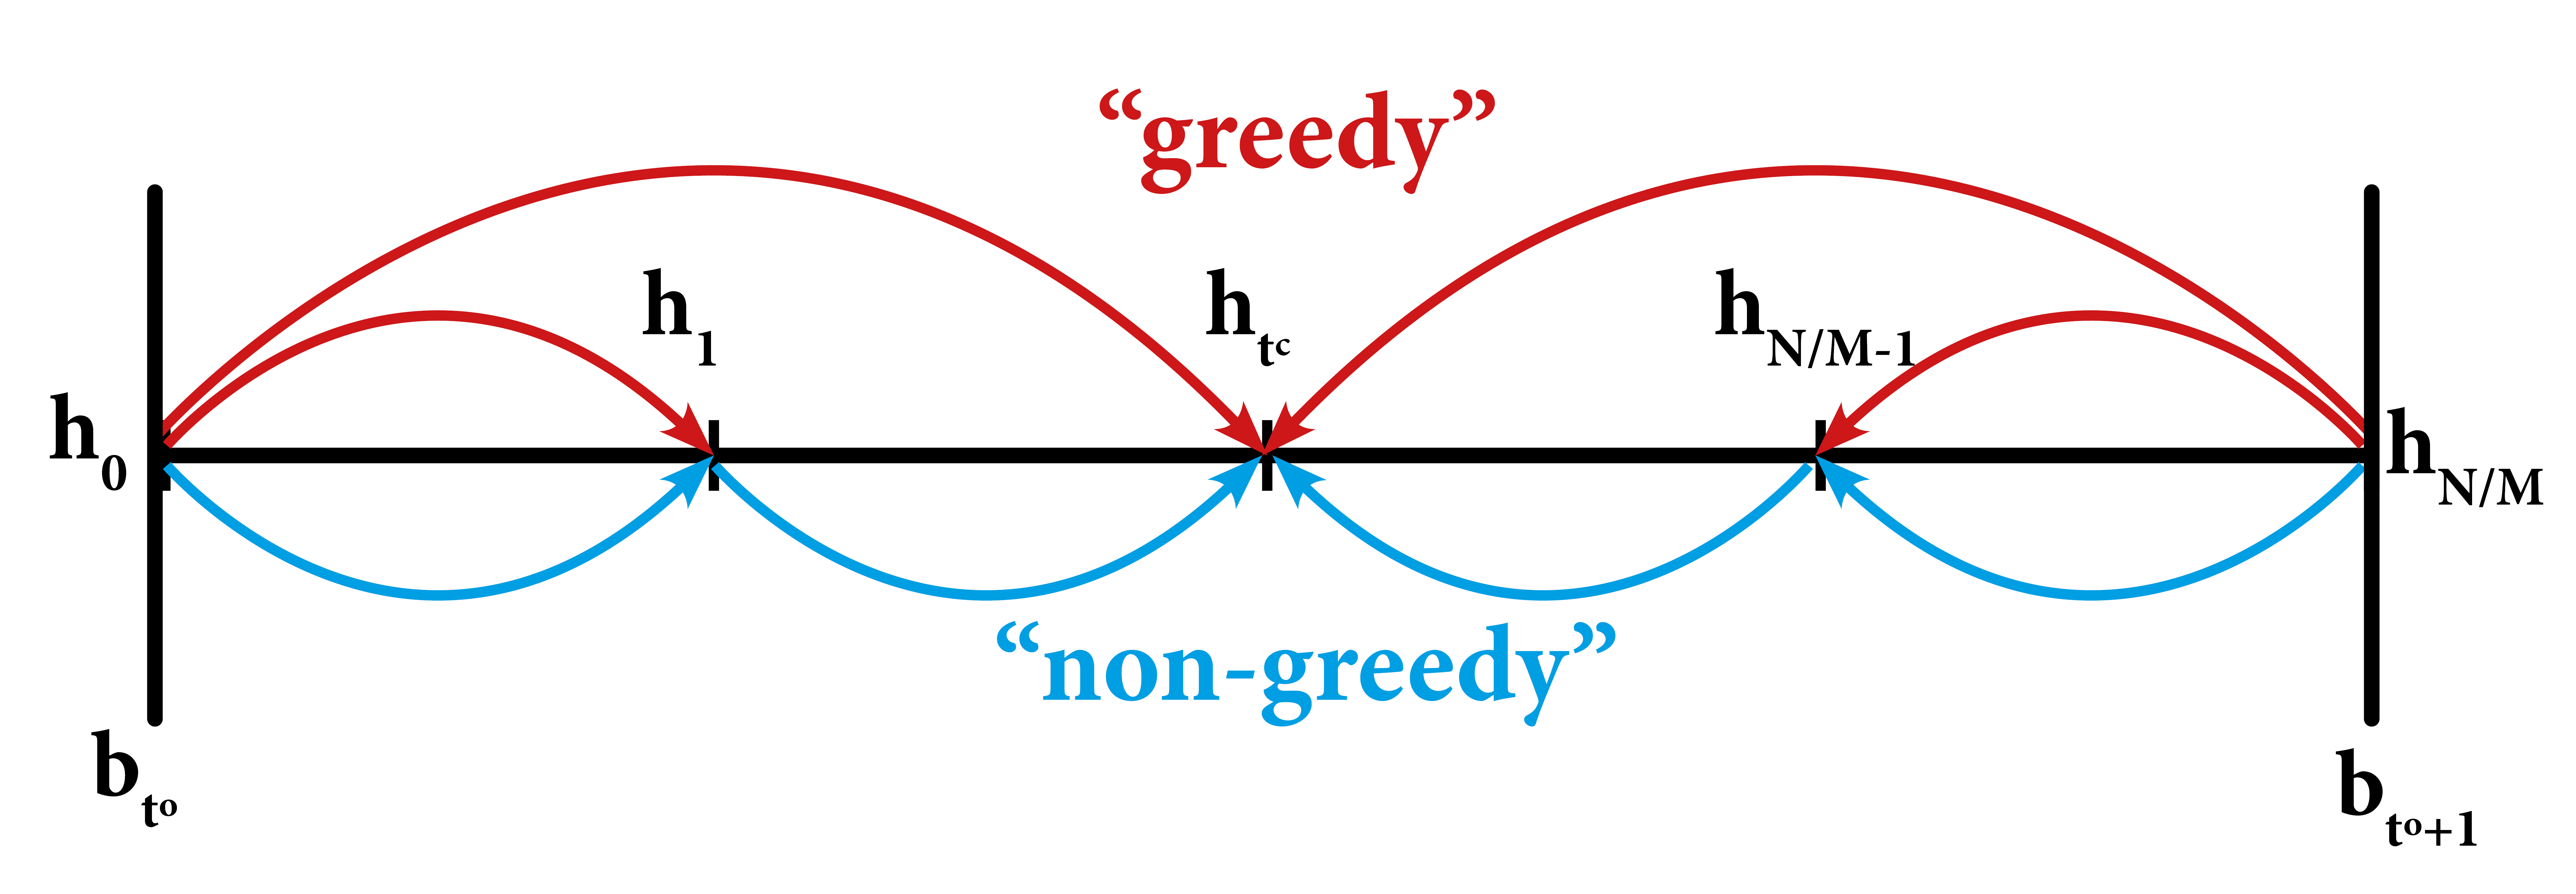
\includegraphics[width=0.8\columnwidth]{./images/NLM/propagation_scheme.png}
	\caption{\label{fig:propagation_scheme} A sketch of \textit{greedy} and \textit{non-greedy} propagation models. The two LTHS planes are at the border including small scales $ \boundHF_{t_\knot} = \h_0 $ and $ \boundHF_{t_\knot+1} = \h_{\dimth/\dimtl} $ defined in equation \ref{eq:greddy1}. All small scales to be estimated from other planes $ \h_1, \h_2,...,\h_{\dimsh/\dimsl-1} $ will be propagated either directly from LTHS planes (greedy, red arrows) or in a plane-by-plane manner (non-greedy, blue arrows). To simplify the plot, the propagation is shown from LTHS planes till the central plane only.}
\end{figure}

We propose a similarity-based model in the spirit of the NLM model for video super-resolution with important modifications. Since large scales are well reconstructed also with spline interpolation, we leave these information unchanged while propagating small scales only. Two models, the so-call ``\textit{greedy}'' and ``\textit{non-greedy}'' propagations, are proposed. Figure \ref{fig:propagation_scheme} illustrates the idea of the two propagation schemes. While the greedy model propagates small scales from LTHS planes directly toward other instant, the non-greedy one does the propagation plane-by-plane.

\subsection{Greedy propagation of small scales from key planes}
LTHS measured snapshots are crucial to recover some spatial HF contents, since these are the only place where small scales are available. In the configuration presented in figure \ref{fig:space-time_measurements}, HTLS snapshots give only information of large scales in space, while small ones are only accessible from LTHS snapshots. The idea is to bring these small-scale information and aggregate them on top of the measured large scales. The propagation model is based on the similarity of large scales at different instants, while assuming that small scales are advected by large ones.

LTHS snapshots $ \{\x_{t_\knot} \} \in \R^{\dimsh}, t_\knot = 1,2,...,\dimtl$, also called \textit{key frames}, include both large and small scales. HTLS snapshots $ \{\y_t \}  \in \R^{\dimsh}, t=1,2,...,\dimth$ contain only large scales. The propagation model aims at propagating the small-scale content from the key frames and aggregating with the interpolation $ \Interp_s\y_t $ to reconstruct $  \myhat{\z}_t $, which contains information of all scales. $ \Interp_s: \R^{\dimsl} \mymapto \R^{\dimsh} $ is the 2D cubic spline interpolator to reconstruct large scales from LR measurements. 

The propagation is based on the similarity of the large scales between the key frames and the measured planes to reconstruct. Large and small scales could be separated from the key frames using ideal Fourier filter. However, these large scales are not consistent with those from the measured planes obtained by interpolations. It is more consistent to subsample and re-interpolate LTHS fields the same way as HTLS ones. Small scales of each key frame are then defined as:
\begin{equation}
\boundHF_{t_\knot} = \mybold{x}_{t_\knot} - \Interp_s\Sub_s\mybold{x}_{t_\knot}
\label{eq:greddy1}
\end{equation}
$ \Sub_s $ is the subsampling operator in space, $ \Sub_s: \R^{\dimsh} \mymapto \R^{\dimsl} $, and $ \boundHF_{t_\knot} $ should contain some aliasing. The greedy propagation model estimates small scales $ \h_t $ at the $ t- $th time step from the given small scales  $ \boundHF_{t_\knot} $ and $ \boundHF_{t_\knot+1} $ of the two bounded LTHS planes, ones just before and after the $ t $-th HTLS plane in time:
\begin{equation}
	\hat{\h}_t[k]=\cfrac{\displaystyle \sum_{i\in\neighbor_k}w_0[k,i,t]\boundHF_{t_\knot}[i] + \sum_{i\in\neighbor_k}w_1[k,i,t]\boundHF_{t_\knot+1}[i]}{\displaystyle\sum_{i\in\neighbor_k}w_0[k,i,t] + \sum_{i\in\neighbor_k}w_1[k,i,t]}
\label{eq:greddy2}
\end{equation}
The weight $ w_0[k,i,t] $ measures the similarity of $ k-th $ pixel of $ \hat{\h}_t $ and the $ i $-th pixel of $ \boundHF_{t_\knot} $, and analogously for $ w_1[k,i,t] $. It is estimated as the similarity of large scales in the two snapshots:
\begin{equation}
w_0[k,i,t] = \myexp{ -\frac{\|\mathcal{R}_s^k\Interp_s\mybold{y}_t-\mathcal{R}_s^i\Interp_s\Sub_s\mybold{x}_{t_\knot} \|^2_2}{2\nlmfilparam^2}}
\label{eq:greddy3}
\end{equation}
The term $ \Interp_s\Sub_s\mybold{x}_{t_\knot} $ is the conjugate large scales of $ \boundHF_{t_\knot} $, i.e. $ \mybold{x}_{t_\knot} = \Interp_s\Sub_s\mybold{x}_{t_\knot} + \boundHF_{t_\knot} $. $ w_1[k,i,t] $ is estimated analogously. The final reconstruction of all scales is:
\begin{equation}
\myhat{\z}_t = \Interp_s \y_t + \myhat{\h}_t
\label{eq:greddy4}
\end{equation} 
Since $ \Interp_s \y_t $ contains some aliasing, so does $ \myhat{\h}_t $ due to the presence of aliasing in $ \boundHF_{t_\knot} $ and $ \boundHF_{t_\knot+1} $, we could hope the two aliasing terms cancel and make the estimate of $ \myhat{\z}_t $ more accurate. This can explain also the benefit when considering $ \boundHF_{t_\knot} $ as the residual of the interpolation instead of ideal small scales. 

The propagation in the formulation \ref{eq:greddy2} is point-wise, where each point is estimated as a weighted average of its neighbors. Instead, a small patch centered at $ i- $th pixel of $ \boundHF_{t_\knot} $ and $ \boundHF_{t_\knot+1} $ can be accumulated over the patch centered at the $ k- $th pixel of $ \hat{\h}_t $ using the same weights $ w_0[k,i,t] $ and $ w_1[k,i,t] $. Since the same pixel belongs to several patches, the overlapping as in the patch-based approach (section \ref{subsec:patch_based_estimation}) is used. The overlapping will ensure the continuity of neighboring points and increase the consistence of all existing structures. There will be also more degree of freedom, where the number of estimates at each location increases significantly. The accumulation of scales and weights are as:
\begin{equation}
\begin{split}
\hat{\h}_t &= \sum_{k = 1}^{\dimsh} \left( \left(\mathcal{R}_a^k\right)^{\mytrans}\left(\sum_{i\in\neighbor_k}w_0[k,i,t]\mathcal{R}_a^i\boundHF_{t_\knot}[i] + \sum_{i\in\neighbor_k}w_1[k,i,t]\mathcal{R}_a^i\boundHF_{t_\knot+1}[i]\right) \right)\\
W_t &= \sum_{k = 1}^{\dimsh} \left(\left(\mathcal{R}_a^k\right)^{\mytrans}\mathcal{R}_a^k\mybold{1} \left(\sum_{i\in\neighbor_k}w_0[k,i,t] + \sum_{i\in\neighbor_k}w_1[k,i,t]\right) \right)
\end{split}
\label{eq:greddy5}
\end{equation}
where $ \mathcal{R}_a^k $ and $ \mathcal{R}_a^i $ extract a small patch of size $ \sqrt{\dimpacc} \times \sqrt{\dimpacc} $ centered at the $ k- $th and $ i- $th pixel respectively. The transpose operator $ \left(\mathcal{R}_a^k\right)^{\mytrans} $ is to put back this small patch into the large field, centered at $ k- $th pixel. $ \mybold{1} $ is the vector of size $ \dimsh \times 1 $ of ones. The term $ \left(\mathcal{R}_a^k\right)^{\mytrans}\mathcal{R}_a^k\mybold{1} $ puts ones at the position of each patch. The whole procedure is to accumulate the sum of all small scales estimates and their corresponding weights. The final step is the normalization:
\begin{equation}
\hat{\h}_t[k] \mymapfrom \cfrac{\hat{\h}_t[k]}{W_t[k]}
\label{eq:greddy6}
\end{equation}

\subsection{Non-greedy propagation of small scales}
The greedy model aims at propagating directly small scales from the two key frames to the HTLS planes. The performance of such a model is very limited when the similarity level decays rapidly with time far from the LTHS planes. A non-greedy propagation of small-scale information plane-by-plane from the two neighboring LTHS fields toward further planes is expected to improve the reconstruction. 

\begin{algorithm}[t]
\caption{Estimating small scales of $ \dimth/\dimtl - 1 $ planes by non-greedy NLM propagation from the two key frames at $ t_\knot $ and $ t_\knot+1 $} \label{algo_NLM_timepropagation}
\begin{algorithmic}[1]
	\State Input: $ \h_0 \mydef \boundHF_{t_\knot} $, $  \h_{\dimth/\dimtl} \mydef \boundHF_{t_\knot+1} $
	\State $ t_c = round(\dimth/2\dimtl) $ \Comment{Centered snapshot}
	\For {$ i = 1, ..., t_c-1$}
		\State $ j = \dimth/\dimtl - i$
		\State $ \h_i = g(i, \h_{i - 1},\h_{j + 1})$
		\State $ \h_j = g(j, \h_{i - 1},\h_{j + 1})$
	\EndFor
	
	\If{$ rem(\dimth/\dimtl - 1) == 0 $} \Comment{Check if even, there are 2 centered snapshots}
		\State $ \h_{t_c} = g(t_c, \h_s[t_c-1],\h_s[t_c+2])$
		\State $ \h_{t_c+1} = g(t_c+1, \h_s[t_c-1],\h_s[t_c+2])$		
	\Else
		\State $ \h_{t_c} = g(t_c, \h_{t_c-1},\h_{t_c+1})$ \Comment{Estimate centered snapshot}	
	\EndIf	
\end{algorithmic}
\end{algorithm}

The main step to propagate the small scales from the two key frames at $ \boundHF_{t_\knot} $ and $ \boundHF_{t_\knot+1} $ is presented in algorithm \ref{algo_NLM_timepropagation}. $ g(t,\h_1,\h_2) $ is denoted as the similarity-based estimation of small-scale information at $ t- $th plane from the two bounded planes, with scales to propagate being $ \h_1 $ and $ \h_2 $. The procedure starts by propagating small scales from these two frames to their first two neighboring planes, $ \h_1 $ and $ \h_{\dimth/\dimtl - 1} $ in algorithm \ref{algo_NLM_timepropagation}, following the formula \ref{eq:greddy5}. The next step considers these two estimated $ \h_1 $ and $ \h_{\dimth/\dimtl - 1} $ as the new key frames and propagate them further. This procedure is repeated till the central planes that are equally far from $ \boundHF_{t_\knot} $ and $ \boundHF_{t_\knot+1} $.

\section{Applying the propagation model to isotropic turbulence}
\subsection{The choice of model parameters}
The propagation model uses several parameters (see equations \ref{eq:greddy3} and \ref{eq:greddy5}), including the filter parameter $ \sigma $, the size $ \dimpsr $,  $ \dimpsh $, and $ \dimpacc $ of the searching region $ \mathcal{N}_s $, the similarity patch extracted by $ \mathcal{R}_s $, and the accumulation patch extracted by $ \mathcal{R}_a $ respectively. Optimization of these parameters is done by varying one while fixing the remaining three. The parameter-tunning is carried out by investigating the error between the reconstructed fields and the reference ones. These tests give an idea on the optimal set of parameters, which can be used in new situations where reference fields are not available. 

\begin{table} 
	\caption{\label{tab:NLMparams}
	Set of parameters to do simple grid search (try out all possible combinations from this set): the global filter parameter $ \sigma $, size of similarity patches $ \dimpsh $, size of accumulation patches $ \dimpacc $, and size of searching region $ \dimpsr $. The search is performed on the DNS data of isotropic turbulence, with the subsampling ratios are $ \dimsh/\dimsl = 3 \times 3 $ in space and $ \dimth/\dimtl = 4 $ in time.}
	\vspace{.5cm}
	\centering
	\begin{tabular}{S[table-format=1.2]S[table-format=2.0]S[table-format=2.0]S[table-format=2.0]} 
		\toprule
		{$\sigma$} & $\sqrt{\dimpsh}$ & {$\sqrt{\dimpacc}$} & {$\sqrt{\dimpsr}$}\\ 
		\midrule 
		0.05  &  9  & 1  & 5  \\ %\addlinespace
		0.1 & 17  & 3  & 11 \\ %\addlinespace
		0.2   & 25  & 13 & 17 \\ %\addlinespace
		0.4  &    & 25 &  \\ %\addlinespace
		\bottomrule
	\end{tabular}
\end{table}

Table \ref{tab:NLMparams} gathers all parameters to test. The DNS data of isotropic turbulence are used. HTLS and LTHS measurements are virtually extracted from the fully resolved fields as discussed in section \ref{sec:probdef2}. The subsampling ratios are $ \dimsh/\dimsl = 3 \times 3 $ in space, equally distributed in spanwise and vertical direction, and $ \dimth/\dimtl = 4 $ in time (streamwise). These subsamplings correspond to energy losses of about $ 1\% $ both in space and time (see table \ref{tab:energyloss_isotropic}). The configuration is chosen to have a moderate loss of information to facilitate all numerical experiments. Other configurations with various losses are investigated later in this section.

Three measures are used to study the effects of different parameters on the reconstruction accuracy. One is the average normalized root mean square error (NRMSE) $ \bar{\epsilon} $, which represents an overall measure of the reconstruction accuracy, as in equation \ref{eq:NRMSE}. The two other quantities are the power spectra $ E(k) $ and the spectra of the error $ E^{\epsilon}(k) $. Power spectra show streamwise energy contents, while error spectra show the squared errors at each frequency. These two measures give more insights about the model performances when reconstructing turbulent fields at different scales. 

\begin{figure}[t]
	\centering
	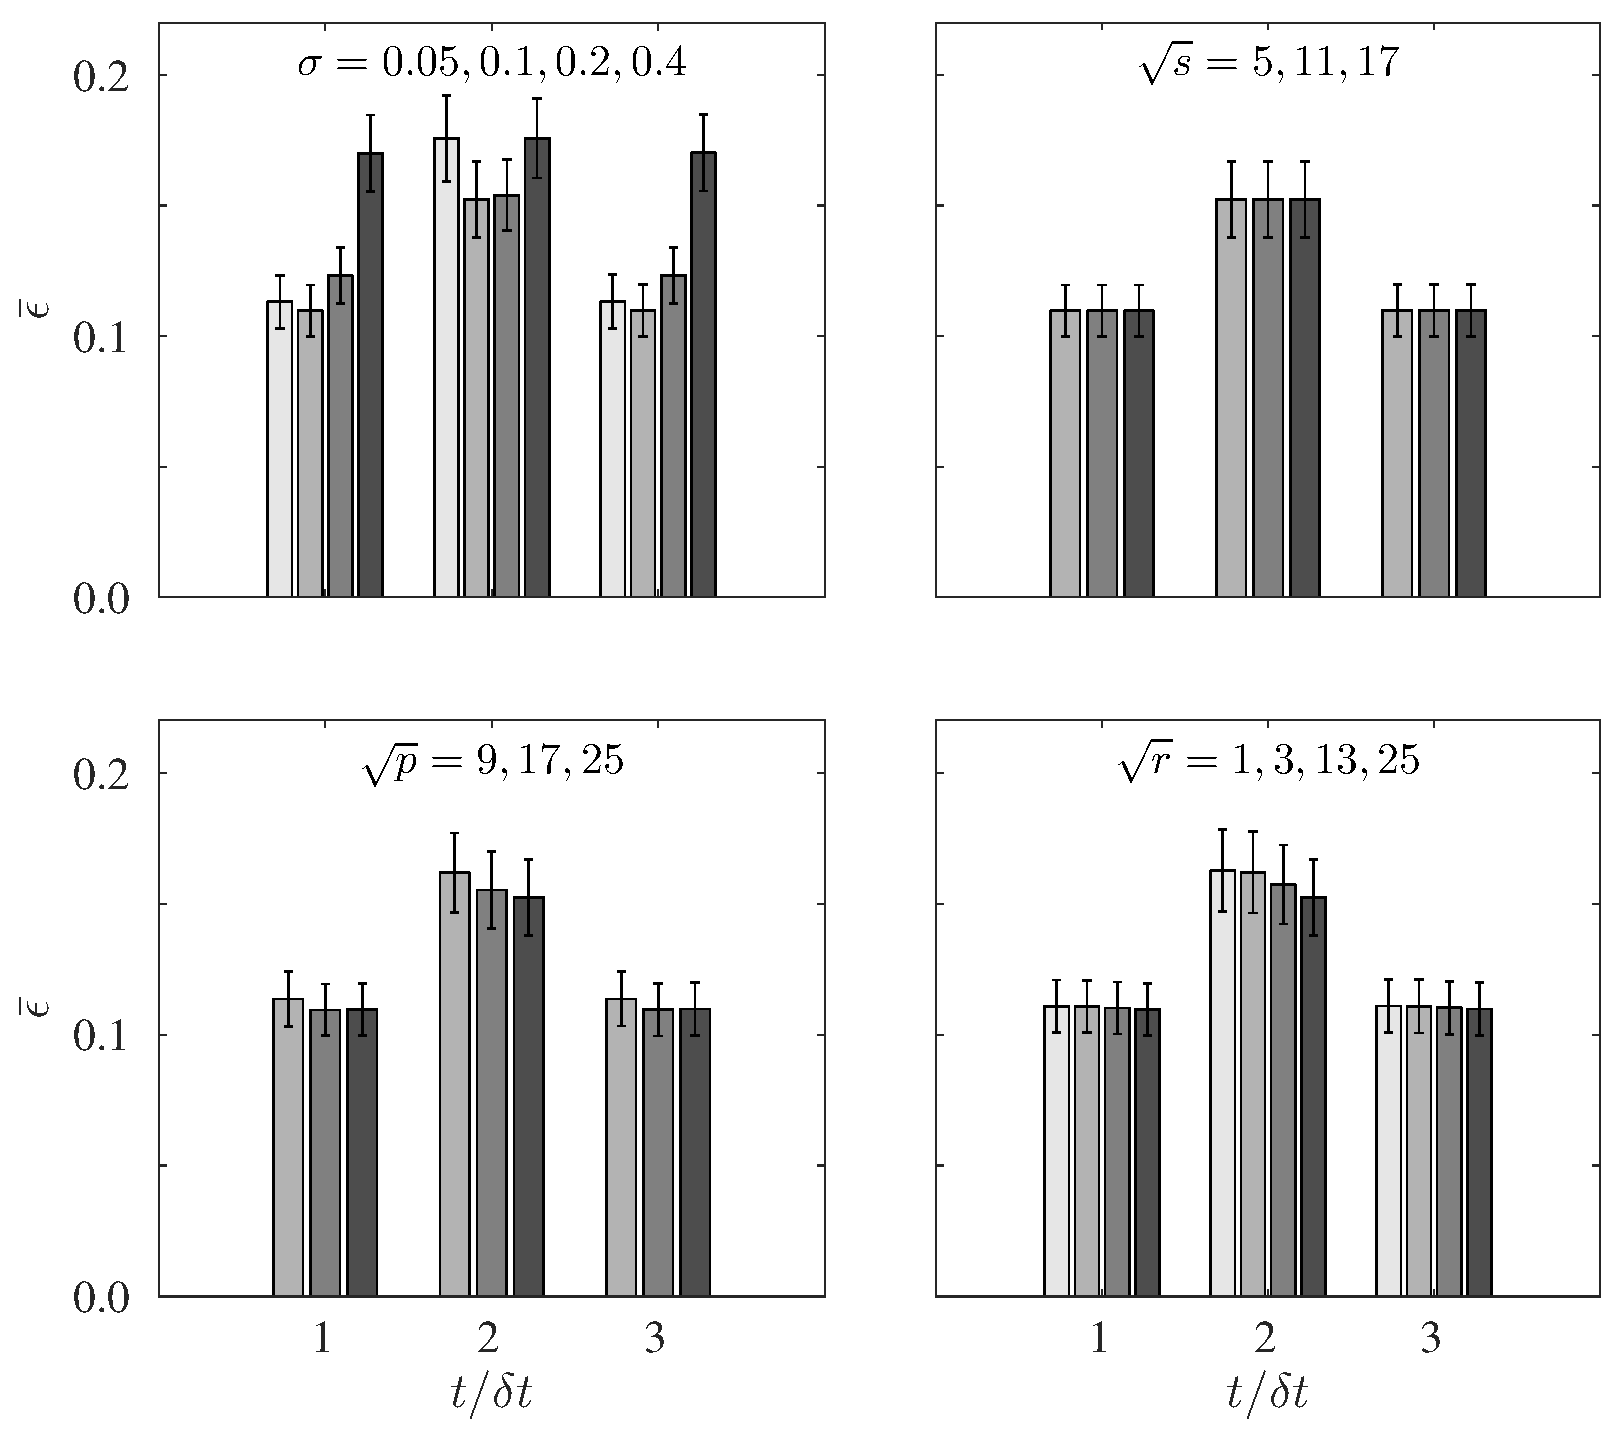
\includegraphics[width=\columnwidth]{./images/NLM/interpdiff/NLmean_propag1dir_spacing3_tspacing4_allparams_NRMSE.eps}
	\caption{\label{fig:NLM_various_params_NRMSE} Average NRMSEs over the whole dataset: each estimate of NRMSE is computed by comparing the reconstructed plane with the reference at each $ t/\delta t $. The bars show the average NRMSEs, while the error bars are standard deviations of NRMSE estimates.}
\end{figure}

Figure \ref{fig:NLM_various_params_NRMSE} shows average NRMSEs for different parameters as a function of $ t/\delta t $, the time distance from the previous LTHS plane to the estimated one. Two LTHS planes are at $ t/\delta t = 0 $ and $ t/\delta t = \dimth/\dimtl = 4 $. Average NRMSEs are shown as bars, with the standard deviation of each estimate shown by the error bars. The average and standard deviation of NRMSEs at each $ t/\delta t $ are computed using $ 37 \times 23 $ estimates from all blocks between the two successive key frames. Parameters are varied by changing one and keeping the remaining three constant around a reference parameters set ($ \sigma=0.1 $, $ \dimpsh=\dimpacc=25 \times 25 $ and $ \dimpsr = 11 \times 11$). This set is close to the optimal values used later in this section and chapter \ref{chap_comparisons} when comparing with other models.

\begin{figure}[t]
	\centering
	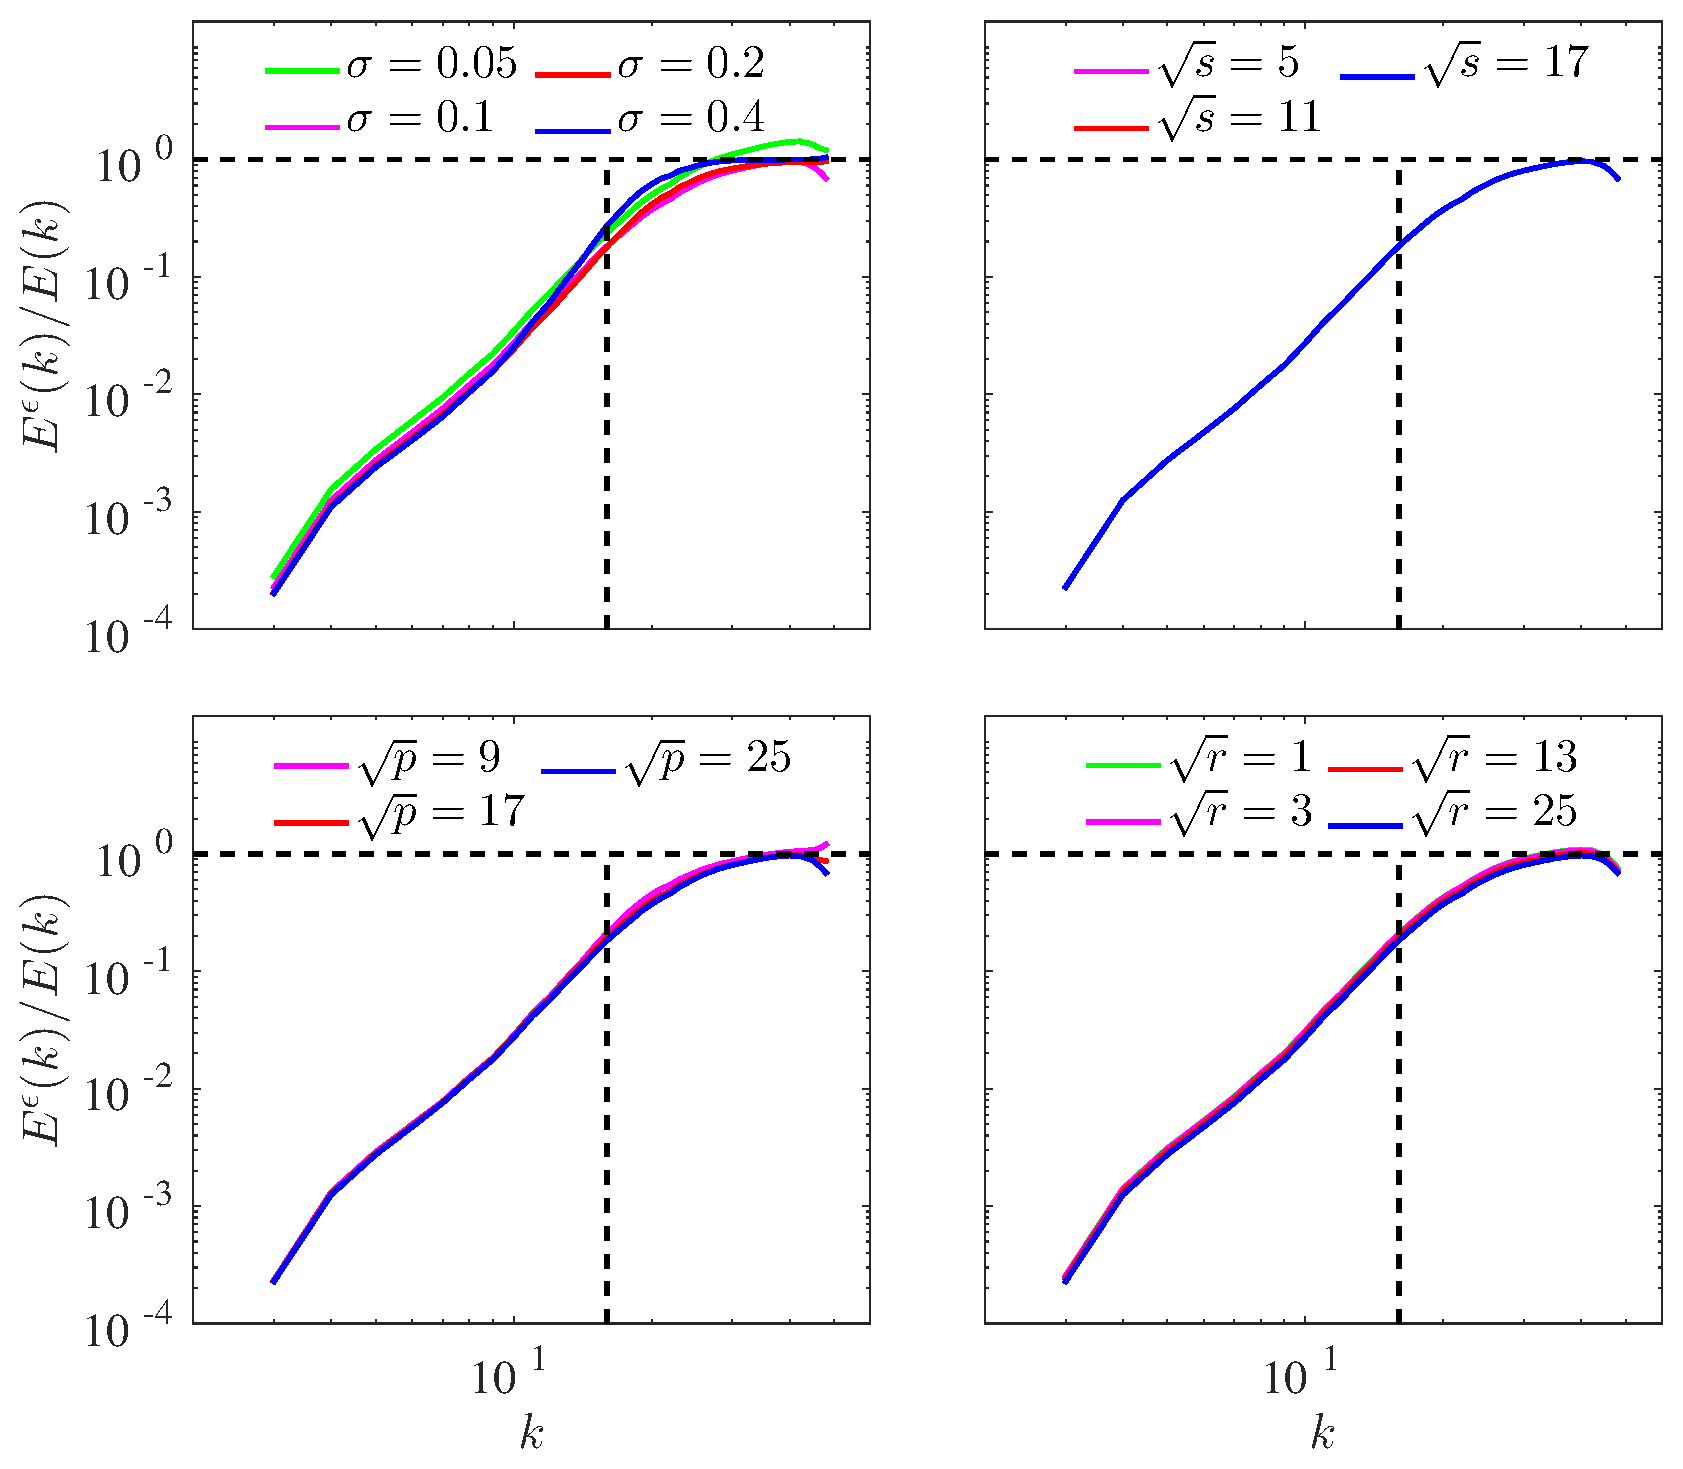
\includegraphics[width=\columnwidth]{./images/NLM/interpdiff/NLmean_propag1dir_spacing3_tspacing4_allparams_spectra.eps}
	\caption{\label{fig:NLM_various_params_spectra} Normalized error spectra of reconstructed planes at $ t/\delta t = 2 $ (the most remote from the two neighboring LTHS planes). Three cases of varying $ \dimpsh $, $\dimpacc$ and $\dimpsr$, all curves are almost collapsed.}
\end{figure}

Figure \ref{fig:NLM_various_params_spectra} shows the 2D spectra of the errors $ E^{\epsilon}(k) $ normalized by the energy spectra of the reference $ E(k) $. These spectra are estimated as an average of all planes at $ t/\delta t =2$, the most difficult planes to reconstruct. For all reconstructions, the spectra exhibit very small errors at large scales, which grow sharply when approaching the cutoff wave number defined by the spacing of the low sampling measurements. At very small scales, errors can reach $ 100 \% $. This level of error means that no information has been reconstructed. 

Among all parameters, the filter parameter $ \sigma $ is the most sensitive. The optimal value is $ \sigma \approx [ 0.1,0.2 ] $. Small values of $ \sigma $ narrow the searching region by shrinking weights of patches with low similarity levels to zero. Less estimates are taken into account when doing the weighted averaging. In the extreme situation $ \sigma = 0 $, the number of estimates is reduced to one pixel only, which is the center of the most correlated patch. The propagation model is simplified to the shifting of a single pixel. Otherwise, too large values of $ \sigma $ put weights on all the neighboring patches. Models with very large $ \sigma $ lead to a simple averaging with approximately equal weights. For these reasons, NRMSE is high for both small and large $ \sigma $, while a moderate value of $ \sigma $ is a good compromise to minimize the reconstruction error. This is shown in the error spectra (figure \ref{fig:NLM_various_params_spectra}) where the optimal $ \sigma $ gives similar large-scale reconstruction errors but lower ones at small scales.

Other model parameters are less sensitive. Searching region $ \mathcal{N}_k $ defines how large is the neighborhood to seek the small-scale information. However, the filter parameter $ \sigma $ plays a similar role by dumping the contribution of irrelevant patches to zero. Sizes of similarity and accumulation patches are more important. Similarity patches directly define the quality of weight estimates. Small patches are necessary to keep small-scale details of the flow. Larger patches improve the robustness of the models against noise and ill-posed conditions of the inverse problem. Ideally, we want the model to work well with small patches. However, experiments show slight improvements with larger patches. Similar results are observed when increasing the size of accumulation patches. Taking more pixels into the averaging helps in reducing the estimation noise, hence improving the reconstruction. 

\subsection{Comparing to spline interpolation}
The proposed propagation models, either greedy or non-greedy algorithm in time, are compared to cubic spline interpolations either in time $\Interp_t \mybold{x}_t $ or in space $\Interp_s \mybold{y}_t$. Apparently, $ \Interp_t \mybold{x}_t $ contains no temporal small-scales information, while $ \Interp_s \mybold{y}_t $ provides only large scales in space.

\begin{figure}
	\centering
	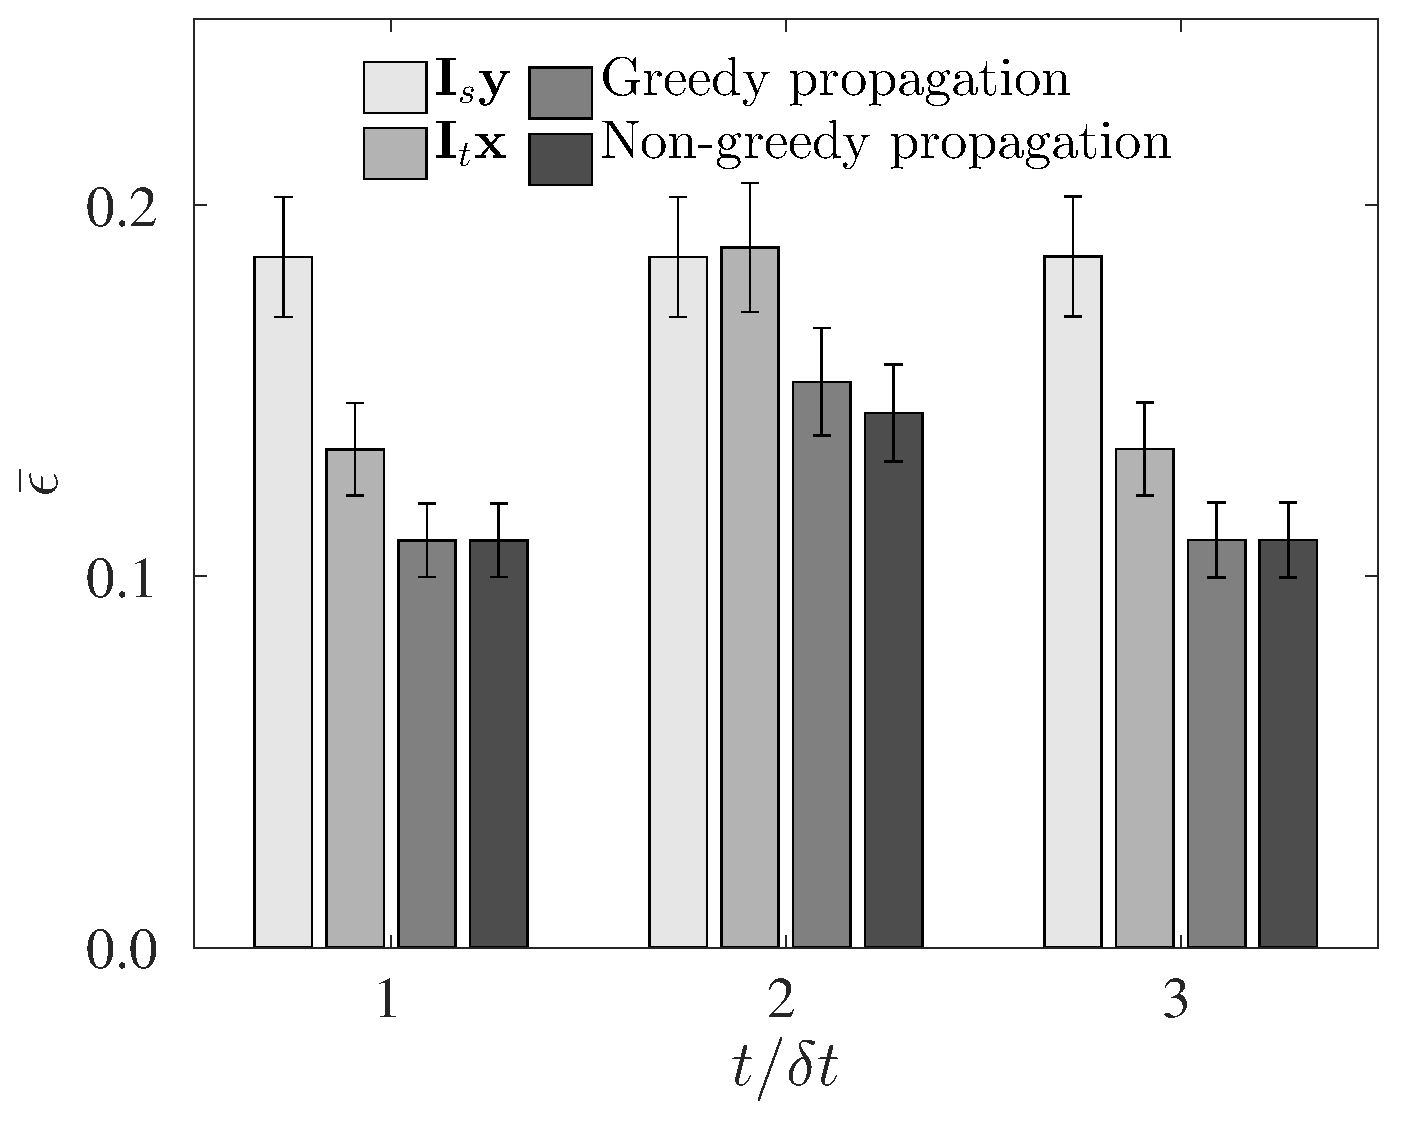
\includegraphics[width=.6\columnwidth]{./images/NLM/interpdiff/NLmean_interps_sspacing3_tspacing4_NRMSE.eps}
	\caption{\label{fig:NLmean_interps_sspacing3_tspacing4_NRMSE} Comparison of averaged NRMSEs as functions of time distances to the previous bounded LTHS plane by spatial/temporal interpolation, greedy and non-greedy propagation for the configuration where subsampling ratios are $ 3 \times 3 $ in space and $ 4 $ in time.}
\end{figure}

Figure \ref{fig:NLmean_interps_sspacing3_tspacing4_NRMSE} shows the mean NRMSEs by different methods as a function of time spacing to the previous LTHS plane $ t/\delta t $. The error bars are also shown, telling how these errors are different from one plane to another. These errors are estimated analogously as in figure \ref{fig:NLM_various_params_NRMSE}. NRMSEs of reconstructed fields obtained by propagation models or time interpolation are necessarily small close to the LTHS planes ($ t /\delta t = 1 $ and $ t /\delta t = 3 $), and increase toward the center. The error remains constant for spatial interpolation as it is only a function of the subsampling ratio in space. Greedy and non-greedy algorithms essentially give the same errors at the closest two planes from the LTHS ones. At these time steps, propagation models improve significantly (about $ 40 \% $) compared to spatial interpolation. At the middle plane, errors by propagation increase, but remain $ 20\% $ lower than both the interpolations. The non-greedy propagation model further decrease the error compared to the greedy one. 

\begin{figure}[t]
	\centering
	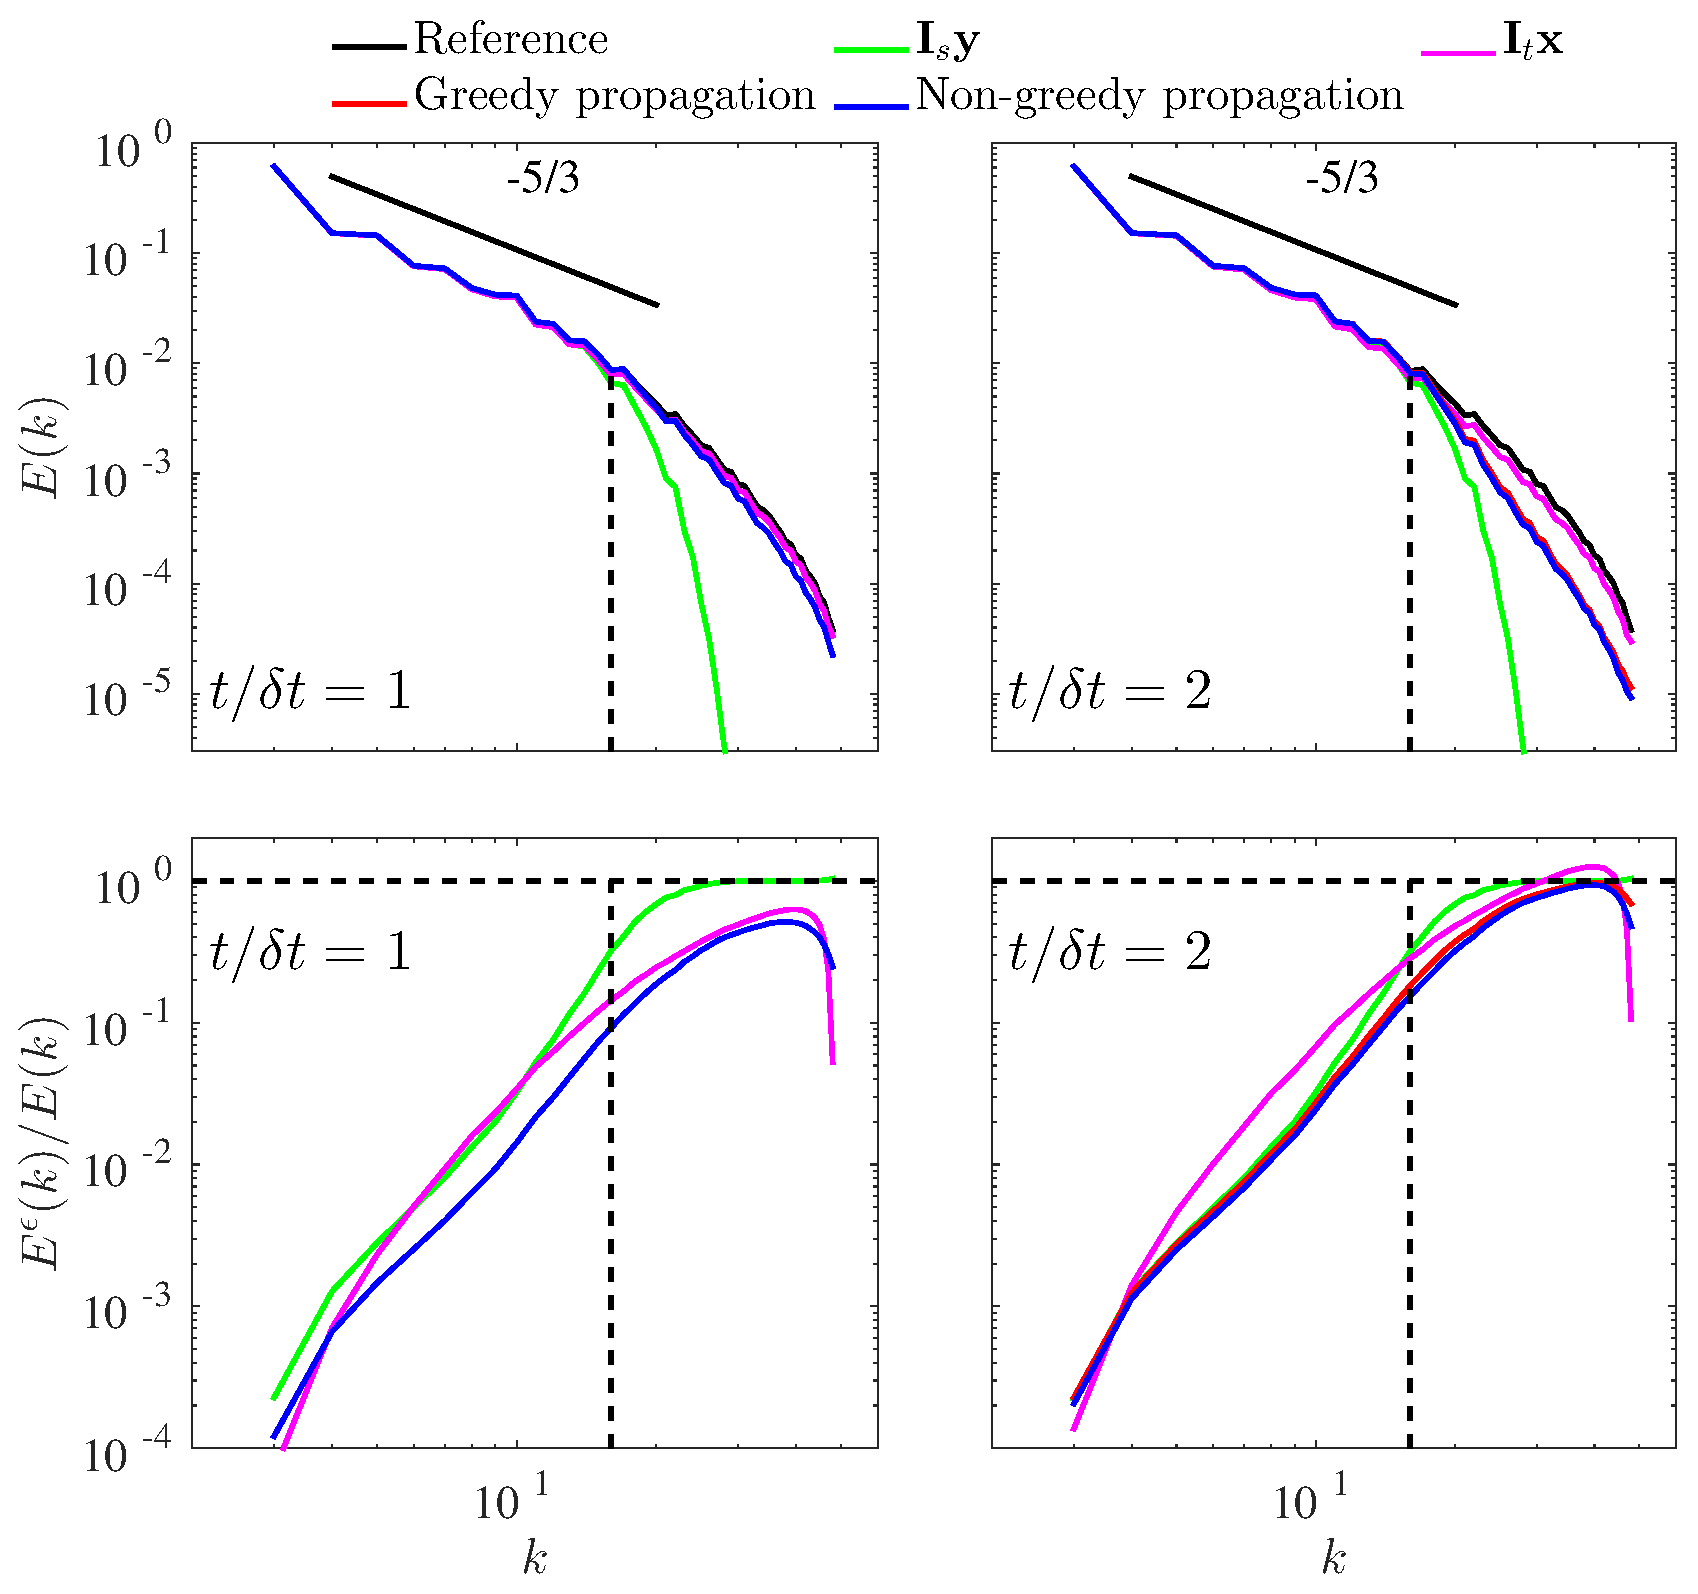
\includegraphics[width=\columnwidth]{./images/NLM/interpdiff/NLmean_interps_sspacing3_tspacing4_spectra2d.eps}		
	\caption{\label{fig:NLmean_interps_sspacing3_tspacing4_spectra2d} Comparison of energy spectra and error spectra for various reconstructions by spatial/temporal interpolation, greedy and non-greedy propagation. Subsampling ratios are $ 3 \times 3 $ in space and $ 4 $ in time. The spectra are averaged over all planes of the same distance to the closest LTHS plane, i.e. $ t/\delta t= 1 $ (left) or $t/\delta t= 2  $ (right).}
\end{figure}

Figure \ref{fig:NLmean_interps_sspacing3_tspacing4_spectra2d} shows the spectral analysis of the reconstruction by different models. Energy spectra and error spectra are shown for the two positions, either close or far from LTHS planes. From the first two spectra, it is shown that spatial interpolation captures only large-scale information. Time interpolation gives an estimate with a good energy spectrum, while propagation schemes are subject to a certain energy loss at small scales. However, the error spectra shows that time interpolation gives good energy spectra with poorly reconstructed small scales. Propagation models yield compromise estimates. Certain amount of small scales are captured, while error spectra illustrate improvements at all frequencies compared to both interpolations. 

\subsection{Model performances in various configurations}
\begin{table} 
	\caption{\label{tab:NLM_various_cases}
	Configuration parameters of six testing cases. The subsampling ratios of HTLS measurements are $ \sqrt{\dimsh/\dimsl} $ and equal in both spatial directions. The ratios of LTHS measurements in time are $ \dimth/\dimtl $. The normalized energy losses in space $\Delta\kappa_s$ and in time $\Delta\kappa_t$ are defined in Eq.~(\ref{eq:RMS_losses}).}
	\vspace{.5cm}
	\centering
	\begin{tabular}{ccS[table-format=1.0]S[table-format=1.0]cS[table-format=1.2]S[table-format=1.2]} 
		\toprule
		\multirow{2}{*}{Case}&\multicolumn{1}{c}{}&\multicolumn{2}{c}{Subsampling ratios}&\multicolumn{1}{c}{}&\multicolumn{2}{c}{Energy loss}\\ 
		\cmidrule{3-4} \cmidrule{6-7}
		 & & {$\sqrt{\dimsh/\dimsl}$} & $\dimth/\dimtl$ & & {$\Delta\kappa_s(\%)$} & {$\Delta\kappa_t (\%)$}\\ 
		\midrule 
		1 &  & 3  & 4 & & 1.03 & 1.23 \\ %\addlinespace
		2 &  & 3  & 6 & & 1.03 & 3.56 \\ %\addlinespace
		3 &  & 3  & 8 & & 1.03 & 6.53 \\ %\addlinespace
		4 &  & 3  & 4 & & 1.03 & 1.23 \\ %\addlinespace
		5 &  & 4  & 4 & & 2.63 & 1.23 \\ %\addlinespace	 
		6 &  & 6  & 4 & & 7.29 & 1.23 \\ %\addlinespace
		\bottomrule
	\end{tabular}
\end{table}

To characterize the proposed propagation models, various configurations at different subsampling ratios in either space or time are investigated. Model performances depend on the ratio in space, since it defines how much information is missing. The performances also depend on the ratio in time, since small-scale information will necessarily be lost when similarity between large scales die off with increasing time spacings. 

\begin{figure}[t]
	\centering
	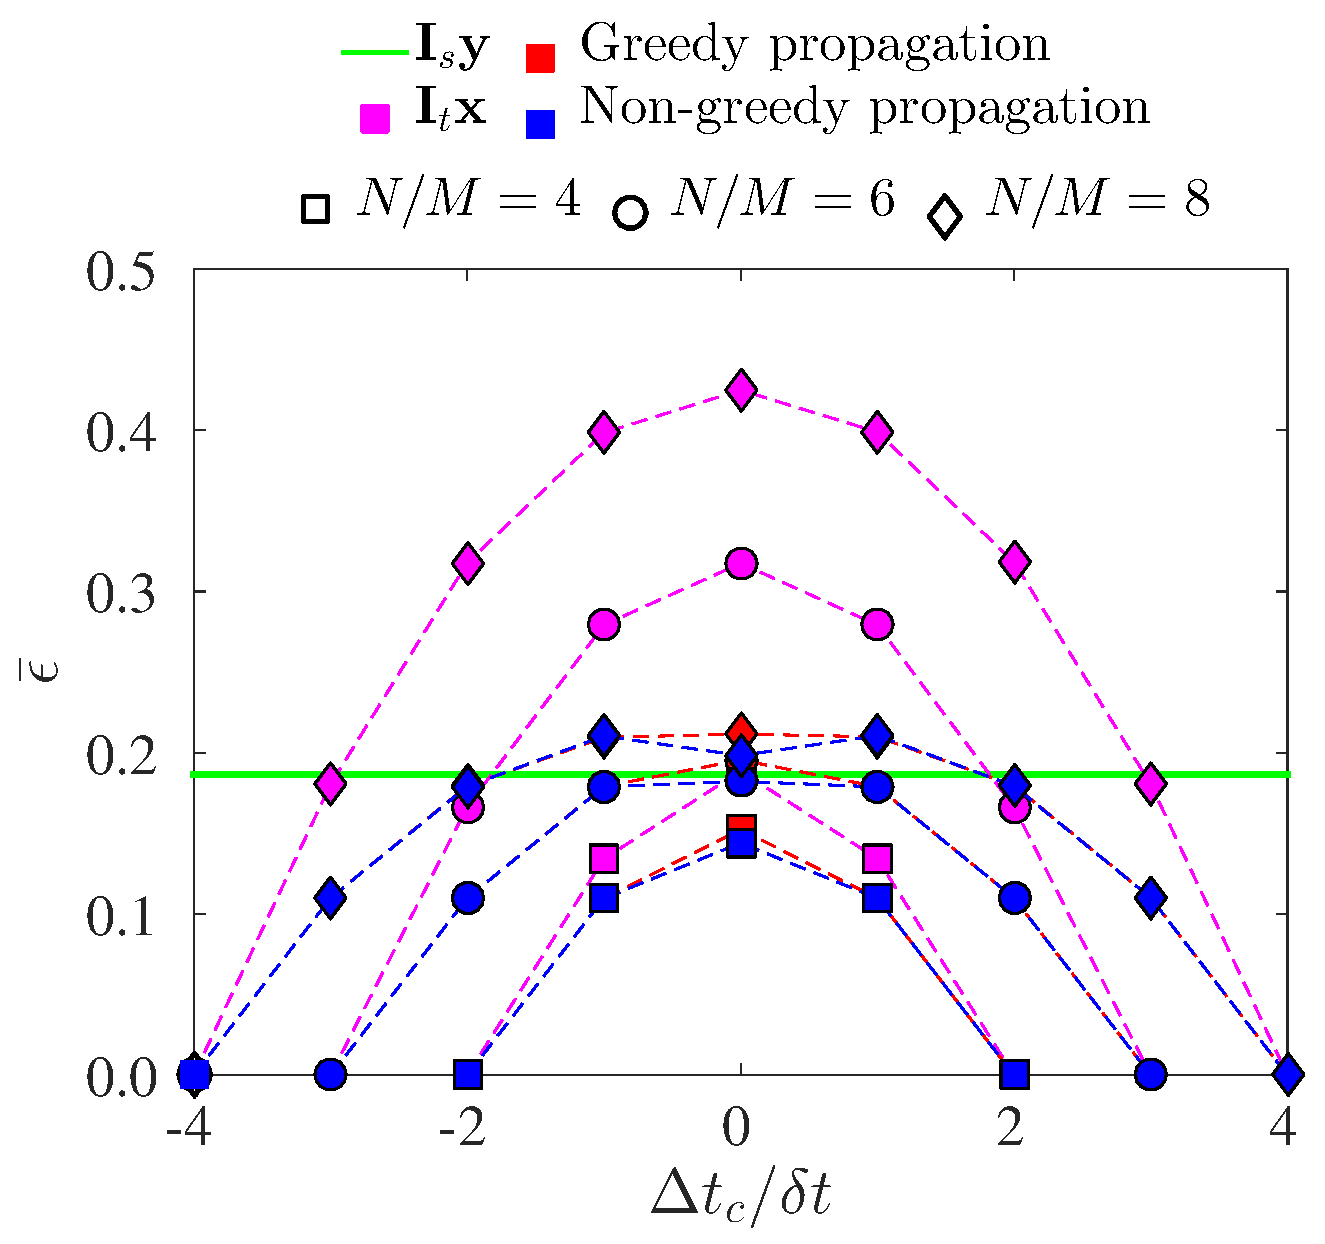
\includegraphics[width=0.65\columnwidth]{./images/NLM/interpdiff/NLmean_interps_NRMSE_vary_timespacing.eps}		
	\caption{\label{fig:NLmean_interps_NRMSE_vary_timespacing} Averaged NRMSEs of reconstruction by spatial/temporal interpolation, greedy and non-greedy propagation models. The errors are shown for three cases, with a fixed ratio in space $ (\dimsh/\dimsl = 3 \times 3) $ and varied ratios in time $(\dimth/\dimtl=4,6,8) $. The reference plane is chosen to be the mid-plane, and $ \Delta t_c/\delta t $ is the distance of each other plane from the reference one. Different colors refer to different methods, while the marker shapes vary for different $ \dimth/\dimtl $.}
\end{figure}

To test the model performances when increasing time distances between LTHS snapshots, the subsampling ratio $ \dimsh/\dimsl=3 \times 3 $ in space, while varying those in time as $ \dimth/\dimtl=4,6 $ and $ 8 $. The amount of missing information to recover due to the subsampling in space is about $ 1 \% $ of the total energy of the flow. Average NRMSEs as a function of the position in time are shown in figure \ref{fig:NLmean_interps_NRMSE_vary_timespacing}. In all three cases, the central plane is at $ \Delta t_c/\delta t = 0 $, while other planes are at different distances $ \Delta t_c/\delta t$ to this plane, both negative (planes before) or positive (plane after). 

In the figure \ref{fig:NLmean_interps_NRMSE_vary_timespacing}, NRMSE for spatial interpolation remains constant, since it is independent of time. Errors by time interpolations or propagation models increase when moving toward the center. For time interpolations, these errors increase dramatically when the time subsampling ratio is high. The proposed propagation models are able to bring down the errors compared to interpolation for small to moderate distances between LTHS planes. For very large ones ($ \dimth/\dimtl=8 $, diamond shape), the propagated small scales even slightly downgrade the given large-scale information from the spatial interpolation.

\begin{figure}[t]
	\centering
	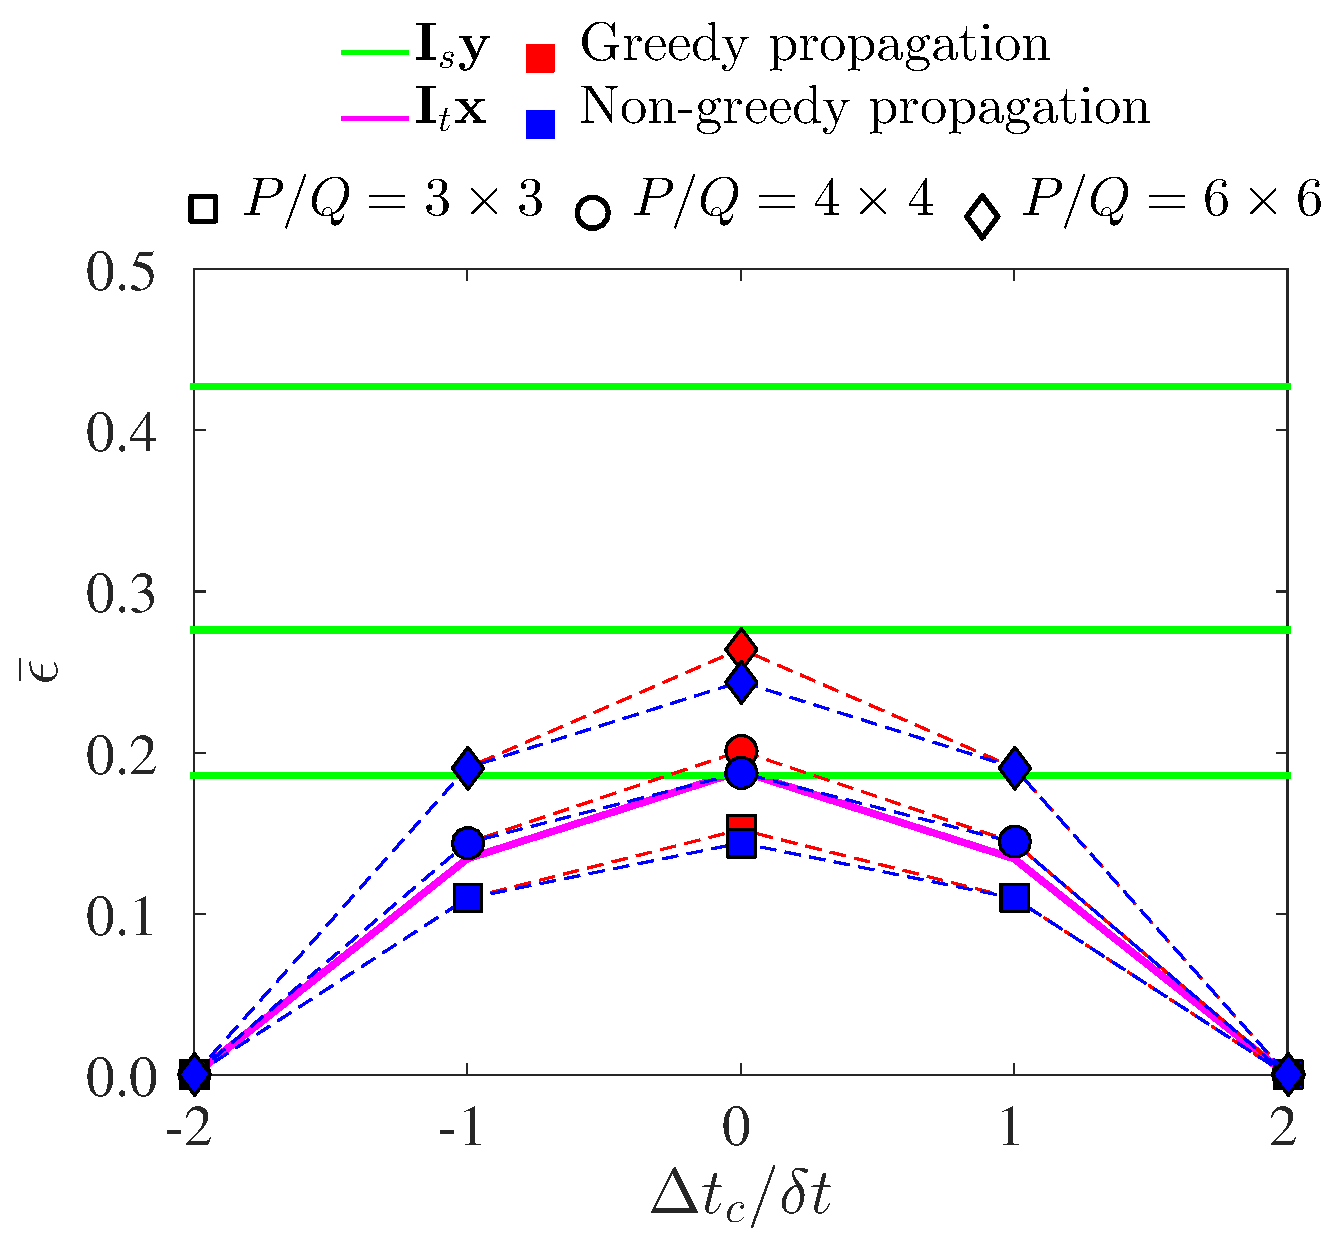
\includegraphics[width=0.65\columnwidth]{./images/NLM/interpdiff/NLmean_interps_NRMSE_vary_spacespacing.eps}		
	\caption{\label{fig:NLmean_interps_NRMSE_vary_spacespacing} Averaged NRMSEs of reconstruction by spatial/temporal interpolation, greedy and non-greedy propagation models. The errors are shown for different space spacing $ (\dimsh/\dimsl=3 \times , 4 \times 4, 6 \times 6) $, while in time the ratio is fixed $ (\dimth/\dimtl =4) $. The reference plane is chosen to be the mid-plane, and $ \Delta t_c/\delta t $ is the distance of each other plane from the reference one. Different colors refer to different methods, while the marker shapes vary for different $ \dimsh/\dimsl $.}
\end{figure}

Figure \ref{fig:NLmean_interps_NRMSE_vary_spacespacing} shows NRMSEs of the proposed propagation models (both greedy and non-greedy), spatial and temporal interpolations when varying the subsampling ratio in space as $ \dimsh/\dimsl = 3 \times 3, 4 \times 4 $ and $ 6 \times 6 $ while keeping a fixed distance between LTHS planes of $ \dimth/\dimtl=4 $. Time interpolation gives the same error for all three cases, while errors of spatial interpolations are independent of the position in time. For a small subsampling ratio in time, temporal interpolation and propagation models are always better than spatial interpolation. For a small ratio of $ \dimsh/\dimsl = 3 \times 3 $, the non-greedy propagation scheme give the most accurate reconstruction. In the case of moderate ratio ($ \dimsh/\dimsl=4 \times 4 $), the energy loss in space is already three times larger than that in time (see table \ref{tab:NLM_various_cases}). Propagation models start with large scales from spatial interpolation and reconstruct small-scale information to give the same accuracy as time interpolation. For a large subsampling ratio of $ \dimsh/\dimsl = 6 \times 6 $, propagation models improves significantly compared to spatial interpolation but remains worse than temporal interpolation. This is due to severe information losses after the subsampling in space, which cannot be  completely recovered.

\section{Concluding remarks}
The similarity-based propagation model, also called NLM-based propagation model, is proposed to reconstruct small scales in a configuration where measurements of all scales are given at key frames (LTHS planes). Small scales from these planes are propagated toward other instants in time. The proposed model takes benefits from the local/nonlocal similarity among scales and  among neighboring fields. Large-scale information is used as initial estimates and kept unchanged, while small scales are propagated as a weighted sum within a small neighborhood from one plane to another. The weights are estimated as the similarity of large scales in small patches. They are interpreted as the probabilities of an estimate to be its neighbors from nearby planes or key frames. 

The model works very well in the situation where the subsampling ratios are not severe. In such case, it is able to bring small scales of the flow and add to initial large scales given by the coarse measurements. It also performs better than temporal interpolation from key frames, which is point-wise and disregards the spatial structures of the flow. Among the models, the non-greedy propagation works the most accurately by gradually bringing small-scale information from the bounded planes toward the center. 

This model is not robust when the subsampling ratios remain moderate. When the time distance between LTHS planes increases, model performances are getting worse than spatial interpolation. This is because when the key frames are far from each other, similarities of large scales decay, making propagation models becomes inefficient. Reconstructed small-scale information even downgrades the initial large scales from spatial interpolation. The discrepancies are also found with large subsampling ratios in space. In such cases, the model suffers from severe information loss that can not be recovered completely. 

More sophisticated models can be further investigated to improve the reconstruction. First, it's worth mentioning the idea of multi-scale propagation, which has been investigated during this work but gives no improvement. However, in the case where the range of scales is extremely wide, there might be potential gain from a non-greedy propagation in space as the one in time presented in this chapter. Second, since structures in turbulence distort and rotate in a disorder manner, it maybe better to propose adapted methods that compute similarity of rotating patches. This idea has been started by \citet{zimmer2008rotationally}, but further investigation is required to adapt to our problem.



\chapter{Bayesian framework}
\label{apx_BayesGausvars}

\section{Derivation of Linear Gaussian models}
\label{apx_BayesGausvars_1}
\subsection{Bayes' theorem for Gaussian variables}
Let $ \mybold{v} $ is the measurement, then the probability $ p(\mybold{v}) $ is known. Let $ \mybold{u} $ is the desired variable, with the prior distribution $ p(\mybold{u}) $. Suppose also there exists a linear observation model:
\begin{equation}
	\mybold{v}=A\mybold{u}+\mybold{n}
\label{eq:LG5}
\end{equation}
where $ \mybold{n} $ is a zero-mean random vectors and independent on $ \mybold{u} $ and $ \mybold{v} $ and has a precision matrix denoted as $ \Lambda_{\mybold{v}|\mybold{u}}= \Sigma_{\mybold{v}|\mybold{u}}^{-1}$. One can express the joint probability $ p(\mybold{w})$ as the product of the prior probability $ p(\mybold{u}) $ and the likelihood function of the measurement given the variable $ p(\mybold{v}|\mybold{u})$ as:
\begin{eqnarray}
	p(\mybold{u})=&&\distr(\mybold{u}|\mybold{\mu}_{\mybold{u}},\Lambda^{-1}_{\mybold{u}}) \\
	p(\mybold{v}|\mybold{u})=&&\distr(\mybold{v}|A\mybold{\mu}_{\mybold{u}},\Lambda_{\mybold{v}|\mybold{u}}^{-1})
\label{eq:LG6}
\end{eqnarray}
To derive, let take the natural logarithm of both sides, using also the symmetrical shape of precision matrices,  the left hand side gives:
\begin{eqnarray}
	ln \: p(\mybold{w}) =&& -\frac{1}{2} \left(\mybold{w}-\mybold{\mu}_{\mybold{w}} \right)^T \Lambda_{\mybold{w}} \left(\mybold{w}-\mybold{\mu}_{\mybold{w}} \right) + const \nonumber\\
	=&& -\frac{1}{2} \mybold{w}^T \Lambda_{\mybold{w}} \mybold{w} +\mybold{w}^T \Lambda_{\mybold{w}} \mybold{\mu}_{\mybold{w}} \nonumber\\
	&& - \frac{1}{2} \mybold{\mu}_{\mybold{w}} \Lambda_{\mybold{w}} \mybold{\mu}_{\mybold{w}} + const
	\label{eq:LG7}
\end{eqnarray}
and the right hand side gives:
\begin{eqnarray}
	ln \left(p(\mybold{u}) p(\mybold{v}|\mybold{u}) \right) =&& \left(\mybold{u}-\mybold{\mu}_{\mybold{u}} \right)^T \Lambda_{\mybold{u}} \left(\mybold{u}-\mybold{\mu}_{\mybold{u}} \right) \nonumber\\
	&&- \frac{1}{2} \left( \mybold{v}-A\mybold{u} \right)^T \Lambda_{\mybold{v}|\mybold{u}} \left( \mybold{v}-A\mybold{u} \right) \nonumber\\
	&&+ const
\label{eq:LG8}
\end{eqnarray}
In above equations, $ const $ represents all the terms that are independent on $ \mybold{u} $ and $\mybold{v}$. The first order terms in the above equation include:
\begin{eqnarray}
	1^{st} \: order \: terms =&& \mybold{u}^T  \Lambda_{\mybold{u}} \mybold{\mu}_{\mybold{u}} - \mybold{u}^T A^T\Lambda_{\mybold{v}|\mybold{u}} \nonumber\\
	=&&  \left(\begin{matrix}\mybold{u}\\\mybold{v} \end{matrix}\right)^T  \left(\begin{matrix}\Lambda_{\mybold{u}}{\mu}_{\mybold{u}} \\ 0 \end{matrix}\right)
\label{eq:LG9}
\end{eqnarray}
and the second order terms are:
\begin{eqnarray}
	2^{nd} \: order \: terms = && -\frac{1}{2} \mybold{u}^T \left( \Lambda_{\mybold{u}}+A^T \Lambda_{\mybold{v}|\mybold{u}} A \right)\mybold{u}  - \frac{1}{2} \mybold{v}^T \Lambda_{\mybold{v}|\mybold{u}} \mybold{v} \nonumber\\
	&& + \frac{1}{2} \mybold{v}^T \Lambda_{\mybold{v}|\mybold{u}} A \mybold{u} + \mybold{u}^T A^T \Lambda_{\mybold{v}|\mybold{u}} \mybold{v} \nonumber\\
	=&& -\frac{1}{2} \left(\begin{matrix}\mybold{u}\\\mybold{v} \end{matrix}\right)^T  \left(\begin{matrix}A^T\Lambda_{\mybold{v}|\mybold{u}}A+\Lambda_{\mybold{u}} & A^T\Lambda_{\mybold{v}|\mybold{u}} \nonumber\\ -\Lambda_{\mybold{v}|\mybold{u}} A & \Lambda_{\mybold{v}|\mybold{u}}\end{matrix}\right) \left(\begin{matrix}\mybold{u}\\\mybold{v} \end{matrix}\right) \\
	=&& -\frac{1}{2} \mybold{w}^T \Lambda_{\mybold{w}} \mybold{w}
\label{eq:LG10}
\end{eqnarray}
Comparing above equations \ref{eq:LG10}, \ref{eq:LG9} and \ref{eq:LG7}, Gaussian distribution of $ \mybold{w} $ takes the precision matrix $ \Lambda_{\mybold{w}} $ of the form:
\begin{equation}
	\Lambda_{\mybold{w}}= \left(\begin{matrix}\Lambda_{\mybold{u}\mybold{u}} & \Lambda_{\mybold{u}\mybold{v}} \\ \Lambda_{\mybold{v}\mybold{u}} & \Lambda_{\mybold{v}\mybold{v}}\end{matrix}\right) = \left(\begin{matrix}A^T\Lambda_{\mybold{v}|\mybold{u}}A+\Lambda_{\mybold{u}} & A^T\Lambda_{\mybold{v}|\mybold{u}} \\ -\Lambda_{\mybold{v}|\mybold{u}} A & \Lambda_{\mybold{v}|\mybold{u}}\end{matrix}\right)
\label{eq:LG11}
\end{equation}
and the mean $ \mybold{\mu}_{\mybold{w}} $ is:
\begin{equation}
	\mybold{\mu}_{\mybold{w}} = \left(\begin{matrix}\mybold{\mu}_{\mybold{u}} \\ \mybold{\mu}_{\mybold{v}} \end{matrix}\right) = \Lambda_{\mybold{w}}^{-1}\left(\begin{matrix}\Lambda_{\mybold{u}}\mybold{\mu}_{\mybold{u}} \\ 0 \end{matrix}\right) =\Sigma_{\mybold{w}} \left(\begin{matrix}\Lambda_{\mybold{u}}\mybold{\mu}_{\mybold{u}} \\ 0 \end{matrix}\right)
\label{eq:LG12}
\end{equation}
The covariance matrix is obtained by taking the inverse of above:
\begin{equation}
	\Sigma_{\mybold{w}}=\left(\begin{matrix}\Sigma_{\mybold{u}\mybold{u}} & \Sigma_{\mybold{u}\mybold{v}} \\ \Sigma_{\mybold{v}\mybold{u}} & \Sigma_{\mybold{v}\mybold{v}}\end{matrix}\right) = \left(\begin{matrix}A^T\Lambda_{\mybold{v}|\mybold{u}}A+\Lambda_{\mybold{u}} & A^T\Lambda_{\mybold{v}|\mybold{u}} \\ -\Lambda_{\mybold{v}|\mybold{u}} A & \Lambda_{\mybold{v}|\mybold{u}}\end{matrix}\right)^{-1} 
\label{eq:LG13}
\end{equation}
Using the inversion lemma:
\begin{equation}
	\left(\begin{matrix} A & B \\ C & D \end{matrix}\right)^{-1}= \left(\begin{matrix}M & -MBD^{-1} \\ D^{-1}+D^{-1}CM & D^{-1}CMBD^{-1}\end{matrix}\right)
\label{eq:LG14}
\end{equation}
where $ M=(A-BD^{-1}C)^{-1} $ is the \textit{Schur complement} of the matrix inversion with respect to $ D $. The covariance matrix is finally given as:
\begin{equation}
	\Sigma_{\mybold{w}}= \left(\begin{matrix}\Sigma_{\mybold{u}\mybold{u}} & \Sigma_{\mybold{u}\mybold{v}} \\ \Sigma_{\mybold{v}\mybold{u}} & \Sigma_{\mybold{v}\mybold{v}}\end{matrix}\right) =\left(\begin{matrix}\Lambda^{-1}_{\mybold{u}} & \Lambda^{-1}_{\mybold{u}}A^T \\ A \Lambda^{-1}_{\mybold{u}} &\Lambda^{-1}_{\mybold{v}|\mybold{u}} + A\Lambda^{-1}_{\mybold{u}}A^T\end{matrix}\right)
\label{eq:LG15}
\end{equation}
Replacing this covariance matrix to equation (\ref{eq:LG13}), the expectation of $ \mybold{w} $ is given as:
\begin{equation}
	\mybold{\mu}_{\mybold{w}} = \left(\begin{matrix}\mybold{\mu}_{\mybold{u}} \\ \mybold{\mu}_{\mybold{v}} \end{matrix}\right) =\left(\begin{matrix}\Lambda^{-1}_{\mybold{u}} & \Lambda^{-1}_{\mybold{u}}A^T \\ A \Lambda^{-1}_{\mybold{u}} & \Lambda^{-1}_{\mybold{v}|\mybold{u}} + A\Lambda^{-1}_{\mybold{u}}A^T\end{matrix}\right) \left(\begin{matrix}\Lambda_{\mybold{u}}\mybold{\mu}_{\mybold{u}} \\ 0 \end{matrix}\right) = \left(\begin{matrix}\mybold{\mu}_{\mybold{u}} \\ A\mybold{\mu}_{\mybold{u}} \end{matrix}\right)
\label{eq:LG16} 
\end{equation}
From equation \ref{eq:LG15} and \ref{eq:LG16}, the Gaussian distribution of $ \mybold{v} = \distr(\mybold{v}| \mybold{\mu}_{\mybold{v}},\Sigma_{\mybold{v}}) $ is:
\begin{eqnarray}
	\mybold{\mu}_{\mybold{v}} =&& A\mybold{\mu}_{\mybold{u}} \nonumber\\
	\Sigma_{\mybold{v}} =&& \Lambda^{-1}_{\mybold{v}|\mybold{u}} + A\Lambda^{-1}_{\mybold{u}}A^T
\label{eq:LG17}
\end{eqnarray}
Using results of conditional Gaussian distribution as in equation \ref{eq:LG4}, the posterior ditribution $ \mybold{u}|\mybold{v} $ is $ \distr \left(\mybold{u}|\mybold{\mu}_{\mybold{u}|\mybold{v}}, \Sigma_{\mybold{u}|\mybold{v}} \right) $ where:
\begin{eqnarray}
	\mybold{\mu}_{\mybold{u}|\mybold{v}} =&& \mybold{\mu}_{\mybold{u}}-\Lambda^{-1}_{\mybold{u}\mybold{u}} \Lambda_{\mybold{u}\mybold{v}} (\mybold{u}-\mybold{\mu}_{\mybold{u}}) \nonumber\\
	\Sigma_{\mybold{u}|\mybold{v}} =&& \Lambda^{-1}_{\mybold{u}\mybold{u}}
\label{eq:LG18}
\end{eqnarray}
Taking the partial precision matrices from equation \ref{eq:LG11}, covariance matrix $ \Sigma_{\mybold{u}|\mybold{v}} $ is given as:
\begin{equation}
	\Sigma_{\mybold{u}|\mybold{v}}= \left(A^T\Lambda_{\mybold{v}|\mybold{u}}A+\Lambda_{\mybold{u}}\right)^{-1} 
\label{eq:LG19}	
\end{equation}
and conditional mean $ \mybold{\mu}_{\mybold{u}|\mybold{v}} $ is as:
\begin{eqnarray}
	\mybold{\mu}_{\mybold{u}|\mybold{v}} =&& \mybold{\mu}_{\mybold{u}}- \left(	A^T\Lambda_{\mybold{v}|\mybold{u}}A+\Lambda_{\mybold{u}} \right) ^{-1} \left( -A^T\Lambda_{\mybold{v}|\mybold{u}} \right) \left( \mybold{v}- A\mybold{\mu}_{\mybold{u}} \right) \nonumber\\
	=&& \left(	A^T\Lambda_{\mybold{v}|\mybold{u}}A+\Lambda_{\mybold{u}} \right)^{-1} \left(	A^T\Lambda_{\mybold{v}|\mybold{u}} \mybold{v} +\Lambda_{\mybold{u}}\mybold{\mu}_{\mybold{u}} \right)
\label{eq:LG20}
\end{eqnarray}
Final results written in covariance matrices notation, given:
\begin{eqnarray}
	\mybold{v} =&& A\mybold{u} \nonumber\\
	p(\mybold{u}) =&& \distr \left( \mybold{u}| \mybold{\mu}_{\mybold{u}},\Sigma_{\mybold{u}} \right) \nonumber\\
	p(\mybold{v}|\mybold{u}) =&& \distr \left( \mybold{v}| A\mybold{u},\Sigma_{\mybold{v}|\mybold{u}} \right)
\label{eq:LG21}	
\end{eqnarray}
one gets:
\begin{eqnarray}
	p(\mybold{v}) =&& \distr \left( \mybold{v}| A\mybold{\mu}_{\mybold{u}},\Sigma_{\mybold{v}|\mybold{u}} +A\Sigma_{\mybold{u}}  A^T \right) \nonumber\\
	p(\mybold{u}|\mybold{v}) =&& \distr \left( \mybold{u}| \Sigma_{\mybold{u}|\mybold{v}} \left(	A^T\Lambda_{\mybold{v}|\mybold{u}} \mybold{v} +\Lambda_{\mybold{u}}\mybold{\mu}_{\mybold{u}} \right),\Sigma_{\mybold{u}|\mybold{v}} \right) \nonumber\\
	\Sigma_{\mybold{u}|\mybold{v}} =&& \left(A^T\Sigma_{\mybold{v}|\mybold{u}}^{-1}A+\Sigma_{\mybold{u}}^{-1}\right)^{-1}
\label{eq:LG22}	
\end{eqnarray}

\subsection{ The model}
As one of the example linear Gaussian model in \cite{roweis1999unifying} and restated in \cite{bishop2006pattern}, given the Gaussian distribution of measurements $p(\mybold{u}) $ and posterior distribution $ p(\mybold{u}|\mybold{v}) $:
\begin{eqnarray}
	p(\mybold{u}) =&& \distr \left( \mybold{u}| \mybold{\mu}_{\mybold{u}},\Sigma_{\mybold{u}} \right) \nonumber\\
	p(\mybold{v}|\mybold{u}) =&& \distr \left( \mybold{v}| A\mybold{u}+\mybold{b},\Sigma_{\mybold{v}|\mybold{u}} \right)
\label{eq:bishop_linear_gaussian_1}	
\end{eqnarray}
where $ \mu_{\mybold{u}} $, $ A $ and $ b $ are parameters governing the mean of the distributions; $ \Sigma_{\mybold{v}|\mybold{u}} $ is not a function of $ \mybold{u} $. Applying Bayes's theorem for these Gaussian variables, the joint distribution can be written using the prior and likelihood distributions given as:
\begin{eqnarray}
	p(\mybold{v}) =&& \distr \left( \mybold{v}| A\mybold{\mu}_{\mybold{u}} + \mybold{b},\Sigma_{\mybold{v}|\mybold{u}} +A\Sigma_{\mybold{u}}  A^T \right) \nonumber\\
	p(\mybold{u}|\mybold{v}) =&& \distr \left( \mybold{u}| \Sigma_{\mybold{u}|\mybold{v}} \left(	A^T\Lambda_{\mybold{v}|\mybold{u}} \left( \mybold{v} - \mybold{b} \right) +\Lambda_{\mybold{u}}\mybold{\mu}_{\mybold{u}} \right),\Sigma_{\mybold{u}|\mybold{v}} \right) \nonumber\\
	\Sigma_{\mybold{u}|\mybold{v}} =&& \left(A^T\Sigma_{\mybold{v}|\mybold{u}}^{-1}A+\Sigma_{\mybold{u}}^{-1}\right)^{-1}
\label{eq:bishop_linear_gaussian_2}	
\end{eqnarray}

Using results in equation \ref{eq:bishop_linear_gaussian_2}, given the posterior distributions $ \distr(\mybold{z}|\varmathbb{I}_t\mybold{x},\Sigma_{\mybold{h}_t}) $ and $ \distr(\mybold{z}|\varmathbb{I}_s\mybold{y},\Sigma_{\mybold{h}_s}) $ in equations \ref{eq:Bayes21} and \ref{eq:Bayes22}, and known distributions of measurements $ \distr \left( \varmathbb{I}_t\mybold{x} |0, \Sigma_{\varmathbb{I}_t\mybold{x}} \right)$ and $ \distr \left( \varmathbb{I}_s\mybold{y} |0, \Sigma_{\varmathbb{I}_s\mybold{y}} \right)$. Results of above section show that one can get the likelihood functions and the prior distribution as:
\begin{eqnarray}
		\varmathbb{I}_t \mybold{x}|\mybold{z} :&& \distr \left(\varmathbb{I}_t \mybold{x}|\Sigma_t \Sigma_{\mybold{h}_t}^{-1} \mybold{z},\Sigma_t \right) \nonumber\\
		\varmathbb{I}_s \mybold{y}|\mybold{z} :&& \distr \left(\varmathbb{I}_s \mybold{y}|\Sigma_s \Sigma_{\mybold{h}_s}^{-1} \mybold{z},\Sigma_s \right) \nonumber\\
		\mybold{z} :&& \distr \left(\mybold{z}|0, \Sigma_{\mybold{z}}\right) 
\label{eq:bishop_linear_gaussian_3}	
\end{eqnarray}
where:
\begin{eqnarray}
		\Sigma_t^{-1} =&& \Sigma_{\mybold{h}_t}^{-1} + \Sigma_{\varmathbb{I}_t\mybold{x}}^{-1} \nonumber\\
		\Sigma_s^{-1} =&& \Sigma_{\mybold{h}_s}^{-1} + \Sigma_{\varmathbb{I}_s\mybold{y}}^{-1} \nonumber\\
		\Sigma_{\mybold{z}} =&& \Sigma_{\mybold{h}_t}+\Sigma_{\varmathbb{I}_t\mybold{x}} = \Sigma_{\mybold{h}_s}+\Sigma_{\varmathbb{I}_s\mybold{y}}
\label{eq:bishop_linear_gaussian_4}	
\end{eqnarray}
Using above resulting Gaussian distributions, The MAP estimation of $ \mybold{z} $ is given as:
\begin{eqnarray}
	\hat{\mybold{z}} =&& \underset{\mybold{z}}{argmax} \left\lbrace  p(\varmathbb{I}_t\mybold{x}|\mybold{z})p(\varmathbb{I}_s\mybold{y}|\mybold{z})p(\mybold{z}) \right\rbrace \nonumber\\
	=&& \underset{\mybold{z}}{argmin} \left\lbrace -\ln p(\varmathbb{I}_t\mybold{x}|\mybold{z}) -\ln p(\varmathbb{I}_s\mybold{y}|\mybold{z}) -\ln p(\mybold{z}) \right\rbrace
\label{eq:bishop_linear_gaussian_5}
\end{eqnarray}
Logarithm of above probabilities are given as:
\begin{eqnarray*}
	-2\ln p(\varmathbb{I}_t\mybold{x}|\mybold{z}) =&& \left(\varmathbb{I}_t\mybold{x}-\Sigma_t \Sigma_{\mybold{h}_t}^{-1}\mybold{z} \right)^T \Sigma^{-1}_t \left(\varmathbb{I}_t\mybold{x}-\Sigma_t \Sigma_{\mybold{h}_t}^{-1}\mybold{z}\right) \\
	=&& \Arrowvert \Sigma_t \Sigma_{\mybold{h}_t}^{-1}\mybold{z}-\varmathbb{I}_t\mybold{x} \Arrowvert^2_{\Sigma_t}\\
	-2\ln p(\varmathbb{I}_s\mybold{y}|\mybold{z}) =&&  \left(\varmathbb{I}_s\mybold{y}-\Sigma_s \Sigma_{\mybold{h}_s}^{-1}\mybold{z} \right)^T \Sigma^{-1}_s \left(\varmathbb{I}_s\mybold{y}-\Sigma_s \Sigma_{\mybold{h}_s}^{-1}\mybold{z}\right)\\
	=&& \Arrowvert \Sigma_s \Sigma_{\mybold{h}_s}^{-1}\mybold{z}-\varmathbb{I}_s\mybold{y} \Arrowvert^2_{\Sigma_s}\\
	-2\ln p(\mybold{z}) =&& \mybold{z}^T \Sigma^{-1}_z \mybold{z} = \Arrowvert \mybold{z} \Arrowvert^2_{\Sigma_{\mybold{z}}}
\label{eq:bishop_linear_gaussian_6}
\end{eqnarray*}
The cost function $ C(\mybold{z}) $ is defined as the sum of above terms:
\begin{equation}
	C(\mybold{z}) =\Arrowvert \Sigma_t \Sigma_{\mybold{h}_t}^{-1}\mybold{z}-\varmathbb{I}_t\mybold{x} \Arrowvert^2_{\Sigma_t}  + \Arrowvert \Sigma_s \Sigma_{\mybold{h}_s}^{-1}\mybold{z}-\varmathbb{I}_s\mybold{y} \Arrowvert^2_{\Sigma_s} \Arrowvert \mybold{z} \Arrowvert^2_{\Sigma_{\mybold{z}}}
\label{eq:bishop_linear_gaussian_7}
\end{equation}
 The gradient of $ C(\mybold{z}) $ is computed as:
\begin{eqnarray}
	\frac{\partial C(\mybold{z})}{2\partial \mybold{z}} =&& \Sigma^{-1}_t \left( \Sigma_t \Sigma_{\mybold{h}_t}^{-1}\mybold{z}-\varmathbb{I}_t\mybold{x} \right) + \Sigma^{-1}_s \left( \Sigma_s \Sigma_{\mybold{h}_s}^{-1}\mybold{z}-\varmathbb{I}_s\mybold{y} \right) +\Sigma^{-1}_{\mybold{z}} \mybold{z} \nonumber\\
	=&& \left( \Sigma_{\mybold{h}_t}^{-1} + \Sigma_{\mybold{h}_s}^{-1} + \Sigma^{-1}_{\mybold{z}} \right) \mybold{z} - \left( \Sigma^{-1}_t\varmathbb{I}_t\mybold{x} + \Sigma^{-1}_s\varmathbb{I}_s\mybold{y} \right)
\label{eq:bishop_linear_gaussian_8}	
\end{eqnarray}
The estimation of optimized $ \hat{\mybold{z}} $ is obtained when setting this gradient to zeros:
\begin{equation}
	\hat{\mybold{z}}=\left( \Sigma_{\mybold{h}_t}^{-1} + \Sigma_{\mybold{h}_s}^{-1} + \Sigma^{-1}_{\mybold{z}} \right)^{-1} \left(\Sigma^{-1}_t\varmathbb{I}_t\mybold{x} +\Sigma^{-1}_s\varmathbb{I}_s\mybold{y}\right)
\label{eq:bishop_linear_gaussian_9}
\end{equation}

\section{Derivation of generalized Millman formula}
\label{apx_BayesGausvars_2}
Let denote $ \left\lbrace \hat{\mybold{z}}_1,...,\hat{\mybold{z}}_K \right\rbrace  $ be K estimates of an unknown random vector $ \mybold{z} \in R^n $. The objective of the fusion model is to find the best linear estimate via a set of coefficient matrices $ C_i $ (i=1,...,K):
\begin{equation}
\hat{\mybold{z}}=\sum\limits_{i=1}^{K}{C_i\hat{\mybold{z}}_i} \:\:\:\:\:\:\:\:\: s.t \:\:\:\:\:\:\:\:\: \sum\limits_{i=1}^{K}{C_i}=I_n
\end{equation}
where the weighting matrices are estimated as:
\begin{equation}
\left\lbrace C_i \right\rbrace_{i=1,...,K}=\argmin_{C_i} \left\| \mybold{z}-\sum_{i=1}^{K}{C_i\hat{\mybold{z}}_i} \right\|^2_2 \:\:\:\:\:\:\:\:\: s.t \:\:\:\:\:\:\:\:\: \sum_{i=1}^{K}{C_i}=I_n
\end{equation}
Define the loss function $ J $ as the error expectation:
\begin{equation}
J=E\left\lbrace \left\|  \mybold{z}-\sum\limits_{i=1}^{K}{C_i\hat{\mybold{z}}_i} \right\| ^2_2 \right\rbrace 
\end{equation}
Define also the total error covariance:
\begin{align}
	\Sigma &\triangleq \cov{ \mybold{z}-\hat{\mybold{z}}}  \\ 
	&= \E {\left(   \mybold{z}-\sum\limits_{i=1}^{K}{C_i\hat{\mybold{z}}_i} \right) \left(   \mybold{z}-\sum\limits_{j=1}^{K}{C_j\hat{\mybold{z}}_j} \right)^T}
\end{align}
Since $ \sum_{i=1}^{K}{C_i}=I_n $, the total error covariance is given as:
\begin{equation}
	\Sigma = \E{ \sum\limits_{i=1}^{K}{C_i\left(\mybold{z}-\hat{\mybold{z}}_i \right)}  \sum\limits_{j=1}^{K}{C_j\left(\mybold{z}-\hat{\mybold{z}}_j\right)^T}}
\end{equation}
Define the local error term as $ \tilde{\mybold{z}}_i \triangleq \mybold{z}-\hat{\mybold{z}}_i $ and the local error covariance as $ \Sigma_{ij}\triangleq \cov{\tilde{\mybold{z}}_i,\tilde{\mybold{z}}_j} $, the total error covariance becomes:
\begin{align}
	\Sigma &= \E{\sum\limits_{i,j=1}^{K}{C_i\tilde{\mybold{z}}_i \left(C_j\tilde{\mybold{z}}_j\right)^T}} \\
	&= \sum\limits_{i,j=1}^{K}{C_i\Sigma_{ij}C_j^T}
\end{align}
The loss function $ J $ is rewritten as:
\begin{align}
	J &= E\left\lbrace \left\|  \mybold{z}-\sum\limits_{i=1}^{K}{C_i\hat{\mybold{z}}_i} \right\| ^2_2 \right\rbrace \\
	&= \tr{\sum\limits_{i,j=1}^{K}{C_i\Sigma_{ij}C_j^T}}
\end{align}
Substituting $ C_K=I_n-C_1-C_2-...-C_{K-1} $ into above equation, one gets:
\begin{equation}
\begin{aligned}
J= & \tr{\sum\limits_{i,j=1}^{K-1}{C_i\Sigma_{ij}C_j^T}+\sum\limits_{i,j=1}^{K-1}{\left(C_i\Sigma_{iK}+\Sigma_{Ki}C_i^T\right)}-\sum\limits_{i,j=1}^{K-1}{\left(C_i\Sigma_{iK}C_j^T+C_j\Sigma_{Ki}C_j^T\right)}} \\
& +\tr{\Sigma_{KK}-\left(\sum\limits_{i,j=1}^{K-1}{C_i}\right)\Sigma_{KK}-\Sigma_{KK}\left(\sum\limits_{i,j=1}^{K-1}{C_j^T}\right)+\sum\limits_{i,j=1}^{K-1}{C_i\Sigma_{KK}C_j^T}}
\end{aligned}
\end{equation}
Using the symmetric property of covariance matrices, i.e. $ \Sigma_{ij}=\Sigma_{ji}^T $ and $ \Sigma_{ii}=\Sigma_{ii}^T $, one gets:
\begin{align}
	\frac{\partial}{\partial C_i} \left(\tr{C_i\Sigma} \right) &= \Sigma^T \\
	\frac{\partial}{\partial C_i} \left(\tr{\Sigma C_i^T} \right) &= \Sigma \\
	\frac{\partial}{\partial C_i} \left(\tr{C_i \Sigma C_i^T} \right) &= C_i \left(\Sigma+\Sigma^T \right)
\end{align}
Taking partial derivative $ \partial J / \partial C_i $ and set to zero, one gets:
\begin{equation}
	\sum\limits_{i,j=1}^{K-1}{C_i} \left(\Sigma_{ij}-\Sigma_{iK}\right)+C_K\left(\Sigma_{Kj}-\Sigma_{KK}\right) = 0 \:\:\:\:\: s.t. \:\:\:\:\: \sum\limits_{i,j=1}^{K}{C_i}=I_n, \:\: j=1,...,K-1
\end{equation}
The final GMF of fusing $ \mybold{z} $ from $ \left\lbrace \hat{\mybold{z}}_1,...,\hat{\mybold{z}}_K \right\rbrace  $ is: 
\begin{equation}
\hat{\mybold{z}}=\sum\limits_{i=1}^{K}{C_i\hat{\mybold{z}}_i} \:\:\:\:\: s.t. \:\:\:\:\: \begin{cases}
\sum\limits_{i=1}^{K}{C_i}=I_n\\
\sum\limits_{i,j=1}^{K-1}{C_i} \left(\Sigma_{ij}-\Sigma_{iK}\right)+C_K\left(\Sigma_{Kj}-\Sigma_{KK}\right) = 0, \:\: j=1,...,K-1
\end{cases}
\end{equation} 
with a total error covariance of:
\begin{equation}
\Sigma=\sum\limits_{i,j=1}^{K}{C_i\Sigma_{ij}C_j^T}
\end{equation}

\subsubsection*{Bar-Shalom and Campo (1986)}
In the case of fusing two estimates ($ K=2 $), the GMF becomes Bar-Shalom-Campo formula:
\begin{equation}
\hat{\mybold{z}}=C_1\hat{\mybold{z}}_1+C_2\hat{\mybold{z}}_2
\end{equation}
Weighting matrices $ C_1 $ and $ C_2 $ satisfy:
\begin{equation}
\begin{cases}
C_1+C_2=I_n\\
C_1\left(\Sigma_{11}-\Sigma_{12}\right)+C_2\left(\Sigma_{21}-\Sigma_{22}\right)=0 \\
C_1\left(\Sigma_{12}-\Sigma_{12}\right)+C_2\left(\Sigma_{22}-\Sigma_{22}\right)=0
\end{cases}
\end{equation}
which lead to:
\begin{equation}
\begin{cases}
C_1 = \left(\Sigma_{22}-\Sigma_{21}\right)\left(\Sigma_{11}+\Sigma_{22}-\Sigma_{12}-\Sigma_{21}\right)^{-1}\\
C_2 = \left(\Sigma_{11}-\Sigma_{12}\right)\left(\Sigma_{11}+\Sigma_{22}-\Sigma_{12}-\Sigma_{21}\right)^{-1}
\end{cases}
\end{equation}
In case $ \tilde{\mybold{z}}_1 $ and $ \tilde{\mybold{z}}_2 $ are uncorrelated, i.e. $ \Sigma_{12}=\Sigma_{21}=0 $, the fusion formula is known as the Millman's formula:
\begin{equation}
\hat{\mybold{z}}=\Sigma_{22}\left(\Sigma_{11}+\Sigma_{22}\right)^{-1}\hat{\mybold{z}}_1+\Sigma_{11}\left(\Sigma_{11}+\Sigma_{22}\right)^{-1}\hat{\mybold{z}}_2
\end{equation}
This formula is identical to the Bayesian fusion model assuming a non-informative prior on $ \mybold{z} $.

\chapter{Comparisons of model performances on various datasets} 
\label{chap_comparisons} 

This chapter synthesizes results of reconstructions by the proposed models to compare their performances. Comparisons are shown for streamwise velocities from both DNS datasets of isotropic turbulence (section \ref{sec:data_isotropic}) and channel flow (section \ref{sec:data_channel}). Isotropic turbulence is rather ideal yet retains the fundamental characteristics of real turbulent flows. It facilitates all computations of proposed methods for its homogeneity and periodicity. The data of turbulent channel flow mimics better real flows. Results on these data can be generalized for other velocity components and for experimental data. 

We study the setup where multi-source measurements are given, the HTLS and LTHS, as described in section \ref{sec:probdef2}. For each data, three favorable configurations of balanced energy losses in space and time are used to perform detailed analyses. These configurations permit to apply both families of approaches, the empirical models to learn the relation between large and small scales, and the fusion models to combine the two sources. With empirical approaches such as regressions (chapter \ref{chap_linearregression}) or dictionary learning (chapter \ref{chap_dictionarylearning}), LTHS planes are considered as training samples, while HTLS measurements are used for reconstruction. Fusion models instead simultaneously combine both sources of measurements by either exploiting different hypotheses (chapter \ref{chap_NLM} and \ref{chap_BayesianFusion}). 

Comparisons between two families of methods are valid but bias. Empirical mapping models are not designed to take benefits of information in time, and reconstruction errors purely depend on the subsampling ratio in space. Performances of fusion models will depend on both ratios in space and time. Both results from the two proposed models suggest that more gains are expected when the subsamplings are in a balanced manner. In such cases, the models can get benefits from both sources of information. Otherwise, if the loss caused by one subsampling is much more severe than by another, the models tend to perform at best as accurate as the single interpolation from measurements with the lower energy loss. Comparisons with regression models and dictionary learning also demonstrate how information from the measurements in time are beneficial in improving reconstruction accuracies.

Dictionary learning is omitted in all the analyses, since it works only when downsampled fields are considered. This configuration is different from all other chapters and the inspired experiment at LML. For the direct subsampling cases, it shows no improvement compared to spatial interpolations.


\section{Reconstruction results on DNS data of isotropic turbulence}
\label{sec:comparisons_isotropic}
Detailed analyses of proposed models are investigated on the DNS data of isotropic turbulence as described in section \ref{sec:data_isotropic}. The data facilitates numerical experiments of all proposed methods for its isotropy, periodicity and homogeneity. The computation complexity is first discussed. Then, detailed analyses of model performances are shown for the three cases of balanced energy losses. 

\subsection*{Computation time}
All numerical experiments of the proposed methods are performed on the same personal computer using either Matlab (verion \textit{2014b}) or python (version $ 2.7 $). NLM propagation models are programmed in $ C $ using \textit{openMP} parallelization. Dictionary learning codes are based on \textit{SPArse Modeling Software} (SPAM) package (\url{http://spams-devel.gforge.inria.fr/}). This package is written in $ C $ with Matlab and python interfaces. Regression codes are based on \textit{scikit-learn} package \citep{scikit-learn}. The data contains $ 37 \times 96 $ HR planes at the resolution $ 96 \times 96 $ (about $ 400 $ Mb, extracted from $ 25 $ Gb of original simulation data).

Regression and Bayesian fusion models are the simplest and fastest model to test. To reconstruct all $ 37 \times 96 $ fields, Bayesian fusion model takes only a few minutes to interpolate, learn the covariance matrices and perform the weighted sum, thanks to the matrix vectorization. Regression models, both RR and KRR, take up to one minute to train the models. The time to reconstruct the whole $ 37 \times 96  $ fields is about $ 1 \sim 2 $ minutes. The most time consuming step is the cross-validation, which takes about $ 10 \sim 30 $ minutes. Coupled dictionary learning takes up to about $ 10 $ seconds to reconstruct one field in the case of \textit{SR3} (see table \ref{tab:DLapproaches}) and even faster with \textit{SR1} and \textit{SR2}. The learning step, which is more expensive, can be done \textit{offline}. Learning a dictionary of size $ K = 2 \times 16^2 $ from $ m=10^5 $ patches of the dimension $ \dimpsh = 16^2 $ takes about one hour to converge. With NLM-based propagation models, the estimation of one field takes about $ 1 \sim 2 $ seconds without parallelization. All methods acquire a tractable computational time and therefore could be generalized to larger experiments. To recall, all codes and data are available at \url{https://github.com/linhvannguyen/PhDworks/}.

\subsection*{Model performance analyses}
\begin{table} 
	\caption{\label{tab:comparisons_various_cases}
	Isotropic turbulence: configuration parameters of three testing cases with balanced energy losses. The subsampling ratios of HTLS measurements are $ \sqrt{\dimsh /\dimsl } $ and equal in both spatial directions. The ratios of LTHS measurements in time (streamwise in this case) are $ \dimth/\dimtl $. The normalized energy losses in space $\Delta\kappa_s$ and in time $\Delta\kappa_t$ are defined in Eq.~(\ref{eq:RMS_losses}).}
	\vspace{.5cm}
	\centering
	\begin{tabular}{ccS[table-format=1.0]S[table-format=1.0]cS[table-format=1.2]S[table-format=1.2]} 
		\toprule
		\multirow{2}{*}{Case}&\multicolumn{1}{c}{}&\multicolumn{2}{c}{Subsampling ratios}&\multicolumn{1}{c}{}&\multicolumn{2}{c}{Energy losses}\\ 
		\cmidrule{3-4} \cmidrule{6-7}
		 & & {$\sqrt{\dimsh /\dimsl }$} & $\dimth/\dimtl$ & & {$\Delta\kappa_s(\%)$} & {$\Delta\kappa_t (\%)$}\\ 
		\midrule 
		5 &  & 3  & 4 & & 1.03 & 1.23 \\ %\addlinespace	 
		6 &  & 4  & 6 & & 2.63 & 3.56 \\ %\addlinespace
		7 &  & 6  & 8 & & 7.29 & 6.53 \\ %\addlinespace
		\bottomrule
	\end{tabular}
\end{table}

We study three cases of balanced energy losses in space (spanwise and vertical direction) and time, with of subsampling ratios and energy losses are summarized in table \ref{tab:comparisons_various_cases}. Due to the lack of time-resolved fields, the streamwise direction is also considered as the virtual time direction. The first family of methods (regression and dictionary learning) does not depend on this condition. Bayesian fusion model also depends on the losses of energy but not really the properties of the flow in time. NLM model might be more sensitive, since the rapid distortion assumption is stronger with convective flows. It is expected to work better in the case where time-resolved sequence of snapshots are studied.

\begin{table}
\caption{\label{tab:comparisons_results}
NRMSEs of all scales reconstruction errors for three cases in table \ref{tab:comparisons_various_cases}. $\overline{\epsilon}$ and $\epsilon_{max}$ are the mean and max NRMSE defined in Eq.~(\ref{eq:NRMSE}). $\overline{\epsilon}$ is averaged over all fields, while $\epsilon_{max}$ is computed for the most difficult positions in space and time (the most remote from all nearby measurements). The smallest errors in each cases are boldfaced.}
\vspace{.5cm}
\centering
	\begin{tabular}{lcccccccc} 
		\toprule \multirow{2}{*}{Method}&\multicolumn{1}{c}{}&\multicolumn{3}{c}{$\overline{\epsilon}$}&\multicolumn{1}{c}{}&\multicolumn{3}{c}{$\epsilon_{max}$}\\
		\cmidrule{3-5} \cmidrule{7-9}
		 & & {Case 5} & {Case 6} & {Case 7} & & {Case 5} & {Case 6} & {Case 7}\\
		\midrule 
		$ \Interp_s \y $ & & 0.19 & 0.28 & 0.43 & & 0.22 & 0.35 &  0.52 \\ 
		$ \Interp_t \x $ & & 0.13 & 0.23 & 0.31 & & 0.19 & 0.28 &  0.42 \\ 	\midrule 
		RR & & 0.14 & 0.23 & 0.35 & & 0.20 & 0.34 &  0.50 \\
		KRR & & 0.13 & 0.23 & 0.34 & & 0.20 & 0.34 &  0.49 \\ 	\midrule 
		Greedy propagation & & 0.11 & 0.20 & 0.32 & & 0.18 & 0.33 &  0.51 \\
		Non-greedy propagation & & 0.11 & 0.19 & 0.30 & & 0.17 & 0.31 &  0.46 \\	
		Fusion (LG)  & & 0.11 & 0.18 & 0.27 & & 0.17 &  0.26 &  0.41 \\
    	Fusion (BF)  & & 0.11 & 0.18 & 0.26 & & 0.17 &  0.26 &  0.40 \\ \midrule 
    	\myrowcolour
    	Best scores  & & \textbf{0.11} & \textbf{0.18} & \textbf{0.26} & & \textbf{0.17} &  \textbf{0.26} &  \textbf{0.40} \\ \bottomrule
	\end{tabular}
\end{table}

Table \ref{tab:comparisons_results} gathers NRMSEs between reconstructed and reference fields of three cases in table \ref{tab:comparisons_various_cases}. Both average and maximum errors are shown for all methods. Interpolations are 2D in space as $ \Interp_s \y $ and 1D in time as $ \Interp_t \x $. Regression models are either linear (RR) or non-linear (KRR) using RBF kernel. NLM-based propagations of both greedy and non-greedy schemes are shown. As fusion models, linear Gaussian or Bayesian fusion of non-informative prior are studied. The ``best scores'', i.e. lowest NRMSEs, are shown in bold at the bottom row. Fusion models by combining all sources of measurements give lowest errors. The accuracy improvements compared to single interpolations are significant. $ \bar{\epsilon} $ is reduced by $ 15 \% \sim 25\% $, and $ \epsilon_{max} $ is reduced $ 5\% \sim 10\%$ compared to the best single interpolation. 

Performances of fusion and NLM-based propagation models are similar at the low subsampling ratio (case 5). Fusion models are superior in cases 6 and 7 of higher ratios. They take into account all sources of measurements and find the best compromise estimates via weighted sums. NLM models propagate small-scale information from LTHS planes and put on top of initial spatial interpolations. The quality of propagations strongly depends on flow dynamics. When the distance between the LTHS planes is far, the assumption that small scales are advected by large ones can be rather crude.

Regression models give worse results than almost all methods except spatial interpolations. As discussed, their errors depends solely on the subsampling ratio in space. All regression models are not designed in such way to take benefits from information in time. LTHS planes are used only to train the models. The models use averaged coefficients to reconstruct all fields regardless the temporal dynamics of the flows. The performances should be compared only to the spatial interpolation $ \Interp_s \y $. KRR gives slightly better reconstructions to RR. The model reduces $ \bar{\epsilon} $ by $ 18\% \sim 32\% $, and $ \epsilon_{max} $ by $ 5\% \sim 10\% $ compared to interpolations. 

Cases 5 and 7 are used to further analyze model performances. Case 5 corresponds to small energy losses due to subsamplings in both time (streamwise) and space (about $ 1 \% $), while these losses of case 7 are more severe (about 7 $ \% $). The configuration with small losses is favorable for all models, and should be of interest when designing experiments such that the reconstructed information is reliable. Case 7 is more critical to highlight different behaviors and also limitations of present approaches.

\begin{figure}
\begin{center}
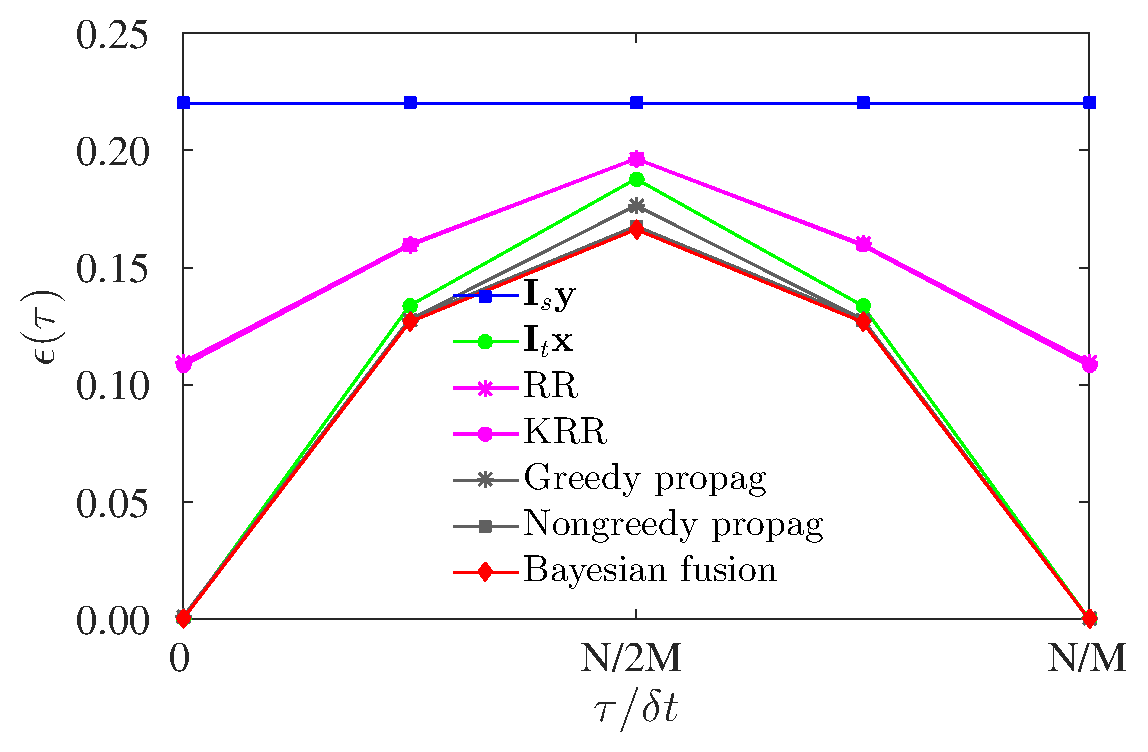
\includegraphics[width = 0.7\columnwidth]{./images/comparisons/isotropic/compare_NRMSE_time_middlepoints_sspacing3_tspacing4.eps}
\caption{\label{fig:final_isotropic_error_time_case5} Isotropic turbulence: NRMSEs are functions of time distances from the previous LTHS instant at the most difficult spatial location, i.e. at $ (\Delta y/2,\Delta z/2,\tau) $. These errors are estimated between reference and reconstructed streamwise velocities by spatial and temporal interpolations, RR, KRR, non-greedy propagation and Bayesian fusion models. Results are shown for case 5 in table \ref{tab:comparisons_various_cases}, with the subsampling ratios $ \dimth/\dimtl = 4 $ in time and $ \dimsh/\dimsl = 3 \times 3 $ in space.}
\end{center}
\end{figure}

\begin{figure}
\begin{center}
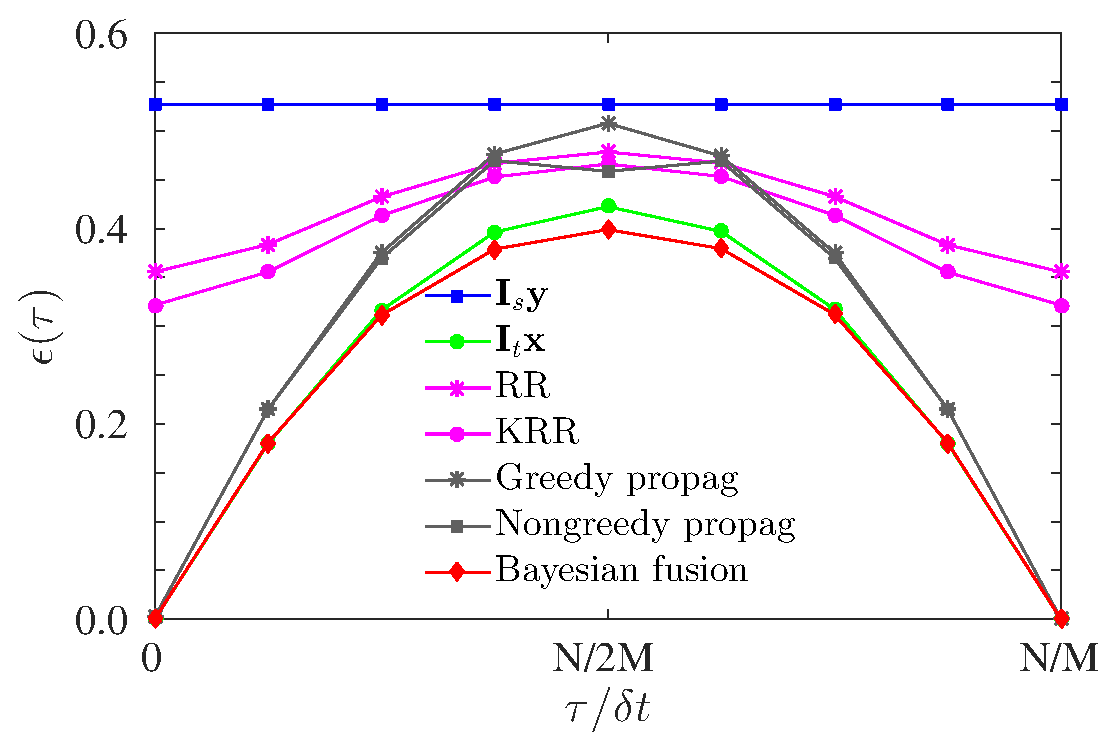
\includegraphics[width = 0.7\columnwidth]{./images/comparisons/isotropic/compare_NRMSE_time_middlepoints_sspacing6_tspacing8.eps}
\caption{\label{fig:final_isotropic_error_time_case7} Isotropic turbulence: similar plot as figure \ref{fig:final_isotropic_error_time_case5} for case 7 in table \ref{tab:comparisons_various_cases}, with the subsampling ratios $ \dimth/\dimtl = 8 $ in time and $ \dimsh/\dimsl = 6 \times 6 $ in space.}
\end{center}
\end{figure}

\begin{figure}[h]
\begin{center}
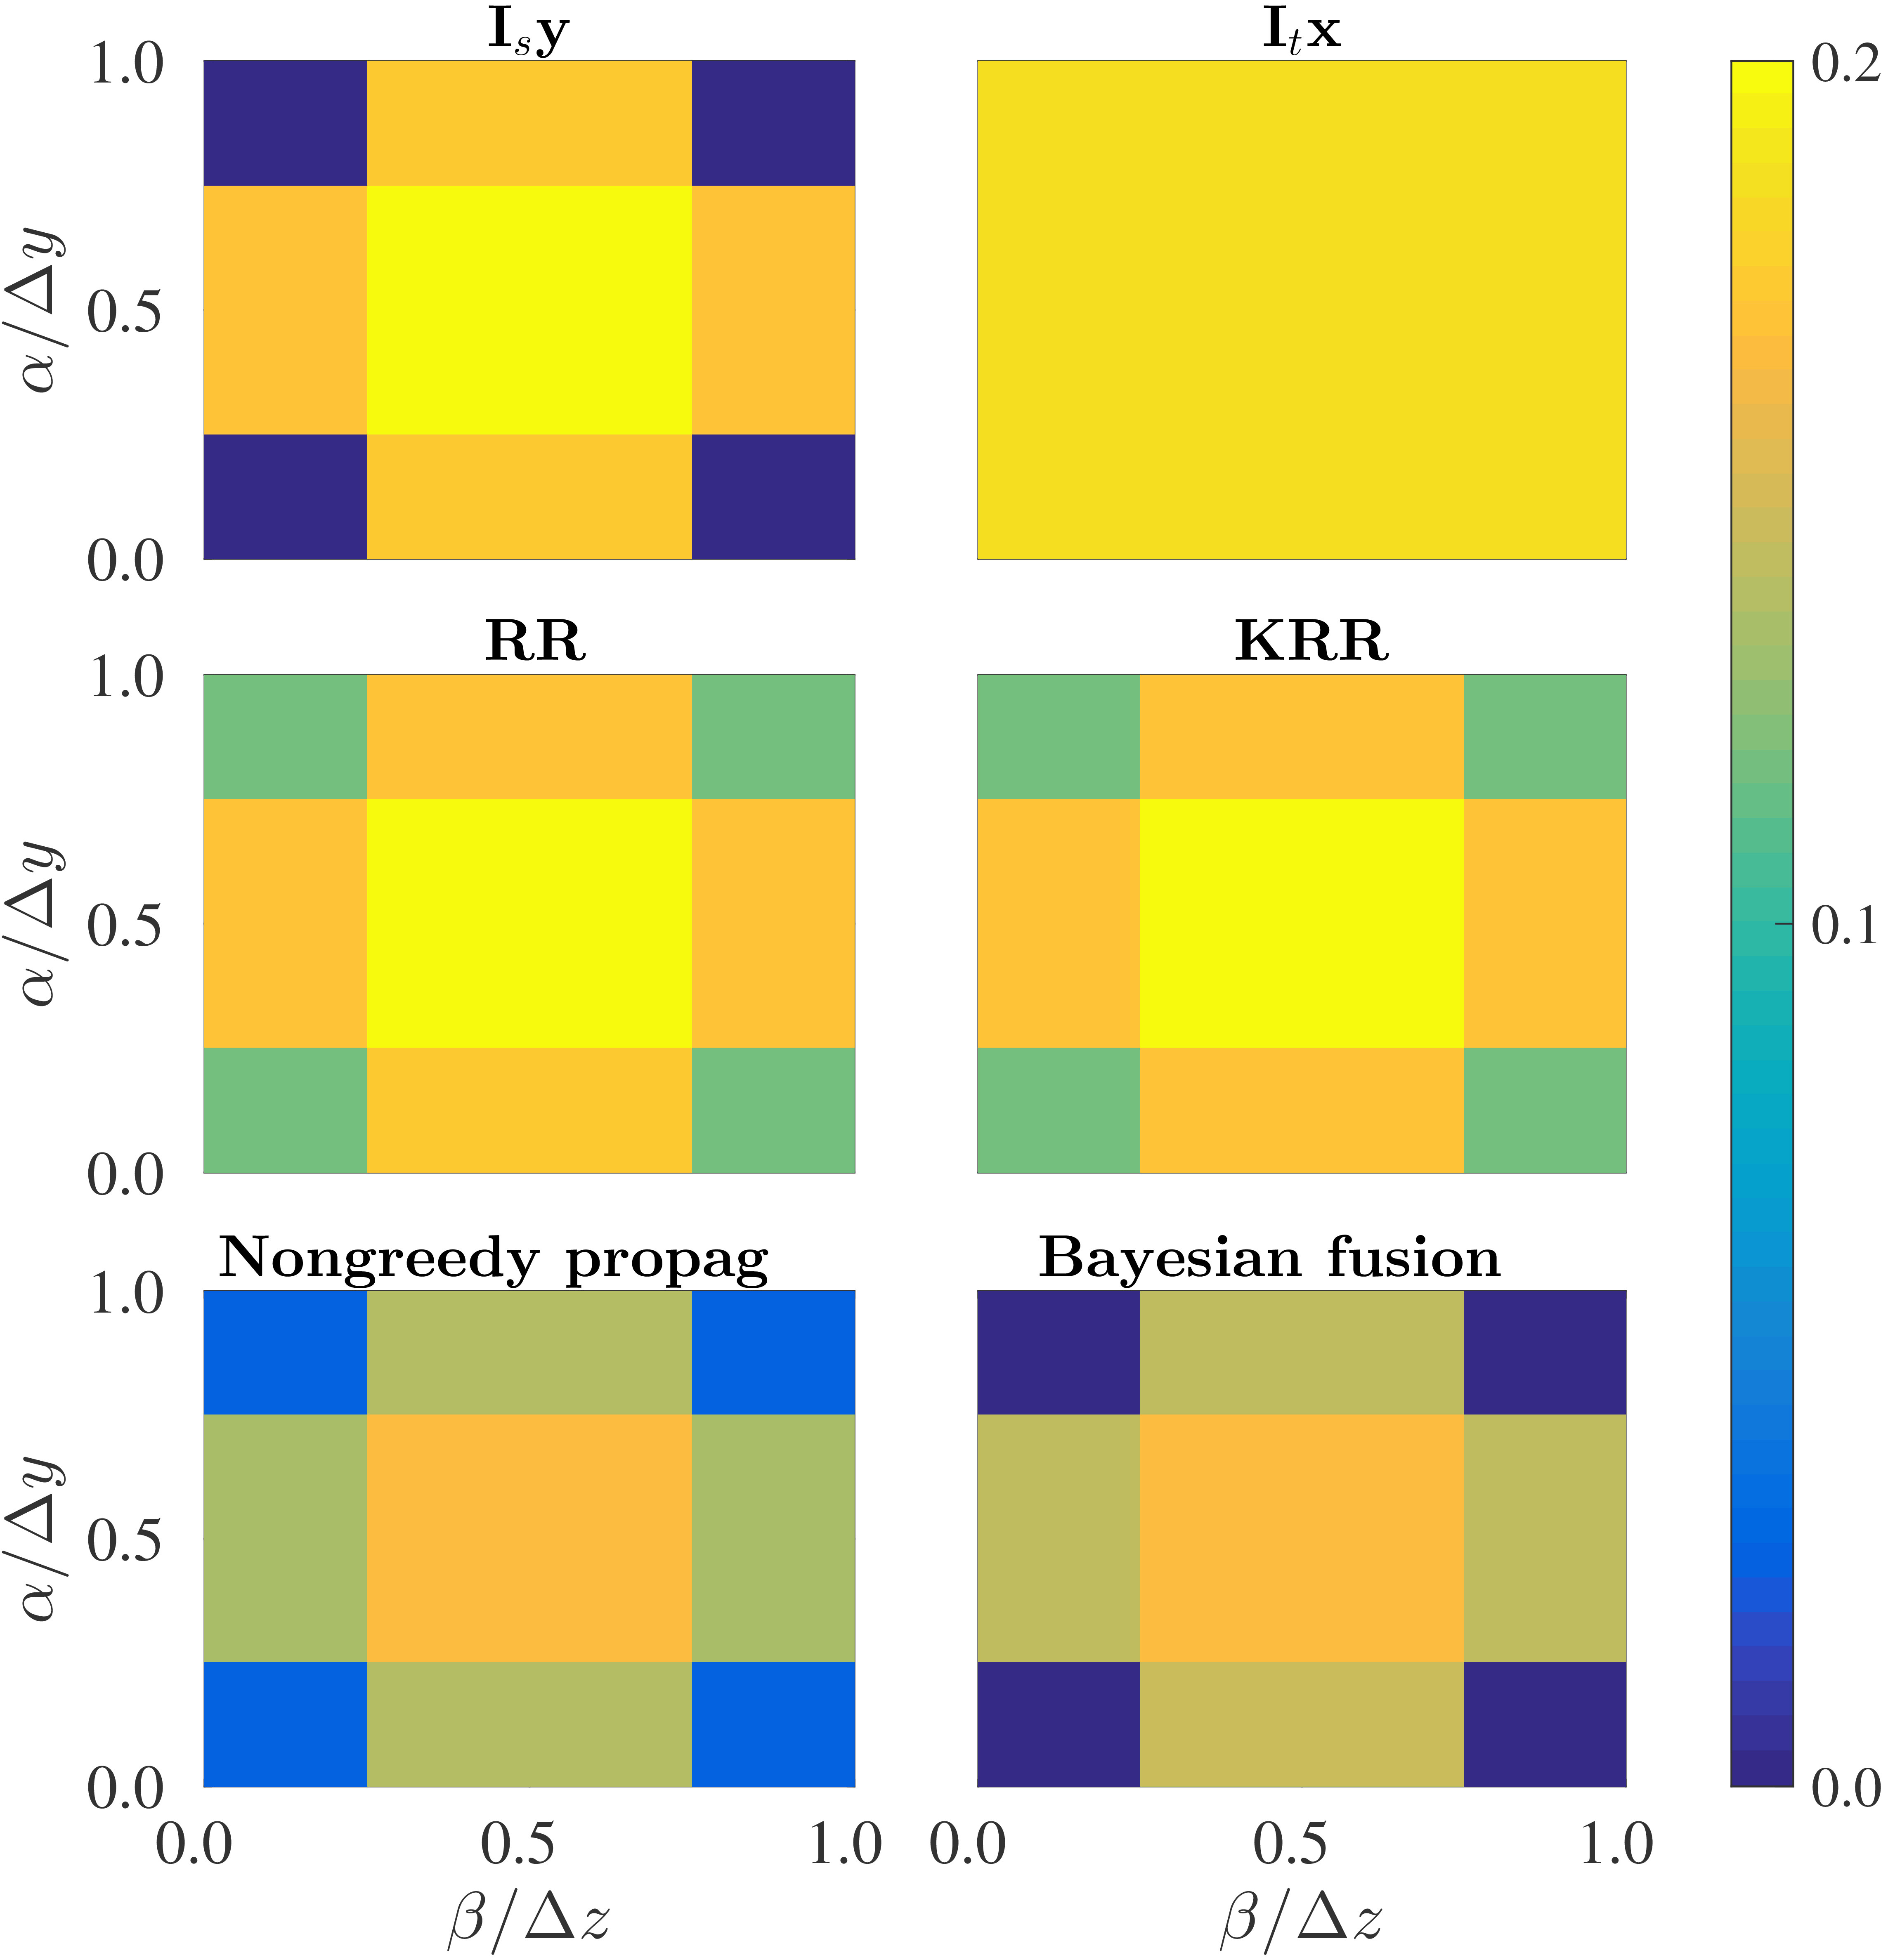
\includegraphics[width = 0.8\columnwidth]{./images/comparisons/isotropic/compare_boxin4HWs_sspacing3_tspacing4.png}
\caption{\label{fig:final_isotropic_error_boxes_case5} Isotropic turbulence: NRMSEs are functions of spatial coordinates in an element block at the most difficult instant, i.e. at $ (\alpha,\beta,\dimth \delta t/2\dimtl) $. These errors are estimated between reference and reconstructed streamwise velocities by spatial and temporal interpolations, RR, KRR, non-greedy propagation and Bayesian fusion models. Results are shown for case 5 in table \ref{tab:comparisons_various_cases}, with subsampling ratios of $ \dimth/\dimtl = 4 $ in time and $ \dimsh/\dimsl = 3 \times 3 $ in space.}
\end{center}
\end{figure}

\begin{figure}[h]
\begin{center}
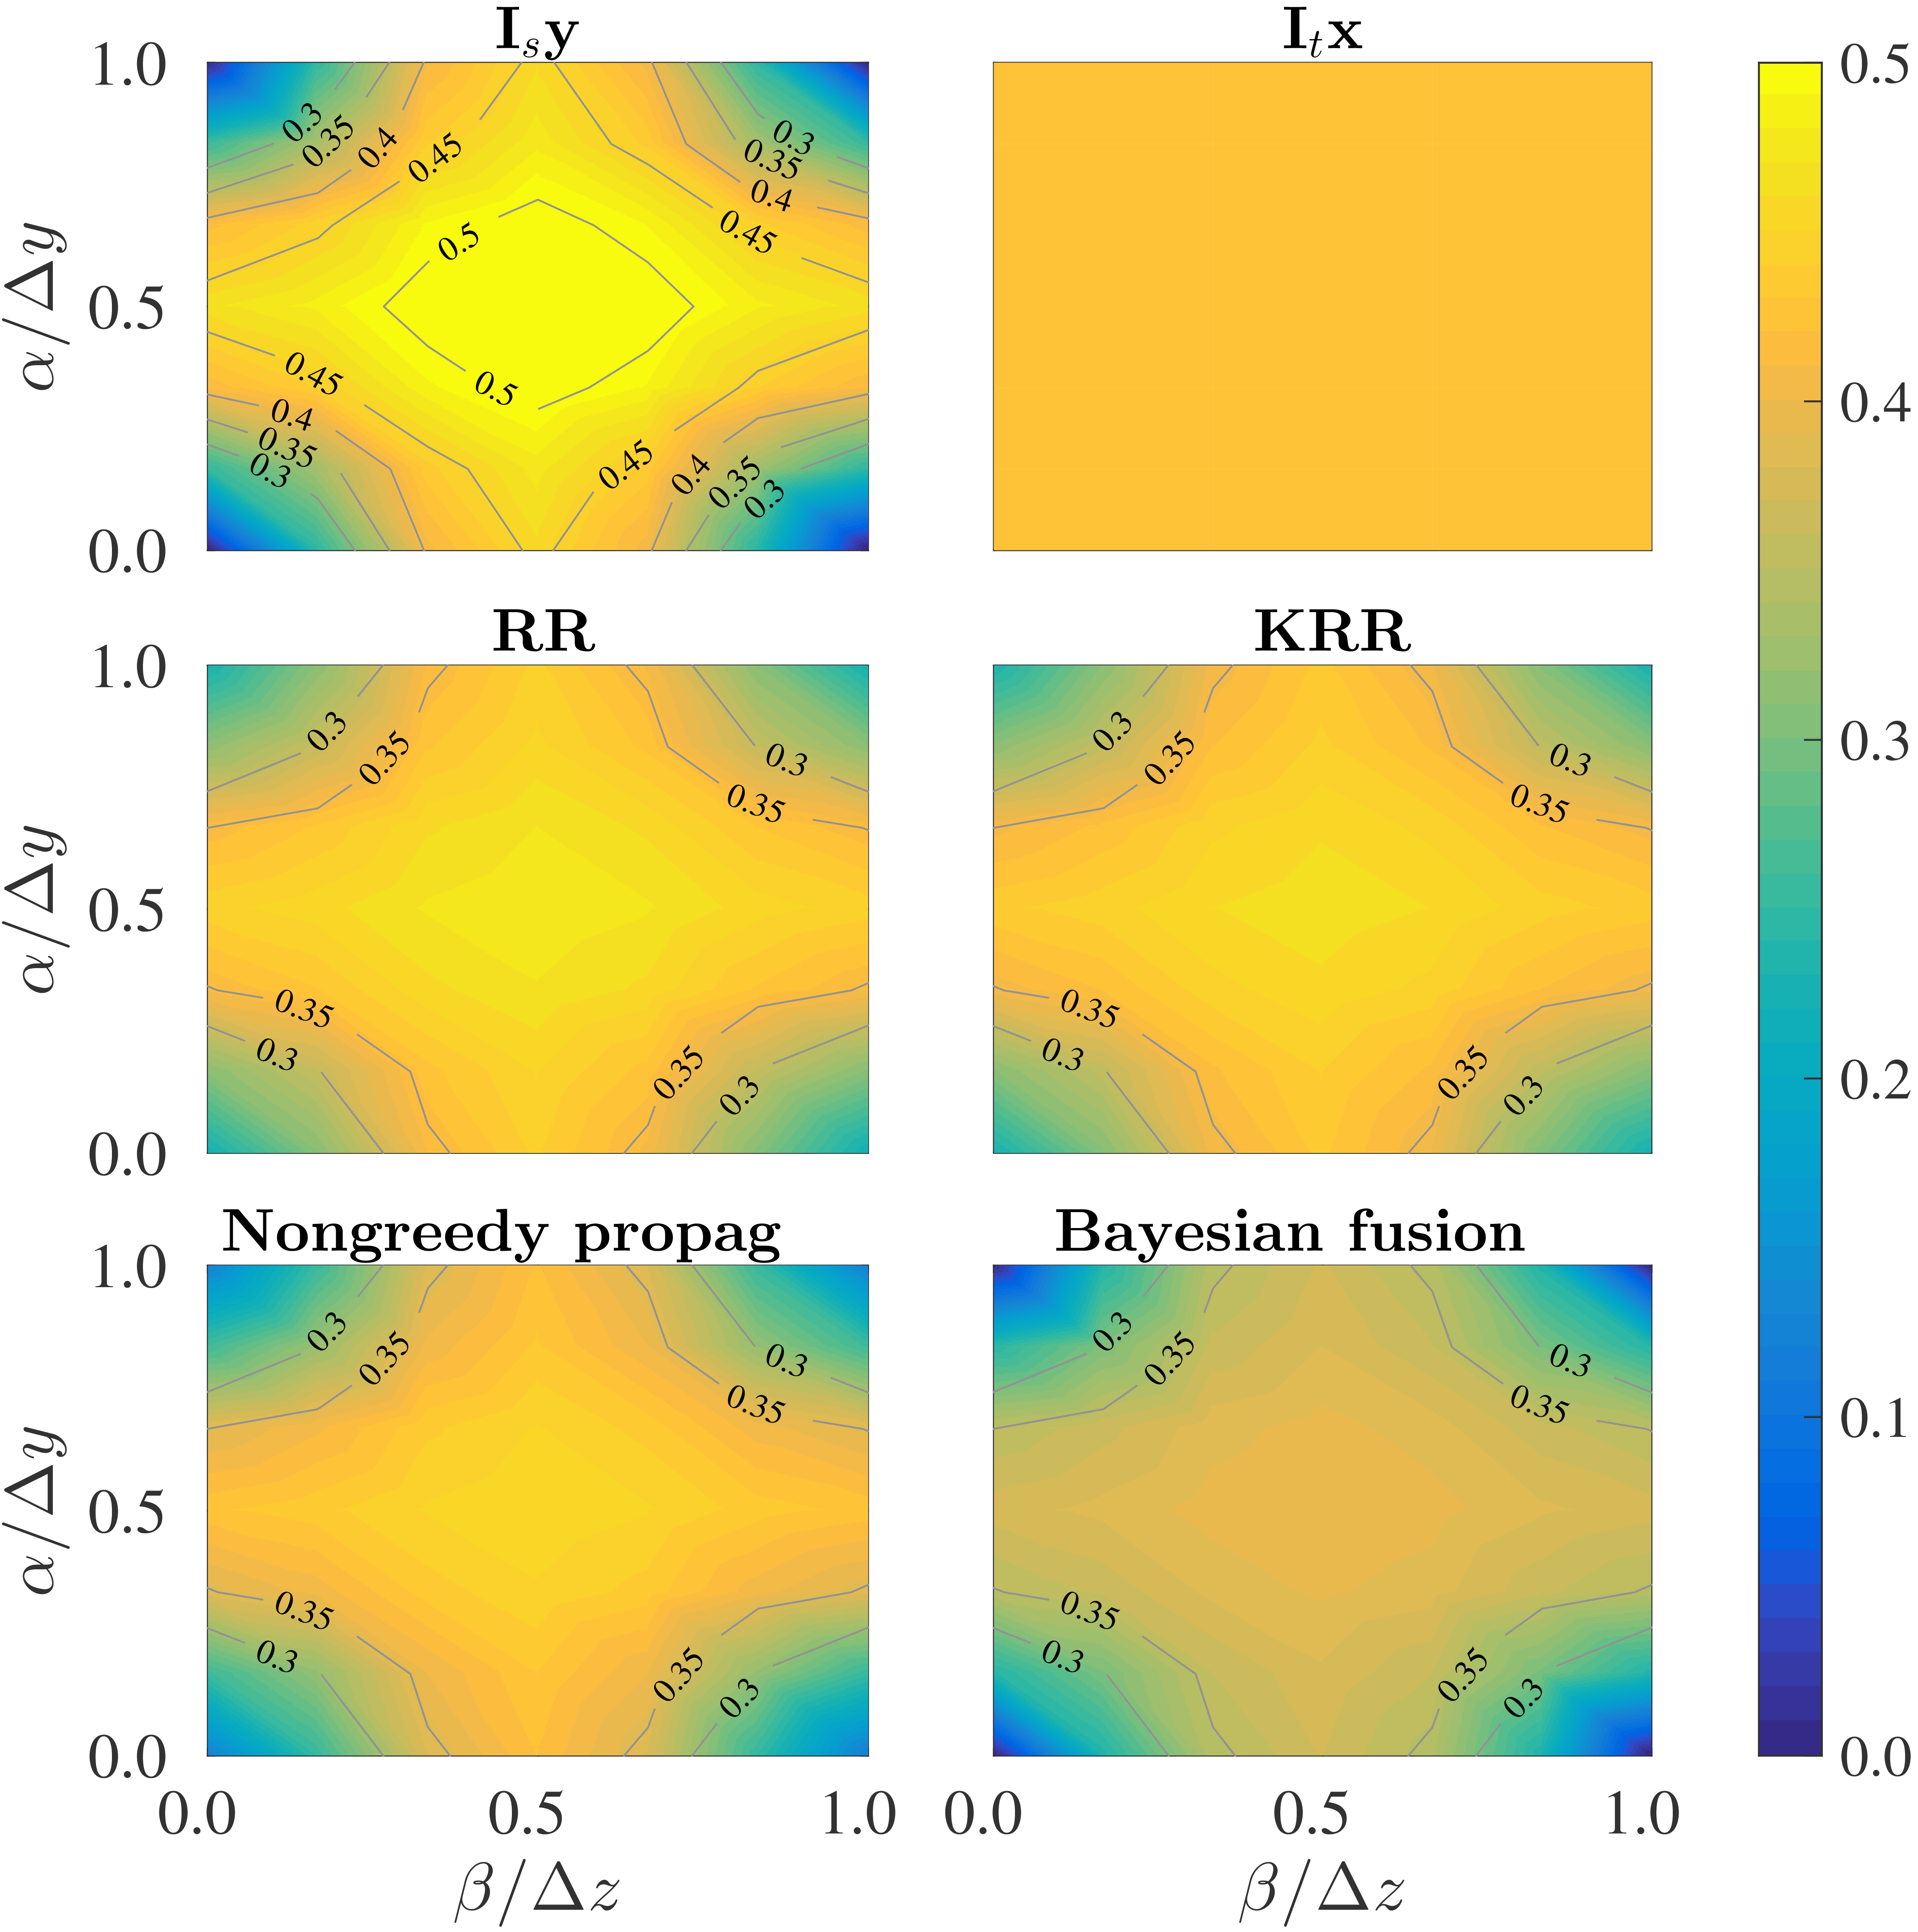
\includegraphics[width = 0.8\columnwidth]{./images/comparisons/isotropic/compare_boxin4HWs_sspacing6_tspacing8.png}
\caption{\label{fig:final_isotropic_error_boxes_case7} Isotropic turbulence: NRMSEs are functions of spatial coordinates as in figure \ref{fig:final_isotropic_error_boxes_case5}. Results are shown for case 7 in table \ref{tab:comparisons_various_cases}, with subsampling ratios of $ \dimth/\dimtl = 8 $ in time and $ \dimsh/\dimsl = 6 \times 6 $ in space.}
\end{center}
\end{figure}

To analyze the reconstructions in time, figure \ref{fig:final_isotropic_error_time_case5} shows NRMSEs as a function of distances $ \tau $ from the previous LTHS time step in cases 5. For each $ \tau $, NRMSE is estimated using the set of point $ \varmathbb{J}$ including points at local coordinates $ (\Delta y/2,\Delta z/2, \tau) $ of all blocks used to estimate $ \epsilon_{max} $. NRMSEs are small close to the LTHS measurements ($ \tau/\delta t=0 $ and $ \tau/\delta t=\dimth/\dimtl $) and increase when moving toward the middle ($ \tau/\delta t=\dimth/2\dimtl $). Spatial interpolation behaves differently since the NRMSE is independent of time. Regression models illustrate the advantages of learning a model by significantly reducing the errors (about $ 15 \% $ for mid-planes at $ \dimth/\dimtl $) compared to spatial interpolation. Time interpolation gives smaller error than RR and KRR, since those errors of regression models depend only on the subsampling ratio in space. These temporal information from LTHS planes are taken into account to further improve the reconstruction using fusion models. Both the propagation models and fusion model give better reconstructions than all other models. Bayesian fusion and non-greedy model are slightly better than the greedy one.

Figure \ref{fig:final_isotropic_error_time_case7} shows similar results as in figure \ref{fig:final_isotropic_error_time_case5} for case 7 with very severe subsampling ratios in both space and time. Model performances are consistent with case 5, except that propagation models now give higher NRMSEs than time interpolation. This is because the propagation models start from a critical loss of information and could not recover completely. Also, this approach does not take advantages of temporal information from LTHS snapshots (except their small scales to propagate). Bayesian fusion model, which proposes a compromise estimate between the two interpolations. The model yields the minimum errors at all time steps. Even in the middle of two LTHS instants, the maximum fusion error remains lower than the one obtained with both interpolations. 

To analyze the reconstructions in space, figures \ref{fig:final_isotropic_error_boxes_case5} and \ref{fig:final_isotropic_error_boxes_case7} show spatial NRMSE maps by all the methods as a function of local coordinates $ (\alpha,\beta) $ as described in figure \ref{fig:element_block}, section \ref{sec:probdef2}. For each $ (\alpha,\beta) $, NRMSE is estimated using equation~(\ref{eq:NRMSE}), where $ \varmathbb{J} $ includes points at $ (\alpha,\beta,\dimth \delta t/2 \dimtl) $ of all blocks used to estimate $ \epsilon_{max} $. All methods give small NRMSEs close to the four HTLS positions in the corners. The errors increase when approaching the center. Time interpolation behaves differently since the errors are independent of spatial coordinates. Compared to interpolation in space, regression models do not give exact estimates at the HTLS positions. However, errors far from these four points are significantly reduced. The fusion models yields the best reconstruction results, where the Bayesian fusion model yields the smallest errors at all positions. At the most difficult positions (near the center of the block), it improves the reconstruction significantly compared to other methods. 


\begin{figure}
\begin{center}
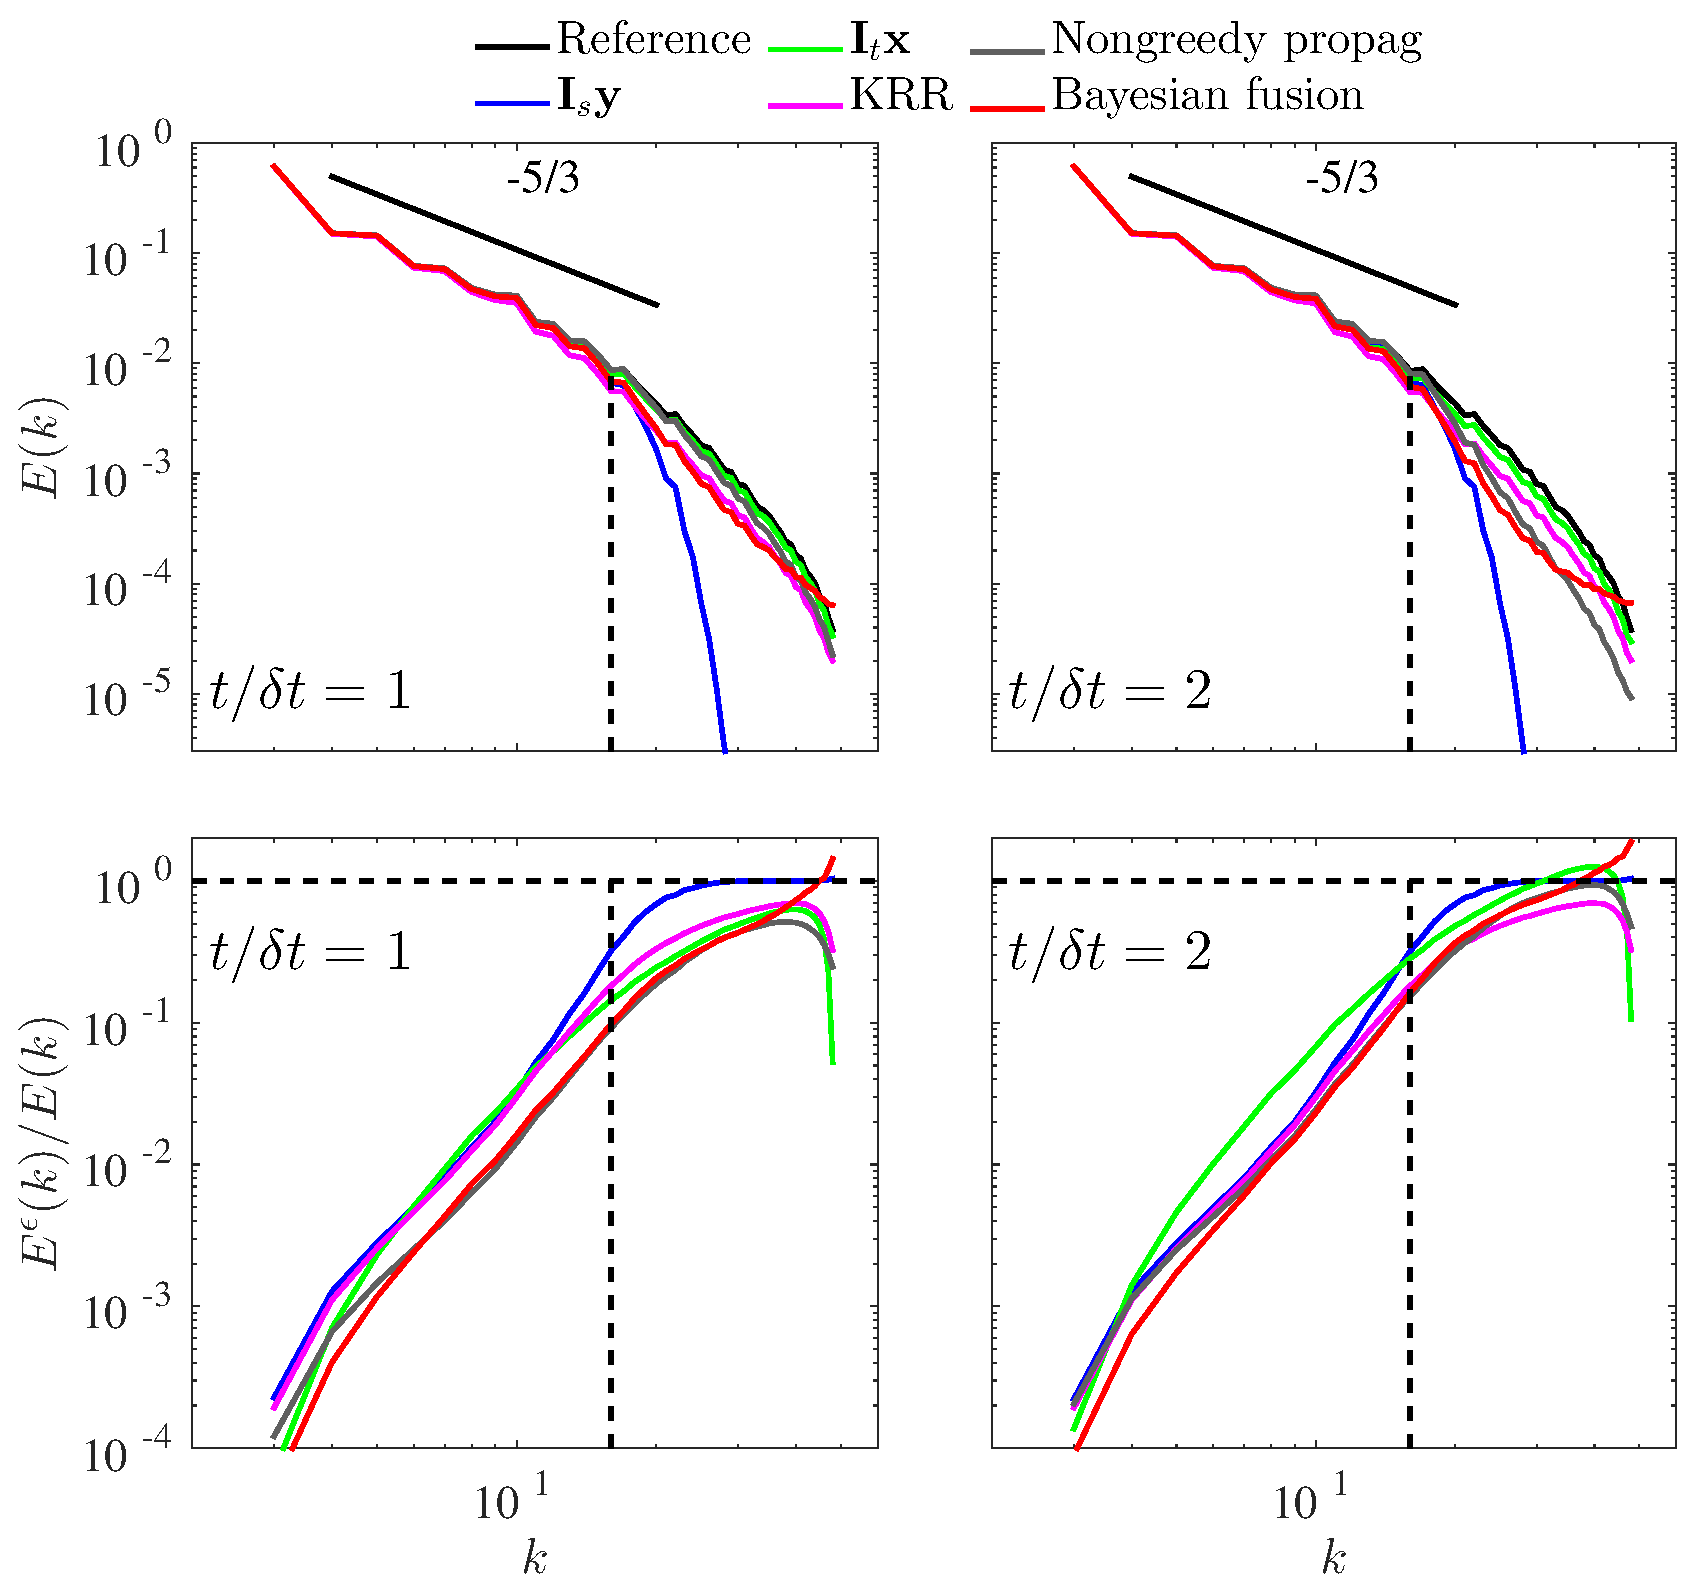
\includegraphics[width = 0.8\columnwidth]{./images/comparisons/isotropic/spectra_sspacing3_tspacing4.eps}
\caption{\label{fig:spectra_sspacing3_tspacing4} Isotropic turbulence: comparison of energy spectra and error spectra for reconstructions by interpolations (in space and time), KRR, non-greed propagation and Bayesian fusion model in case 5 of subsampling ratios $ \dimsh/\dimsl = 3 \times 3 $ in space and $ \dimth/\dimtl = 4 $ in time (see table \ref{tab:comparisons_various_cases}). The spectra are averaged over all planes of the same distance to the closest LTHS plane, i.e. $ t/\delta t = 1 $ (left) or $ t/\delta t = 2 $ (right).}
\end{center}
\end{figure}

Figure \ref{fig:spectra_sspacing3_tspacing4} shows the spectral analysis of the reconstruction by different models. To make the plot readable, RR, greedy propagation and linear Gaussian models are omitted. Energy spectra and error spectra are shown for the two positions, either close or far from LTHS planes. The first two spectra illustrate that spatial interpolation captures only large-scale information, while time interpolation gives an estimate with a good energy spectrum. All models are subject to a certain energy loss at small scales. The error spectra shows that time interpolation gives good energy spectra with poorly reconstructed small scales. KRR also shows significant improvement compared to spatial interpolation, both in energy spectra and error spectra. Compared to those that have been shown in figure \ref{fig:NLmean_interps_sspacing3_tspacing4_spectra2d}, the Bayesian fusion model Bayesian fusion model shows similar results compared to the non-greedy propagation. Both models yield compromise estimates, where certain amount of small scales are captured. Error spectra illustrate improvements at all frequencies compared to both interpolations.

\section{Reconstruction results on DNS data of channel flow}
\label{sec:comparisons_channel}
This section further analyses and compares performances of proposed methods on the DNS data of a turbulent channel flow with a moderate Reynolds number as described in section \ref{sec:data_channel}. This data mimics the experiments from WALLTURB project \citep{coudert2011double}, and simulates better practical flows compared to isotropic turbulence. Its characteristics are strongly non-homogeneous in vertical direction. The real ``time'' dimension is considered instead of a ``virtual'' one as in the previous dataset.

\begin{table}[t]
	\caption{\label{tab:final_various_cases_channel}
	Channel flow: configuration parameters of seven testing cases. The subsampling ratios of HTLS measurements are $ \sqrt{N/M} $ and equal in both spatial directions. The ratios of LTHS measurements in time are $ P/Q $. The spacing in spanwise direction is normalized by half channel height as $ \Delta z/H $ and the spacing in time is $\Delta t$, normalized by $ H/U_{max} $ ($ U_{max} $ is the central velocity of the flow). The normalized energy losses in space $\Delta\kappa_s$ and in time $\Delta\kappa_t$ are defined in Eq.~(\ref{eq:RMS_losses}).}
	\vspace{.5cm}
	\centering
	\begin{tabular}{ccS[table-format=2.0]S[table-format=2.0]cS[table-format=1.2]S[table-format=1.2]cS[table-format=1.2]S[table-format=2.2]} 
		\toprule
		\multirow{2}{*}{Case}&\multicolumn{1}{c}{}&\multicolumn{2}{c}{Subsampling ratios}&\multicolumn{1}{c}{}&\multicolumn{2}{c}{Spacings}&\multicolumn{1}{c}{}&\multicolumn{2}{c}{Energy loss}\\ 
		\cmidrule{3-4} \cmidrule{6-7} \cmidrule{9-10}
		 & & {$\sqrt{\dimsh/\dimsl}$} & $\dimth/\dimtl$ & & {$\Delta z/H$} & {$\Delta t$} & & {$\Delta\kappa_s(\%)$} & {$\Delta\kappa_t (\%)$}\\ 
		\midrule 
		5 &  & 05  & 04 & & 0.05  & 0.10 & & 1.23 & 1.88 \\ %\addlinespace	 
		6 &  & 10  & 10 & & 0.11  & 0.25 & & 7.08 & 9.02 \\ %\addlinespace
		7 &  & 20  & 20 & & 0.22  & 0.50 & & 20.83 & 24.31\\ %\addlinespace
		\bottomrule
	\end{tabular}
\end{table}


\begin{table}
\caption{\label{tab:final_results_channel}
Channel flow: NRMSEs of all scales reconstruction errors for three cases in Table.~\ref{tab:final_various_cases_channel}. $\overline{\epsilon}$ and $\epsilon_{max}$ are the mean and max NRMSE defined in Eq.~(\ref{eq:NRMSE}). $\overline{\epsilon}$ is averaged over all space-time positions in the outer region $ y/H \in [0.25,1.75] $, while $\epsilon_{max}$ is computed for one of the most difficult position in space and time (the most remote from all nearby measurements). The smallest errors in each cases are boldfaced.}
\vspace{.5cm}
\centering
	\begin{tabular}{lcccccccc} 
		\toprule \multirow{2}{*}{Method}&\multicolumn{1}{c}{}&\multicolumn{3}{c}{$\overline{\epsilon}$}&\multicolumn{1}{c}{}&\multicolumn{3}{c}{$\epsilon_{max}$}\\
		\cmidrule{3-5} \cmidrule{7-9}
		 & & {Case 5} & {Case 6} & {Case 7} & & {Case 5} & {Case 6} & {Case 7}\\
		\midrule 
		$ \Interp_s \y $ & & 0.14 & 0.36 & 0.68 & & 0.16 & 0.47 &  0.85 \\ 
		$ \Interp_t \x $ & & 0.11 & 0.32 & 0.54 & & 0.18 & 0.55 &  0.85 \\
		RR & & 0.12 & 0.34 & 0.64 & & 0.15 & 0.49 &  0.78 \\
    	Fusion (BF)  & & 0.08 & 0.25 & 0.46 & & 0.13 &  0.43 &  0.73 \\ 
    	\midrule
    	\myrowcolour
    	Best scores  & & \textbf{0.08} & \textbf{0.25} & \textbf{0.46} & & \textbf{0.13} &  \textbf{0.43} &  \textbf{0.73} \\ \bottomrule
	\end{tabular}
\end{table}

Based on the analyses on isotropic turbulence, and for simplicity, only RR and Bayesian fusion model are selected to represent the two families of approaches. Three cases of balanced subsamplings in space and time are considered. The configurations with subsampling ratios, spacings and amounts of energy loss are presented in table \ref{tab:final_various_cases_channel}. The losses in space (2D) and time are similar in each case, from very small energy losses (less than $ 1 \sim 2 \% $ in case 5) to very severe ones (more than $ 20 \% $ in case 7). The average and maximum NRMSEs of reconstructions by all methods for the three cases are shown in table \ref{tab:final_results_channel}. The best errors obtained by the fusion model are boldfaced and shown in the last row. 


\begin{figure}
\begin{center}
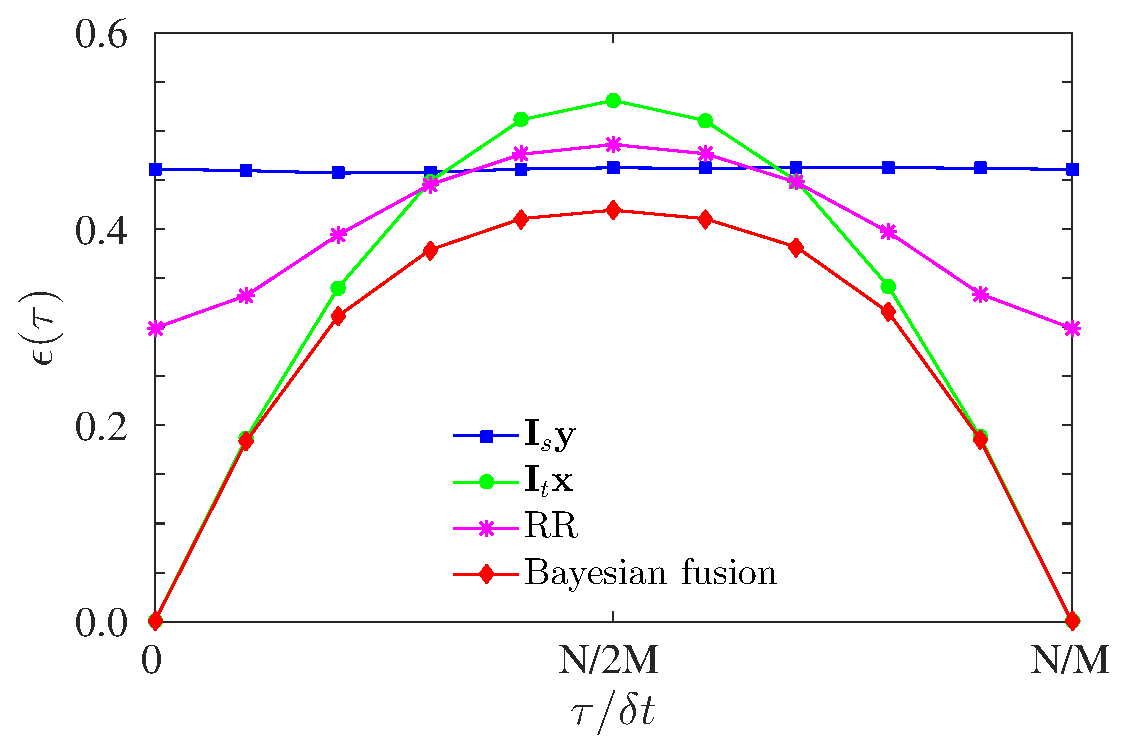
\includegraphics[width = 0.8\columnwidth]{./images/comparisons/channel/error_MAP_newOM1_middlepoint_outer.eps}
\caption{\label{fig:final_channel_error_time} Channel flow: NRMSEs between reference and reconstructed streamwise velocities by all methods as: functions of time distances from the previous LTHS instant at the most difficult spatial location, i.e. at $ (\Delta y/2,\Delta z/2,\tau) $. Results are shown for case 5 in table \ref{tab:final_various_cases_channel}, with the subsampling ratios $ \dimth/\dimtl = 10 $ in time and $ \dimsh/\dimsl = 10 \times 10 $ in space.}
\end{center}
\end{figure}

\begin{figure}
\begin{center}
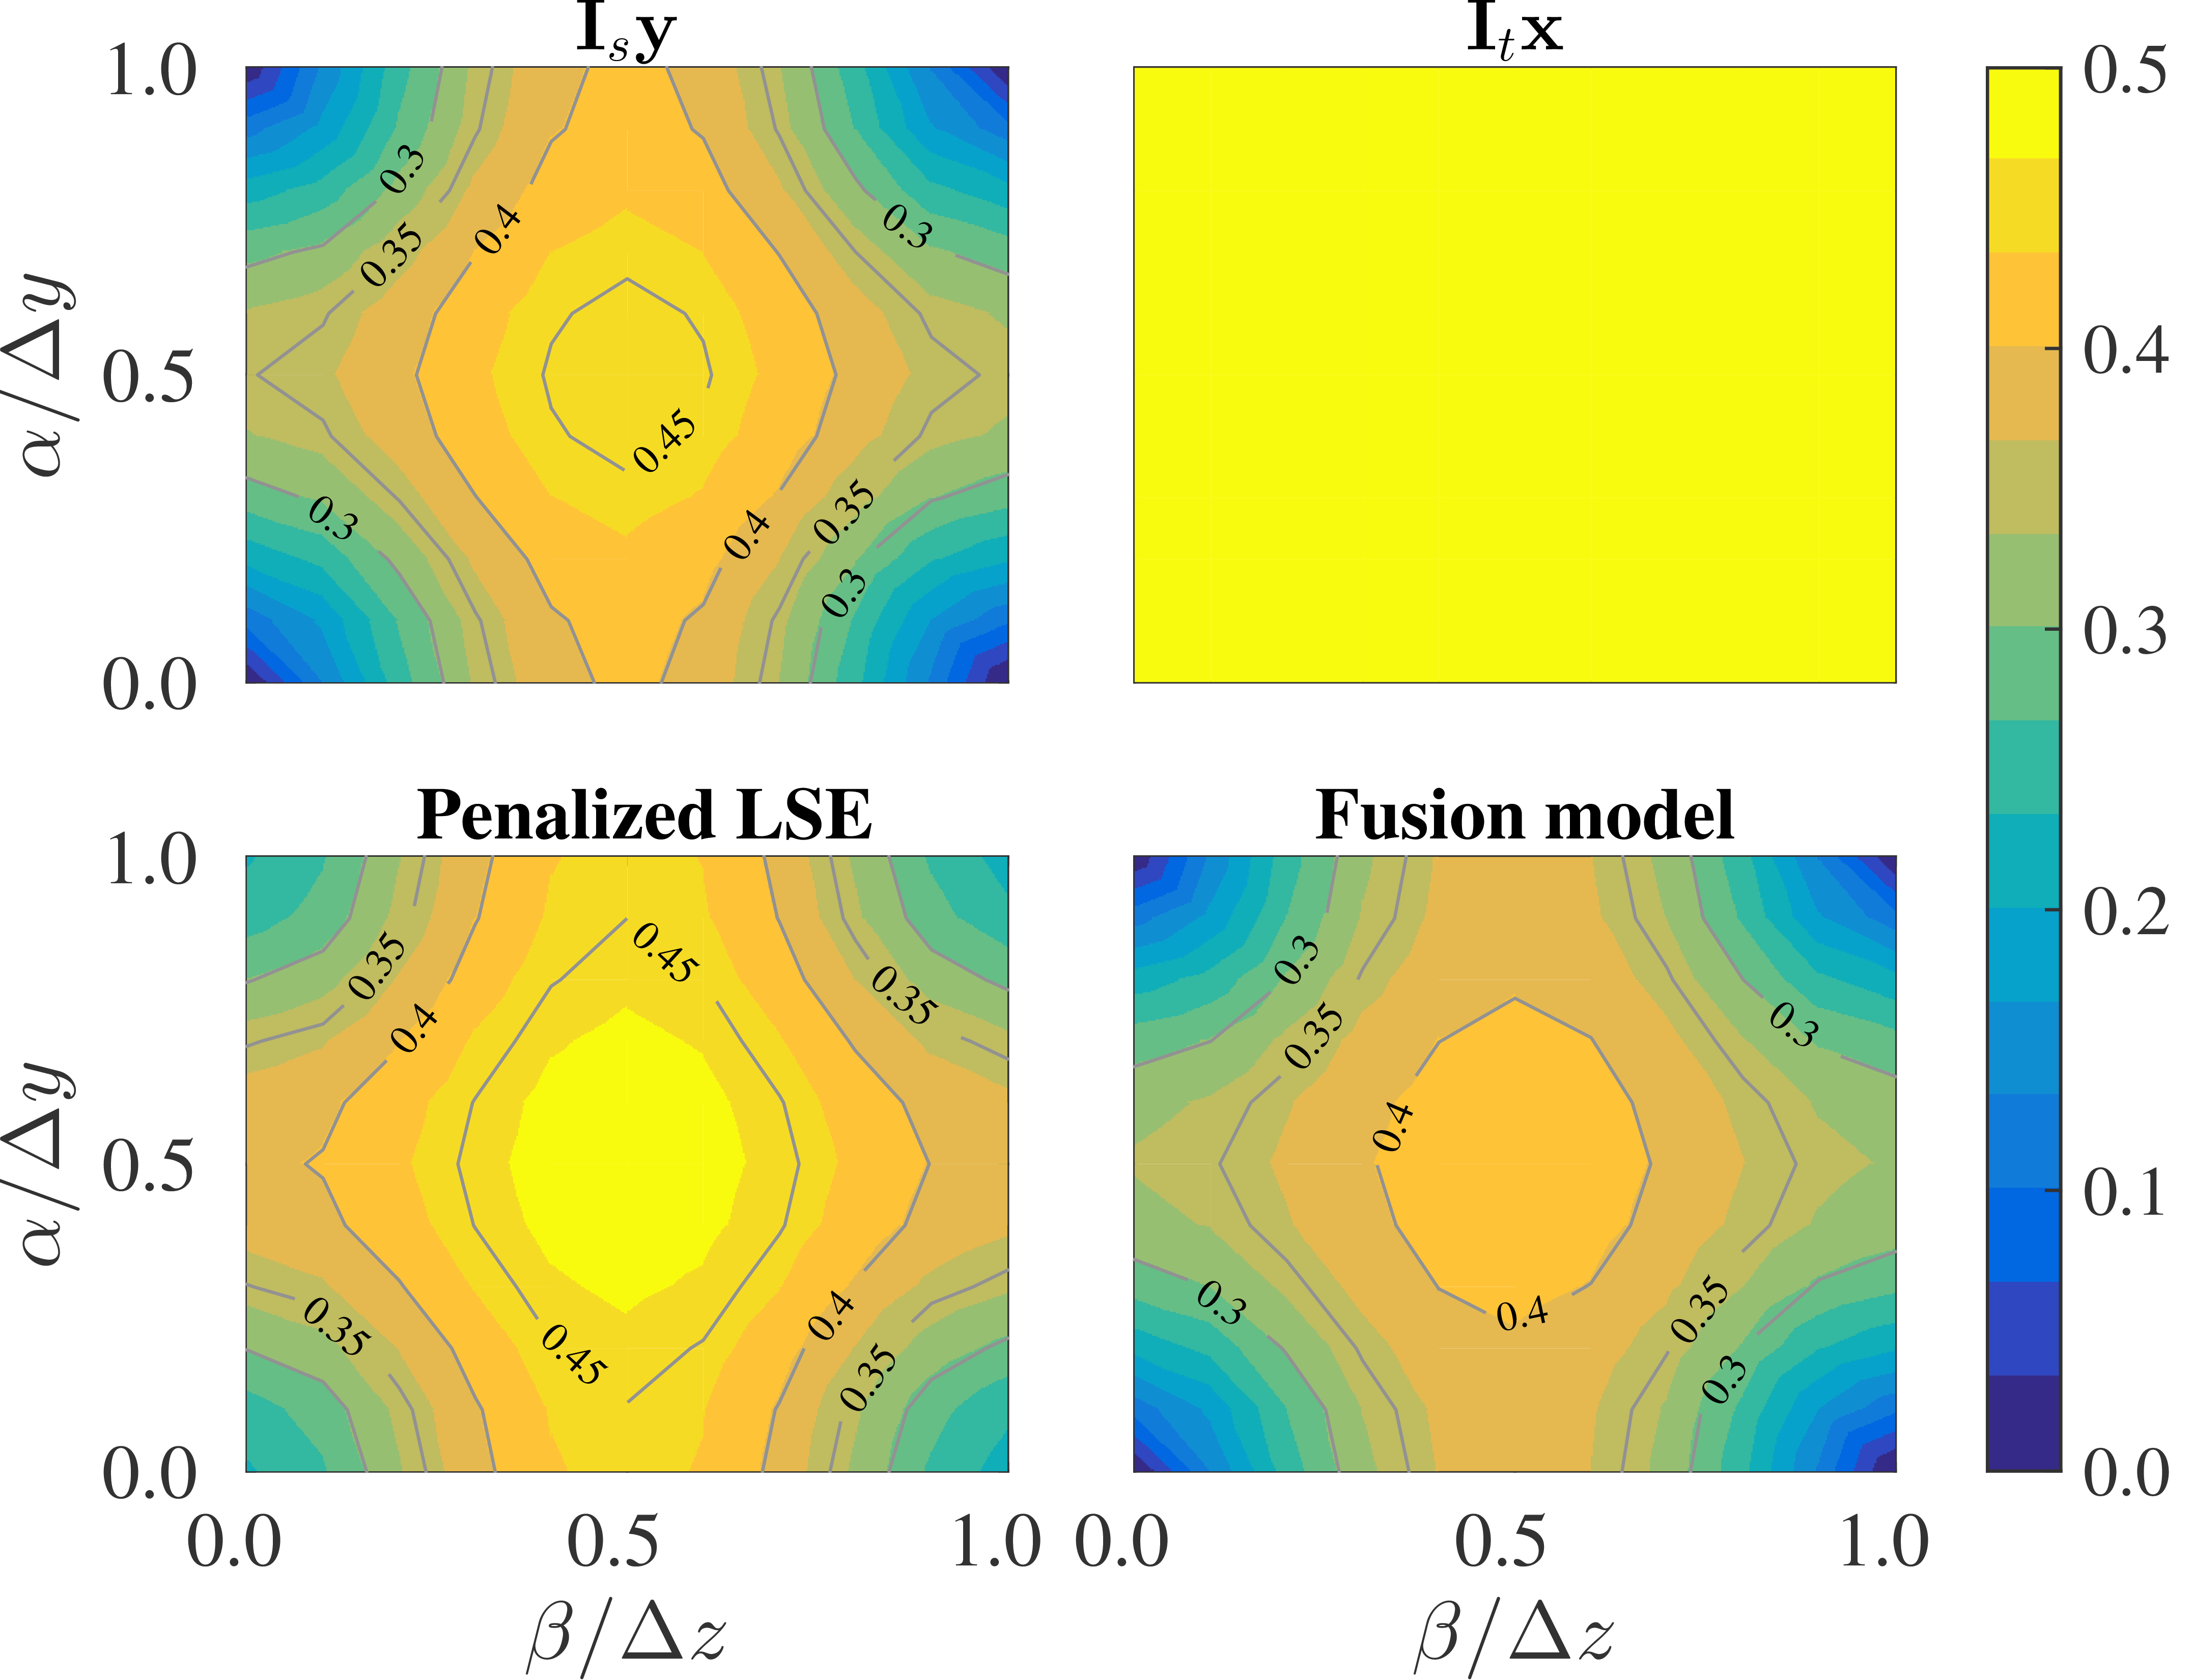
\includegraphics[width = 0.8\columnwidth]{./images/comparisons/channel/error_MAP_newOM1_boxin4HWs_outer.png}
\caption{\label{fig:final_channel_error_boxes} Channel flow: NRMSEs between reference and reconstructed streamwise velocities by all methods as: functions of spatial coordinates in an element block at the most difficult instant, i.e. at $ (\alpha,\beta,\dimth \delta t/2\dimtl) $. Results are shown for case 5 in table \ref{tab:final_various_cases_channel}, with the subsampling ratios $ \dimth/\dimtl = 10 $ in time and $ \dimsh/\dimsl = 10 \times 10 $ in space.}
\end{center}
\end{figure}



Case 6 of moderate energy loss (about $ 8 \% $) is used for further visualization of the analysis. The energy losses are not too severe but are critical to highlight interests of the present approach. $ \overline{\epsilon} $  and $ \epsilon_{max} $ are reduced by 25 $ \% $ and 35 $ \% $ respectively for all scales reconstruction. Model performances in time and in space are shown in figures \ref{fig:final_channel_error_time} and  \ref{fig:final_channel_error_boxes}respectively. They are estimated and plotted similarly as in figures \ref{fig:final_isotropic_error_boxes_case7} and \ref{fig:final_isotropic_error_time_case5}. The fusion model clearly demonstrates the benefits of combining information in space and time by proposing a compromise estimate from the two single interpolations. 


\begin{figure}
\begin{center}
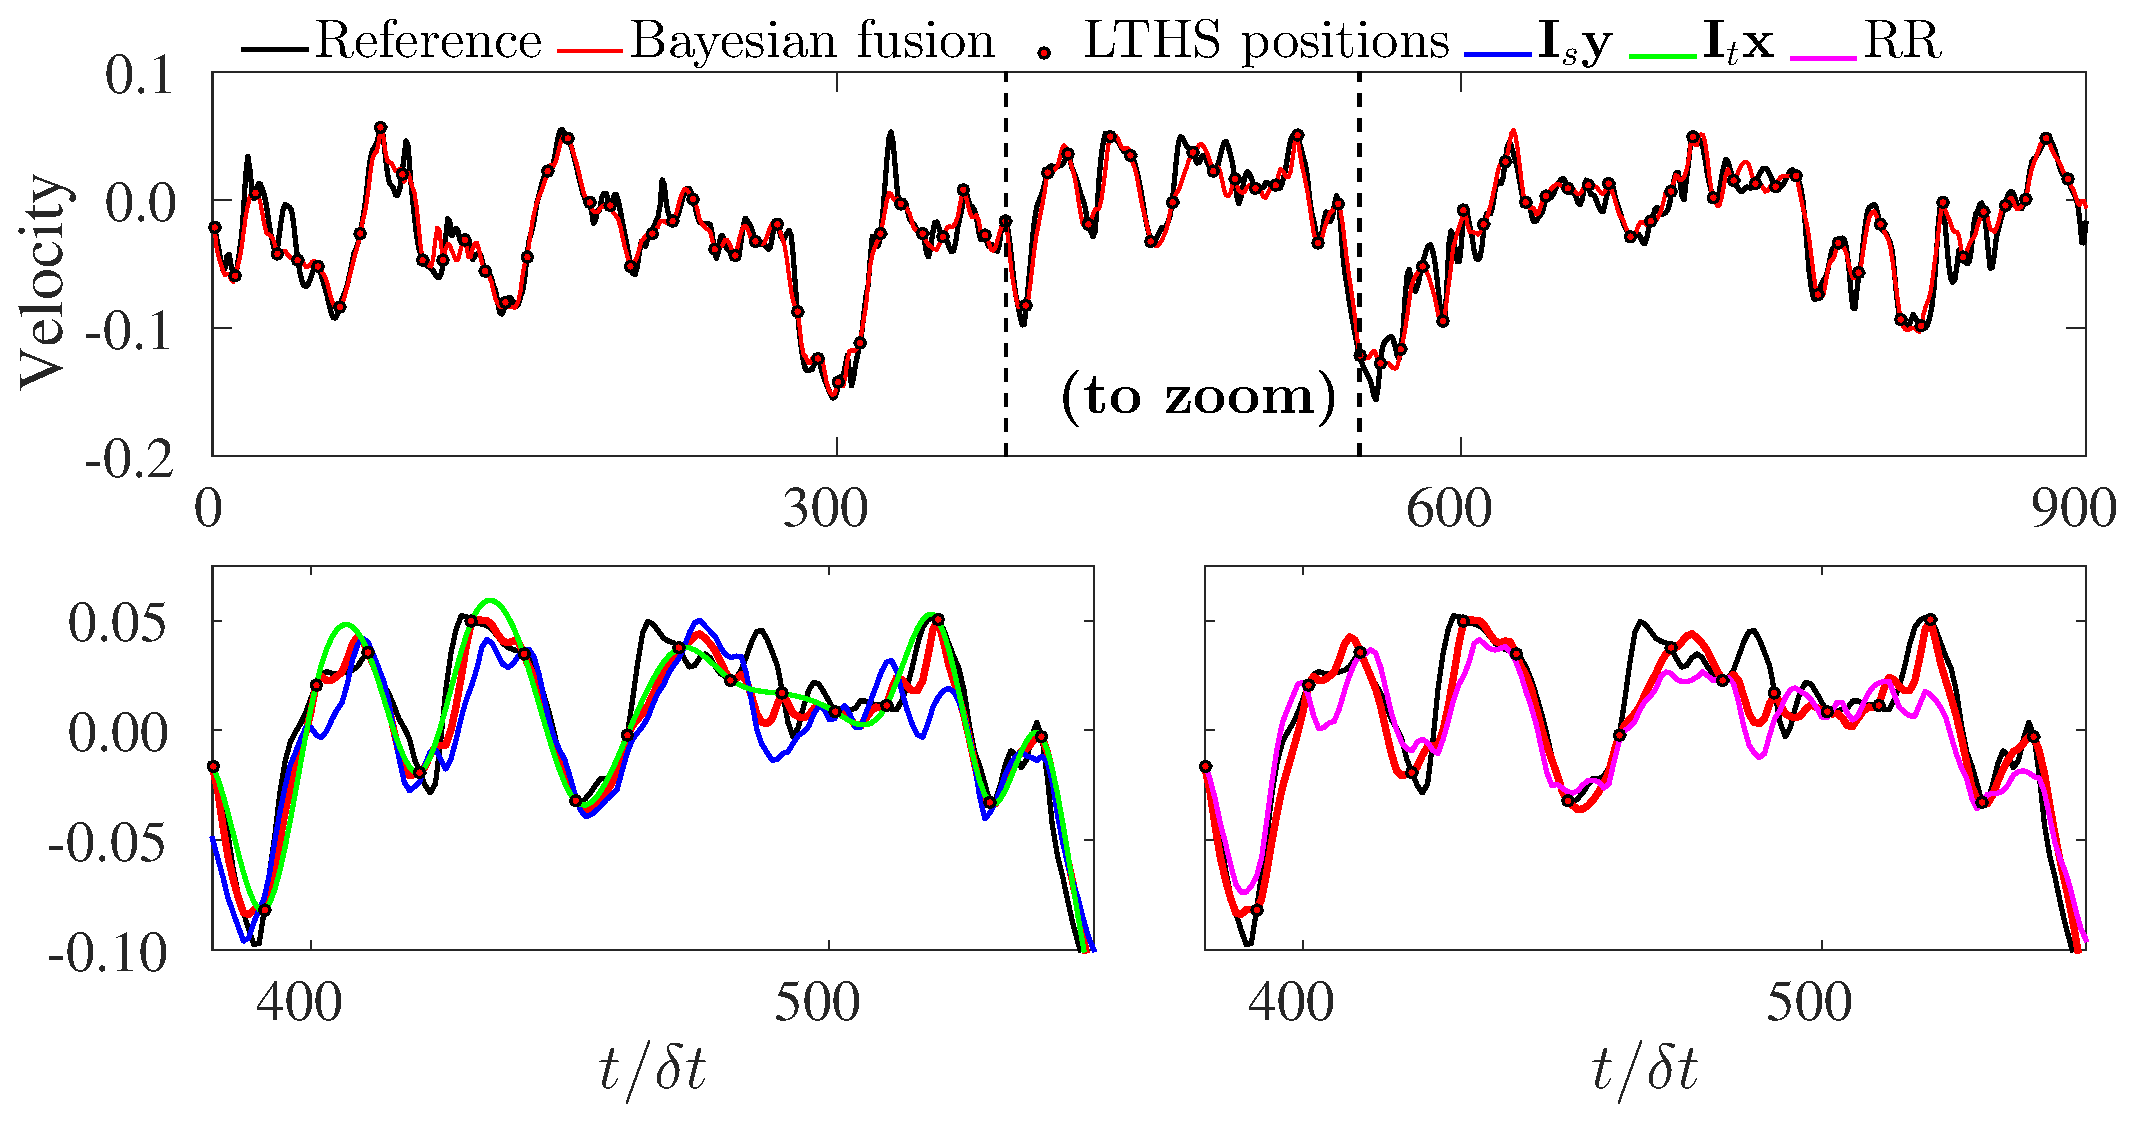
\includegraphics[width=\columnwidth]{./images/comparisons/channel/improper_point_spacespacing_10_timespacing_10_yid129_zid149.eps}
\caption{\label{fig:final_channel_timeseries} Channel flow: a time evolution of fluctuating streamwise velocity at $ y/H=1 $ and $ z/H=0 $ of a point with the local coordinate $ (\Delta y,\Delta z, \tau) $  (see figure (\ref{fig:element_block}) ). The whole evolutions of reference and fused velocity contain $ 900 $ samples. A region is zoomed in and compared with results from interpolations and RR.}
\end{center}
\end{figure}

Figure \ref{fig:final_channel_timeseries} shows a time evolution of the point at $ y/H=1 $ and $ z/H=0 $ ($ \alpha=\Delta y /2 $ and $ \beta = \Delta z/2 $ in local coordinates, see figure \ref{fig:element_block}), the most remote from neighboring HTLS sensors. A good agreement between fused and reference velocity is still obtained. A zoom-in period is shown for detailed comparisons with other methods. While time interpolation captures only low frequencies, spatial interpolation generates high frequencies but weakly correlated with the truth. The fusion model proposes a good compromise to improve both large and small scales reconstruction. It also captures detailed peaks much better than RR, since RR smooths these small scales out by minimizing the mean square errors. 

\begin{figure}
\begin{center}
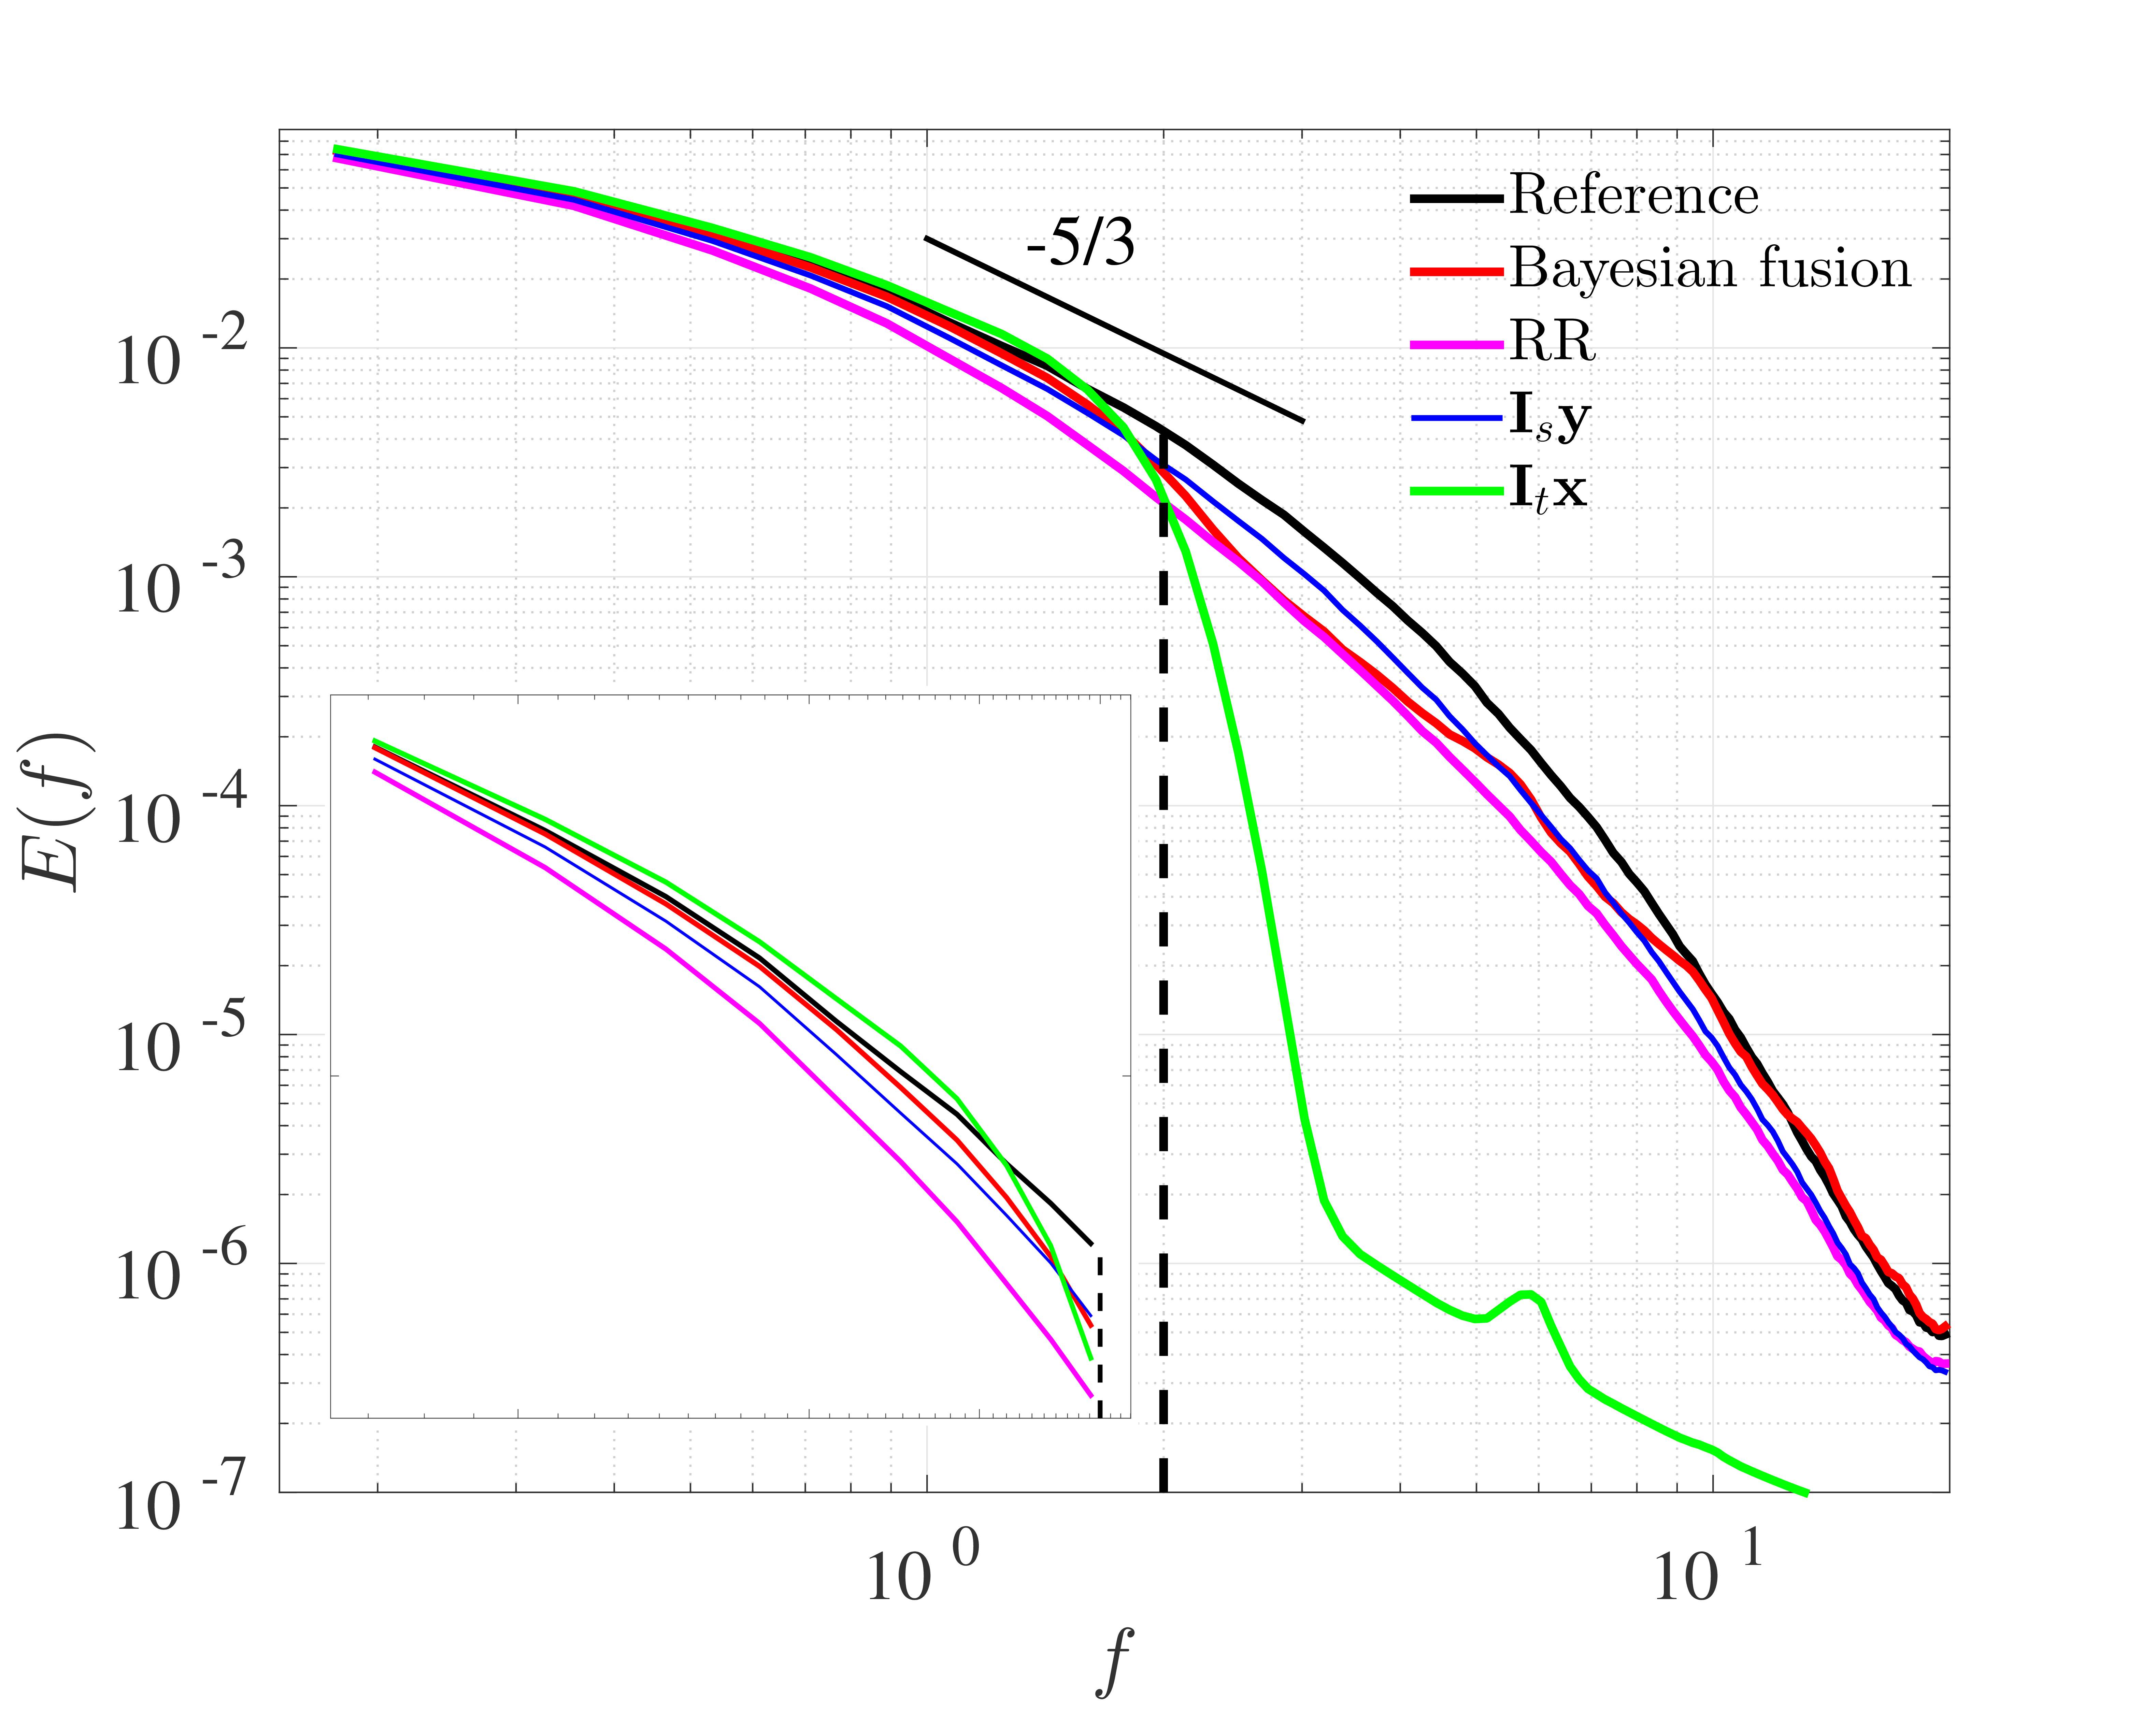
\includegraphics[width=0.8\columnwidth]{./images/comparisons/channel/improper_sspacing_10_tspacing_10_spectrum_time_joint.png}
\caption{\label{fig:final_channel_spectra} Channel flow: spectra of the fluctuating velocity in figure \ref{fig:final_channel_timeseries}.}
\end{center}
\end{figure}

Temporal spectra, estimated from the same points as those shown in figure \ref{fig:final_channel_timeseries}, are compared in figure \ref{fig:final_channel_spectra}. Time interpolation fails to estimate the signal at higher frequencies than a certain cutoff. RR reconstructs both large and small scales, but the loss of large scale energy is critical. This loss is highlighted in the zoom-in picture of low frequencies. The present model improves the estimation at both low and high frequencies.

\begin{figure}
\begin{center}
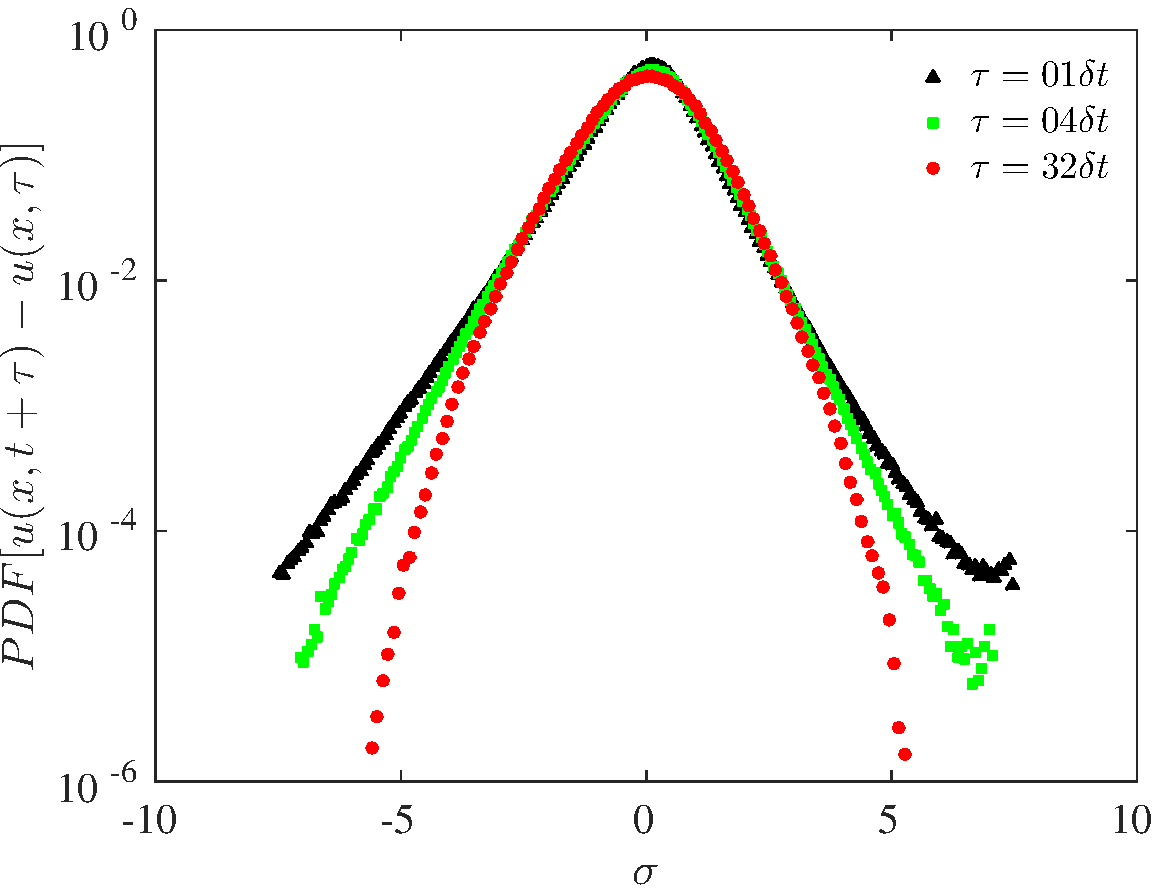
\includegraphics[width=0.49\columnwidth]{./images/comparisons/channel/pdf_org}
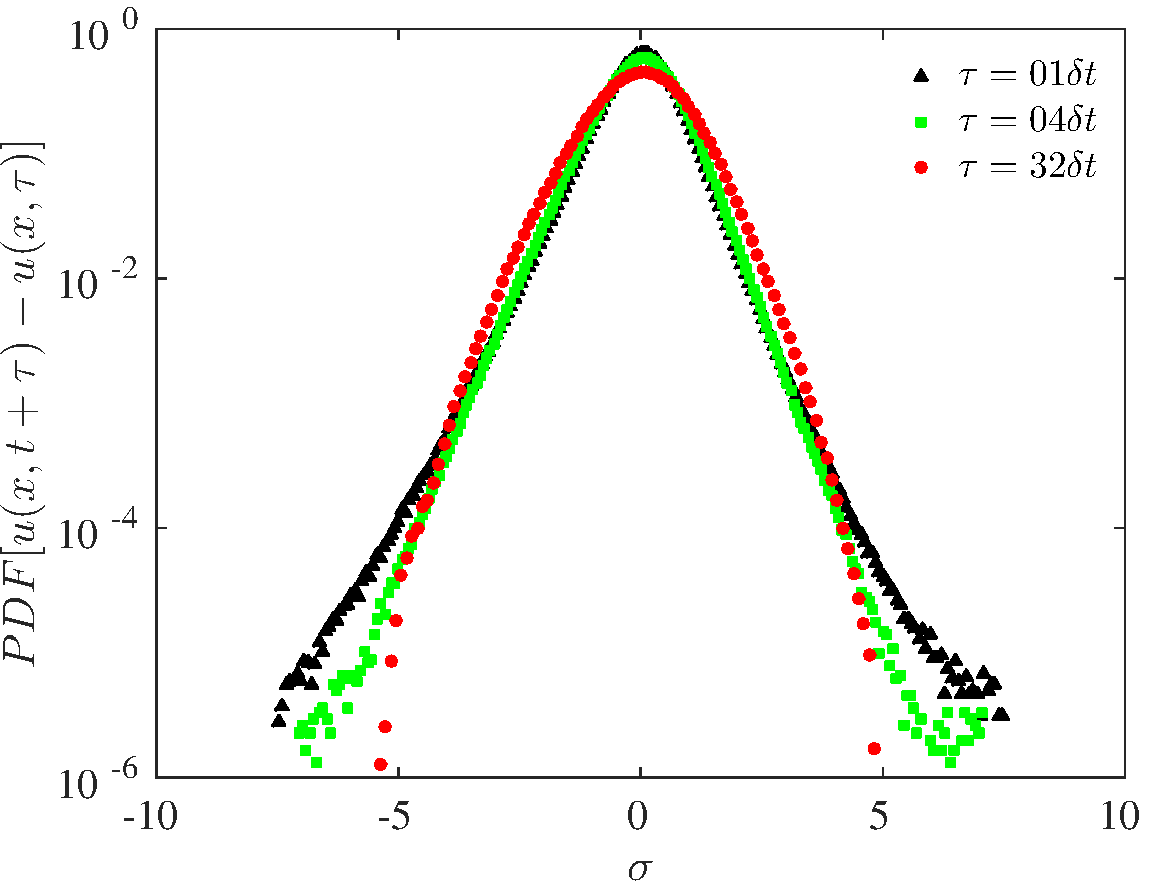
\includegraphics[width=0.49\columnwidth]{./images/comparisons/channel/pdf_fusion}
\caption{\label{fig:final_channel_pdf} Channel flow: probability distribution functions of velocity increments in (left) the original DNS and (right) the reconstructed field.}
\end{center}
\end{figure}

Figure \ref{fig:final_channel_pdf} shows estimates of the probability density functions of time increments $u(x,t+\tau)-u(x,t)$ for the original DNS field as well as for the reconstructed field. As expected, the original field displays intermittent non Gaussian distributions. More importantly, the reconstructed field, while less intermittent, still clearly exhibits non Gaussian increments at small scales. Note that the reconstruction error is essentially due to the difficulty to accurately reconstruct these small scales. It is expected that any reconstruction method will lead to fields that are less intermittent than the original one.

\begin{figure}
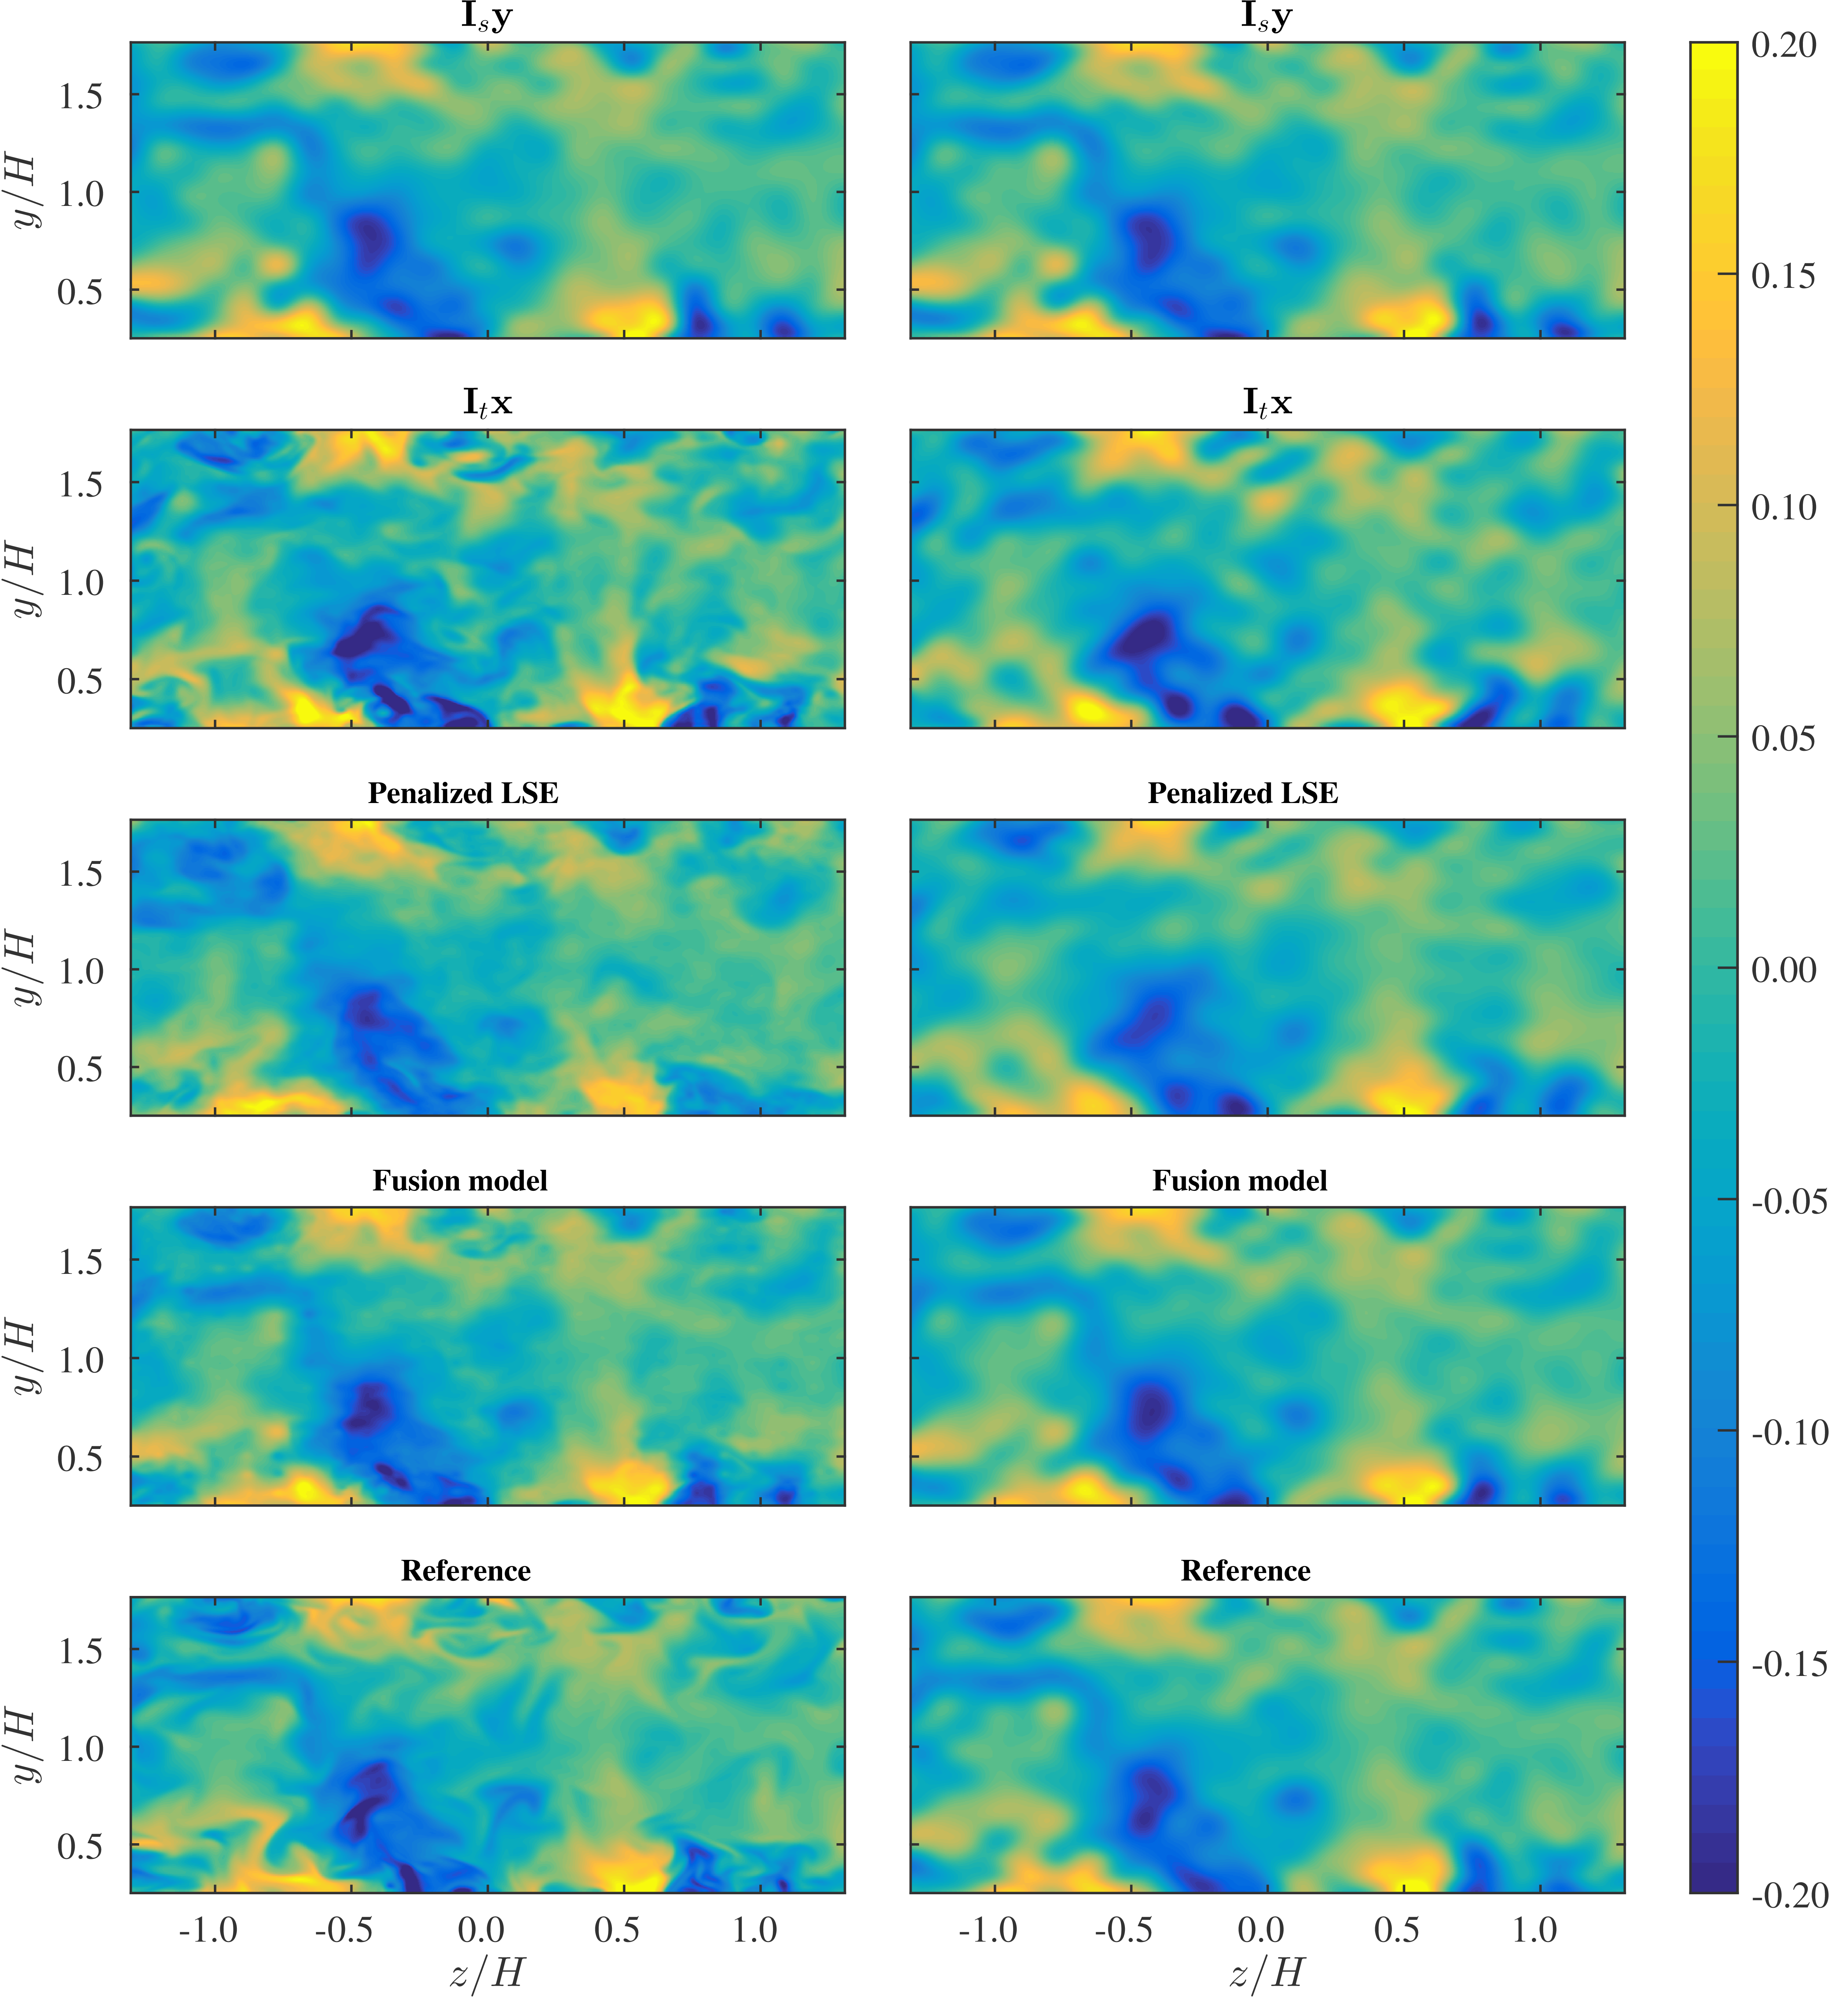
\includegraphics[width=\textwidth]{./images/comparisons/channel/improper_outer_spacespacing_10_timespacing_10_subplots_all_t006.png}
\caption{\label{fig:final_channel_fields} Channel flow: a sample snapshot of fluctuating streamwise velocity at one of the most difficult instant to estimate (in the middle of two LTHS time steps): Reconstruction of all scales (left) and large scales only (right). The figure is better viewed on screen.}
\end{figure}

Figure \ref{fig:final_channel_fields} compares reconstructed snapshots by different methods. This snapshot is at the most remote instant from its two neighboring LTHS time steps. The model reconstructs correctly the velocity field with more flow details than spatial interpolation. It also recovers better large scales than RR and time interpolation methods.

\section{Concluding remarks}
This section analyzes performances of all the models discussed in this thesis. All reconstructions are gathered and compared to highlight the behaviors of different models. These comparisons also suggest further ideas to improve the models by combining several of them to take advantage of different sources of information. 

Two datasets have been used, the DNS data of an isotropic turbulence and a turbulent channel flow at a moderate Reynolds number. Only the streamwise velocity component is studied, but all results can be reproduced for other components. In all configurations, HTLS and LTHS measurements are used as complementary information in space and time. Empirical models find the relation between large and small scales, while fusion models combine two sources of measurements. Only the cases of balanced energy losses are investigated, since otherwise fusion models give results similar to single interpolation of the measurements with the lower energy loss.

Performances of regression models depend only on the subsampling ratio in space. This was expected since these models are not designed to take advantage of information in time. The benefits of such models are highlighted only in comparison to spatial interpolation. The improvements are significant. Kernel regression models also show their superiority compared to linear ones. This is certainly due to the non-linear relation between large and small scales in turbulence.

NLM-based propagation models reconstruct the small scales using a different prior. Small scales are assumed to be advected by larger ones. These small-scale information are then propagated along the time direction based on the similarity levels of corresponding large scales in space. Results show some advantages especially when the subsampling ratios are small in both space and time. A ratio of $ 3 \times 3 $ in space, corresponding to about $ 1\% $ of energy loss, ensures that the model does not start from a too severe loss of information. In time, a ratio of $ 4 $, also about $ 1\% $ of energy loss, ensures that the similarity level between large scales remains significant. Significant benefits are observed compared to spatial interpolation, even in rather crude subsampling ratios in space and time. A non-greedy scheme, by gradually propagating small scales from LTHS planes, gives slightly better reconstructions compared to the greedy one. 

The analyses show advantages of further exploiting information in time. The Bayesian fusion model, despite its simplicity, demonstrates clear benefits compared to other methods. By simply proposing compromise estimates between the two interpolations in space and time, it leads to more accurate reconstruction at all positions in space and time. The compromise is achieved in the form of a weighted average, where weights are learned from measurements. These weights encode some information about the physics of the flow. Benefits are significant in cases of balanced energy losses. The 2D fields or 1D signal comparisons also demonstrate that the fusion model seeks a trade-off between retaining good large-scale information from a single interpolation and proposes more details from the other interpolation.

All models reconstruct the fields using different priors, i.e. exploiting information differently. Comparisons show clear advantages of combining different measurements. Further exploitations and combinations of such models can improve the reconstruction results. For instance, NLM-based propagation could start from initial large scales obtained from regression, which are more accurate than spatial interpolation. This propagated information, which exploits the local similarity of the flows, could combine with the time interpolation to further improve results of Bayesian fusion models. 


\chapter*{Conclusions and perspectives} 
\label{chap_conclusion_perspectives} 
This work lies in between the two research domains of turbulence and image processing. The main objective was to explore a large spectrum of approaches to estimate small-scale turbulence from given measurements at large scales only. One contribution of the thesis is to review conventional methods. We have also adapted other models inspired from recent works in image processing and proposed new methods to our context. 

The estimation of small-scale turbulence from measurements has been addressed via two problems described in chapter \ref{chap_problem_definition}. The first problem is to find a relationship between large and small scales of turbulence given training samples at all scales. The second is to measure and combine complementary information, which are from space and time in this case. DNS data of an isotropic turbulence and a channel flow are used to setup different numerical experiments. These data give access to all scales of turbulence, which are used as the reference to qualify different approaches. Low-resolution fields of large scales are virtually extracted from the reference ones to which the reconstructions are compared. 

For the two problems, we have proposed two families of approaches. The first one is to learn an empirical relationship between large and small scales through simple regression models or through learning coupled representations of different scales using dictionary learning. The second group of methods is based on the fusion of information. Different assumptions are exploited to propose schemes to combine available measured data. Two fusion models are developed, which use either similarity of structures in the flows or probabilistic models to find compromise estimates given the measurements. 

Chapter \ref{chap_linearregression} reviewed regression models, which find mapping functions between low-resolution and high-resolution fields. The function can be linear (via a set of coefficients) or nonlinear (using fixed kernel spaces). Model performances are usually sensitive to some hyper-parameters. This problem was addressed by optimizing a bias-variance trade-off using the cross-validation technique. Comparing reconstruction results, these models work better than standard spline interpolation. Nonlinear regressions also give more accurate reconstruction than linear ones. 

Chapter \ref{chap_dictionarylearning} discussed \textit{dictionary learning}, a generalization of principal component analysis (called \textit{proper orthogonal decomposition} in turbulence studies) to learn redundant bases that better represent turbulent fields in a sparse manner. A couple of representations are learned and used to reconstruct the high-resolution fields from low-resolution measurements. In the case of direct subsampling that could happen in real experiments, the aliasing problem appears. We observe that the coupled dictionary learning method does not permit to de-alias. The model has not brought significant improvements compared to spatial interpolation. Once avoiding this problem by a prefiltering step, dictionary learning gives significant improvements compared to interpolation. In the range of scale between 0.5 and 1.5 the cutoff, it reduces the energy loss by about $ 60 \% $ and the total error by about $ 15 \% $. 

Chapter \ref{chap_NLM} discussed a non-local means-based propagation model as the first fusion model. The model was based on the hypothesis of \textit{rapid distortion}, which assumes that small scales are advected by large ones. These small-scale information from the LTHS planes are propagated in time based on the similarity level of large scales in space. The model works very well at low subsampling ratios in space and time (corresponding to about $ 1\% $ of energy loss) where it significantly improves the reconstruction accuracy (by about $ 40\% $) compared to single interpolation in space. However, the model is not very robust when the energy losses are more severe. With large subsampling ratios in space (for instance $ \dimsh/\dimsl =6 \times 6 $), it suffers from severe losses and can not recover completely even at large-scale. With large ratios in time (for instance $ \dimth/\dimtl = 8 $) , similarities of large scales decay rapidly and make propagation models less accurate.

To further exploit all available information from measurements, a simple yet efficient fusion model was proposed in chapter \ref{chap_BayesianFusion}. The model estimates a high-resolution field that maximizes its \textit{posterior} probability given the measurements. A Bayesian framework is used and further simplifications lead to a linear fusion formula, a weighted sum of the two single interpolations from the two measured data. Weighted coefficients are covariance matrices of unknown small scales, which are learned from measurements. The model reconstructs high-resolution fields with significant improvement compared to single interpolations from either sources. The superiority of this model is emphasized in the case where energy losses are balanced in space and time. In such cases, improvements are observed both at large and small scales.

Chapter \ref{chap_comparisons} provided a more global view of all proposed methods. We synthesized reconstructions by all approaches for the same setups where measurements in space and time are subsampled in a balanced manner. Dictionary learning is omitted in this comparison because of its slightly different configuration of numerical experiments. Single models to solve the reconstruction problem can be predefined (interpolation) or learned adaptively from the training data (regression). Adaptive models reconstruct the fields more accurately. More significant improvements are observed when combining complementary measurements in space and time. NLM-based model gives very accurate reconstructions at low energy losses. At higher subsampling ratios, this model is not able to over-perform temporal interpolation. Bayesian fusion model is simpler yet more efficient, and gives the best reconstruction in all cases. 

\subsection{Suggestions for future works}
The main purpose of this work was a first exploration of a set of methods for the reconstruction of fully resolved turbulent fields from low resolution measurements. Turbulent fields are highly disordered and much less regular than natural images, therefore the inverse problem of reconstruction is even more difficult in our case. This thesis has opened many new directions to develop tools for turbulence studies. Results have suggested also some new directions for signal/image processing studies to provide even more adapted tools. The present work gives rise to the following suggestions for future works.

\subsubsection*{Extending to the reconstruction of three-component velocity fields?} 
The whole thesis has dealt with the reconstruction of streamwise velocity fields. All results can be reproduced for the other two components independently. However, all components are connected physically through Navier-Stokes equations. Further investigations are needed to exploit the information such as cross-correlation between components, vorticities and divergence of the velocity fields. One idea is to impose the prior of \textit{divergence-free}. Another idea would be to use vorticities as features instead of derivatives to learn coupled dictionaries.  

\subsubsection*{Ensemble of models as generalizing Bayesian fusion model?} 
Chapter \ref{chap_comparisons} has compared performances of all proposed models. It has shown that different models, though exploiting different sources of information or assumptions, give better results than single interpolations. Combining multi-sources of measurements through their interpolations gives more accurate reconstructions compared to one complex single model. This observation suggests to further ensemble different models and take advantage of each single model. Regressions, by learning an adaptive interpolator, could replace spline interpolations. NLM-based propagation models by exploiting the similarity information also appear as a good candidate to replace simple interpolation. 

\subsubsection*{Highly nonlinear mapping function between large and small scales of turbulence?} This thesis has reviewed regression models, but they remain rather simplistic to describe this highly nonlinear relation between scales. This is suggested when observing advantages of kernel regressions in chapter \ref{chap_comparisons}. Other ideas, especially \textit{neural network} and \textit{deep learning} \citep{dong2014image}, could be studied. Such approaches permit much more complex and highly nonlinear mapping functions between input low-resolution and output high-resolution fields, not restricted to a fixed kernel space as the KRR model. However, such a model requires an extremely large amount of training samples. The patch-wise approach is potentially a good candidate to give access to more samples and to localize the information. Such models could be combined with sparse prior \citep{wang2015deep} discussed in chapter \ref{chap_dictionarylearning} and proven to further improve reconstruction accuracy. 

\subsubsection*{Dictionary learning for other inverse problems in turbulence?} As a more efficient representation compared to PCA and predefined wavelets, dictionary learning has demonstrated its possibility to solve the inverse problem of reconstructing high-resolution velocities from low-resolution measurements. The improvement is significant when aliasing is handled carefully but inoperative in the case of direct subsampling. This approach is not limited to super-resolution only. Other inverse problems such as removing noise or estimating missing pixels could be studied. One particular idea is to apply dictionary learning to D time-resolved experimental data of ``\textit{Shake-The-Box}''-PIV \citep{schroder2015advances}. By following the particles, the method resolves till pixel size. However, velocity fields in a uniform grid is estimated by simple interpolations. This could be done with dictionary learning. Viewing the fields with many missing pixels as random sensing, the approach could learn the missing small scales from the position it ``\textit{sees}'' and propose better estimates than interpolation. Also, measurements noise could be separated from the true information in the same step. 

\subsubsection*{Dictionary learning to deal with aliasing from direct subsampling?} Aliasing is a known problem when the sensing system directly subsamples the fields without the prefiltering step. The first attempt of dictionary learning to reconstruct the high-resolution fields from the subsampled measurements has failed potentially due to aliasing. Without its presence, the model gives clear improvements compared to single interpolation. The problem of removing aliasing could be addressed and solved using dictionary learning as well. Coupled dictionaries could be learned to represent the fields with and without aliasing. The model in chapter \ref{chap_dictionarylearning} would become a three-stage super-resolution model, with an intermediate step to remove aliasing.

\subsubsection*{A more complete fusion model, a Bayesian way?} The fusion model proposed in this work uses only a very simple weighted sum formula. The prior of the estimated field is omitted from the formula due to the assumption of a non-informative prior. Full covariance matrices to represent all sources of space-time correlations are also simplified to diagonal ones. Some work remains to be done to further exploit the information from measurements by building more complete covariance matrices. Also, a good prior could further improve further the reconstruction. The prior could carry physical properties of the flow, for example divergence free, energy spectra or even full Navier-Stokes equations. In case the full fields are given as training data, covariance matrices could also be learned adaptively. In such cases, the weights of the fusion model could be learned to take the properties of turbulence into account. 

\subsubsection*{Combining fusion and dictionary learning?} Dictionary learning has shown to be a good representation of turbulent fields using a sparsity prior. This prior helps in solving the ill-posed problem of reconstructing high-resolution fields. Fusion models by combining multi-sources of measurements are simple but also very efficient to solve the problem. The idea of combining sparse prior and fusion could be studied, inspired by \citet{wei2015hyperspectral}. In chapter \ref{chap_BayesianFusion}, the optimization problem is:
\begin{equation}
	\z = \argmin_{\z} \left\lbrace \frac{1}{2} \Mdist{\z -\Interp_t\x}{\Sigma_{\h_t}} + \frac{1}{2}\Mdist{\z -\Interp_s\y}{\Sigma_{\h_s}} \right\rbrace
\end{equation}
By imposing the sparse prior, the problem could be rewriten as:
\begin{equation}
	\z = \dict \dictco \subjectto \{\dict,\dictco\} = \argmin_{\dict,\dictco} \left\lbrace \frac{1}{2} \Mdist{\dict \dictco -\Interp_t\x}{\Sigma_{\h_t}} + \frac{1}{2}\Mdist{\dict\dictco -\Interp_s\y}{\Sigma_{\h_s}} + \lambda \normone{\dictco} \right\rbrace
\end{equation}
or avoiding the interpolations, hence not bringing aliasing terms into the system, as:
\begin{equation}
		\z = \dict \dictco \subjectto \{\dict,\dictco\} = \argmin_{\dict,\dictco} \left\lbrace \frac{1}{2} \Mdist{\Sub_t\dict \dictco -\x}{\Sigma_{\h_t}} + \frac{1}{2}\Mdist{\Sub_s\dict\dictco -\y}{\Sigma_{\h_s}} + \lambda \normone{\dictco} \right\rbrace
\end{equation}
Solving the above highly non-convex problem could be addressed thanks to recent progresses in solving alternating optimization problems \citep{boyd2011distributed,parikh2014proximal}. 

\subsubsection*{Increase resolution of PIV measurements using different setups?} Regression and interpolation are restricted to reconstruct high-resolution fields from low-resolution ones at the same scene, while it is not the case for coupled dictionaries learning. One very promising setup would be to combine high-resolution PIV with time-resolved PIV (Tr-PIV). High-resolution PIV can measure the flow at a small field-of-view but at very high spatial resolution. These measurements could be used to train the dictionaries. Then Tr-PIV measures the flow at a much larger field-of-view but at lower resolution. Using the trained dictionaries, one could estimate time-resolved velocity fields at large field-of-view and high spatial resolution. One should notice also the limitation of such an approach in de-aliasing to carefully design the sensing system. Another configuration could be to use two different PIV systems to measure HTLS and LTHS fields (see figure \ref{fig:space-time_measurements}) and apply fusion models to maximize the level of useful information.

\subsubsection*{Co-conception design of experiments?} The thesis has studied the performances of various models for different configurations at various subsampling ratios. This gives an idea of which method to choose for one particular setup. From a certain loss of energy due to subsamplings, this work suggests the maximum level of accuracy and scale one could expect to reconstruct. This information is very useful to design new challenging experiments in order to maximize the expected level of small scale content after post-processing. This thesis connects to the current research area of co-conception. The idea is to co-design the measurement system with respect to some pre-defined post-processing procedure. 

\printbibliography

%%%%%%%%%%%%%%%%%%%%%%%%%%%%%%%%%%%%%%%%%%%%%%%%%%%%%%%%%%%%%%%%%%%%%%%%%%%%%%%
% Début de la partie annexe éventuelle
%%%%%%%%%%%%%%%%%%%%%%%%%%%%%%%%%%%%%%%%%%%%%%%%%%%%%%%%%%%%%%%%%%%%%%%%%%%%%%%
\appendix
\chapter{Bayesian framework}
\label{apx_BayesGausvars}

\section{Derivation of Linear Gaussian models}
\label{apx_BayesGausvars_1}
\subsection{Bayes' theorem for Gaussian variables}
Let $ \mybold{v} $ is the measurement, then the probability $ p(\mybold{v}) $ is known. Let $ \mybold{u} $ is the desired variable, with the prior distribution $ p(\mybold{u}) $. Suppose also there exists a linear observation model:
\begin{equation}
	\mybold{v}=A\mybold{u}+\mybold{n}
\label{eq:LG5}
\end{equation}
where $ \mybold{n} $ is a zero-mean random vectors and independent on $ \mybold{u} $ and $ \mybold{v} $ and has a precision matrix denoted as $ \Lambda_{\mybold{v}|\mybold{u}}= \Sigma_{\mybold{v}|\mybold{u}}^{-1}$. One can express the joint probability $ p(\mybold{w})$ as the product of the prior probability $ p(\mybold{u}) $ and the likelihood function of the measurement given the variable $ p(\mybold{v}|\mybold{u})$ as:
\begin{eqnarray}
	p(\mybold{u})=&&\distr(\mybold{u}|\mybold{\mu}_{\mybold{u}},\Lambda^{-1}_{\mybold{u}}) \\
	p(\mybold{v}|\mybold{u})=&&\distr(\mybold{v}|A\mybold{\mu}_{\mybold{u}},\Lambda_{\mybold{v}|\mybold{u}}^{-1})
\label{eq:LG6}
\end{eqnarray}
To derive, let take the natural logarithm of both sides, using also the symmetrical shape of precision matrices,  the left hand side gives:
\begin{eqnarray}
	ln \: p(\mybold{w}) =&& -\frac{1}{2} \left(\mybold{w}-\mybold{\mu}_{\mybold{w}} \right)^T \Lambda_{\mybold{w}} \left(\mybold{w}-\mybold{\mu}_{\mybold{w}} \right) + const \nonumber\\
	=&& -\frac{1}{2} \mybold{w}^T \Lambda_{\mybold{w}} \mybold{w} +\mybold{w}^T \Lambda_{\mybold{w}} \mybold{\mu}_{\mybold{w}} \nonumber\\
	&& - \frac{1}{2} \mybold{\mu}_{\mybold{w}} \Lambda_{\mybold{w}} \mybold{\mu}_{\mybold{w}} + const
	\label{eq:LG7}
\end{eqnarray}
and the right hand side gives:
\begin{eqnarray}
	ln \left(p(\mybold{u}) p(\mybold{v}|\mybold{u}) \right) =&& \left(\mybold{u}-\mybold{\mu}_{\mybold{u}} \right)^T \Lambda_{\mybold{u}} \left(\mybold{u}-\mybold{\mu}_{\mybold{u}} \right) \nonumber\\
	&&- \frac{1}{2} \left( \mybold{v}-A\mybold{u} \right)^T \Lambda_{\mybold{v}|\mybold{u}} \left( \mybold{v}-A\mybold{u} \right) \nonumber\\
	&&+ const
\label{eq:LG8}
\end{eqnarray}
In above equations, $ const $ represents all the terms that are independent on $ \mybold{u} $ and $\mybold{v}$. The first order terms in the above equation include:
\begin{eqnarray}
	1^{st} \: order \: terms =&& \mybold{u}^T  \Lambda_{\mybold{u}} \mybold{\mu}_{\mybold{u}} - \mybold{u}^T A^T\Lambda_{\mybold{v}|\mybold{u}} \nonumber\\
	=&&  \left(\begin{matrix}\mybold{u}\\\mybold{v} \end{matrix}\right)^T  \left(\begin{matrix}\Lambda_{\mybold{u}}{\mu}_{\mybold{u}} \\ 0 \end{matrix}\right)
\label{eq:LG9}
\end{eqnarray}
and the second order terms are:
\begin{eqnarray}
	2^{nd} \: order \: terms = && -\frac{1}{2} \mybold{u}^T \left( \Lambda_{\mybold{u}}+A^T \Lambda_{\mybold{v}|\mybold{u}} A \right)\mybold{u}  - \frac{1}{2} \mybold{v}^T \Lambda_{\mybold{v}|\mybold{u}} \mybold{v} \nonumber\\
	&& + \frac{1}{2} \mybold{v}^T \Lambda_{\mybold{v}|\mybold{u}} A \mybold{u} + \mybold{u}^T A^T \Lambda_{\mybold{v}|\mybold{u}} \mybold{v} \nonumber\\
	=&& -\frac{1}{2} \left(\begin{matrix}\mybold{u}\\\mybold{v} \end{matrix}\right)^T  \left(\begin{matrix}A^T\Lambda_{\mybold{v}|\mybold{u}}A+\Lambda_{\mybold{u}} & A^T\Lambda_{\mybold{v}|\mybold{u}} \nonumber\\ -\Lambda_{\mybold{v}|\mybold{u}} A & \Lambda_{\mybold{v}|\mybold{u}}\end{matrix}\right) \left(\begin{matrix}\mybold{u}\\\mybold{v} \end{matrix}\right) \\
	=&& -\frac{1}{2} \mybold{w}^T \Lambda_{\mybold{w}} \mybold{w}
\label{eq:LG10}
\end{eqnarray}
Comparing above equations \ref{eq:LG10}, \ref{eq:LG9} and \ref{eq:LG7}, Gaussian distribution of $ \mybold{w} $ takes the precision matrix $ \Lambda_{\mybold{w}} $ of the form:
\begin{equation}
	\Lambda_{\mybold{w}}= \left(\begin{matrix}\Lambda_{\mybold{u}\mybold{u}} & \Lambda_{\mybold{u}\mybold{v}} \\ \Lambda_{\mybold{v}\mybold{u}} & \Lambda_{\mybold{v}\mybold{v}}\end{matrix}\right) = \left(\begin{matrix}A^T\Lambda_{\mybold{v}|\mybold{u}}A+\Lambda_{\mybold{u}} & A^T\Lambda_{\mybold{v}|\mybold{u}} \\ -\Lambda_{\mybold{v}|\mybold{u}} A & \Lambda_{\mybold{v}|\mybold{u}}\end{matrix}\right)
\label{eq:LG11}
\end{equation}
and the mean $ \mybold{\mu}_{\mybold{w}} $ is:
\begin{equation}
	\mybold{\mu}_{\mybold{w}} = \left(\begin{matrix}\mybold{\mu}_{\mybold{u}} \\ \mybold{\mu}_{\mybold{v}} \end{matrix}\right) = \Lambda_{\mybold{w}}^{-1}\left(\begin{matrix}\Lambda_{\mybold{u}}\mybold{\mu}_{\mybold{u}} \\ 0 \end{matrix}\right) =\Sigma_{\mybold{w}} \left(\begin{matrix}\Lambda_{\mybold{u}}\mybold{\mu}_{\mybold{u}} \\ 0 \end{matrix}\right)
\label{eq:LG12}
\end{equation}
The covariance matrix is obtained by taking the inverse of above:
\begin{equation}
	\Sigma_{\mybold{w}}=\left(\begin{matrix}\Sigma_{\mybold{u}\mybold{u}} & \Sigma_{\mybold{u}\mybold{v}} \\ \Sigma_{\mybold{v}\mybold{u}} & \Sigma_{\mybold{v}\mybold{v}}\end{matrix}\right) = \left(\begin{matrix}A^T\Lambda_{\mybold{v}|\mybold{u}}A+\Lambda_{\mybold{u}} & A^T\Lambda_{\mybold{v}|\mybold{u}} \\ -\Lambda_{\mybold{v}|\mybold{u}} A & \Lambda_{\mybold{v}|\mybold{u}}\end{matrix}\right)^{-1} 
\label{eq:LG13}
\end{equation}
Using the inversion lemma:
\begin{equation}
	\left(\begin{matrix} A & B \\ C & D \end{matrix}\right)^{-1}= \left(\begin{matrix}M & -MBD^{-1} \\ D^{-1}+D^{-1}CM & D^{-1}CMBD^{-1}\end{matrix}\right)
\label{eq:LG14}
\end{equation}
where $ M=(A-BD^{-1}C)^{-1} $ is the \textit{Schur complement} of the matrix inversion with respect to $ D $. The covariance matrix is finally given as:
\begin{equation}
	\Sigma_{\mybold{w}}= \left(\begin{matrix}\Sigma_{\mybold{u}\mybold{u}} & \Sigma_{\mybold{u}\mybold{v}} \\ \Sigma_{\mybold{v}\mybold{u}} & \Sigma_{\mybold{v}\mybold{v}}\end{matrix}\right) =\left(\begin{matrix}\Lambda^{-1}_{\mybold{u}} & \Lambda^{-1}_{\mybold{u}}A^T \\ A \Lambda^{-1}_{\mybold{u}} &\Lambda^{-1}_{\mybold{v}|\mybold{u}} + A\Lambda^{-1}_{\mybold{u}}A^T\end{matrix}\right)
\label{eq:LG15}
\end{equation}
Replacing this covariance matrix to equation (\ref{eq:LG13}), the expectation of $ \mybold{w} $ is given as:
\begin{equation}
	\mybold{\mu}_{\mybold{w}} = \left(\begin{matrix}\mybold{\mu}_{\mybold{u}} \\ \mybold{\mu}_{\mybold{v}} \end{matrix}\right) =\left(\begin{matrix}\Lambda^{-1}_{\mybold{u}} & \Lambda^{-1}_{\mybold{u}}A^T \\ A \Lambda^{-1}_{\mybold{u}} & \Lambda^{-1}_{\mybold{v}|\mybold{u}} + A\Lambda^{-1}_{\mybold{u}}A^T\end{matrix}\right) \left(\begin{matrix}\Lambda_{\mybold{u}}\mybold{\mu}_{\mybold{u}} \\ 0 \end{matrix}\right) = \left(\begin{matrix}\mybold{\mu}_{\mybold{u}} \\ A\mybold{\mu}_{\mybold{u}} \end{matrix}\right)
\label{eq:LG16} 
\end{equation}
From equation \ref{eq:LG15} and \ref{eq:LG16}, the Gaussian distribution of $ \mybold{v} = \distr(\mybold{v}| \mybold{\mu}_{\mybold{v}},\Sigma_{\mybold{v}}) $ is:
\begin{eqnarray}
	\mybold{\mu}_{\mybold{v}} =&& A\mybold{\mu}_{\mybold{u}} \nonumber\\
	\Sigma_{\mybold{v}} =&& \Lambda^{-1}_{\mybold{v}|\mybold{u}} + A\Lambda^{-1}_{\mybold{u}}A^T
\label{eq:LG17}
\end{eqnarray}
Using results of conditional Gaussian distribution as in equation \ref{eq:LG4}, the posterior ditribution $ \mybold{u}|\mybold{v} $ is $ \distr \left(\mybold{u}|\mybold{\mu}_{\mybold{u}|\mybold{v}}, \Sigma_{\mybold{u}|\mybold{v}} \right) $ where:
\begin{eqnarray}
	\mybold{\mu}_{\mybold{u}|\mybold{v}} =&& \mybold{\mu}_{\mybold{u}}-\Lambda^{-1}_{\mybold{u}\mybold{u}} \Lambda_{\mybold{u}\mybold{v}} (\mybold{u}-\mybold{\mu}_{\mybold{u}}) \nonumber\\
	\Sigma_{\mybold{u}|\mybold{v}} =&& \Lambda^{-1}_{\mybold{u}\mybold{u}}
\label{eq:LG18}
\end{eqnarray}
Taking the partial precision matrices from equation \ref{eq:LG11}, covariance matrix $ \Sigma_{\mybold{u}|\mybold{v}} $ is given as:
\begin{equation}
	\Sigma_{\mybold{u}|\mybold{v}}= \left(A^T\Lambda_{\mybold{v}|\mybold{u}}A+\Lambda_{\mybold{u}}\right)^{-1} 
\label{eq:LG19}	
\end{equation}
and conditional mean $ \mybold{\mu}_{\mybold{u}|\mybold{v}} $ is as:
\begin{eqnarray}
	\mybold{\mu}_{\mybold{u}|\mybold{v}} =&& \mybold{\mu}_{\mybold{u}}- \left(	A^T\Lambda_{\mybold{v}|\mybold{u}}A+\Lambda_{\mybold{u}} \right) ^{-1} \left( -A^T\Lambda_{\mybold{v}|\mybold{u}} \right) \left( \mybold{v}- A\mybold{\mu}_{\mybold{u}} \right) \nonumber\\
	=&& \left(	A^T\Lambda_{\mybold{v}|\mybold{u}}A+\Lambda_{\mybold{u}} \right)^{-1} \left(	A^T\Lambda_{\mybold{v}|\mybold{u}} \mybold{v} +\Lambda_{\mybold{u}}\mybold{\mu}_{\mybold{u}} \right)
\label{eq:LG20}
\end{eqnarray}
Final results written in covariance matrices notation, given:
\begin{eqnarray}
	\mybold{v} =&& A\mybold{u} \nonumber\\
	p(\mybold{u}) =&& \distr \left( \mybold{u}| \mybold{\mu}_{\mybold{u}},\Sigma_{\mybold{u}} \right) \nonumber\\
	p(\mybold{v}|\mybold{u}) =&& \distr \left( \mybold{v}| A\mybold{u},\Sigma_{\mybold{v}|\mybold{u}} \right)
\label{eq:LG21}	
\end{eqnarray}
one gets:
\begin{eqnarray}
	p(\mybold{v}) =&& \distr \left( \mybold{v}| A\mybold{\mu}_{\mybold{u}},\Sigma_{\mybold{v}|\mybold{u}} +A\Sigma_{\mybold{u}}  A^T \right) \nonumber\\
	p(\mybold{u}|\mybold{v}) =&& \distr \left( \mybold{u}| \Sigma_{\mybold{u}|\mybold{v}} \left(	A^T\Lambda_{\mybold{v}|\mybold{u}} \mybold{v} +\Lambda_{\mybold{u}}\mybold{\mu}_{\mybold{u}} \right),\Sigma_{\mybold{u}|\mybold{v}} \right) \nonumber\\
	\Sigma_{\mybold{u}|\mybold{v}} =&& \left(A^T\Sigma_{\mybold{v}|\mybold{u}}^{-1}A+\Sigma_{\mybold{u}}^{-1}\right)^{-1}
\label{eq:LG22}	
\end{eqnarray}

\subsection{ The model}
As one of the example linear Gaussian model in \cite{roweis1999unifying} and restated in \cite{bishop2006pattern}, given the Gaussian distribution of measurements $p(\mybold{u}) $ and posterior distribution $ p(\mybold{u}|\mybold{v}) $:
\begin{eqnarray}
	p(\mybold{u}) =&& \distr \left( \mybold{u}| \mybold{\mu}_{\mybold{u}},\Sigma_{\mybold{u}} \right) \nonumber\\
	p(\mybold{v}|\mybold{u}) =&& \distr \left( \mybold{v}| A\mybold{u}+\mybold{b},\Sigma_{\mybold{v}|\mybold{u}} \right)
\label{eq:bishop_linear_gaussian_1}	
\end{eqnarray}
where $ \mu_{\mybold{u}} $, $ A $ and $ b $ are parameters governing the mean of the distributions; $ \Sigma_{\mybold{v}|\mybold{u}} $ is not a function of $ \mybold{u} $. Applying Bayes's theorem for these Gaussian variables, the joint distribution can be written using the prior and likelihood distributions given as:
\begin{eqnarray}
	p(\mybold{v}) =&& \distr \left( \mybold{v}| A\mybold{\mu}_{\mybold{u}} + \mybold{b},\Sigma_{\mybold{v}|\mybold{u}} +A\Sigma_{\mybold{u}}  A^T \right) \nonumber\\
	p(\mybold{u}|\mybold{v}) =&& \distr \left( \mybold{u}| \Sigma_{\mybold{u}|\mybold{v}} \left(	A^T\Lambda_{\mybold{v}|\mybold{u}} \left( \mybold{v} - \mybold{b} \right) +\Lambda_{\mybold{u}}\mybold{\mu}_{\mybold{u}} \right),\Sigma_{\mybold{u}|\mybold{v}} \right) \nonumber\\
	\Sigma_{\mybold{u}|\mybold{v}} =&& \left(A^T\Sigma_{\mybold{v}|\mybold{u}}^{-1}A+\Sigma_{\mybold{u}}^{-1}\right)^{-1}
\label{eq:bishop_linear_gaussian_2}	
\end{eqnarray}

Using results in equation \ref{eq:bishop_linear_gaussian_2}, given the posterior distributions $ \distr(\mybold{z}|\varmathbb{I}_t\mybold{x},\Sigma_{\mybold{h}_t}) $ and $ \distr(\mybold{z}|\varmathbb{I}_s\mybold{y},\Sigma_{\mybold{h}_s}) $ in equations \ref{eq:Bayes21} and \ref{eq:Bayes22}, and known distributions of measurements $ \distr \left( \varmathbb{I}_t\mybold{x} |0, \Sigma_{\varmathbb{I}_t\mybold{x}} \right)$ and $ \distr \left( \varmathbb{I}_s\mybold{y} |0, \Sigma_{\varmathbb{I}_s\mybold{y}} \right)$. Results of above section show that one can get the likelihood functions and the prior distribution as:
\begin{eqnarray}
		\varmathbb{I}_t \mybold{x}|\mybold{z} :&& \distr \left(\varmathbb{I}_t \mybold{x}|\Sigma_t \Sigma_{\mybold{h}_t}^{-1} \mybold{z},\Sigma_t \right) \nonumber\\
		\varmathbb{I}_s \mybold{y}|\mybold{z} :&& \distr \left(\varmathbb{I}_s \mybold{y}|\Sigma_s \Sigma_{\mybold{h}_s}^{-1} \mybold{z},\Sigma_s \right) \nonumber\\
		\mybold{z} :&& \distr \left(\mybold{z}|0, \Sigma_{\mybold{z}}\right) 
\label{eq:bishop_linear_gaussian_3}	
\end{eqnarray}
where:
\begin{eqnarray}
		\Sigma_t^{-1} =&& \Sigma_{\mybold{h}_t}^{-1} + \Sigma_{\varmathbb{I}_t\mybold{x}}^{-1} \nonumber\\
		\Sigma_s^{-1} =&& \Sigma_{\mybold{h}_s}^{-1} + \Sigma_{\varmathbb{I}_s\mybold{y}}^{-1} \nonumber\\
		\Sigma_{\mybold{z}} =&& \Sigma_{\mybold{h}_t}+\Sigma_{\varmathbb{I}_t\mybold{x}} = \Sigma_{\mybold{h}_s}+\Sigma_{\varmathbb{I}_s\mybold{y}}
\label{eq:bishop_linear_gaussian_4}	
\end{eqnarray}
Using above resulting Gaussian distributions, The MAP estimation of $ \mybold{z} $ is given as:
\begin{eqnarray}
	\hat{\mybold{z}} =&& \underset{\mybold{z}}{argmax} \left\lbrace  p(\varmathbb{I}_t\mybold{x}|\mybold{z})p(\varmathbb{I}_s\mybold{y}|\mybold{z})p(\mybold{z}) \right\rbrace \nonumber\\
	=&& \underset{\mybold{z}}{argmin} \left\lbrace -\ln p(\varmathbb{I}_t\mybold{x}|\mybold{z}) -\ln p(\varmathbb{I}_s\mybold{y}|\mybold{z}) -\ln p(\mybold{z}) \right\rbrace
\label{eq:bishop_linear_gaussian_5}
\end{eqnarray}
Logarithm of above probabilities are given as:
\begin{eqnarray*}
	-2\ln p(\varmathbb{I}_t\mybold{x}|\mybold{z}) =&& \left(\varmathbb{I}_t\mybold{x}-\Sigma_t \Sigma_{\mybold{h}_t}^{-1}\mybold{z} \right)^T \Sigma^{-1}_t \left(\varmathbb{I}_t\mybold{x}-\Sigma_t \Sigma_{\mybold{h}_t}^{-1}\mybold{z}\right) \\
	=&& \Arrowvert \Sigma_t \Sigma_{\mybold{h}_t}^{-1}\mybold{z}-\varmathbb{I}_t\mybold{x} \Arrowvert^2_{\Sigma_t}\\
	-2\ln p(\varmathbb{I}_s\mybold{y}|\mybold{z}) =&&  \left(\varmathbb{I}_s\mybold{y}-\Sigma_s \Sigma_{\mybold{h}_s}^{-1}\mybold{z} \right)^T \Sigma^{-1}_s \left(\varmathbb{I}_s\mybold{y}-\Sigma_s \Sigma_{\mybold{h}_s}^{-1}\mybold{z}\right)\\
	=&& \Arrowvert \Sigma_s \Sigma_{\mybold{h}_s}^{-1}\mybold{z}-\varmathbb{I}_s\mybold{y} \Arrowvert^2_{\Sigma_s}\\
	-2\ln p(\mybold{z}) =&& \mybold{z}^T \Sigma^{-1}_z \mybold{z} = \Arrowvert \mybold{z} \Arrowvert^2_{\Sigma_{\mybold{z}}}
\label{eq:bishop_linear_gaussian_6}
\end{eqnarray*}
The cost function $ C(\mybold{z}) $ is defined as the sum of above terms:
\begin{equation}
	C(\mybold{z}) =\Arrowvert \Sigma_t \Sigma_{\mybold{h}_t}^{-1}\mybold{z}-\varmathbb{I}_t\mybold{x} \Arrowvert^2_{\Sigma_t}  + \Arrowvert \Sigma_s \Sigma_{\mybold{h}_s}^{-1}\mybold{z}-\varmathbb{I}_s\mybold{y} \Arrowvert^2_{\Sigma_s} \Arrowvert \mybold{z} \Arrowvert^2_{\Sigma_{\mybold{z}}}
\label{eq:bishop_linear_gaussian_7}
\end{equation}
 The gradient of $ C(\mybold{z}) $ is computed as:
\begin{eqnarray}
	\frac{\partial C(\mybold{z})}{2\partial \mybold{z}} =&& \Sigma^{-1}_t \left( \Sigma_t \Sigma_{\mybold{h}_t}^{-1}\mybold{z}-\varmathbb{I}_t\mybold{x} \right) + \Sigma^{-1}_s \left( \Sigma_s \Sigma_{\mybold{h}_s}^{-1}\mybold{z}-\varmathbb{I}_s\mybold{y} \right) +\Sigma^{-1}_{\mybold{z}} \mybold{z} \nonumber\\
	=&& \left( \Sigma_{\mybold{h}_t}^{-1} + \Sigma_{\mybold{h}_s}^{-1} + \Sigma^{-1}_{\mybold{z}} \right) \mybold{z} - \left( \Sigma^{-1}_t\varmathbb{I}_t\mybold{x} + \Sigma^{-1}_s\varmathbb{I}_s\mybold{y} \right)
\label{eq:bishop_linear_gaussian_8}	
\end{eqnarray}
The estimation of optimized $ \hat{\mybold{z}} $ is obtained when setting this gradient to zeros:
\begin{equation}
	\hat{\mybold{z}}=\left( \Sigma_{\mybold{h}_t}^{-1} + \Sigma_{\mybold{h}_s}^{-1} + \Sigma^{-1}_{\mybold{z}} \right)^{-1} \left(\Sigma^{-1}_t\varmathbb{I}_t\mybold{x} +\Sigma^{-1}_s\varmathbb{I}_s\mybold{y}\right)
\label{eq:bishop_linear_gaussian_9}
\end{equation}

\section{Derivation of generalized Millman formula}
\label{apx_BayesGausvars_2}
Let denote $ \left\lbrace \hat{\mybold{z}}_1,...,\hat{\mybold{z}}_K \right\rbrace  $ be K estimates of an unknown random vector $ \mybold{z} \in R^n $. The objective of the fusion model is to find the best linear estimate via a set of coefficient matrices $ C_i $ (i=1,...,K):
\begin{equation}
\hat{\mybold{z}}=\sum\limits_{i=1}^{K}{C_i\hat{\mybold{z}}_i} \:\:\:\:\:\:\:\:\: s.t \:\:\:\:\:\:\:\:\: \sum\limits_{i=1}^{K}{C_i}=I_n
\end{equation}
where the weighting matrices are estimated as:
\begin{equation}
\left\lbrace C_i \right\rbrace_{i=1,...,K}=\argmin_{C_i} \left\| \mybold{z}-\sum_{i=1}^{K}{C_i\hat{\mybold{z}}_i} \right\|^2_2 \:\:\:\:\:\:\:\:\: s.t \:\:\:\:\:\:\:\:\: \sum_{i=1}^{K}{C_i}=I_n
\end{equation}
Define the loss function $ J $ as the error expectation:
\begin{equation}
J=E\left\lbrace \left\|  \mybold{z}-\sum\limits_{i=1}^{K}{C_i\hat{\mybold{z}}_i} \right\| ^2_2 \right\rbrace 
\end{equation}
Define also the total error covariance:
\begin{align}
	\Sigma &\triangleq \cov{ \mybold{z}-\hat{\mybold{z}}}  \\ 
	&= \E {\left(   \mybold{z}-\sum\limits_{i=1}^{K}{C_i\hat{\mybold{z}}_i} \right) \left(   \mybold{z}-\sum\limits_{j=1}^{K}{C_j\hat{\mybold{z}}_j} \right)^T}
\end{align}
Since $ \sum_{i=1}^{K}{C_i}=I_n $, the total error covariance is given as:
\begin{equation}
	\Sigma = \E{ \sum\limits_{i=1}^{K}{C_i\left(\mybold{z}-\hat{\mybold{z}}_i \right)}  \sum\limits_{j=1}^{K}{C_j\left(\mybold{z}-\hat{\mybold{z}}_j\right)^T}}
\end{equation}
Define the local error term as $ \tilde{\mybold{z}}_i \triangleq \mybold{z}-\hat{\mybold{z}}_i $ and the local error covariance as $ \Sigma_{ij}\triangleq \cov{\tilde{\mybold{z}}_i,\tilde{\mybold{z}}_j} $, the total error covariance becomes:
\begin{align}
	\Sigma &= \E{\sum\limits_{i,j=1}^{K}{C_i\tilde{\mybold{z}}_i \left(C_j\tilde{\mybold{z}}_j\right)^T}} \\
	&= \sum\limits_{i,j=1}^{K}{C_i\Sigma_{ij}C_j^T}
\end{align}
The loss function $ J $ is rewritten as:
\begin{align}
	J &= E\left\lbrace \left\|  \mybold{z}-\sum\limits_{i=1}^{K}{C_i\hat{\mybold{z}}_i} \right\| ^2_2 \right\rbrace \\
	&= \tr{\sum\limits_{i,j=1}^{K}{C_i\Sigma_{ij}C_j^T}}
\end{align}
Substituting $ C_K=I_n-C_1-C_2-...-C_{K-1} $ into above equation, one gets:
\begin{equation}
\begin{aligned}
J= & \tr{\sum\limits_{i,j=1}^{K-1}{C_i\Sigma_{ij}C_j^T}+\sum\limits_{i,j=1}^{K-1}{\left(C_i\Sigma_{iK}+\Sigma_{Ki}C_i^T\right)}-\sum\limits_{i,j=1}^{K-1}{\left(C_i\Sigma_{iK}C_j^T+C_j\Sigma_{Ki}C_j^T\right)}} \\
& +\tr{\Sigma_{KK}-\left(\sum\limits_{i,j=1}^{K-1}{C_i}\right)\Sigma_{KK}-\Sigma_{KK}\left(\sum\limits_{i,j=1}^{K-1}{C_j^T}\right)+\sum\limits_{i,j=1}^{K-1}{C_i\Sigma_{KK}C_j^T}}
\end{aligned}
\end{equation}
Using the symmetric property of covariance matrices, i.e. $ \Sigma_{ij}=\Sigma_{ji}^T $ and $ \Sigma_{ii}=\Sigma_{ii}^T $, one gets:
\begin{align}
	\frac{\partial}{\partial C_i} \left(\tr{C_i\Sigma} \right) &= \Sigma^T \\
	\frac{\partial}{\partial C_i} \left(\tr{\Sigma C_i^T} \right) &= \Sigma \\
	\frac{\partial}{\partial C_i} \left(\tr{C_i \Sigma C_i^T} \right) &= C_i \left(\Sigma+\Sigma^T \right)
\end{align}
Taking partial derivative $ \partial J / \partial C_i $ and set to zero, one gets:
\begin{equation}
	\sum\limits_{i,j=1}^{K-1}{C_i} \left(\Sigma_{ij}-\Sigma_{iK}\right)+C_K\left(\Sigma_{Kj}-\Sigma_{KK}\right) = 0 \:\:\:\:\: s.t. \:\:\:\:\: \sum\limits_{i,j=1}^{K}{C_i}=I_n, \:\: j=1,...,K-1
\end{equation}
The final GMF of fusing $ \mybold{z} $ from $ \left\lbrace \hat{\mybold{z}}_1,...,\hat{\mybold{z}}_K \right\rbrace  $ is: 
\begin{equation}
\hat{\mybold{z}}=\sum\limits_{i=1}^{K}{C_i\hat{\mybold{z}}_i} \:\:\:\:\: s.t. \:\:\:\:\: \begin{cases}
\sum\limits_{i=1}^{K}{C_i}=I_n\\
\sum\limits_{i,j=1}^{K-1}{C_i} \left(\Sigma_{ij}-\Sigma_{iK}\right)+C_K\left(\Sigma_{Kj}-\Sigma_{KK}\right) = 0, \:\: j=1,...,K-1
\end{cases}
\end{equation} 
with a total error covariance of:
\begin{equation}
\Sigma=\sum\limits_{i,j=1}^{K}{C_i\Sigma_{ij}C_j^T}
\end{equation}

\subsubsection*{Bar-Shalom and Campo (1986)}
In the case of fusing two estimates ($ K=2 $), the GMF becomes Bar-Shalom-Campo formula:
\begin{equation}
\hat{\mybold{z}}=C_1\hat{\mybold{z}}_1+C_2\hat{\mybold{z}}_2
\end{equation}
Weighting matrices $ C_1 $ and $ C_2 $ satisfy:
\begin{equation}
\begin{cases}
C_1+C_2=I_n\\
C_1\left(\Sigma_{11}-\Sigma_{12}\right)+C_2\left(\Sigma_{21}-\Sigma_{22}\right)=0 \\
C_1\left(\Sigma_{12}-\Sigma_{12}\right)+C_2\left(\Sigma_{22}-\Sigma_{22}\right)=0
\end{cases}
\end{equation}
which lead to:
\begin{equation}
\begin{cases}
C_1 = \left(\Sigma_{22}-\Sigma_{21}\right)\left(\Sigma_{11}+\Sigma_{22}-\Sigma_{12}-\Sigma_{21}\right)^{-1}\\
C_2 = \left(\Sigma_{11}-\Sigma_{12}\right)\left(\Sigma_{11}+\Sigma_{22}-\Sigma_{12}-\Sigma_{21}\right)^{-1}
\end{cases}
\end{equation}
In case $ \tilde{\mybold{z}}_1 $ and $ \tilde{\mybold{z}}_2 $ are uncorrelated, i.e. $ \Sigma_{12}=\Sigma_{21}=0 $, the fusion formula is known as the Millman's formula:
\begin{equation}
\hat{\mybold{z}}=\Sigma_{22}\left(\Sigma_{11}+\Sigma_{22}\right)^{-1}\hat{\mybold{z}}_1+\Sigma_{11}\left(\Sigma_{11}+\Sigma_{22}\right)^{-1}\hat{\mybold{z}}_2
\end{equation}
This formula is identical to the Bayesian fusion model assuming a non-informative prior on $ \mybold{z} $.


%%%%%%%%%%%%%%%%%%%%%%%%%%%%%%%%%%%%%%%%%%%%%%%%%%%%%%%%%%%%%%%%%%%%%%%%%%%%%%%
% Début de la partie finale
%%%%%%%%%%%%%%%%%%%%%%%%%%%%%%%%%%%%%%%%%%%%%%%%%%%%%%%%%%%%%%%%%%%%%%%%%%%%%%%
\restoregeometry
\backmatter

% (Facultatif) Index :
\printindex
%
% Table des matières
\tableofcontents
%
% (Facultatif) Production de la 4e de couverture :
\makebackcover
%
\end{document}
